\documentclass[12pt,a4paper]{report}
\usepackage[english]{babel}
\usepackage[T1]{fontenc}
\usepackage{times}
\usepackage{amsmath}
\usepackage{amsfonts}
\usepackage{amssymb}
\usepackage{textcomp}
\usepackage{gensymb}
\usepackage[linkcolor=true]{hyperref}
\usepackage{graphicx}
\usepackage{setspace}
\usepackage[version=4]{mhchem}
\usepackage{caption}
\usepackage{subcaption}
\usepackage{booktabs}
\usepackage{float}
\usepackage{longtable}
\usepackage{multirow}
\usepackage{wrapfig}
\usepackage[left=2cm,right=2cm,top=2cm,bottom=3cm]{geometry}
\usepackage{fancyhdr}
\usepackage{etoolbox}% http://ctan.org/pkg/etoolbox
\usepackage{markdown}
\usepackage[toc,page]{appendix}
\usepackage[table,xcdraw]{xcolor}
\newcommand{\citep}[1]{\cite{#1}}
\newcommand{\vect}[1]{\boldsymbol{#1}}
\makeatletter
\newcommand{\tocfill}{\cleaders\hbox{$\m@th \mkern\@dotsep mu . \mkern\@dotsep mu$}\hfill}
\makeatother
\newcommand{\abbrlabel}[1]{\makebox[3cm][l]{\textbf{#1}\ \tocfill}}
\newenvironment{abbreviations}{\begin{list}{}{\renewcommand{\makelabel}{\abbrlabel}%
                                              \setlength{\itemsep}{0pt}}}{\end{list}}

\makeatletter
\patchcmd{\@makechapterhead}{\vspace*{50\p@}}{}{}{}% Removes space above \chapter head
\patchcmd{\@makeschapterhead}{\vspace*{50\p@}}{}{}{}% Removes space above \chapter* head
\makeatother
\pagestyle{fancy}
\fancyhf{}
\fancyhead[RO]{\textsc{\nouppercase{{\leftmark}}\quad\thepage}}
\fancypagestyle{plain}{%
  \renewcommand{\headrulewidth}{0pt}%
  \fancyhf{}%
}
\setlength{\headheight}{52pt}    

\begin{document}
\begin{titlepage}

\centering

\includegraphics{logo_ulg.jpg}%

\vspace*{1cm}
\hrulefill
\begin{center}\bfseries\Huge
Interpolation of component characteristic maps for thermodynamic cycle assessment
\end{center}
\hrulefill
\vspace*{0.2cm}
\begin{center}\Large
\textit{Master thesis submitted in partial fulfillment of the requirements
for the degree of Master in Electromechanical Engineering}
\end{center}
\begin{center}\Large
\textit{By Heylen Martin}
\end{center}
\vspace*{0.2cm}

\begin{center}\bfseries\large

University of Liege - Faculty of Applied Sciences \\
Academic year: 2019-2020\\
Promotor: Hilleweart Koen
\end{center}
\begin{flushright}

\end{flushright} 

\end{titlepage}

\setstretch{1.5}
\chapter*{Abstract}
\quad\ Since the last decades, there have been many breakthroughs in the development of thermodynamic cycles. This is thanks to the development of the different technologies used during the design and manufacturing phases of the different components (pumps, compressors, turbines, combustion chamber, etc.). By improving their efficiency, it has been possible to increase the compactness of the system. In particular, micro gas turbine based on the Brayton cycle started to be developed. 

The goal of this work is to provide a program written in Python that will assess the performance of different configurations of the Brayton gas cycle. Among the possible configurations, there are the Gas Turbine (GT), Regenerative Gas Turbine (RGT) and the Intercooler-Regenerative-Reheat Gas Turbine (IRHGT).  The program aims to utilize performance maps of the compressor and the   turbine to model a Brayton cycle for which the performance will vary with the rotational speed and the mass flow rate. Other developments on the evaluation of the pressure drops, efficiency of the heat exchangers based on nominal conditions, etc. are also considered.

To develop the program, theoretical contents of thermodynamics are first dispensed in order to understand the concept used in the implementation phase. Once the theory given, a general structure of the program is provided. Then a description of the gas turbine elements' model is given along with the numerical methods involved. 

In particular, the implementation of the performance maps using the least square regression (LS-R) algorithm is covered. The algorithm is applied on a database of operating points defined by the set of parameters $(\dot{m}_{corr},\Pi_{tt},N_{corr},\eta_{is})$. The purpose is to build relations of the type $f(x,y)$ that allow to fully describe the compressor and the turbine. The choice of these relations with the associated results of the regressions is discussed in the last chapter of this work.

\chapter*{Acknowledgment}
\quad\ I couldn't have done all this work by myself. I have to thank many people for their contribution in this work.\\


First, I would also like to thank Koen Hilleweart, my master’s thesis promoter, that proposed to perform a weekly meeting to see the work advancement and to give his thought about the content to explore in this work.

I sincerely thank all my family for their huge support during all my studies. In particular, they help me to go through the Covid-19 crisis that was a big obstacle to overcome.

Special thank to Medhi Rouabah and Andres Giraldo from MITIS that involved me to the construction of the test bench. The time working with them was really valuable.

I also want to thank all the people from the thermodynamic Laboratory of the ULiège who gave me access to their infrastructure and tools.

Last but not least, huge thank to my internship supervisor Michel Delanaye, the CEO of MITIS. He gave me advice and criticism to improve my work. He gave me the opportunity to do my internship within MITIS and to learn what the work in a team was. He also provided to me the access to all their resources. The internship without him as supervisors would have not been the same. I thank you again.

Once again, thank to all of you!
\newpage
\setstretch{1.2}
\pagestyle{empty}
\tableofcontents
\listoffigures
\listoftables
\newpage
\chapter*{List of Acronyms}
\begin{abbreviations}
\item[NTU] \textbf{N}umber of \textbf{T}ransfer \textbf{U}nit
\item[TIT]  \textbf{T}urbine \textbf{I}nlet \textbf{T}emperature
\item[LP] \textbf{L}ow \textbf{P}ressure
\item[MP] \textbf{M}ow \textbf{P}ressure
\item[GT] \textbf{G}as \textbf{T}urbine
\item[RGT] \textbf{R}egenerative \textbf{G}as \textbf{T}urbine
\item[IGT] \textbf{I}ntercooler \textbf{G}as \textbf{T}urbine
\item[IHGT] \textbf{I}ntercooler-Re\textbf{h}eat \textbf{G}as \textbf{T}urbine
\item[IRGT] \textbf{I}ntercooler-\textbf{R}egenerative \textbf{G}as \textbf{T}urbine
\item[IRHGT] \textbf{I}ntercooler-\textbf{R}egenerative-Re\textbf{h}eat \textbf{G}as \textbf{T}urbine
\item[EFGT] \textbf{E}xternally-\textbf{F}ired \textbf{G}as \textbf{T}urbine
\end{abbreviations}

\chapter*{Units (SI \cite{Nist})}
\begingroup
\setlength{\tabcolsep}{40pt} % Default value: 6pt
\renewcommand{\arraystretch}{1.2} % Default value: 1
\begin{table}[h]
    \centering
    \begin{tabular}{lll}
        m & meter\\
        kg & kilogram\\
        mole & mole & $\sim 6\cdot 10^{23}$ elementary entities\\
        s & second\\
        RPM & Rotation Per Second\\
        \degree C & Celsius\\
        K & Kelvin & 273.15 K = 0\degree C\\
        N & Newton & kg$\cdot$ m/s$^2$\\
        J & Joule & N$\cdot$ m\\
        W & Watt & J/s\\
        Pa & Pascal & N/m$^2$
    \end{tabular}
\end{table}
\endgroup
\chapter*{List of Symbols}
\begingroup
\setlength{\tabcolsep}{30pt} % Default value: 6pt
\renewcommand{\arraystretch}{1.2} % Default value: 1
\begin{longtable}[c]{lll}
$T$          & Temperature                                 & \degree C or K \\
\endfirsthead
%
\endhead
%
$p$          & Pressure                                    & Pa             \\
$Dp$         & Pressure drop factor                        & Pa             \\
$\mu$        & Dynamic viscosity                           & Pa$\cdot$s     \\
$t$          & time                                        & s              \\
$z$          & Altitude                                    & m              \\
$D$          & Diameter                                    & m              \\
$P$          & Perimeter                                   & m              \\
$A$          & Area                                        & m$^2$          \\
$\mathrm{A}$ & Global heat transfer area                   & m$^2$          \\
$\mathrm{U}$ & Global heat transfer coefficient            & W/m$^2\cdot$K  \\
$\mathrm{R}$ & Global thermal resistance                   & K/W            \\
$R_w$        & Wall resistance                             & K/W            \\
$\mathrm{V}$ & Volume                                      & m$^3$          \\
$\mathrm{v}$ & Specific volume                             & m$^3$/kg       \\
$\dot{\mathrm{V}}$ &  Volumetric flow rate                 & m$^3$/s        \\
$v$          & absolute velocity                           & m/s            \\
$w_r$        & relative velocity                           & m/s            \\
$u_r$        & tip blade velocity of the rotor             & m/s            \\
$c$          & sound speed                                 & m/s            \\
$N$          & Rotational speed                            & RPM            \\
g            & Standard gravity                            & m/s$^2$        \\
$\rho$       & Density                                     & kg/m$^3$       \\
$m$          & Mass                                        & kg             \\
$\dot{m}$    & Mass flow rate                              & kg/s           \\
$n$          & Number of mole                              & mole           \\
$w$          & Molar flow rate                             & mole/s         \\
$MM$         & Molar mass                                  & kg/mole        \\
$E$          & Total energy                                & J              \\
$U$          & Internal energy                             & J              \\
$KE$         & Kinetic energy                              & J              \\
$PE$         & Potential energy                            & J              \\
$Q$          & Heat transfer                               & J              \\
$W$          & Work                                        & J              \\
$u$          & Specific internal energy                    & J/kg           \\
$h$          & Enthalpy                                    & J/kg           \\
$i$          & Rothalpy                                    & J/kg           \\
$a$          & Helmholtz function                          & J/kg           \\
$g$          & Gibbs function                              & J/kg           \\
$s$          & Entropy                                     & J/kg$\cdot$K   \\
$c_p$        & Specific heat capacity at constant pressure & J/kg$\cdot$K   \\
$c_v$        & Specific heat capacity at constant volume   & J/kg$\cdot$K   \\
$R$          & Universal gas constant                      & J/mole$\cdot$K \\
$r$          & Specific gas constant                       & J/kg$\cdot$K   \\
$\dot{Q}$    & Heat transfer rate                          & W              \\
$\dot{W}$    & Power                                       & W              \\
$\lambda_c$  & Thermal conductivity                        & W/m$\cdot$K    \\
$h_{conv}$   & Convective heat transfer coefficient        &  W/m$^2\cdot$K \\
$\Pi$        & Pressure ratio                              & \multicolumn{1}{c}{-} \\
$k$          & Heat capacity ratio                         & \multicolumn{1}{c}{-} \\
$\eta$, $\varepsilon$       & Efficiency                   & \multicolumn{1}{c}{-} \\
$\phi$ & Head coefficient                                  & \multicolumn{1}{c}{-} \\
$\psi$ & Flow coefficient                                  & \multicolumn{1}{c}{-} \\
$M$ & Mach number                                          & \multicolumn{1}{c}{-} \\ 
$F$ & degradation factor                                   & \multicolumn{1}{c}{-} \\
$x$ & molar fraction                                       & \multicolumn{1}{c}{-} \\
$y$ & mass fraction                                        & \multicolumn{1}{c}{-} \\

\end{longtable}
\endgroup
\chapter*{Sub/superscripts}
\begingroup
\setlength{\tabcolsep}{40pt} % Default value: 6pt
\renewcommand{\arraystretch}{1.2} % Default value: 1
\begin{longtable}[c]{ll}
$s$ & system\\
\endfirsthead
%
\endhead
%
$in$ & inlet\\
$out$ & outlet\\
$ref$ & reference\\
$amb$ & ambient\\
$nom$ & nominal\\
$is$ & isentropic\\
$rev$ & reversible\\
$b$ & boundary\\
$tt$ & total to total\\
$t$ & turbine\\
$c$ & compressor\\
$p$ & pump\\
$cc$ & combustion chamber\\
$shaft$ & shaft\\
$gen$ & generator\\
$whx$ & water heat exchanger\\
$re$ & regenerator\\
$duct$ & duct\\
$chimney$ & chimney\\
$air$ & air\\
$fuel$ & fuel\\
$gas$ & gas\\
$water$ & water\\
$comp$ & composition\\
$0$ & stagnation or total
\end{longtable}
\endgroup
 \pagestyle{fancy}
\setstretch{1.5}
%%%%%%%%%%%%%%%%%%
%% Chapter 1:   %%
%% Introduction %%
%%%%%%%%%%%%%%%%%%

\graphicspath{{Chapitre_2/Images/}}
\chapter{Introduction}\label{introduction}
\setlength{\headheight}{52pt}    
\quad\, Since the end of the 17th century, people have started to study the conversion of the thermal energy into work. The purpose was to utilize the available raw energy to produce works.

Denis Papin, a French person born in 1647 in the region of Chitenay, developed one of the first conversion machines in 1690. The machine, a steam piston engine, was powered by steam which produced a back and forth movement of the piston head generating power. 

\begin{figure}[h]
    \centering
    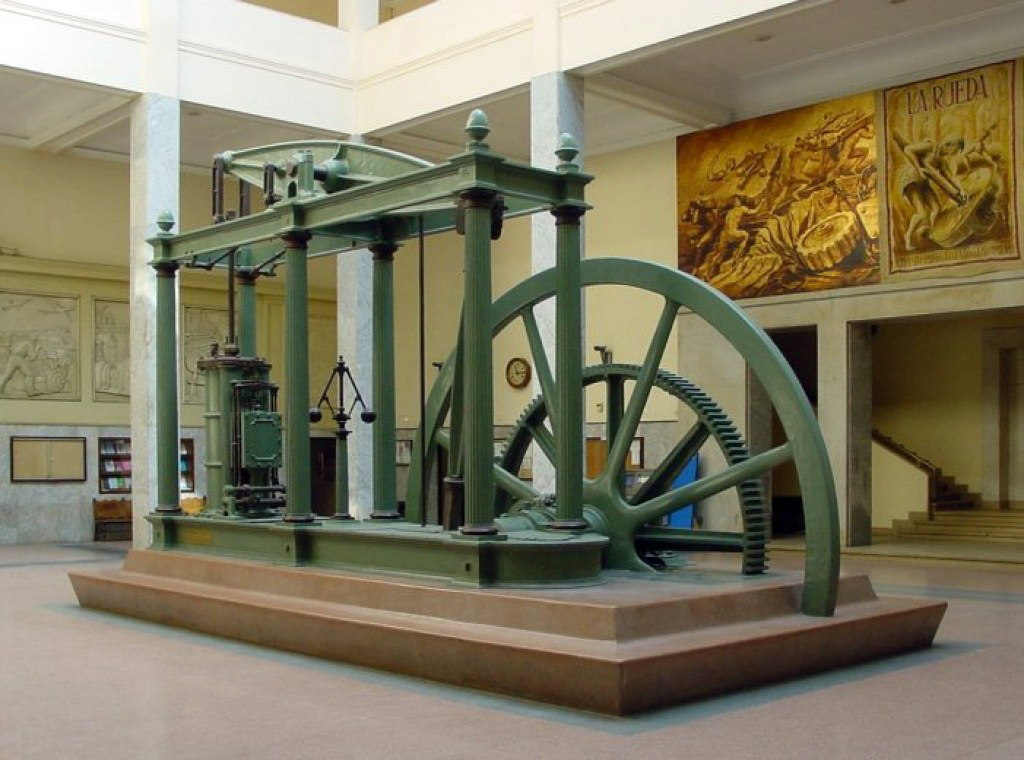
\includegraphics[width=0.5\textwidth]{Chapitre_1/Images/Maquina_vapor_Watt_ETSIIM.jpg}
    \caption{Watt steam machine\cite{Watt}}
    \label{fig:Watt}
\end{figure}

Then, later in the 18th century, the British James Watt (1736 - 1819) invented and commercialized a steam machine. Thanks to the great marketing around his product, the machine was very successful among the merchants. Indeed, at this time many machines were powered by horses.\\

James Watt saw this as an opportunity by creating a unit to compare its machines to the horses. The name of the unit was the horse power. Later the power will be expressed in Watt (W) in tribute to James Watt. One of the machines built by Watt is depicted on the Figure \ref{fig:Watt}.

This progressively leads to the implementation of the steam machines in Europe, and it was one of the most important elements of the Industrial Revolution. Indeed, aside the progressive replacement of the horses, wind and water mills also started to be replaced by mills powered by steam. At the beginning of the 19th, other fields like mining or merchandise transportation also started to utilize the steam machine technology as well.

In 1872, the American George Brayton (1830 - 1892) proposed the Brayton cycle as a ''reciprocating oil-burning engine'' \cite{Boles2006}. His engine consisted of a large cylinder where the compression, the combustion and, the expansion of the gas were successively performed. 

Nowadays, the Brayton cycle is used for gas turbines where the compression and expansion takes place in rotating machinery, also called turbomachine. Basically, the Brayton cycle is composed of three parts. 

First the compressor that will compress the ambient air to some pressure level. Then, there is a combustion chamber that will heat up the air to augment its level of energy. This heating-up is performed thanks to the injection of fuel into the combustion chamber. Finally, the resulting gas from the combustion is expanded into a turbine. The power produced by the expansion is partly consumed by the compressor while the rest is used to feed any kind of power receiver. The expanded gas is then released to the atmosphere. This cycle is depicted in the Figure \ref{fig:C1_GT} where the receiver is an electrical generator.

\begin{figure}[h]
    \centering
    \includegraphics[scale = 0.15]{Chapitre_1/Images/GT.png}
    \caption{Brayton gas cycle}
    \label{fig:C1_GT}
\end{figure}
There exists many variants of the Brayton gas cycles. The one proposed above is the simplest one where the air goes through a compressor, a combustion chamber and a turbine before returning to the environment. 

Variants are Brayton cycle where heat exchangers are used to recover heat when it is possible, or cycles where the compression and the expansion can be split into multiple stages, etc.

All these variants have been thought to solve problems encounter and to enlarge the range of possible applications where the Brayton gas cycle can be used. For instance, Brayton cycle is used in aircraft for the propulsion, or are integrated within a power plant to produce electricity.\\

This work is focused on the improvement of a computer code made by the company MITIS SA which aims to assess the performance of a multiple configuration of the micro gas turbine characterized by small component. While some additions to the program are done to increase its modularity, the main improvements are ones that will allow the computer code to utilize experimental results to increase its accuracy. \\

Not all the possible improvements will be considered for this master thesis. The main concern will be on the turbomachine and how to simulate the influence of the operating conditions on their performances based on performance maps. These maps can be considered as the footprint of each turbomachine.  The purpose will be to be able to easily modify the program by switching from one map to another one. Also, the integration of performance maps will give the ability to see the impact of the rotational speed of the compressor and turbine on their respective behaviors.



\newpage
%%%%%%%%%%%%%%%%%%%%%%%%%%%%%%%%
% Chapitre 2:                 %%
% Notion of thermodynamics    %%
%%%%%%%%%%%%%%%%%%%%%%%%%%%%%%%%
\graphicspath{{Chapitre_2/Images/}}
\chapter{Notions of thermodynamics}\label{C2}
%%%%%%%%%%%%%%%%%%%%%%%%%%%%%%%%%%%
%%%%%                         %%%%%
%%%%% Introduction chapitre 2 %%%%%
%%%%%                         %%%%%
%%%%%%%%%%%%%%%%%%%%%%%%%%%%%%%%%%%
\quad\, The principle and uses of the Brayton cycle have been discussed in the introduction. As explained, this concept has been applied for many usages, including electricity production and aircraft propulsion which are the most common and known applications. It has been exposed that from the invention proposed by George Brayton in the end of the 19th century, the technology did really evolve.

Indeed, the Brayton cycle engine first appears as a  piston engine where the compression, combustion and expansion occur in the same enclosure. Nowadays, the process is shared between at least three components (namely the compressor, the turbine and the combustion chamber).

However, the key notions to understand how theses components behave have not been introduced yet. This problematic will be covered by this chapter, which will introduce step-by-step those notions.
\section{Open/closed system}\label{sect:C2_Sys}
\quad\,  The thermodynamic is a science that ''studies the exchange of energy between a system and its environment or surroundings'' \cite{thermoApp_1}.
The system is defined as being the area of the space selected for the study. Between the system and the environment lies the boundary. This boundary can either be real or fictitious and can be static or mobile.

When the system is characterized, it has to be defined if it is an open or a closed system.

On one hand, closed systems do not exchange matter with the environment. Those systems are characterized by a control mass well delimited in the space of study. Therefore, only heat or work can be transferred from the system to the surroundings.

On the other hand, the open systems are ones where an arbitrary control volume well demarcated in the space is studied. In contrast to closed systems, open systems not only exchange work and heat with the environment, but also matter. Typical examples are the combustion chamber, heat exchanger, turbomachines, piping,...

\section{State functions and variables}\label{sect:C2_State}
\quad\, Let considered a system as defined in the previous section. The state functions are defined as ''a property of the system that only depends on its current state.” These functions are independent of the past of the system and describe the equilibrium state of the system.

When the state functions can be measured (directly or indirectly), these are called state variables. For example, the pressure $p$, the temperature $T$ or the volume $\mathrm{V}$ is state variables.

In this work, the units used for the state and function variables follow the international system (SI) of units \cite{Nist}. 
\subsection{Pressure}
\quad\, The pressure unit is the Pascal (Pa). 1 Pa corresponds to 1 N/m$^2$, where 1 N (kg$\cdot$m/s$^2$) is the required force to increase each second by 1 m/s the velocity of a body of 1 kg.

The pressure is also often expressed in bar. 1 bar corresponding to 1e5 Pa.
\subsection{Temperature}
\quad\, The temperature unit is the Kelvin (K). 273.15\degree K corresponds to 0\degree C, temperature at which pure water starts freezing.
\subsection{Volume}
\quad\, The volume unit is the meter cube (m$^3$).
\section{Ideal gas equation}
\quad\, It can be shown that the equilibrium state of a system can be described by those three variables. Also, among $p$,  $T$ and $\mathrm{V}$, only two of them are independent. 

This means that a state relation defined as \textbf{F}($p$, $T$, $\mathrm{V}$)= 0.

For the ideal gas, the most well-known state relation is the relation of perfect gases defined in (\ref{eq:C2_GP}).

\begin{align}
\setstretch{1}
p\cdot \mathrm{V} &= m\cdot\frac{R}{MM}\cdot T\nonumber\\
p\cdot \mathrm{v} &= r\cdot T\label{eq:C2_GP}    
\end{align}
Where \textit{m} is the quantity of matter (kg), $R=8.314$ J/mole$\cdot$K is the universal gas constant, $\mathrm{v}$ the specific volume (m$^3$/kg) and $MM$ is the molar mass (kg/mole\footnote{Where one mole corresponds to $\sim 6\cdot 10^{23}$ elementary entities (atoms, molecules,...)}) of the system. 

The density $\rho$ of the gas is given as being one over the specific volume $\mathrm{v}$.
\section{Energy}\label{sect:C2_Ener}
\quad\, In the subsection \ref{sect:C2_Sys}, the notion of energy has been mentioned without characterizing it beforehand. From the first principle of the thermodynamic, it is stated that the energy cannot be created nor destroyed. Therefore, it can only be converted, meaning that the energy exists into multiple forms (thermal, mechanical, electrical,...)\cite{thermoApp_2}. 

The unit of the energy is the Joule (J), and the sum of all the energies in a system is called the total energy $E$. 1 Joule corresponds to the work required to move a body over 1 meter using a force of 1 N.

The energy is a state variable. This implies that this quantity allows characterizing the state of the system. When considering the energy, its absolute value is not something that is defined. Instead, the energy is always computed based on a reference value. Since the interest is often in the variation of the energy, the chosen reference value does not really matter.

Considering the variation of the total energy from a state \textbf{1} to a state \textbf{2}, it is obtained that the total energy variation is equal to the sum of the variation of the internal, kinetic and potential energy $U$, $KE$ and $PE$ (respectively). The internal energy $U$ corresponds to the sum of all the ''microscopic'' energy within the system.  

Thus, the definition of the total energy variation is given in the relation (\ref{eq:C2_E}).

\begin{equation}
\setstretch{1}
    \Delta E = \Delta U + \Delta KE + \Delta PE \label{eq:C2_E}
\end{equation}
\begin{align*}
\setstretch{1}
    \text{with } \Delta U  &= U_2 - U_1 =  m\cdot(u_2 - u_1) \text{: Variation of the internal energy}\\
                 \Delta KE &= \frac{1}{2}m\cdot(v^2_2 - v^2_1)\text{: Variation of the kinetic energy}\\
                 \Delta PE &= m\cdot \text{g}\cdot(z_2 - z_1)\text{: Variation of the potential energy}
\end{align*} 
Where $\text{g}=9.81$ m/s$^2$ is the standard gravity, $z$ is the altitude of the system position (m), $v$ is the velocity of the fluid (m/s) and $u$ is the specific internal energy (J/kg).


In the subsection \ref{sect:C2_Sys}, it has been said that any system exchange energy with the surroundings as heat and work. The heat is defined as ''the form of energy which is exchanged between the system and its environment when there is a gradient of temperature between these two entities.'' 

As the heat is always referred as a heat flux between two bodies, the phenomenon is called heat transfer. There exist three modes of heat transfer which are namely the

 
\begin{itemize}
\setstretch{1}
    \item conduction: Heat transfer through a non-flowing material due to the interaction of ''molecular scale energy carriers within the material''\cite{GregoryNellis2015}
    \item convection: More complex conduction when considering a flowing fluid.
    \item radiation: The heat is transferred as electromagnetic waves.
\end{itemize}
The heat transfer is denoted $Q$. A system that does not exchange heat with the surroundings is called an \textbf{adiabatic} system.

Aside the heat transfer, the system can also exchange energy by producing a work. The work $W$ is ''the form of energy exchanged associated to a force applied over a certain distance''. 

The work is exchanged if the force applied to the system creates a displacement of its boundary. By extension to the definition of the work, the power generated by a system is defined as the work per unit of time and is expressed in Watt (or W).

Both the heat transfer and work are called ''path functions'' because they are both linked to the evolution of a system and not to the state of this system. Indeed, there isn't any guarantee that the work or the heat transfer exchanged during a transformation and its inverse will be identical.
Thus, these are not thermodynamic variables (like the temperature or the pressure).
\subsection{Energy balance}
\quad\, It has been previously mentioned several mechanisms to exchange energy from the system to its environment. Aside from the heat transfer and the work transfer, the energy can also be exchanged using mass transfer. 

Indeed, if the system is open, the mass entering and exiting the system will convey energy. To recall the first principle of the thermodynamic, the energy cannot be created or destroyed. 

Based on the statement, the energy balance of the system is given by the following generic formulation (\ref{eq:C2_EB}).
\begin{equation}
\setstretch{1}
    E_{in} - E_{out} = (Q_{in} - Q_{out}) + (W_{in} - W_{out}) + (E_{mass,in} - E_{mass,out}) = \Delta E_{system} \label{eq:C2_EB}
\end{equation}
With $E_{mass}$ the energy conveys by the mass entering/exiting the system.

It is possible to write a temporal formulation (\ref{eq:C2_PB}) of the energy balance named \textbf{power balance}.  
\begin{equation}
\setstretch{1}
    \dot{E}_{in} - \dot{E}_{out} = (\dot{Q}_{in} - \dot{Q}_{out}) + (\dot{W}_{in} - \dot{W}_{out}) + (\dot{E}_{mass,in} - \dot{E}_{mass,out}) = \frac{dE_{system}}{dt} \label{eq:C2_PB}
\end{equation}
With $\frac{dE_{system}}{dt}=0$ for a system where the variation of energy does not change in the time.
\subsection{Energy conservation efficiency}
\quad\, When the system is transferring or converting energy, it is often interesting to quantify the quality of this transfer/conversion. The efficiency is defined to provide this quantification, and its definition is the
$\frac{\text{Desired ouptut}}{\text{Required input}}$. 

For example, a electric heater with the efficiency of 90\% is a system such that 90\% of the electrical energy consumed is converted into thermal energy .  
Considering the combustion of fuel, the combustion efficiency is defined as the ratio
$$ \eta_{cc} = \frac{\dot{Q}}{\dot{m}_{fuel}\cdot HCV_{fuel}}$$
Where $\dot{m}_{fuel}$  and $HCV_{fuel}$ is the mass flow rate of fuel and the heating calorific value of the fuel injected into the combustion chamber.

\section{Phases}
\quad\ When a system is considered, the transformations that the system will see are usually applied to a fluid or a solid material. These elements are characterized by its level internal of energy and the surrounding conditions.

The phase of an element is defined based on the arrangement of the molecules constituting the elements. There exists three different types of phases:

\begin{itemize}
    \setstretch{1}
    \item Gas: The spacing between the molecules is large and the molecules are disordered. Each molecule is free to move within the gas in every direction.
    \item Liquid: There is an internal order within the liquid. The displacement of the molecules is limited to the translation and the rotation. The distance between each molecule is smaller than for the gas.
    \item Solid: The order is perfect. The molecules can only vibrate around their respective anchor point, and the distance between each molecule is a little bit smaller than for the liquid.
\end{itemize}

The three phases are illustrated in the Figures \ref{fig:C2_gas}, \ref{fig:C2_liq} and  \ref{fig:C2_sol}.

\begin{figure}[h]
     \centering
     \begin{subfigure}[b]{0.3\textwidth}
         \centering
         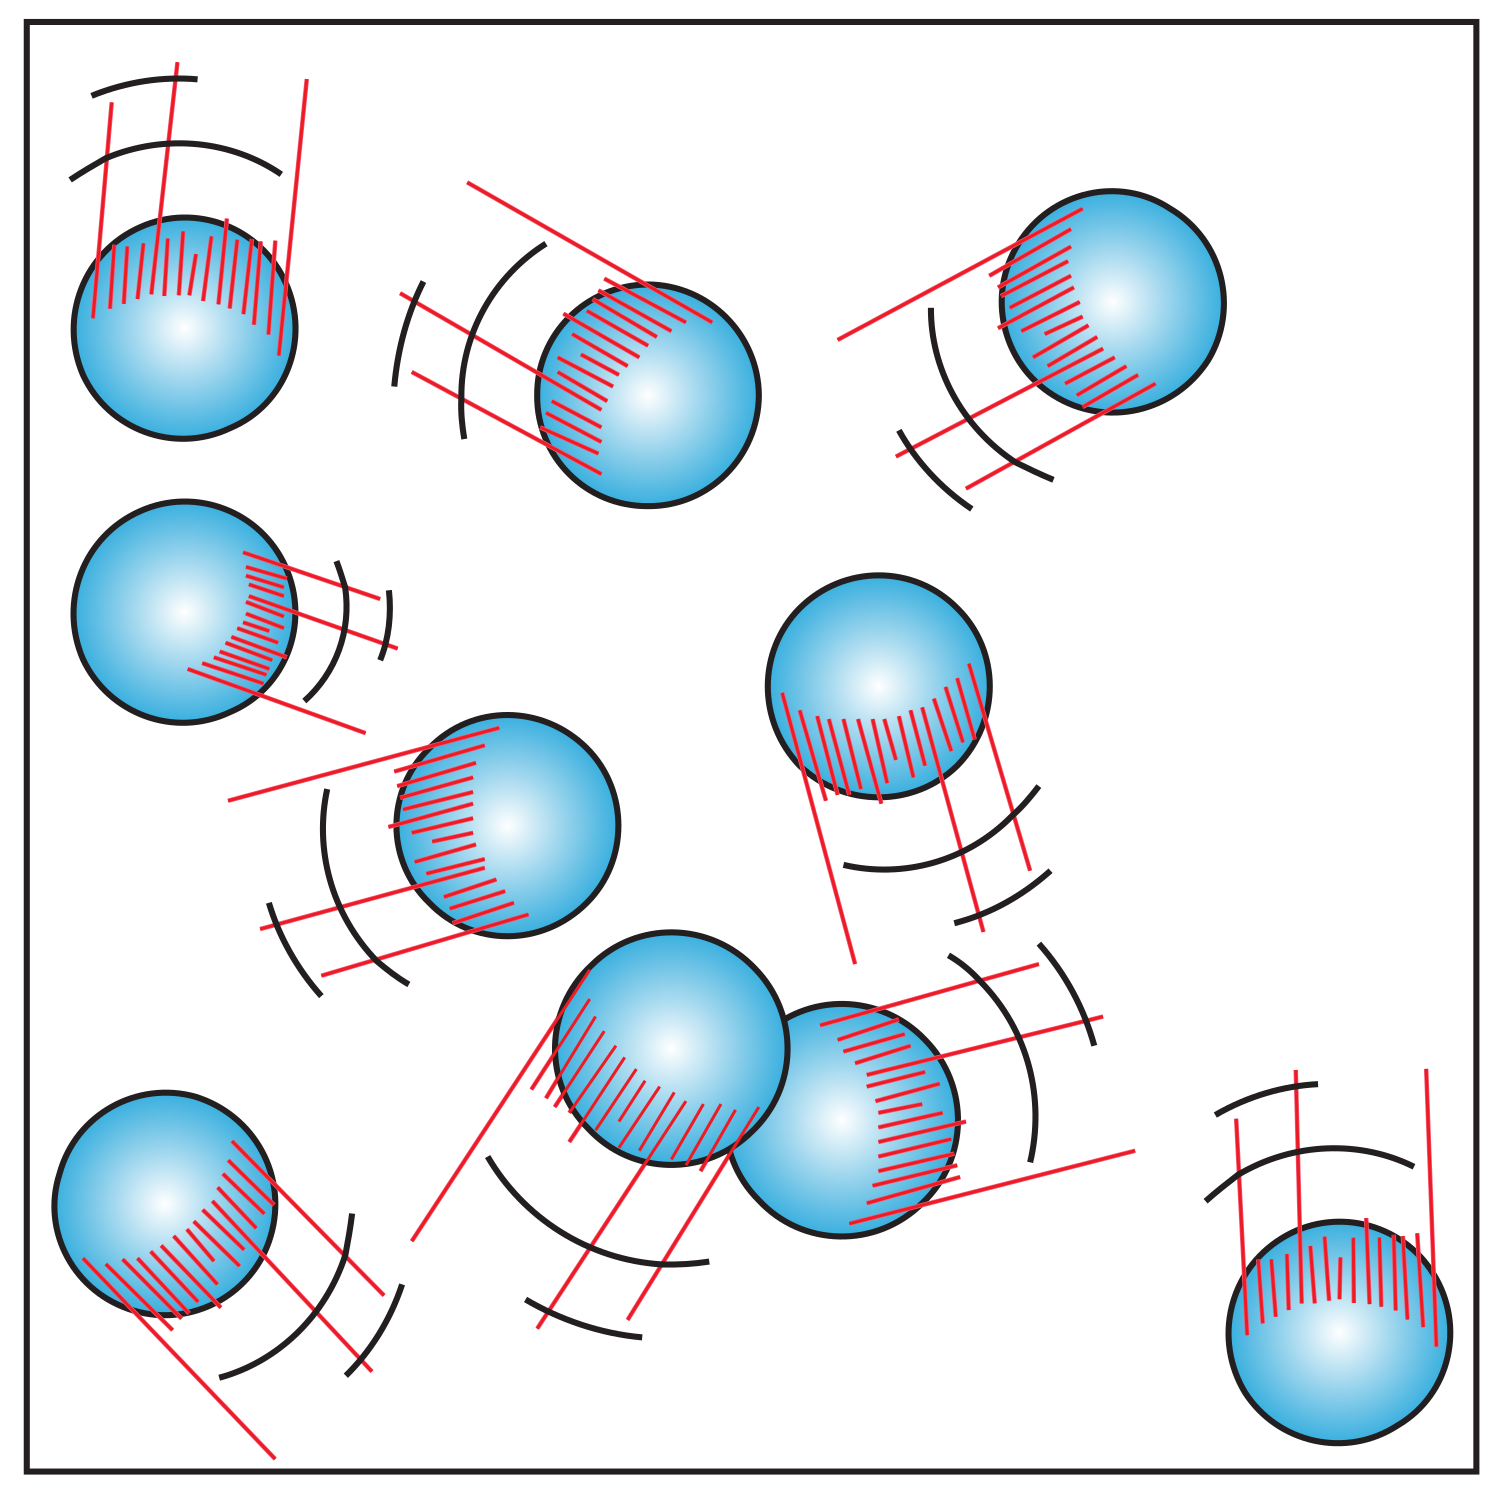
\includegraphics[width=\textwidth]{Chapitre_2/Images/gas.png}
         \caption{Gas.}
         \label{fig:C2_gas}
     \end{subfigure}
     \begin{subfigure}[b]{0.3\textwidth}
         \centering
         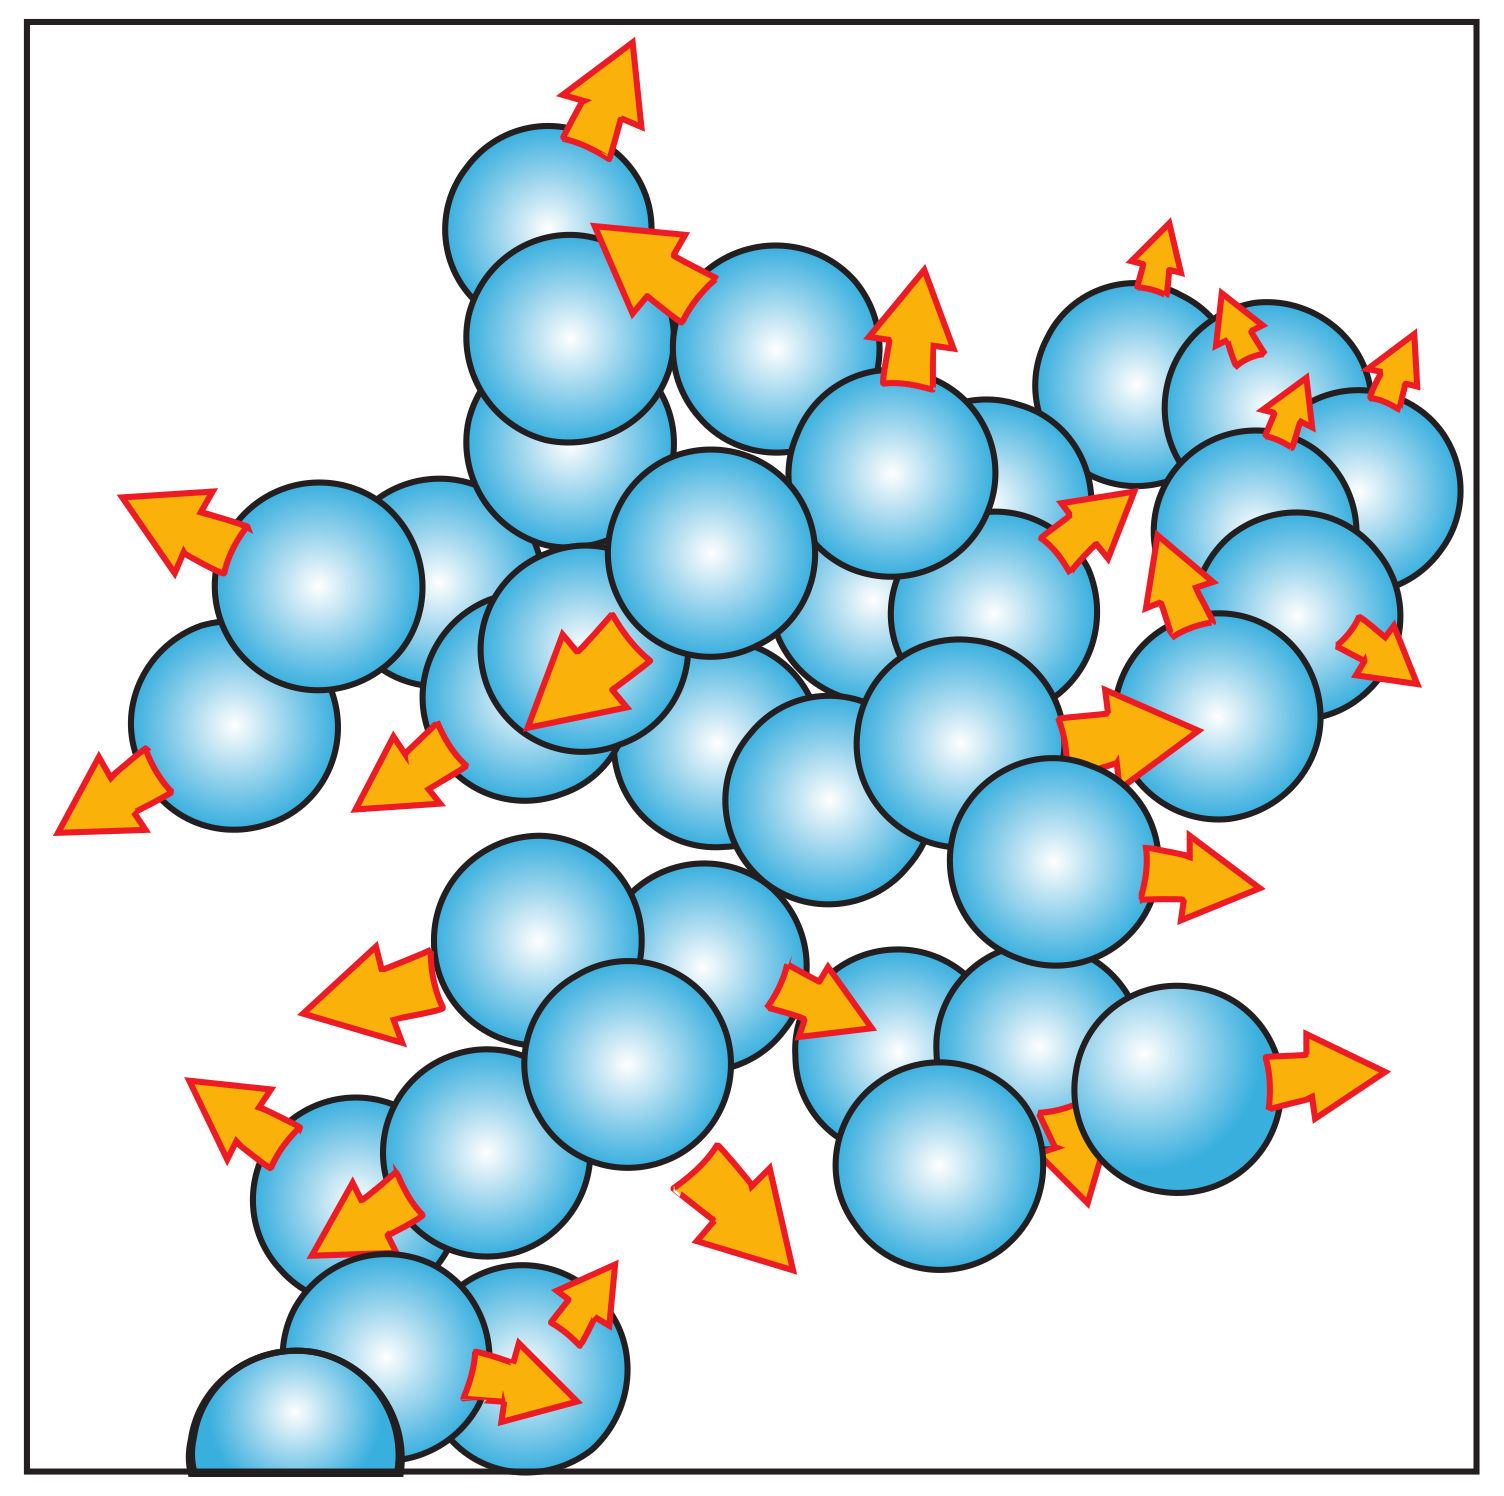
\includegraphics[width=\textwidth]{Chapitre_2/Images/liquid.png}
         \caption{Liquid.}
         \label{fig:C2_liq}
     \end{subfigure}
     \begin{subfigure}[b]{0.3\textwidth}
         \centering
         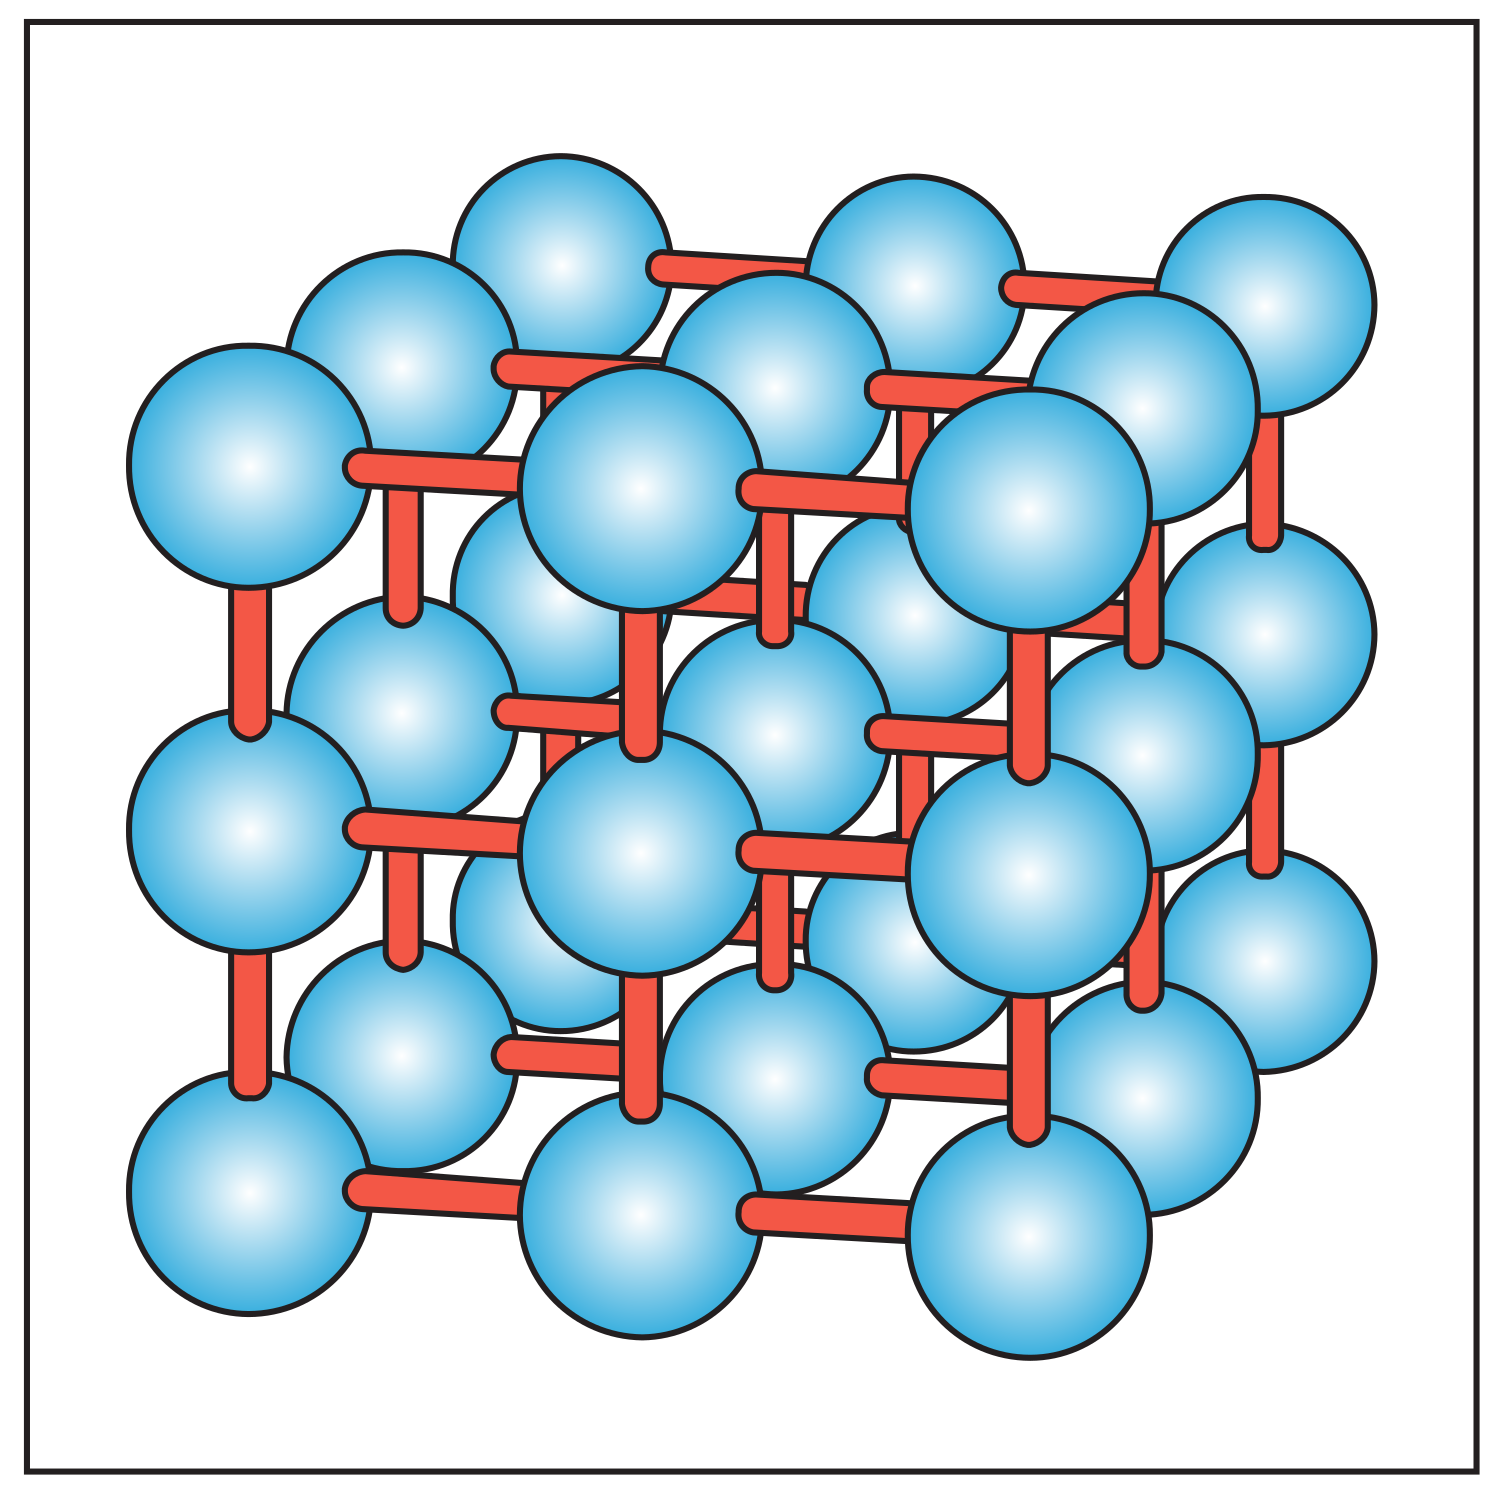
\includegraphics[width=\textwidth]{Chapitre_2/Images/solid.png}
         \caption{Solid.}
         \label{fig:C2_sol}
     \end{subfigure}
        \caption{Arrangement of the molecules depending on the phases\cite{Boles2006}.}
        \label{fig:C2_phase}
\end{figure}

The phase of a given fluid is determined by its level of energy and the surrounding conditions. When there is a transition from one phase to the other, the two phases are coexisting during the transition.


\newpage
%%%%%%%%%%%%%%%%%%%%%%%%%%%%%%%%%
%% Chapitre 3:                 %%
%% Principles of thermodynamics%%
%%%%%%%%%%%%%%%%%%%%%%%%%%%%%%%%%
\graphicspath{{Chapitre_3/Images/}}
\chapter{Principles of thermodynamics}\label{C3}
%%%%%%%%%%%%%%%%%%%%%%%%%%%%%%%%%%%
%%%%%                         %%%%%
%%%%%Introduction chapitre 2_5%%%%%
%%%%%                         %%%%%
%%%%%%%%%%%%%%%%%%%%%%%%%%%%%%%%%%%
\quad\ The previous chapter covered many concepts to start analyzing a thermodynamic system submitted to various transformations. Among those, the notion of state variables defining the equilibrium state of such system has been defined. 

This chapter will use the first and second principles of the thermodynamic to introduce some state variables that will be used when studying a thermodynamic cycle. Also, a classification of the different transformations will be established.
\section{First principle}
\quad\ The first principle of thermodynamics state that the energy cannot be created or destroyed, but is rather converted from one form to another.
The chapter \ref{C2} shows that for the general case, (\ref{eq:C3_EB}) gives a generic formulation for the energy balance of a system. 

\begin{equation}
  \setstretch{1}
  E_{in} - E_{out} = (Q_{in} - Q_{out}) + (W_{in} - W_{out}) + (E_{mass,in} - E_{mass,out}) = \Delta E_{system} \label{eq:C3_EB}
\end{equation}
\subsection{Enthalpy}
\quad\ Considering a closed system, the third term of the energy balance is nullified. Thus, the variation of the total energy from a state \textbf{1} to a state \textbf{2} is given in the relation \ref{eq:C3_EBC}.

\begin{equation}
\setstretch{1}
E_{2} - E_{1} = Q_{1-2} - W_{1-2} = m\cdot\left(u_2 - u_1\right) + \frac{1}{2}m\cdot\left(v^2_2 - v^2_1\right) + m\cdot g\cdot\left(z_2 - z_1\right)\citep{Dewallef2019} \label{eq:C3_EBC}
\end{equation}
Let’s note that the terms of kinetic and potential energy are often negligible compared to the internal energy. Thus, the last two terms are supposed equal to zero for the remaining of the derivations.\newpage

The relation (\ref{eq:C3_EBC}) can be adapted to be applied for the open system by introducing an accumulation term $\Delta E_{cv}$. This correction allows the formulation (\ref{eq:C3_EBO}) of the energy balance.

\begin{equation}
\setstretch{1}
Q_{1-2} - W_{1-2} - E_{2} - E_{1} = \Delta E_{cv}\label{eq:C3_EBO}
\end{equation}

\begin{figure}[h]
\centering
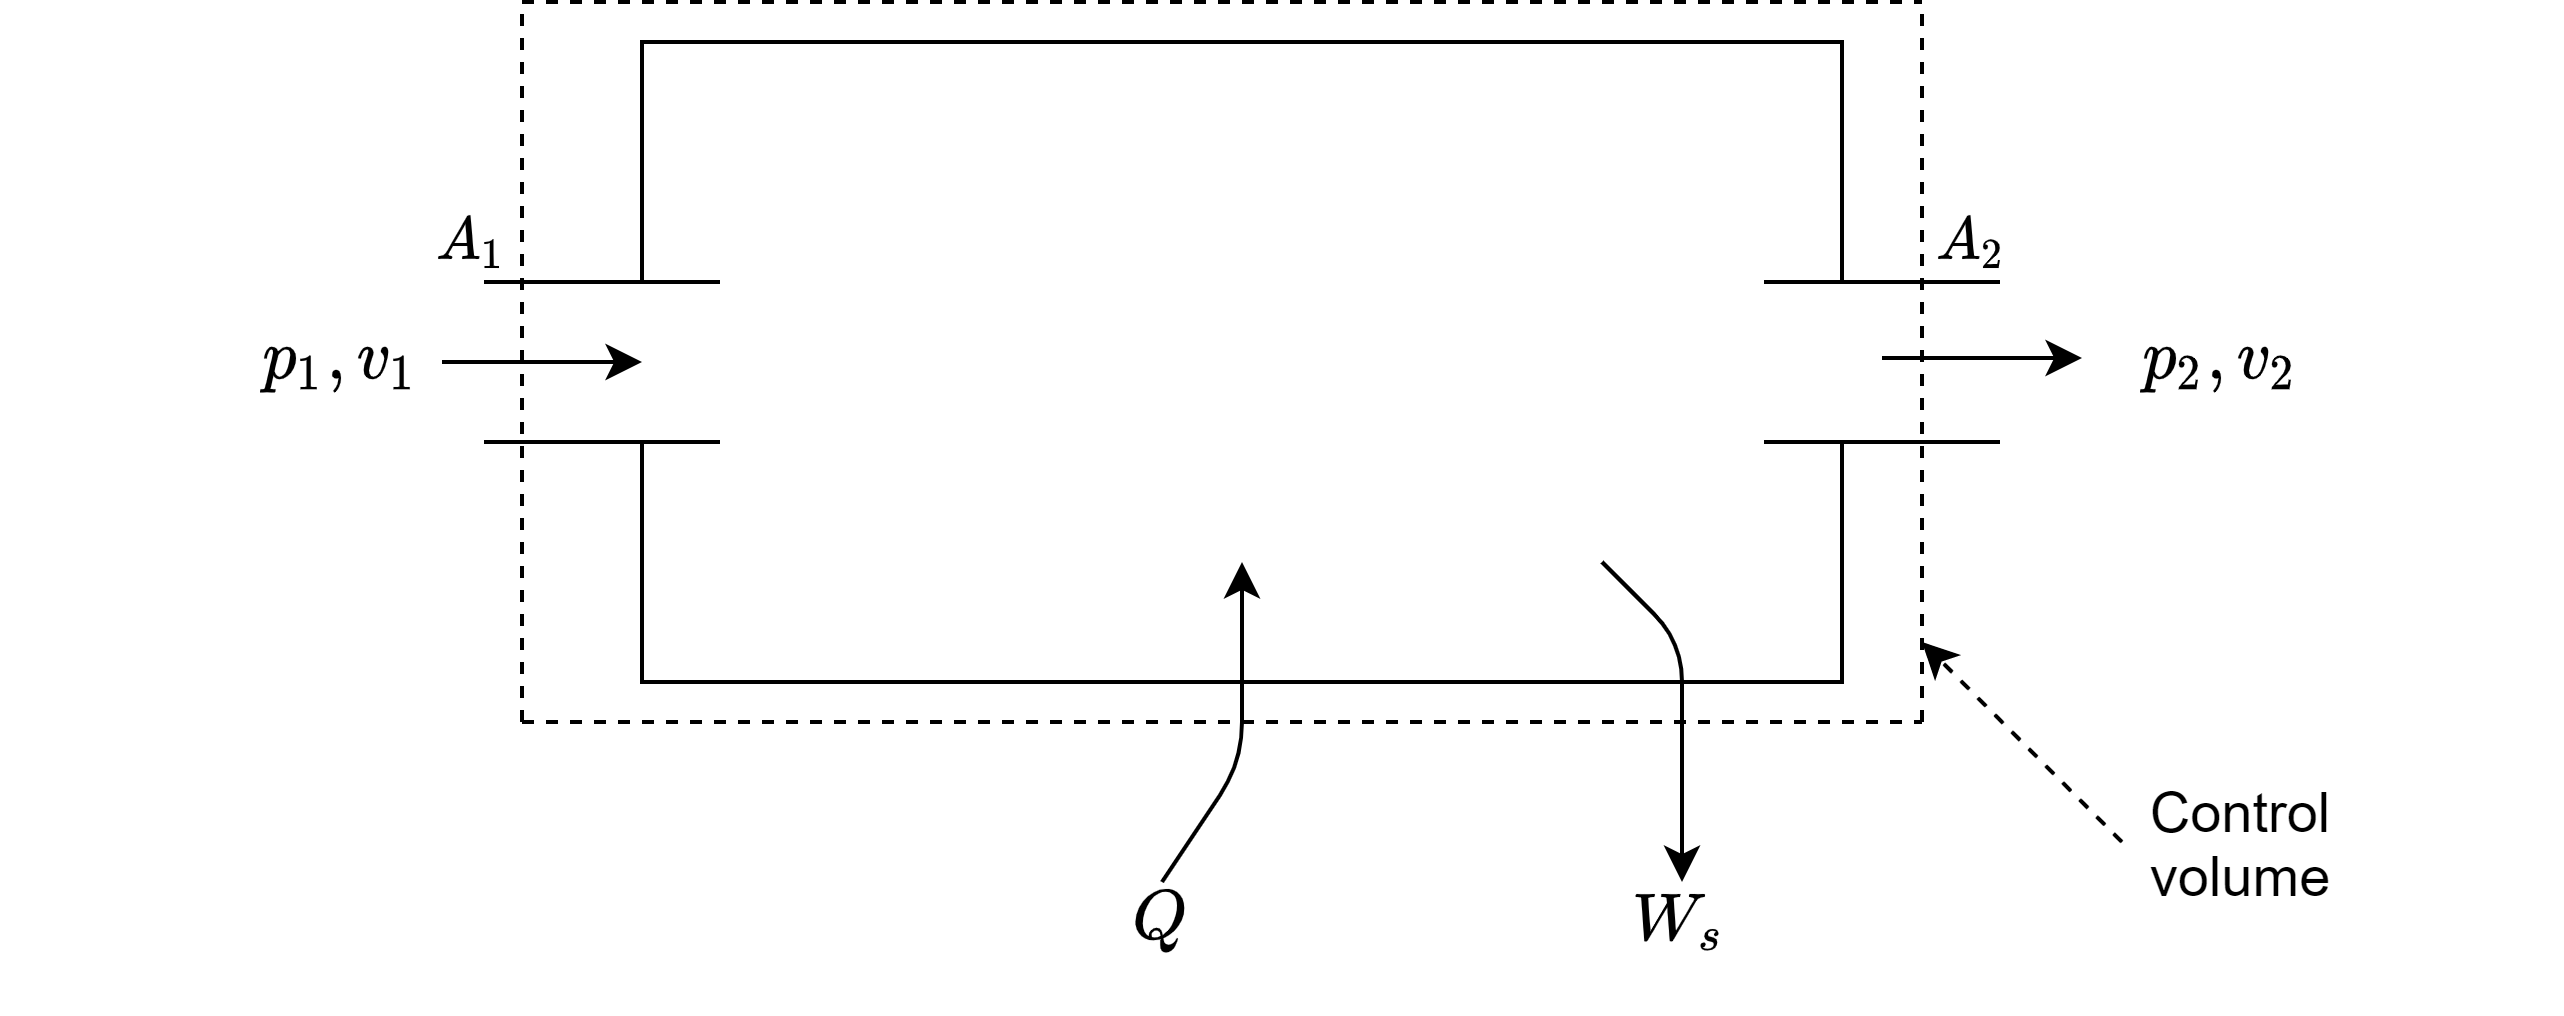
\includegraphics[width=0.7\textwidth]{control_volume.png}
\caption{System control volume.}
\label{fig:C3_VC}
\end{figure}
The Figure \ref{fig:C3_VC} depicts an open system with an inlet and outlet area $A_1$ and $A_2$ respectively. The work $W$ for this system is defined by the equality (\ref{eq:C3_work}).

\begin{equation}
\setstretch{1}
W = p_2\cdot A_2\cdot v_2\cdot \Delta t - p_1\cdot A_1\cdot v_1\cdot \Delta t + W_s \label{eq:C3_work}
\end{equation}      
Where $p$ and $v$ are the pressure and the velocity.

If it is supposed that there is no accumulation of matter in the system, the energy balance (\ref{eq:C3_EBC}) can be expressed as given in the relation (\ref{eq:C3_EBH}), taking into account the definition (\ref{eq:C3_work}) of the work $W$.

\begin{equation}
\setstretch{1}
q - w_s = u_2 +p_2\cdot \mathrm{v}_2 - u_1 - p_1\cdot \mathrm{v}_1 = h_2 - h_1\label{eq:C3_EBH}
\end{equation}
Where $q$, $w_s$, and $h$ are respectively the specific work, heat and \textbf{enthalpy} (J/kg).  

For the case of an ideal gas, the enthalpy and the internal energy only depend on the temperature $T$. Indeed, taking the relation (\ref{eq:C2_GP}) from the previous chapter, the relation (\ref{eq:C3_h}) can easily be deduced.
\begin{equation}
\setstretch{1}
h = u(T) + p\cdot \mathrm{v} = u(T) + r\cdot T \label{eq:C3_h}
\end{equation}
\subsection{Specific heat capacity}
\quad\ The previous subsection was meant to define the enthalpy. This state variable is used in place of the internal energy when dealing with an open system.

Another quantity that is useful for the study of a system is the \textbf{specific heat capacity}. This state variable is defined as the required energy to increase of 1\degree C the temperature of 1 kg of a substance. 
 
The required heat to produce this effect depends on the ways the transformation takes place. For a transformation under constant volume constraints, it is called specific heat capacity at constant volume and denoted $c_v$. If the transformation is performed at constant pressure, the symbol associated with the specific heat capacity is $c_p$.

It is worth noting that the specific heat capacity at constant pressure is always higher than the $c_v$. When performing the transformation at constant pressure, the gas expands against the external pressure. This means that the gas does work and, this is the reason behind the greater value of the supplied heat when dealing with a transformation at constant pressure. 

For an ideal gas, the variation of the internal energy can be linked to the specific heat capacity at constant volume as written in the relation (\ref{eq:C3_UC}).

\begin{equation}
\setstretch{1}
du = c_vdT \rightarrow u_2 - u_1 = \int_{T_1}^{T_2} c_vdT\label{eq:C3_UC}
\end{equation} 
Similarly, the variation of the enthalpy can be expressed using the specific heat capacity at constant pressure.

\begin{equation}
\setstretch{1}
dh = c_pdT \rightarrow h_2 - h_1 = \int_{T_1}^{T_2} c_pdT\label{eq:C3_UP}
\end{equation} 
These two relations, with the equality (\ref{eq:C3_h}), provide the required tools to express the gas constant $r$ as a function of the temperature only. 

\begin{equation}
\setstretch{1}
r = c_p - c_v \label{eq:C3_r}
\end{equation}

Aside the gas constant, the heat capacity ratio $k$ (\ref{eq:C3_k}) is also a useful variable to be computed.
\begin{equation}
\setstretch{1}
k = \frac{c_p}{c_v} \label{eq:C3_k}
\end{equation}
\subsection{Carnot cycle}
\quad\, In the previous subsections, the first principle of the thermodynamic was used to deduce two useful state variables, namely the enthalpy and the specific heat capacity.

Now, these new tools can be used to study the case where the transformation applied to a system is reversible. A necessary condition for the reversibility is that the transformation has to be done in quasi-equilibrium. This implies that if the transformation is reversed, the system goes back to its initial state. An example of an irreversible transformation is a transformation where a heat transfer is generated due to friction. 

\begin{figure}[h]
\centering
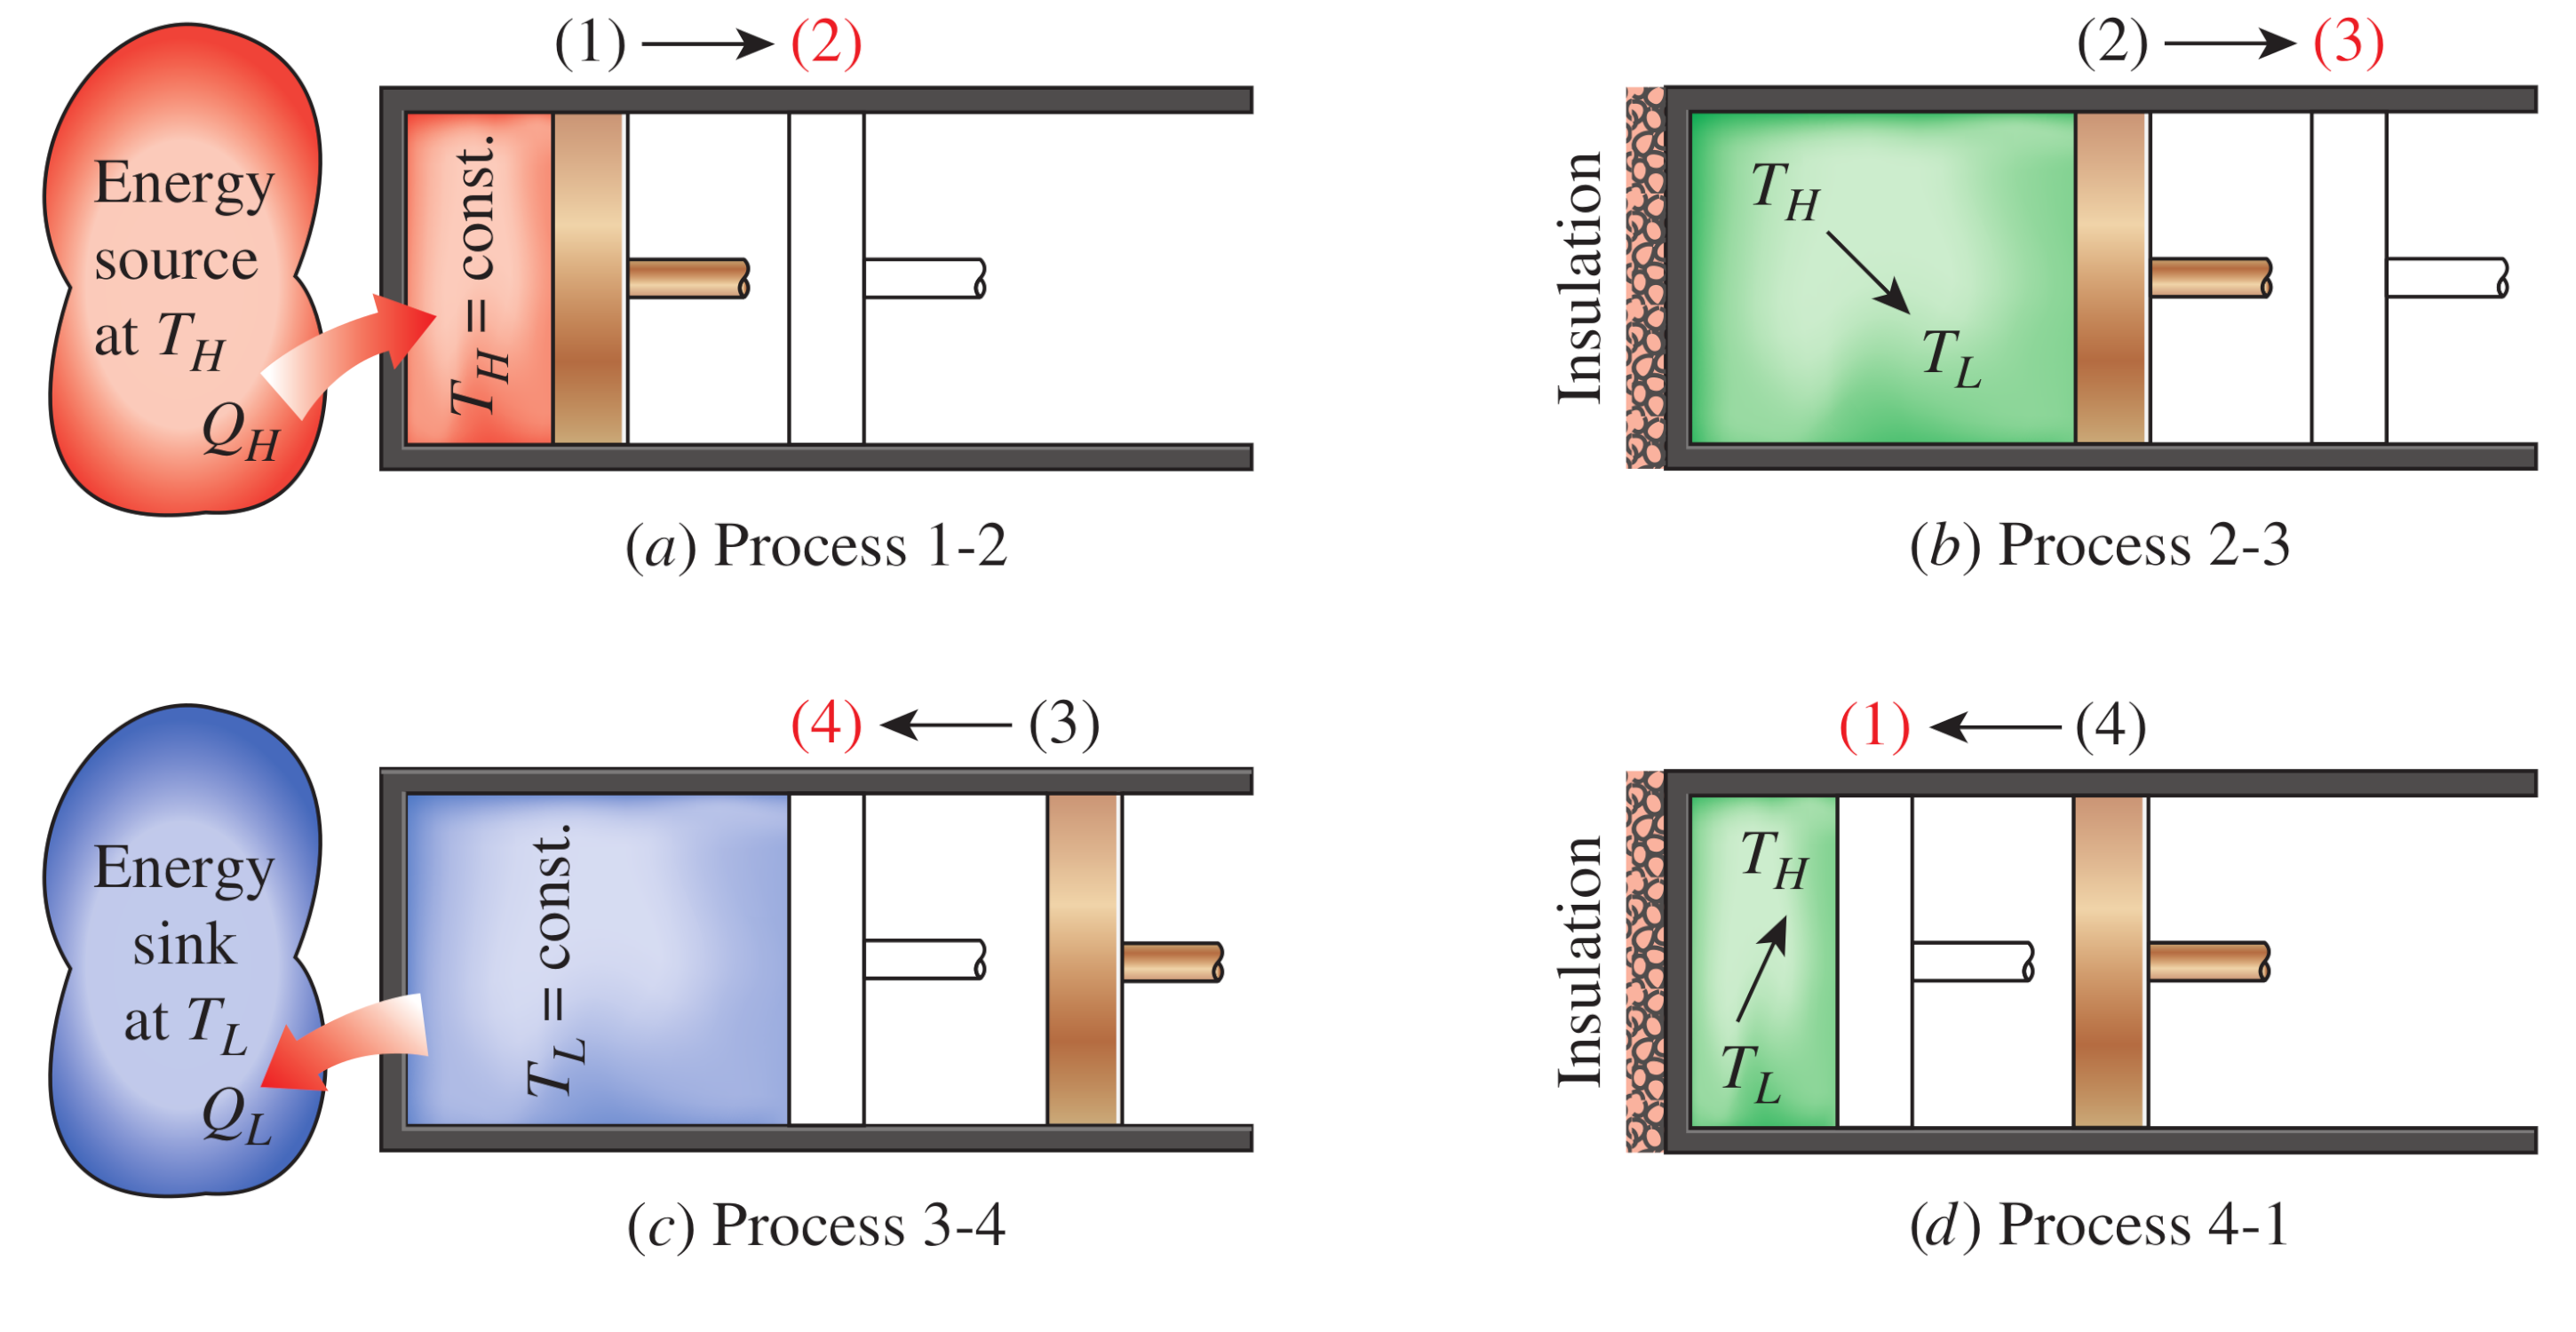
\includegraphics[width=0.7\textwidth]{Carnot_schema.png}
\caption{Carnot cycle - Schematic \cite{2015}.}
\label{fig:C3_Carnot}
\end{figure}

The Carnot cycle is a thermodynamic cycle composed of four reversible transformations illustrated in Figure \ref{fig:C3_Carnot}. The transformations are defined as follows.

\begin{itemize}
\setstretch{1}
\item \textbf{1} to \textbf{2} (Figure \ref{fig:C3_Carnot}a): Reversible isothermal expansion with a heat transfer $Q_H$ from the environment to the system
\item \textbf{2} to \textbf{3} (Figure \ref{fig:C3_Carnot}b): Reversible  adiabatic expansion
\item \textbf{3} to \textbf{4} (Figure \ref{fig:C3_Carnot}c): Reversible isothermal compression with a heat transfer $Q_L$ from the system to the environment
\item \textbf{4} to \textbf{1} (Figure \ref{fig:C3_Carnot}d): Reversible adiabatic compression
\end{itemize}
For visual representation, this cycle has been represented in the p-V diagram \ref{fig:C3_CarnotPV} where the different transformations are illustrated.

\begin{figure}[h]
\centering
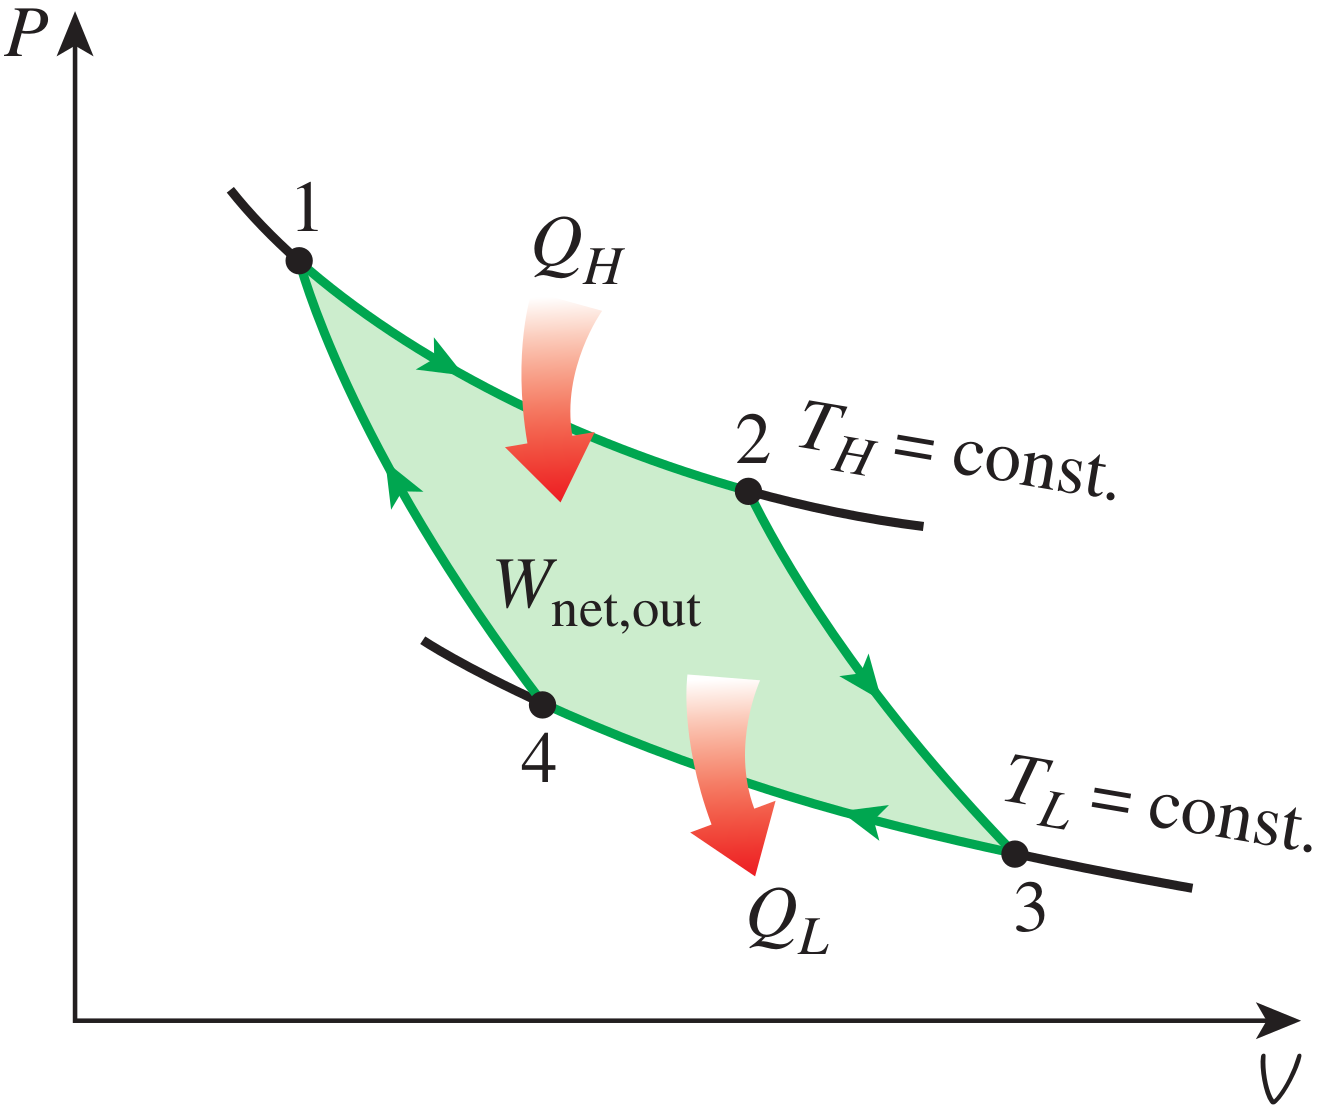
\includegraphics[width=0.5\textwidth]{Carnot_PV.png}
\caption{Carnot cycle - p-V diagram \cite{2015}.}
\label{fig:C3_CarnotPV}
\end{figure}
Using the first principle, the net work provided by the cycle is equal to $W_{net,out}=Q_H-Q_L$. From this result and the definition of the efficiency in chapter \ref{C2}, the efficiency of the Carnot cycle is given in (\ref{eq:C3_Carnoteff}).

\begin{equation}
\setstretch{1}
\eta_{carnot} = \frac{W_{net,out}}{Q_H} = 1 - \frac{Q_H}{Q_L}\label{eq:C3_Carnoteff}
\end{equation} 
Considering that the working fluid is an ideal gas, it can be demonstrated that the heats $Q_H$ and $Q_L$ can be replaced by the corresponding temperature $T_H$ of the hot source and $T_C$ of the cold sink.

\begin{equation}
\setstretch{1}
\eta_{carnot}=1-\frac{T_H}{T_L}\label{eq:C3_eff_carnot}
\end{equation} 
The efficiency of the Carnot cycle is optimal. This implies that for any system playing with a hot source $T_H$ and a cold sink $T_C$, its efficiency cannot be greater than the Carnot efficiency with the \textbf{same} hot source and cold sink temperatures.
\subsection{Entropy}
\quad\ The last lines explained that a system with a hot source $T_H$ and a cold sink $T_C$ will never have an efficiency greater than the Carnot efficiency (for the same source and sink).

It has been demonstrated in 1865 by the German physicist R. J. E. Clausius that "the cyclic integral $\oint\frac{\delta Q}{T}$ is always less than or equal to zero."\cite{2015}

\begin{equation}
\setstretch{1}
\oint\frac{\delta Q}{T} = \frac{Q_H}{T_H} - \frac{Q_L}{T_L}\leq 0\label{eq:C3_cyc}
\end{equation}
For the Carnot cycle, the integral is equal to zeros because the two ratios $\frac{Q_H}{Q_L}$ and $\frac{T_H}{T_L}$ are equal.
From the definition (\ref{eq:C3_cyc}), it can be defined a new state variable named \textbf{entropy}. The entropy $s$ is always measured based on a reference point, and its expression is given in the relation (\ref{eq:C3_S}).

\begin{equation}
\setstretch{1}
ds \triangleq \frac{\delta Q_{rev}}{T}\label{eq:C3_S}
\end{equation}
Where $\delta Q_{rev}$ is the "infinitesimal quantity of heat exchanged in a reversible way between the system and the environment at the temperature T."\cite{Dewallef2019} 

For a reversible adiabatic transformation, the $\delta Q_{rev}=0$. This implies that the entropy remains constant. Such transformations are called \textbf{isentropic} transformation.
\begin{figure}[h]
\centering
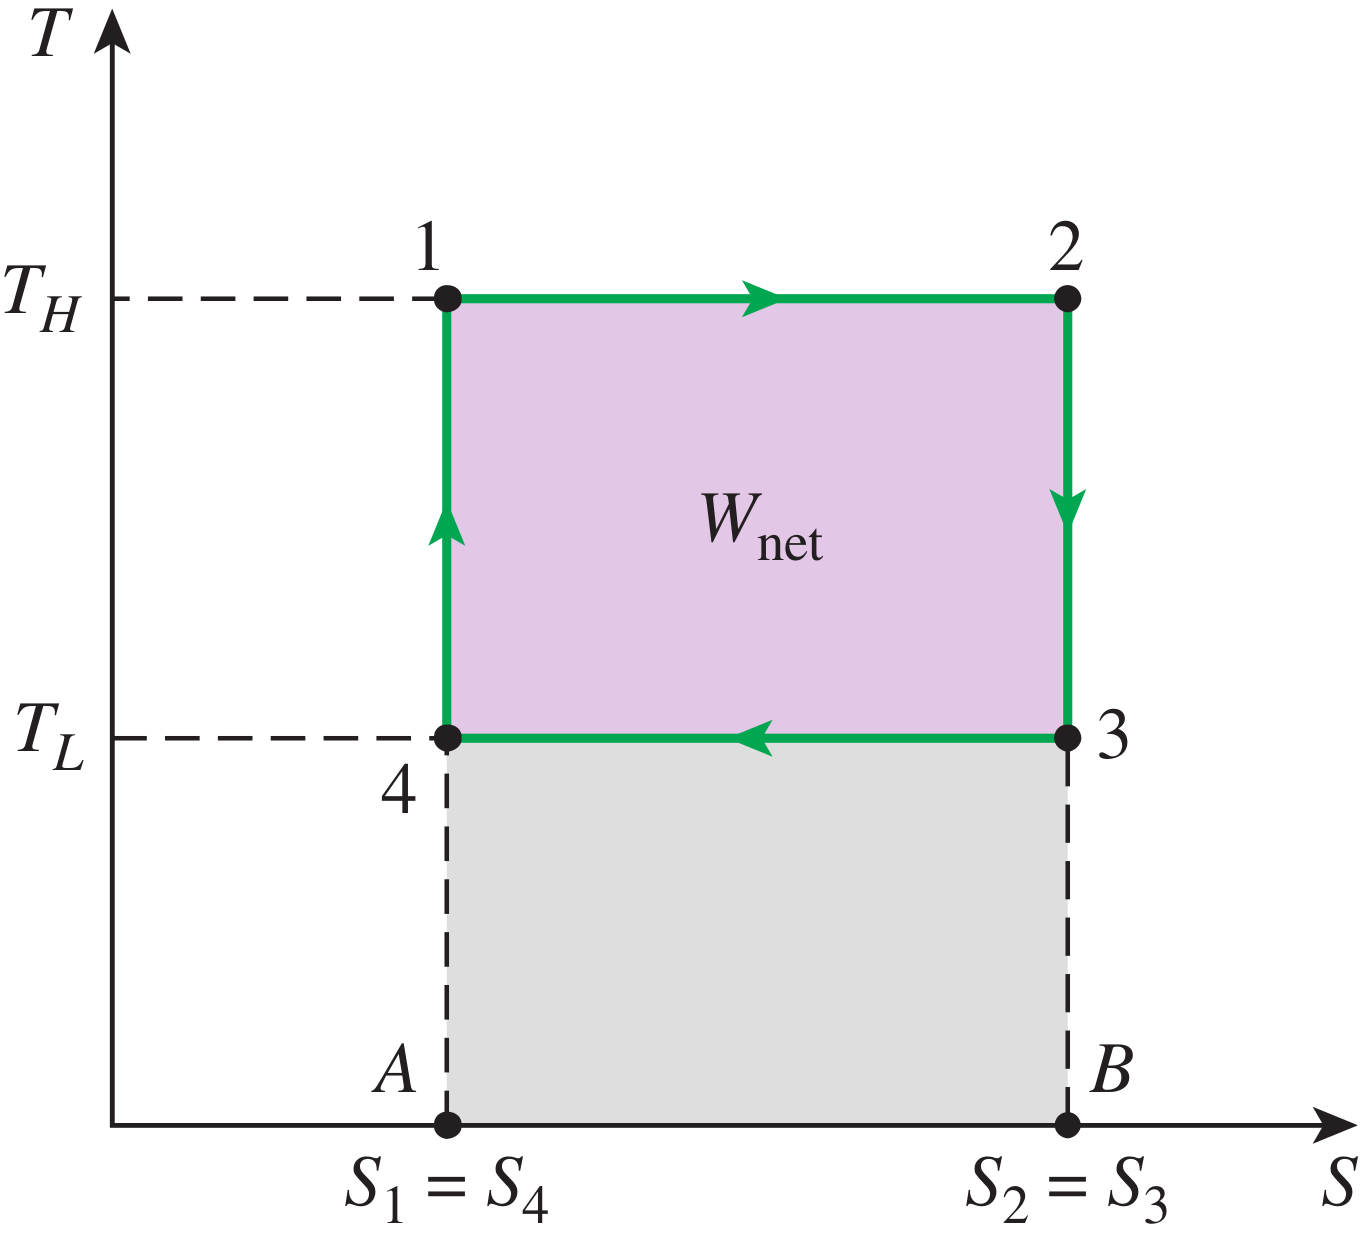
\includegraphics[width=0.5\textwidth]{Carnot_TS.png}
\caption{Carnot cycle - T-s diagram \cite{2015}.}
\label{fig:C3_CarnotTS}
\end{figure}
\section{Second principle}
\quad\, Defining the entropy gives a great tool to measure the "quality" of the transformation compared to a similar but reversible transformation.

Based on this definition, one formulation of the second principle of the thermodynamic is that for every transformation, the entropy of the final state of any isolated system is greater or equal to the one of the initial state.

Considering the system defined in the previous lines, it can be said that the increase of entropy $\Delta s_L$ of the cold sink has to be at least greater than the diminution of entropy $\Delta s_H$ of the hot source.

In the case of the Carnot cycle, both variations are equal. This is illustrated on the T-s diagram \ref{fig:C3_CarnotTS} where the entropy of states \textbf{1} and \textbf{2} are respectively equal to the entropy of states \textbf{4} and \textbf{3}.
\section{Type of transformations}
\quad\ During this chapter, it has been mentioned several times the notions of reversible processes. 

As it has been explained, a transformation is said reversible if it takes an infinite amount of time to bring the system from its initial state \textbf{1} to its final state \textbf{2}. The different types of transformation are going to be described in the section.\newpage

\subsection{Isothermal transformation}
\begin{wrapfigure}{r}{0.3\linewidth}
  \centering
  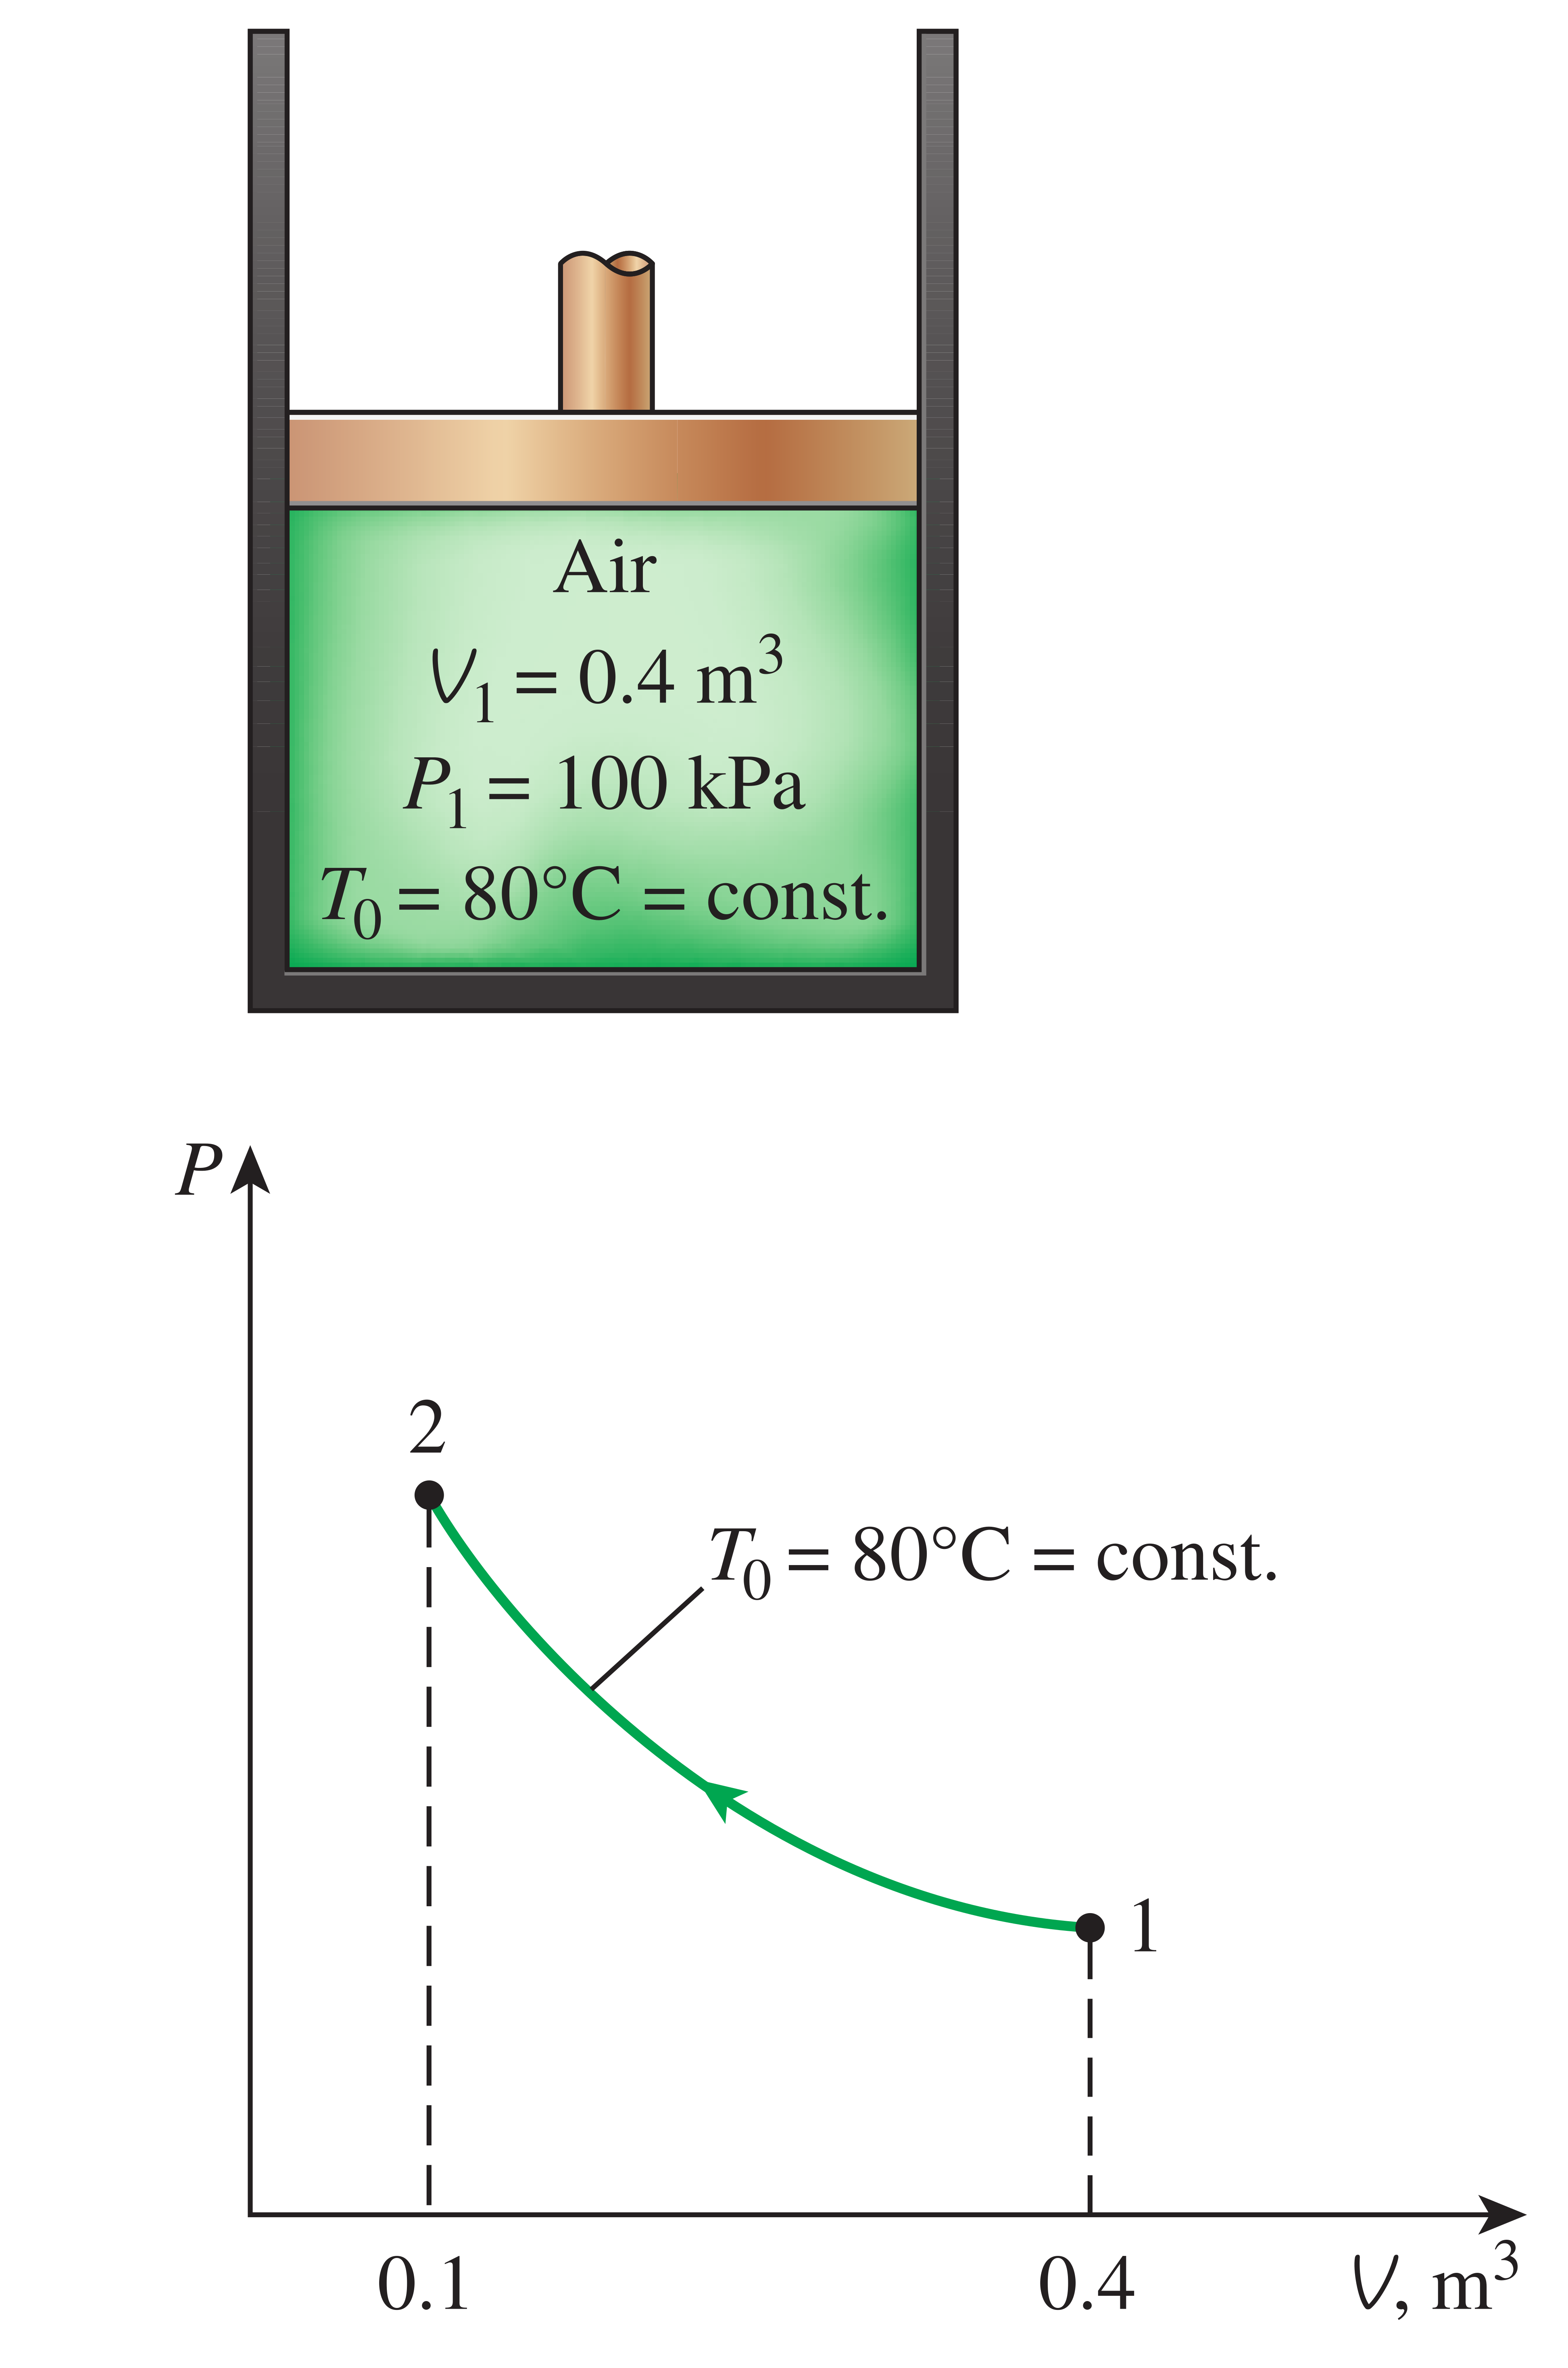
\includegraphics{isoT.png}
  \caption{Isothermal transformation \cite{2015}.}
  \label{fig:C3_isoT}
  \end{wrapfigure}
\quad\ The first type of transformations to be considered are the isothermal processes. Here, the transformation brings the system from states \textbf{1} to \textbf{2}, and the equality \(T_2 = T_1\)  is enforced. 

The transformation is said reversible isothermal if during all the processes the temperature remains constant. Such transformation is depicted in the Figure \ref{fig:C3_isoT}. The ideal gas equation (\ref{eq:C2_GP}) allows deriving the relation (\ref{eq:C3_isoT}) if the mass within the system does not vary.

\setstretch{1}
  \begin{align}
    p_1\cdot \mathrm{V}_1 &= p_2\cdot \mathrm{V}_2\nonumber\\
    \rightarrow p\cdot \mathrm{V} &= C \label{eq:C3_isoT}  
  \end{align}
  
\setstretch{1.5}
 For a compression or an expansion, the process is said isothermal if the system is respectively cooled or heat up to bring the final state temperature to the temperature of the initial state.
 
Considering an isothermal compression, the boundary work $W_b$, corresponding to the area below the curve, is given in the development (\ref{eq:C3_WbisoT}).

\begin{wrapfigure}{r}{0.3\linewidth}
  \centering
  \includegraphics{poly.png}
  \caption{Polytropic transformation \cite{2015}.}
  \label{fig:C3_poly}
\end{wrapfigure}
 \setstretch{1}
\begin{align}
  W_b &= \int_1^2 pd\mathrm{V} = C\cdot\int_1^2d\mathrm{V}\nonumber\\
  &= C\cdot \ln \frac{V_2}{V_1} = p_1\cdot V_1\cdot \ln \frac{V_2}{V_1} \label{eq:C3_WbisoT}
\end{align}

 \setstretch{1.5}
With $C$ being a constant coming from the integration. The value of this constant depends on the condition of inlet or outlet state.
\subsection{Polytropic transformation}
\quad\ The polytropic transformation, depicted in the Figure \ref{fig:C3_poly}, is  a generalization of the isothermal transformation. For an ideal gas, the polytropic transformation is characterized by the relation (\ref{eq:C3_poly}).

  \setstretch{1}
\begin{equation}
  p\cdot \mathrm{V}^n = C \label{eq:C3_poly}
\end{equation}

\setstretch{1.5}
Where $n$ is a constant. 
For $n=1$, the transformation simply corresponds to the isothermal transformation.\clearpage
 
\subsection{Isobaric transformation}
\begin{wrapfigure}{r}{0.3\linewidth}
  \centering
  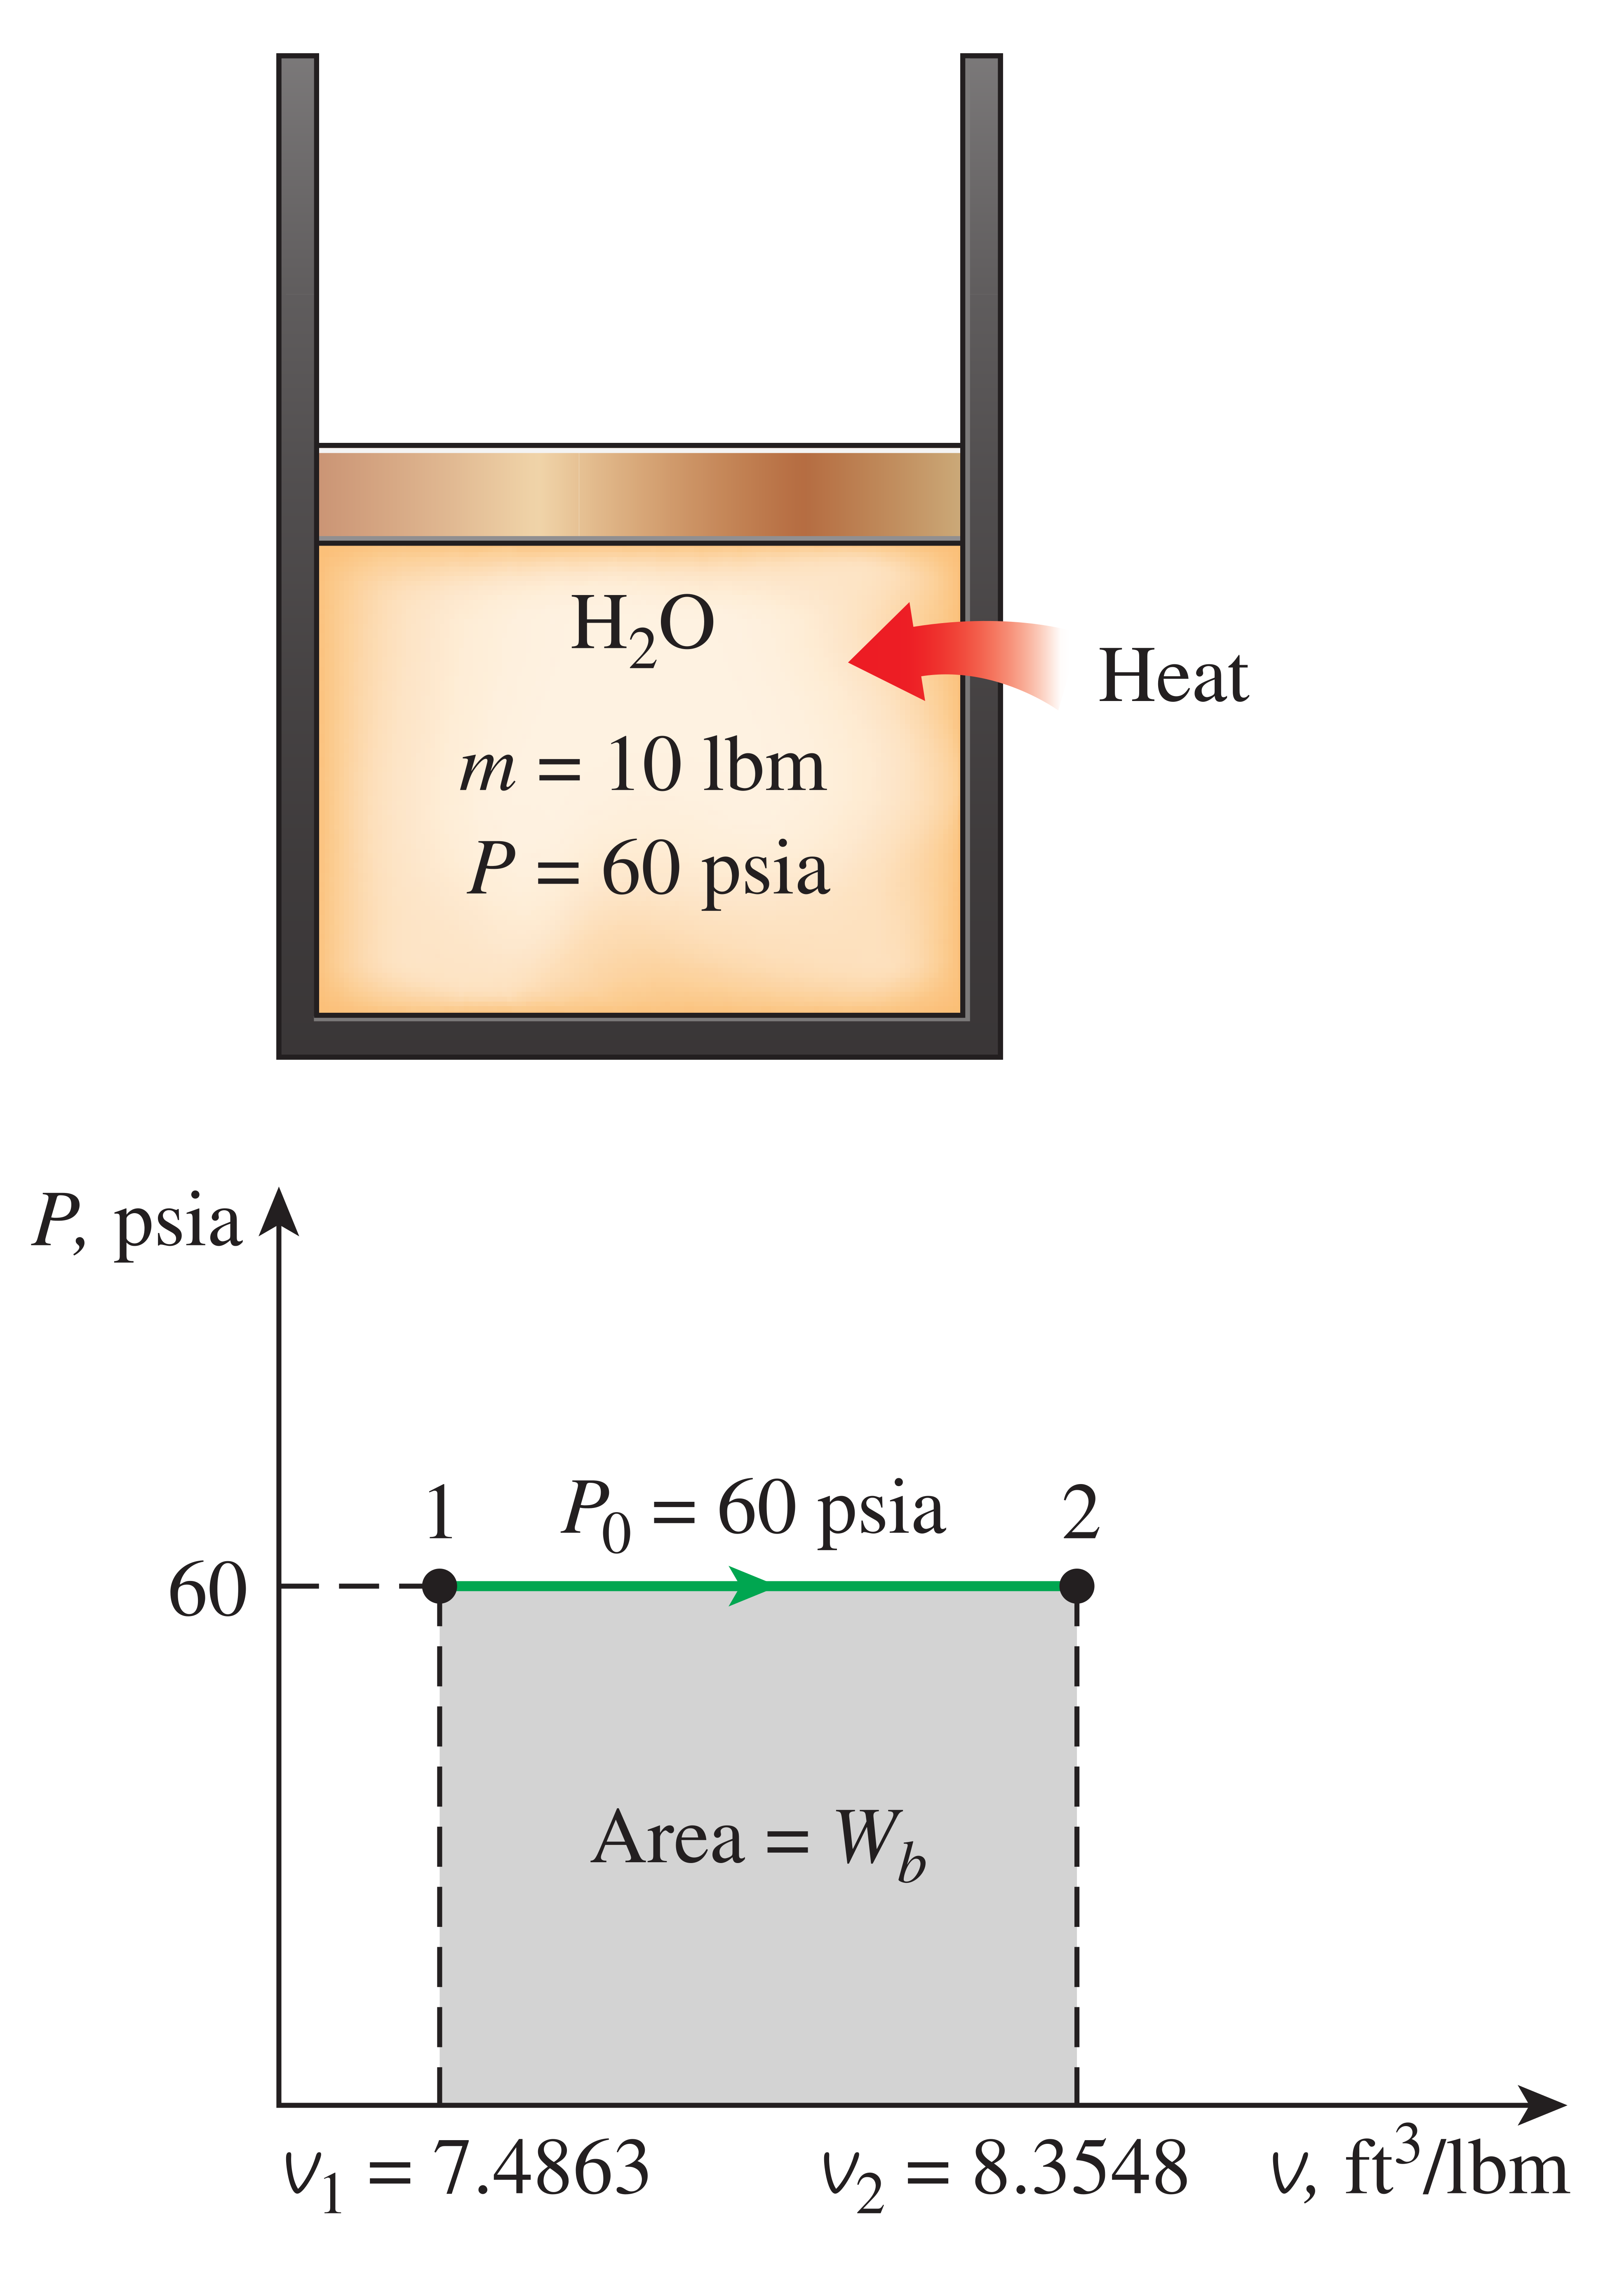
\includegraphics{isoP.png}
  \caption{Isobaric transformation \cite{2015}.}
  \label{fig:C3_isoB}
\end{wrapfigure}
\quad\ The isobaric transformation is one for which the initial and final state are both characterized by the same pressure. Thus, the equality \(p_2 = p_1 = p_0\) is enforced. 

The Figure \ref{fig:C3_isoB} illustrates such transformation. Typically, the transformation within the combustion chamber, heat exchanger or piping aim to be as close as this transformation. 

As for the isothermal transformation, the boundary work for an isobaric transformation is equal to the area below the curve. Here, the expression is given in the equation (\ref{eq:C3_WbisoP}).

  \setstretch{1}
\begin{align}
  W_b &= p_0\cdot \int_1^2d\mathrm{V}\nonumber\\
   &= p_0\cdot (\mathrm{V_2} - \mathrm{V_1}) = m\cdot p_0\cdot (\mathrm{v_2} - \mathrm{v_1}) \label{eq:C3_WbisoP}
\end{align}

\subsection{Isentropic transformation}
\setstretch{1.5}
\quad\ The last transformation to be considered is the isentropic transformation. This transformation corresponds to a reversible adiabatic transformation. 

Typically, when considering the expansion or the compression of a fluid, the manufacturers aim to build a machine which tends to minimize as much as possible the irreversibilities. 

\begin{figure}[h]
  \centering
  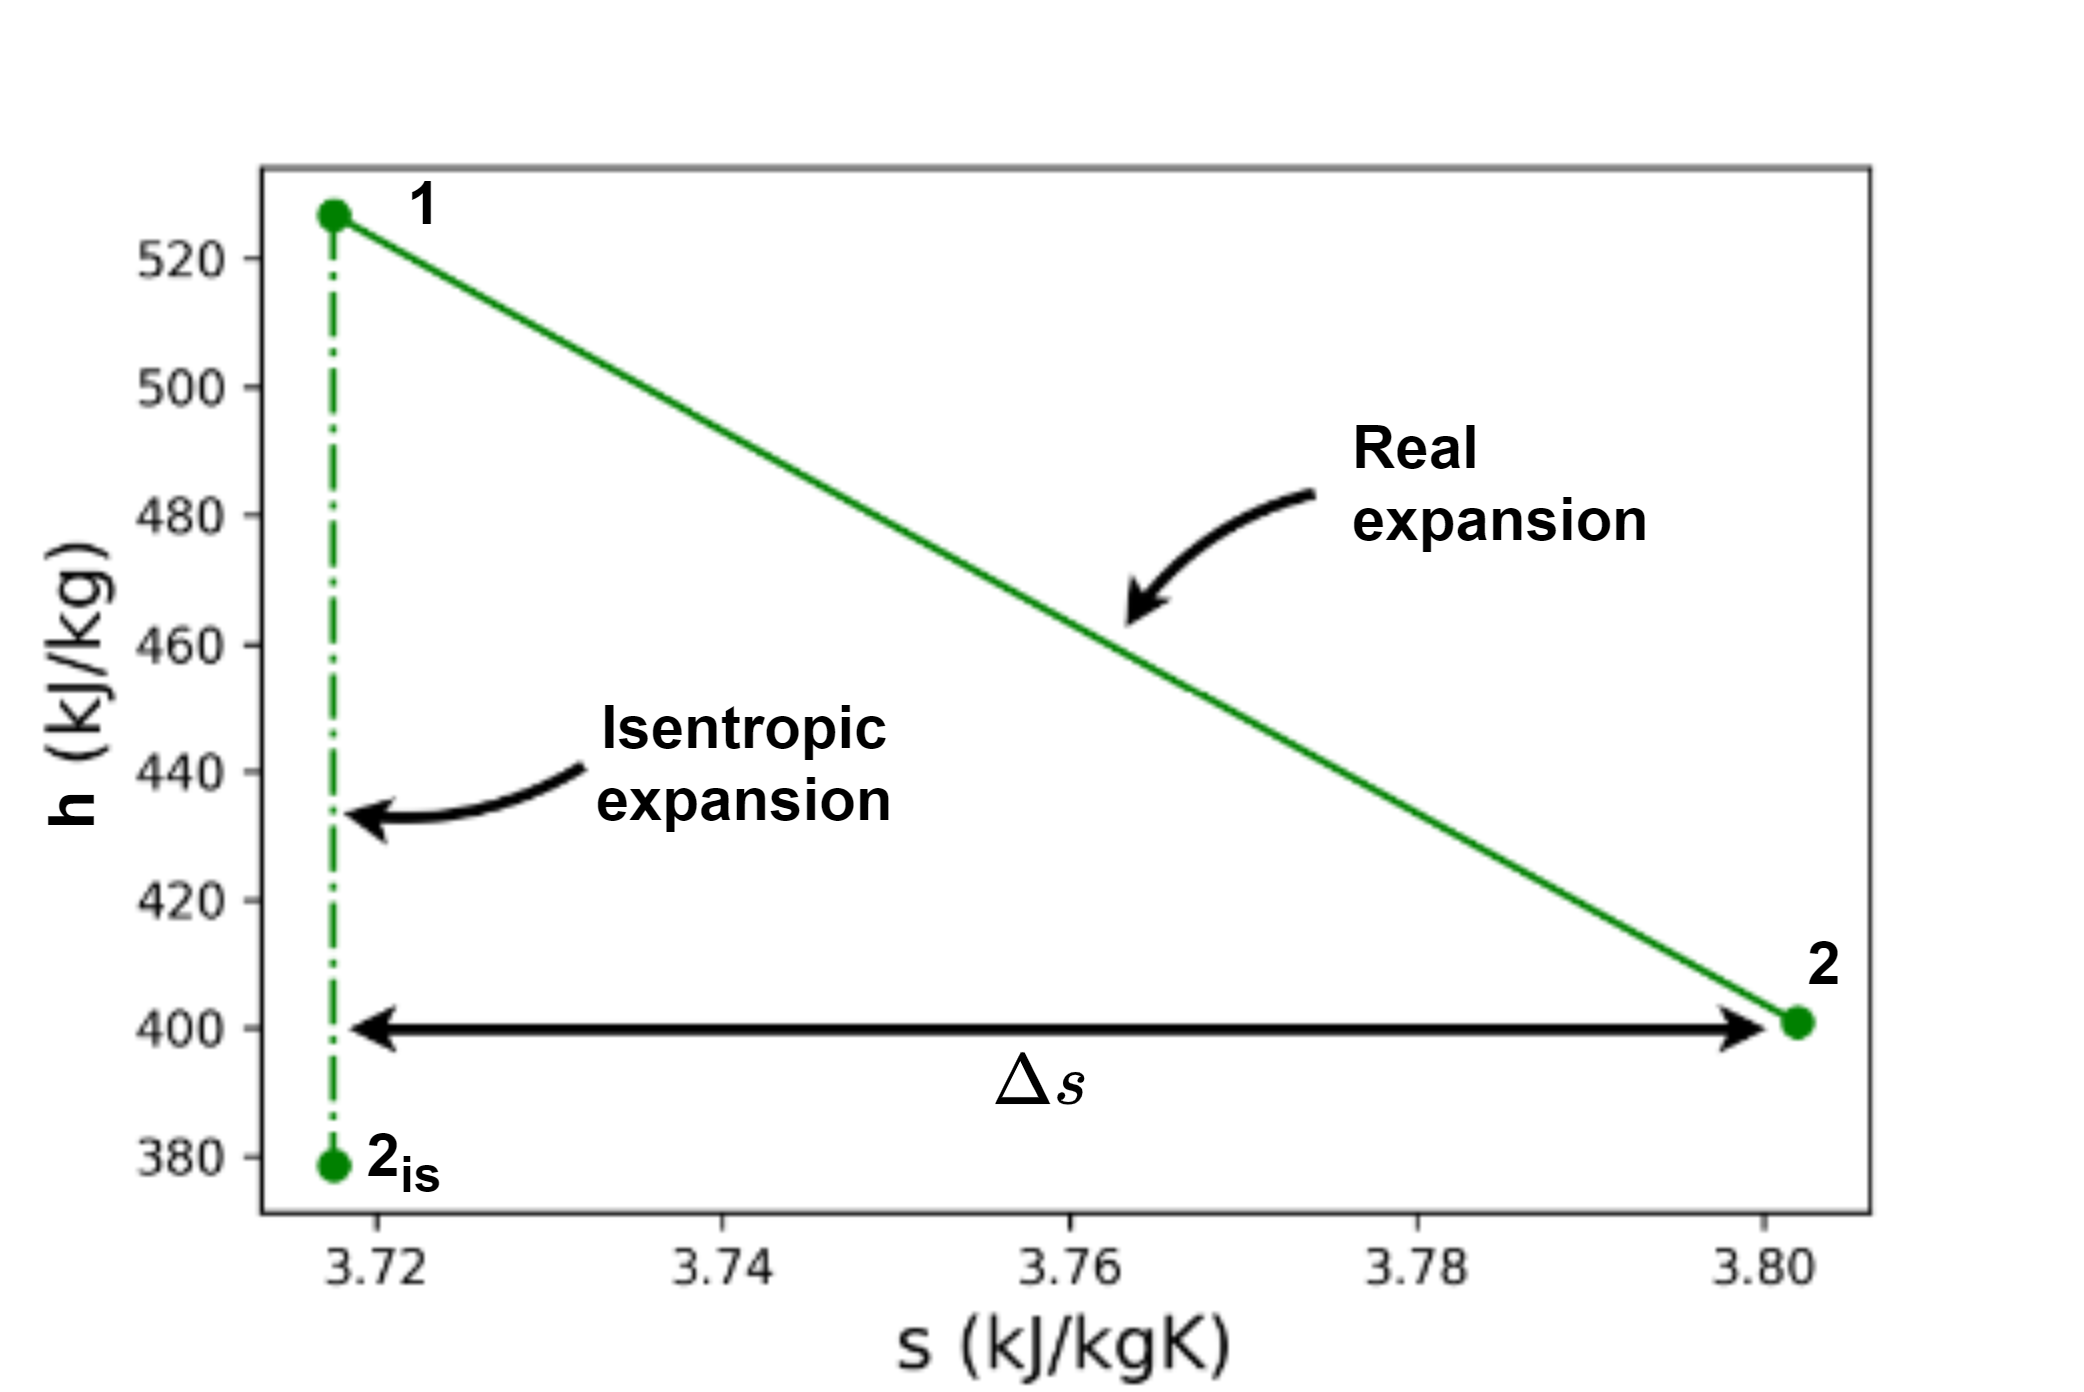
\includegraphics[width=0.6\textwidth]{expansion.png}
  \caption{Isentropic and real expansion.}
  \label{fig:C3_expansion}
\end{figure}
In the Figure \ref{fig:C3_expansion} is depicted an isentropic and a real expansion. As it can be noticed, the real expansion produces an augmentation of the entropy of the system. 

Moreover, the isentropic expansion is more efficient since the energy (in terms of enthalpy) extracted from the fluid is higher compared to the real expansion. The subscript "is" emphasizes the final state of the isentropic transformation.

It can be demonstrated that the enthalpy at the state \textbf{2$_{is}$} is always lower than the enthalpy at the state \textbf{2}. The consequence is that more work has been produced during the isentropic transformation. For an isentropic compression, the lower enthalpy $h_{2,is}$ implies that the work that the compression machine has to perform will be smaller.

\section{Thermodynamic properties}
\quad\, From now, the hypothesis of an ideal gas has been used for the computation of the previously established state variables. However, while this hypothesis remains quite valid when dealing with gas, it cannot be used for a real fluid (e.g. liquid water).

This problem can be solved using the Maxwell relations providing a linked between the partial derivatives of the different state variables $p$, $v$, $T$ and $s$ for a simple compressible system \cite{2015}. 

Those relations can be derived from the four Gibbs relations expressed in (\ref{eq:C3_Gibbs}).

\begin{subequations}
\setstretch{1}
\begin{equation}
  du = Tds - pdv \label{eq:C3_Gibbs1} 
\end{equation}    
\begin{equation}
  dh = Tds + vdp \label{eq:C3_Gibbs2} 
\end{equation}
\begin{equation}
  da = du - Tds - sdT = - pdv - sdT \label{eq:C3_Gibbs3} 
\end{equation}    
\begin{equation}
  dg = dh - Tds - sdT = vdp - sdT \label{eq:C3_Gibbs4}
\end{equation} \label{eq:C3_Gibbs}
\end{subequations}
where the state variables $a$ and $g$ are the Helmholtz and Gibbs function (respectively).
Analyzing these relations allows to notice that each of them are of the form

\begin{align}
\setstretch{1}
dz &= Mdx + Ndy\label{eq:C3_Maxbase}\\
\text{with } \left.\frac{\partial M}{\partial y}\right|_x &= \left.\frac{\partial N}{\partial x}\right|_y\label{eq:C3_partMax}
\end{align}
Using this property, the links between the different state variables are easily obtained by applying the relation (\ref{eq:C3_partMax}) to the equations (\ref{eq:C3_Gibbs1}) to (\ref{eq:C3_Gibbs4}).

\begin{subequations}
\setstretch{1}
\begin{equation}
  \left.\frac{\partial T}{\partial v}\right|_s =  - \left.\frac{\partial p}{\partial s}\right|_v \label{eq:C3_Max1} 
\end{equation}    
\begin{equation}
  \left.\frac{\partial T}{\partial p}\right|_s = \left.\frac{\partial v}{\partial s}\right|_p \label{eq:C3_Max2}  
\end{equation}
\begin{equation}
  \left.\frac{\partial s}{\partial v}\right|_T = \left.\frac{\partial p}{\partial T}\right|_v \label{eq:C3_Max3} 
\end{equation}    
\begin{equation}
  \left.\frac{\partial s}{\partial p}\right|_T =  - \left.\frac{\partial v}{\partial T}\right|_p \label{eq:C3_Max4} 
\end{equation} \label{eq:C3_Max}
\end{subequations}
The relations (\ref{eq:C3_Max}) are called Maxwell equations are helpful in thermodynamics. They provide a method to calculate the variation of the entropy of a system based on the measurement of the variation of the pressure, volume and temperature.

However, this method for calculating the thermodynamic variables is limited to simple compressible system and cannot be used when the system involves ''electrical, magnetic, and other effects''\cite{2015}.

These are the relations used when using a digital library for the thermodynamic assessment of the state of a pure fluid with real properties. The open-source library named \textbf{CoolProp}\cite{Bell2014} is one of the best known and. In this work, the library will be called many time when the ideal gas approximation is not relevant.
\section{Entropy variation}
\quad\, The previous section introduced the four equations of state (\ref{eq:C3_Gibbs1}) to (\ref{eq:C3_Gibbs4}). Among those, the second equation allows to write the relation (\ref{eq:C3_ds}).
\begin{equation}
ds = c_p\frac{dT}{T} - r\frac{dp}{p}\label{eq:C3_ds}
\end{equation}

By performing the integration over the path of a transformation going from state \textbf{1} to state \textbf{2}, the relation (\ref{eq:C3_s}) gives the link between the entropy variation and the temperature and pressure variation between the two states.

\begin{equation}
\setstretch{1}
s_2 - s_1  = \int_1^2\frac{c_p}{T}dT - r\cdot ln\frac{p_2}{p_1}\label{eq:C3_s}
\end{equation}
Supposing that the variation of the specific heat capacity with respect to temperature is negligible, the development (\ref{eq:C3_Deltas}) can be derived. 

\begin{equation}
\setstretch{1}
s_2 - s_1= r\cdot \left(\frac{k}{k-1}\cdot ln\frac{T_2}{p_1} - ln\frac{p_2}{p_1}\right) = r\cdot ln\left[\frac{p_1}{p_2}\cdot\left(\frac{T_2}{T_1}\right)^\frac{k}{k-1}\right] \label{eq:C3_Deltas}
\end{equation}
Where the $c_p=\frac{r\cdot k}{k-1}$ by using the two relations (\ref{eq:C3_r}) and (\ref{eq:C3_k}).

For an isentropic process, the equality $s_2=s_1$ is enforced. Thus, from (\ref{eq:C3_Deltas}) the relations (\ref{eq:C3_isrelPT}) and (\ref{eq:C3_isrelrhoT}) are obtained.

\begin{subequations}
\setstretch{1}
\begin{equation}
\frac{p_2}{p_1} = \left(\frac{T_2}{T_1}\right)^\frac{k}{k-1}\label{eq:C3_isrelPT}
\end{equation}
\begin{equation}
\frac{\rho_2}{\rho_1} = \left(\frac{T_2}{T_1}\right)^\frac{1}{k-1}
\label{eq:C3_isrelrhoT}
\end{equation}
\label{eq:C3_isrel}
\end{subequations}
\section{Isentropic efficiency} \label{C3:Isen_eff}
\quad\, For any real transformations, there is always an augmentation of the entropy when the system goes from its initial state \textbf{1} to its final state \textbf{2}. This implies that the difference $s_2 - s_1$ is greater than zero.

This can be characterized by defining the isentropic efficiency as being the image of the irreversibilities induced by the transformation. this type of efficiency is very frequently used when studying the compression or the expansion of a fluid.

For a compression or an expansion, the isentropic efficiency is defined by stating that the pressure ratio $\frac{p_1}{p_2}$ is the identical for both the isentropic and non isentropic transformation. Let's substituting this ratio by the constant $\Pi$. 

Considering first the ideal case, the equation (\ref{eq:C3_isrelPT}) gives after a reordering of the term the relation (\ref{eq:C3_Tis}).

\begin{equation}
\setstretch{1}
T_{2,is} = T_1\cdot\Pi^\frac{k-1}{k}\label{eq:C3_Tis}
\end{equation}

Then, for the real transformation, the left-hand-side of the relation (\ref{eq:C3_Deltas}) is greater than zero. This implies that the temperature at the end of the real transformation is always greater than the one at the en of the isentropic transformation. Thus, it leads to (\ref{eq:C3_T}).

\begin{equation}
\setstretch{1}
T_{2} > T_{2,is} = T_1\cdot\Pi^\frac{k-1}{k}\label{eq:C3_T}
\end{equation}
As can be noticed, the real transformation leads to a final state temperature bigger than for the isentropic transformation. This difference allows to define the isentropic efficiency $\eta_{is}$. The definition varies based on the desired transformation.
\begin{itemize}
\setstretch{1}
\item Compression: $\eta_{is}=\frac{T_{2,is}-T_1}{T_2-T_1}=\frac{h_{2,is}-h_1}{h_2-h_1}$
\item Expansion: $\eta_{is}=\frac{T_1-T_{2}}{T_1-T_{2,is}}=\frac{h_1-h_{2}}{h_1-h_{2,is}}$
\end{itemize}
Where the temperature and the enthalpy variation provide the same output result due to the ideal gas hypothesis. 

For a real fluid, the only valid definition of the isentropic efficiency is the one based on the enthalpy variation. 

\section{Exergy}
\quad\, The notion of energy has been introduced in the previous pages of this report. It has been seen that the energy can only be transformed. However, two with the same energy doesn't necessarily hold energy with the same quality. The quality of an energy is defined as being the potential that can be extracted from it. This can be quantified by the exergy, also called the available energy. \cite{2015} 

When performing an exergy analysis, the initial state of the system is specified, the transformation from the initial state to the final is done ''in a reversible manner, and the system is at a \textbf{dead state} at the end of the process.''\cite{2015}. A system at a dead state is a system that is in perfect equilibrium with its immediate surroundings. The Figure \ref{fig:C3_potato} depicts a system with its immediate surroundings circled in dashed red line.

\begin{figure}[h]
    \centering
    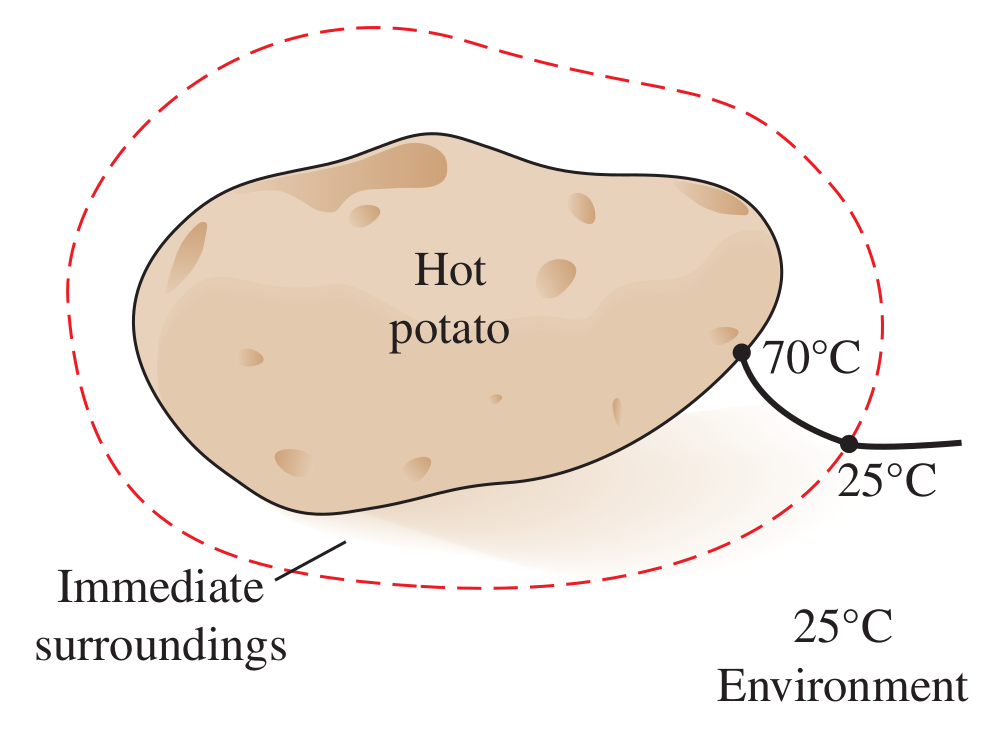
\includegraphics[width=0.45\textwidth]{Chapitre_3/Images/potato.png}
    \caption{Hot Potato \cite{2015}.}
    \label{fig:C3_potato}
\end{figure}

When a system is at a dead state, it cannot deliver any extra energy to its (immediate) surrounding. This means that the work done by the system has been maximized. If a gradient of temperature remains between the system and the immediate surroundings, extra could be produced by ''running a heat engine these two levels of temperature.''\cite{2015} 

This represents the useful work potential of the system and is called exergy. ''The exergy provides an  upper limit on the amount of work a device can deliver without violating any thermodynamic laws.''\cite{2015}


\newpage
%%%%%%%%%%%%%%%%%%%%%%%%%%%%%%%%%
%% Chapitre 4:                 %%
%% Thermodynamics components   %%
%%%%%%%%%%%%%%%%%%%%%%%%%%%%%%%%%
\graphicspath{{Chapitre_4/Images/}}
\chapter{Thermodynamic components}\label{C4}
%%%%%%%%%%%%%%%%%%%%%%%%%%%%%%%%%%%
%%%%%                         %%%%%
%%%%% Introduction chapitre 3 %%%%%
%%%%%                         %%%%%
%%%%%%%%%%%%%%%%%%%%%%%%%%%%%%%%%%%
\quad\ In the beginning of the previous chapter, it has been mentioned that the Brayton cycle composed of several components that are more or less complex. The behavior of these components, which is required to realize the study of the global system, is based on the thermodynamic notions that have been introduced all along the past lines.

This chapter will be focused on the description of those components. For each of them, it will be provided the concepts or principles that will be used during this work. Then, a description of the Brayton cycle itself will be provided. Different configurations will be proposed and compared.
\section{Turbomachines}
%%%%%%%%%%%%%%%%%%%%%%%%%%%%%%%%%%%
%%%%%                         %%%%%
%%%%%    <<Turbomachines>>    %%%%%
%%%%%                         %%%%%
%%%%%%%%%%%%%%%%%%%%%%%%%%%%%%%%%%%
\quad\ The first family of components to be studied is the turbomachines. The machines included this family are ones ''that exchange energy between the
fluid traversing it and mechanical energy supplied to or extracted from the machine''\cite{Hillewaert2019}. Those machines are \textbf{rotating} machines that
can be categorized into two families.

The first family of turbomachines is ones which inject or extract energy from an incompressible flow. These transformations on the fluid  are respectively performed by the pumps and hydraulic turbines.

The second family is turbomachines dealing with compressible flow. Here, some extra effects are taken into account. For instance, the velocity of the flow can be at some points limited due to choking effects. Also, since the flow is compressible its density can vary along the path, the velocity will vary along the path as well. 

Turbomachines that are encompassed in this second category are compressors and gas turbines. As for the pumps and hydraulic turbines, compressors and turbines aim to inject and extract energy into/from the flow.

\subsection{General principles}
\quad\ Some principles used when designing incompressible and compressible flow based machines are common for both of these families. Among these principles, it can be emphasized the velocity triangle, the enthalpy and rhotalpy conservation principles, and the similarity analysis. 

The velocity triangle and the conservation principles provide tools to well design the blades of the turbomachines.  The similarity is used to derive the performance of a given machine based on non-dimensional quantities. The following lines will explain the basis of these different principles. 

\subsubsection{Velocity triangle}
\quad\ When considering the rotating part of the turbomachine (named rotor), there is, in addition to the absolute frame of reference, a rotating frame which is attached to the rotor. This leads to definition of three components for the velocity of the fluid: 

\begin{itemize}
\setstretch{1}
    \item Absolute velocity \(\mathbf{v}\): Velocity of the fluid in the absolute frame (\(\mathbf{x},\mathbf{y}\)).
    \item Tip blade velocity of the rotor \(\mathbf{u_r}\): Velocity of the tip of the rotor blades in the absolute frame (\(\mathbf{x},\mathbf{y}\)).
    \item Relative velocity \(\mathbf{w_r}\): Velocity of the fluid in the relative frame  (\(\mathbf{x'},\mathbf{y'}\)).
\end{itemize}

\begin{figure}[h]
    \centering
    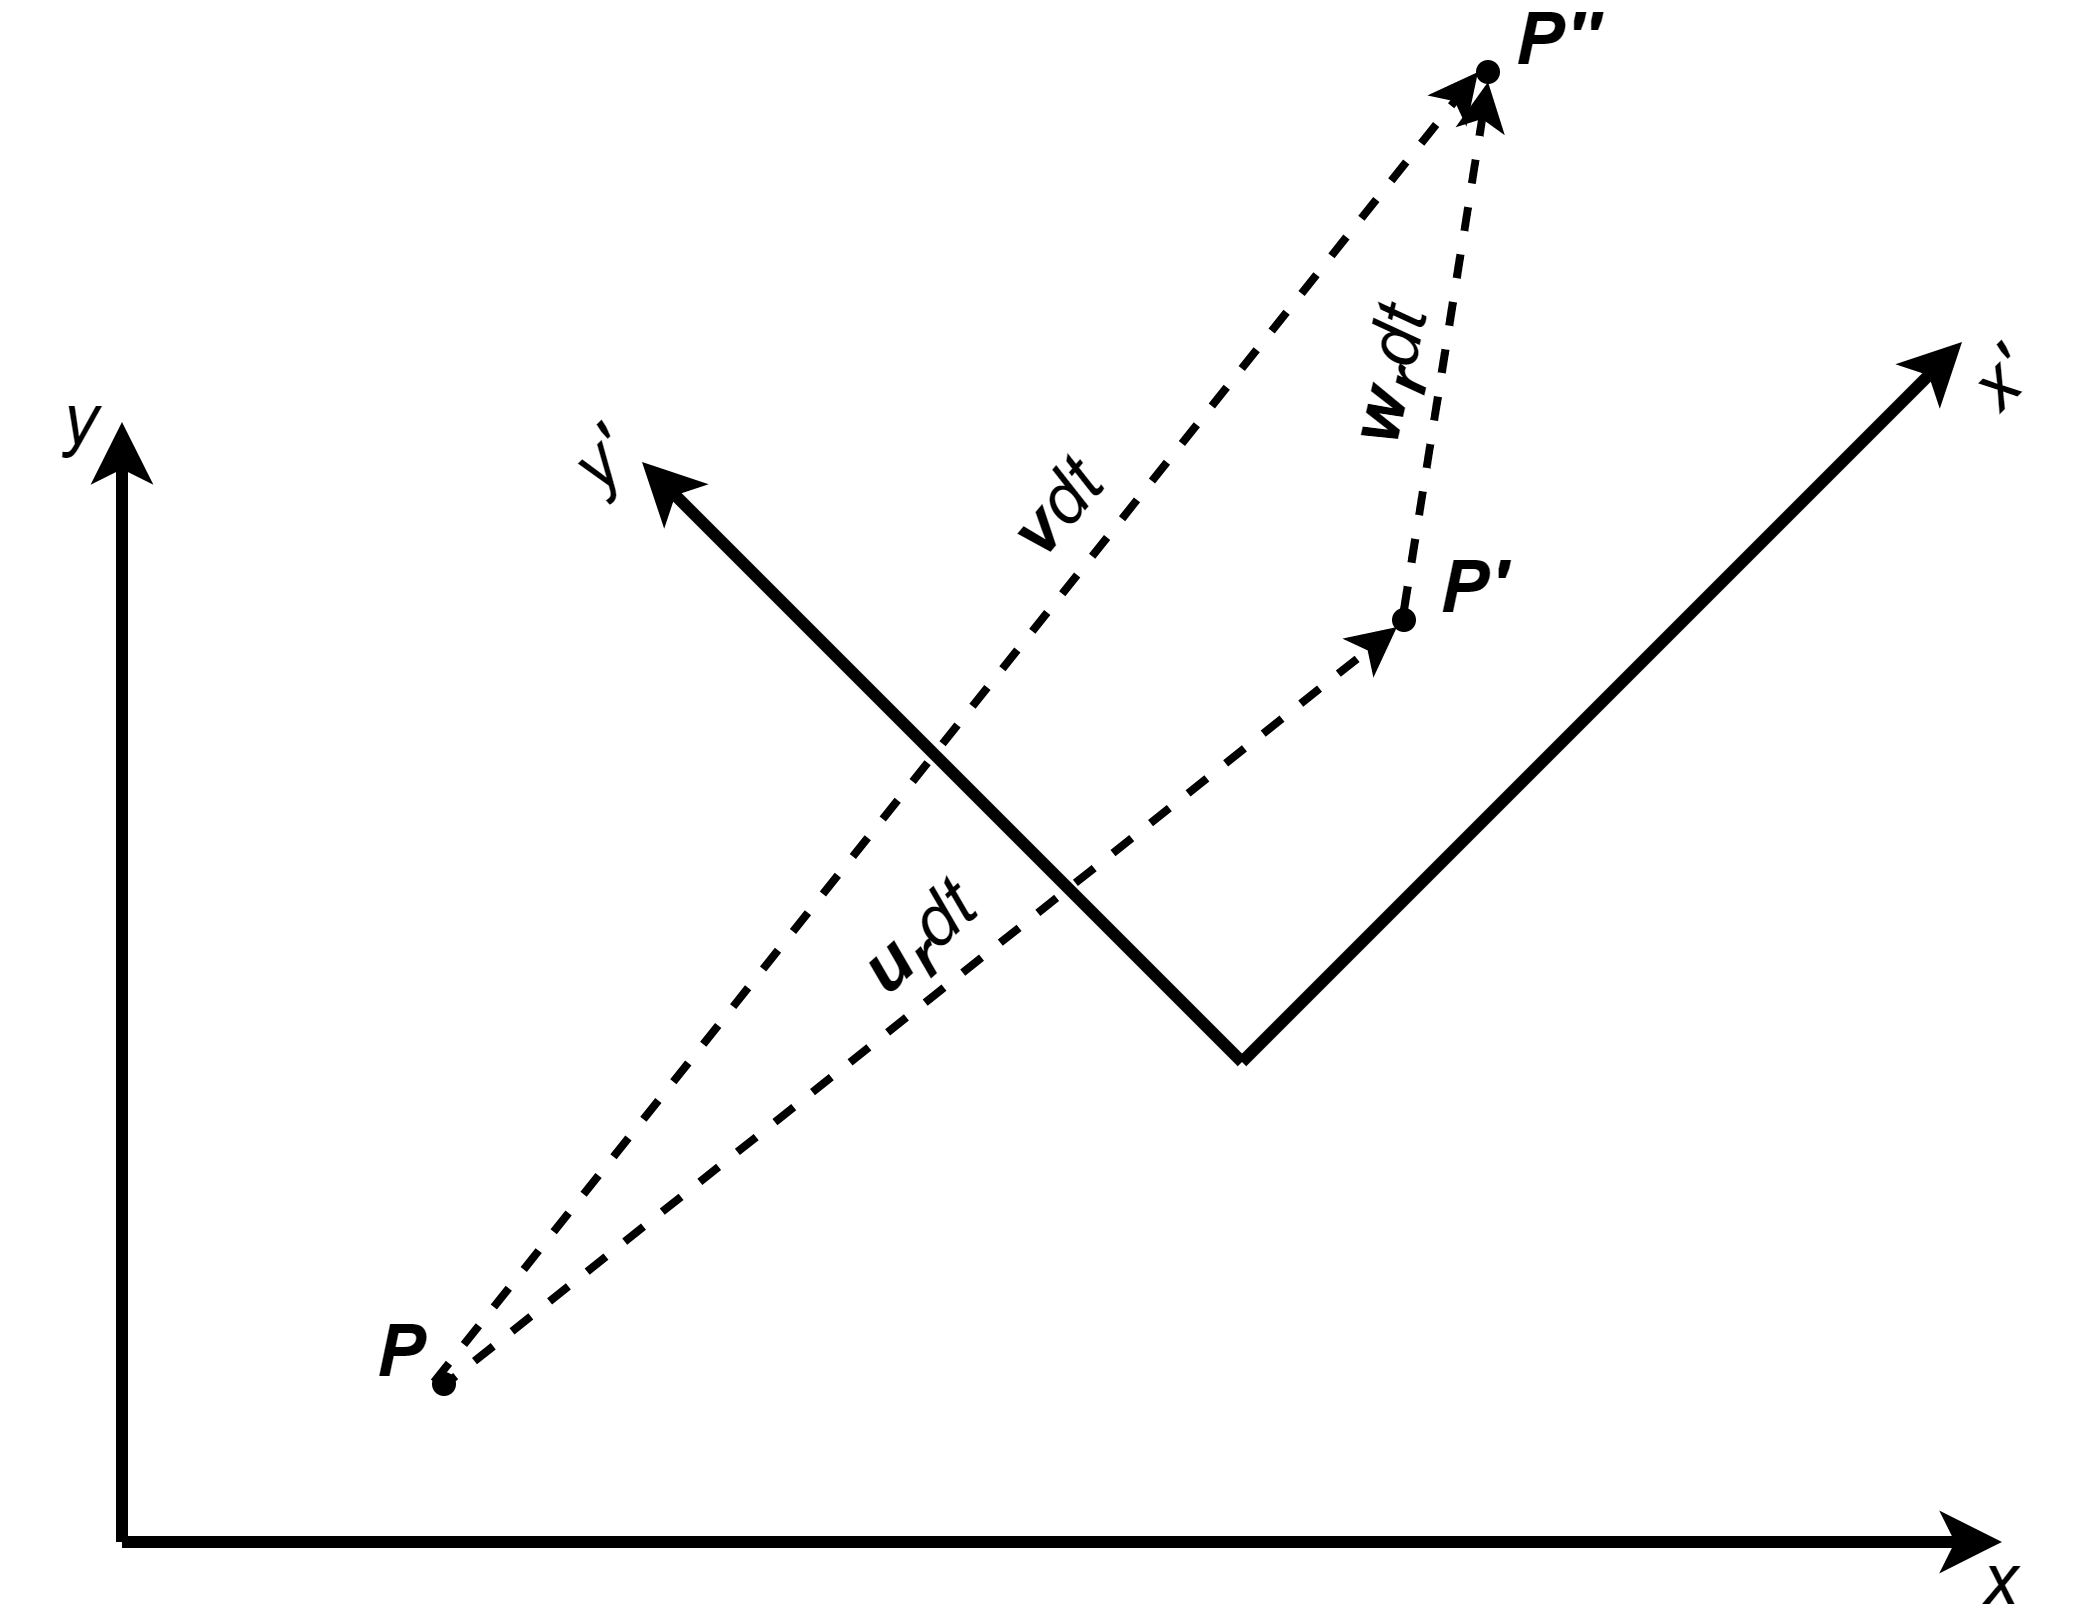
\includegraphics[width=0.6\textwidth]{Frames.png}
    \caption{Absolute and rotating frames.}
    \label{fig:C4_frames}
\end{figure}

The Figure \ref{fig:C4_frames} shows the representations in the space of these different definitions of the velocity. Considering a point at $P$ at the time t=0, this point is moving to \(P''\) at the time t=dt.  
The drawing shows that the following vectorial equality (\ref{eq:C4_velocity}) is enforced at any time.

\begin{equation}
    \setstretch{1}
    \mathbf{v} = \mathbf{u_r} + \mathbf{w_r} \label{eq:C4_velocity}
\end{equation}

Another way of representations of these velocities is to draw the velocity triangle. The velocity triangle is defined as depicted in the Figure \ref{fig:C4_vtriang}.

\begin{figure}[h]
    \centering
    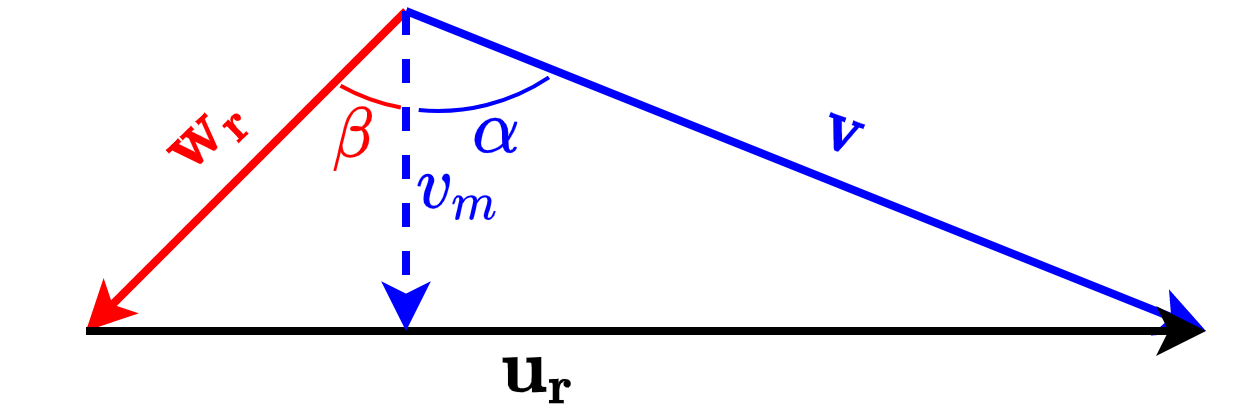
\includegraphics[width=0.6\textwidth]{Vtriangle.png}
    \caption{Velocity triangle.}
    \label{fig:C4_vtriang}
\end{figure}
Where $v_m$ is the projection of the vector $\mathbf{v}$ on the meridional axis.

Here, two angles $\alpha$ and $\beta$, respectively the absolute and relative flow angles, can be defined. Those angles will allow designing the shape of the rotating blade based on the desired applications. 

\subsubsection{Enthalpy and rothalpy conservation}
\quad\ It has been mentioned before that, for a compressible flow, the velocity can vary along the path. The notion of static and total (or stagnation) quantities have been established to take into account this variation of velocity. Stagnation quantities will be identified by the superscript ''0''.

For instance, the total enthalpy is given by
\begin{equation}
    \setstretch{1}
    h^0 = h + \frac{1}{2}\cdot v^2\label{eq:C4_h0}
\end{equation}

Now, considering an adiabatic transformation without viscous work, the total enthalpy is conserved between the initial state and the final state.
\begin{equation}
    \dot{m}_1\cdot h_1^0 = \dot{m}_2\cdot  h_2^0 \label{eq:C4_hcons}
\end{equation}
Which can be reduced to \(h_1^0 = h_2^0\) if we supposed that the transformation is performed without any leakages (\(\dot{m}_1=\dot{m}_2\)). The states \(1\) and \(2\) are associated to the orthogonal boundaries to the flow of the selected control volume delimiting the studied system.

\begin{equation}
    \setstretch{1}
    i^0 = h + \frac{1}{2}\cdot w_r^2 - \frac{1}{2}\cdot u_r^2 \label{eq:C4_i0}
\end{equation}

Similarly, using the definition (\ref{eq:C4_i0}) of the stagnation rhotalpy, it is obtained from the Euler equation (\ref{eq:C4_Euler}) that, within a rotor, the total rothalpy is conserved through the transformation process.

\begin{align}
    \setstretch{1}
    h_2^0 - h_1^0 = \frac{1}{2}\cdot & \left(v_2^2 - v_1^2\right) - \frac{1}{2}\cdot \left(w_{r,2}^2 - wr_{r,1}^2\right) + \frac{1}{2}\cdot \left(u_{r,2}^2 - u_{r,1}^2\right)\label{eq:C4_Euler} \\
    \text{with }                     & v = \left|\vect{v}\right|\quad\text{;}\quad  w_r = \left|\vect{w_r}\right|\quad\text{;}\quad u_r= \left|\vect{u_r}\right|\nonumber
\end{align}

The rhotalpy conservation is then expressed as stated in the equality (\ref{eq:C4_icons}).

\begin{equation}
    \setstretch{1}
    \dot{m}_1\cdot i_1^0 = \dot{m}_2\cdot i_2^0 \label{eq:C4_icons}
\end{equation} 

\subsubsection{Similarity}
\quad\ The design of the turbomachines often requires validations through experimental testing.  

However, because the design of the turbomachines really depends on the application in view, creating a new test bench for each machine is time consuming and has a high cost. 

Thus, the analysis by similarity has been established to 
minimize the number of experimental campaign that has to be conducted. By defining some non-dimensional quantities describing the operating point of a given turbomachine, it is possible to extrapolate similar operating points of the same machine or, operating point of a similar machine of another size. 

This is a really powerful tool which allows to significantly decrease the time and the cost related to the design of a new turbomachine. Indeed, it allows to do the testing on smaller turbomachines, and then the performance of the desired machine are extrapolated. Since the machines and the associated test benches are smaller, the cost of the experimental campaign is significantly smaller, and the experimental results can be reused for future designed machines.
\subsection{Pumps and hydraulic turbines}
\quad\, Now that the base principles have been introduced, those can be utilized to perform an analysis of turbomachines with incompressible flow. 

Among the machine exchanging energy with such type of fluid, it can be distinguished the pumps, which are designed to raise the height (or total hydraulic energy) \(h\) of the fluid, and the hydraulic turbines which do the opposite transformation. 

The variation of the height of the fluid is similar to its enthalpy variation. Thus, the respective power consumed and produced \(\dot{W}_p\) by  the pump and the hydraulic turbine can be expressed as given in the relation (\ref{eq:C4_Pinc}), noting that the transformation makes the system going from state \textbf{a} to state \textbf{b}.
\begin{equation}
    \dot{W}_{p,a-b} = \dot{m}\cdot (h_a - h_b)=\dot{m}\cdot\Delta h_p \label{eq:C4_Pinc}
\end{equation}


If the consumed power of the pump is \(\dot{W}_{e,a-b}\), its global efficiency \(\eta_p\) is equal to the ratio
\begin{equation}
    \eta_p = \frac{\dot{W}_{p,a-b}}{\dot{W}_{e,a-b}}\label{eq:C4_Etapump}
\end{equation}
\subsubsection{Characteristic maps}
\quad\ It has been shown that the power output and the global efficiency of the pump are functions of the height variation and the flow rate of the fluid. When operating a pump, it can be useful to know how this height variation will vary with respect to the flow rate and the rotational speed of the pump shaft. The knowledge of these two parameters allows to fully characterized the pump.

Considering the volumetric flow rate \(\dot{\mathrm{V}}\) (m$^3$/s) and the rotational speed \(N\), the two following relations (\ref{eq:C4_DHp}) and (\ref{eq:C4_Pe}) can be derived.

\begin{subequations}
    \setstretch{1}
    \begin{equation}
        \Delta h_p(\dot{\mathrm{V}}_p, N_p)\label{eq:C4_DHp}\\
    \end{equation}
    \begin{equation}
        \dot{W}_{elec}(\dot{\mathrm{V}}_p, N_p)\label{eq:C4_Pe}
    \end{equation}
\end{subequations}
Those relations will be called characteristic or performance map and has to be determined \textbf{experimentally}. An example of such map is given in the Figure \ref{fig:C4_MapPump}.
\begin{figure}[h]
    \centering
    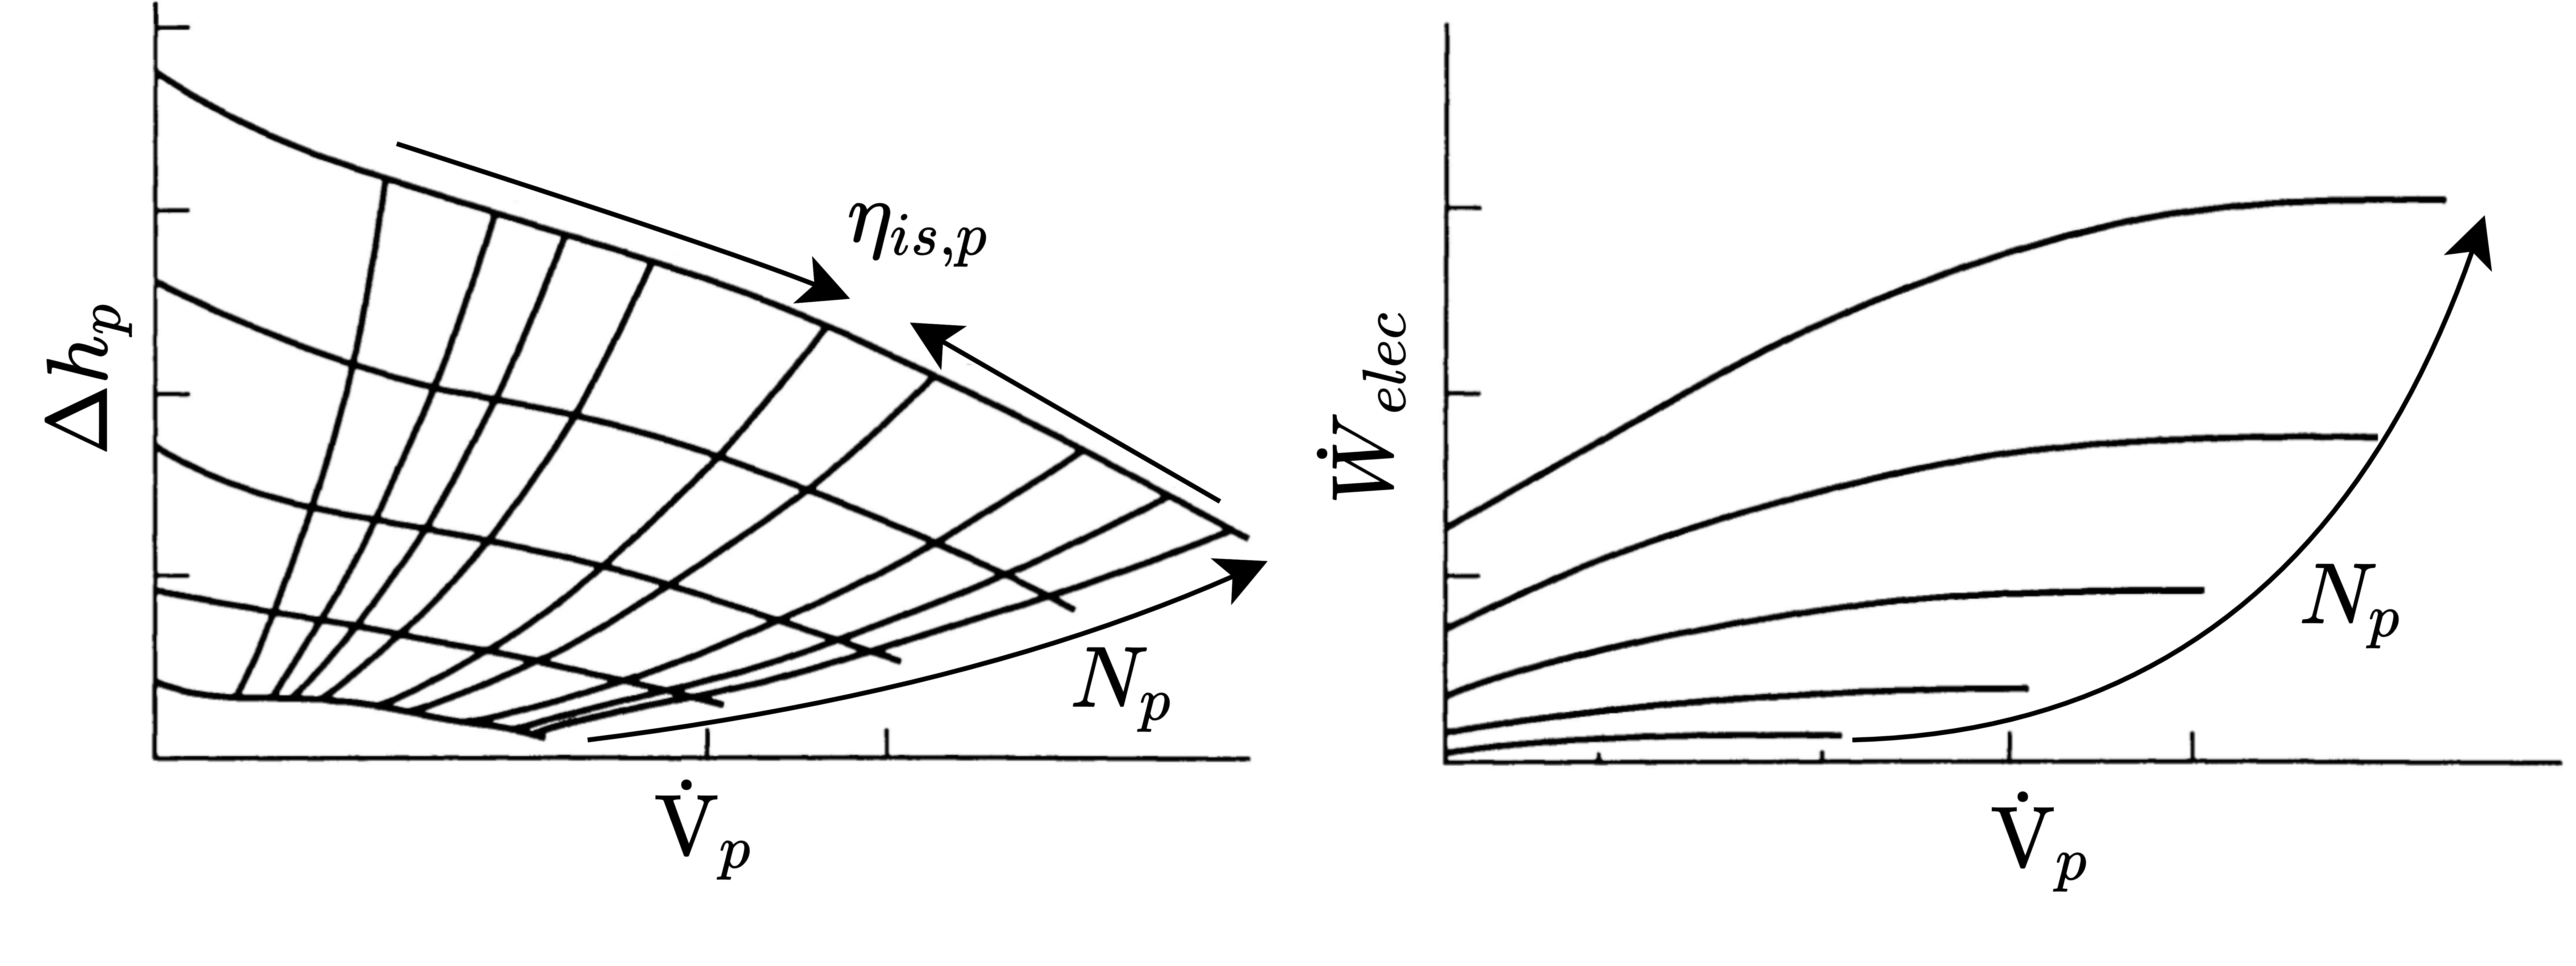
\includegraphics[width=0.8\textwidth]{Pump_map.png}
    \caption{Characteristic maps of a pump \cite{Hillewaert2019}.}
    \label{fig:C4_MapPump}
\end{figure}

However, not all the operating points constituting the performance map has to be computed through an experimental campaign. Indeed, using the similarity analysis described during the previous section, determining the operating points for one rotational speed is sufficient to deduce the rest of the characteristic map.

\begin{subequations}
    \begin{equation}
        \phi = \frac{\dot{\mathrm{V}_p}}{N_p\cdot r_2^3}\label{eq:C4_phipump}
    \end{equation}
    \begin{equation}
        \psi = \frac{4\cdot g\cdot \Delta h_p}{N_p^2\cdot r_2^2}\label{eq:C4_psipump}
    \end{equation}
\end{subequations}

For the pump, the non-dimensional head and flow coefficients \(\phi\) and \(\psi\) are defined based on the outlet condition \textbf{2} of the pump. Those coefficients are respectively defined by the relations (\ref{eq:C4_phipump}) and (\ref{eq:C4_psipump}), \(r_2\) being the outlet radius of the pump. 

From the definitions of these two non-dimensional quantities, the height variation \(\Delta h_p\) and the volumetric flow rate $\dot{\mathrm{V}}$ can be obtained for any rotational speed. 

Considering that the operating point (\(\dot{\mathrm{V}}_1, \Delta h_{p,1},N_1\)) is known, the similar operating point\linebreak (\(\dot{\mathrm{V}}_2, \Delta h_{p,2},N_2\)) for any rotational speed \(N_2\) can be obtained using the relations (\ref{eq:C4_Qsim}) and (\ref{eq:C4_DHsim}).

\begin{subequations}
    \setstretch{1}
    \begin{equation}
        \dot{\mathrm{V}}_{p,2} = \dot{\mathrm{V}}_{p,1}\cdot\frac{N_{p,2}}{N_{p,1}} \label{eq:C4_Qsim}
    \end{equation}
    \begin{equation}
        \Delta h_{p,2} = \Delta h_{p,1}\cdot\left(\frac{N_{p,2}}{N_{p,1}}\right)^2 \label{eq:C4_DHsim}
    \end{equation}\label{eq:C4_sim}
\end{subequations}

These relations stand since for any similar point of operation, the non-dimensional quantities remain constant. Consequently, the pump isentropic efficiency remains constant as well.

Similar reasoning can be performed for the hydraulic turbines. For hydraulic turbines, the head and flow coefficients are defined based on the inlet condition \textbf{1} of the turbines.

\subsection{Compressible flow}
\quad\ The previous subsection introduced the pump which is a turbomachine design to increase the energy of the incompressible fluid passing through it. However, this type of machine cannot deal with compressible flow for which the density can vary over the distance. For instance, the air is a compressible fluid.

The behavior of the compressible flow is more complex to describe compared to incompressible flow. Indeed, “compressible flow is characterized by the propagation of acoustic waves” \cite{Hillewaert2019}.   This part of the section about turbomachines will only focus on the main principles required for the good understanding of this work.


\subsubsection{Velocity triangle}
\quad\ With the relation (\ref{eq:C4_Euler}), the notion of absolute and relative velocity of the flow has been introduced. A graphic representation of these three vectors can be done using the \textbf{velocity triangle}. This triangle is drawn in the Figure \ref{fig:C4_vtriang}.

\subsubsection{Mach number}
The Mach number \(M\) is defined as being the ratio between the velocity \(v\) and the sound speed \(c\).
\begin{equation}
    M = \frac{v}{c} \label{eq:C4_Mach}
\end{equation}
The Mach number \(M\) is a dimensionless variable that gives an image of the compressible effects of the flow. Thus, one criterion for the determination of similar operational points is to keep the Mach number constant.

Using the Mach number allows obtaining formulas to compute the total quantities based on the static ones. By considering first the total temperature, the relation (\ref{eq:C4_TT0_1}) can be found.
\begin{equation}
    T^0 = T + \frac{v^2}{2\cdot c_p} = T\cdot\left(1 + \frac{v^2}{2\cdot c_p\cdot T}\right)\label{eq:C4_TT0_1}
\end{equation}
For an isentropic process, it can be demonstrated that the speed of sound \(a=k\cdot r\cdot T\). Thus, the equation (\ref{eq:C4_TT0_1}) becomes (\ref{eq:C4_TT0}).
\begin{equation}
    T^0 = T\cdot\left(1 + \frac{k-1}{2}\cdot M^2\right) = T\cdot f_M(M) \label{eq:C4_TT0}
\end{equation}
Using the equations (\ref{eq:C3_isrelPT}), (\ref{eq:C3_isrelrhoT}) from chapter \ref{C3} and the definition of the function \(f_M(M)\), the relations linking the static to the total pressure, density and speed of sound can be obtained as well.

\begin{subequations}
    \setstretch{1}
    \begin{equation}
        p^0 = p\cdot f_M(M)^\frac{k}{k-1}\label{eq:C4_PP0}
    \end{equation}
    \begin{equation}
        \rho^0 = \rho\cdot f_M(M)^\frac{1}{k-1}\label{eq:C4_rhorho0}
    \end{equation}
    \begin{equation}
        c^0 = c\cdot\sqrt{f_M(M)} \label{eq:C4_aa0}
    \end{equation}
\end{subequations}\newpage

\subsubsection{Characteristic maps}
\quad\ As for the turbomachines exchanging energy with incompressible flow, those dealing with compressible flow can also be fully characterized knowing a pair of independent operating parameters. The most usual parameters are

\begin{itemize}
    \setstretch{1}
    \item \(\dot{m}_{corr}\) (kg/s): It is the corrected mass flow rate.
    \item \(\Pi_{tt}\) (-): It is the total to total pressure ratio across the turbomachine. It is always defined to be greater than one.
    \item \(N_{corr}\) (RPM): It is the corrected rotational speed of the turbomachine. 
    \item \(\eta_{is}\) (-): It is the total to total isentropic efficiency of the turbomachine.
\end{itemize}
It can be demonstrated that the performance map of a turbomachine is determined by relations between 3 non-dimensional groups.

Considering an operating point $a$ characterized by the mass flow rate $\dot{m}_a$, the rotational speed $N_a$, and the inlet stagnation temperature and pressure $T^0_{1,a}$ and $p^0_{1,a}$, it is possible to derive any similar operating points. By applying the formula (\ref{eq:C4_mab}) and (\ref{eq:C4_Nab}), the mass flow rate $\dot{m}_b$ and rotational speed $N_b$ at the similar operating point $b$ characterized by the stagnation inlet state ($T^0_{1,b}$, $p^0_{1,b}$) can be computed.

\begin{subequations}
\setstretch{1}
\begin{align}
    \dot{m}_{b} &= \dot{m}_{a}\cdot\sqrt{\frac{T^0_{1,a}}{T^0_{1,b}}}\cdot\frac{p^0_{1,b}}{p^0_{1,a}}\label{eq:C4_mab}\\
    N_b &= N_a\cdot \sqrt{\frac{T^0_{1,b}}{T^0_{1,a}}}\label{eq:C4_Nab}
\end{align}    
\end{subequations}

These two relations allow going from one operating point to the other without modifying the value of the non-dimensional quantities. Therefore, going from $a$ to $b$ will not modify the pressure ratio $\Pi_{tt}$, the isentropic efficiency $\eta_{is}$ and the Mach number $M$.

In particular, if the operating point $b$ considered is defined at the reference conditions ($T_{ref},P_{ref}$), the associated mass flow rate and rotational speed are called \textbf{corrected} mass flow rate $\dot{m}_{corr}$ and \textbf{corrected} rotational speed $N_{corr}$. Thus, from a measured operating point, these two corrected quantities are obtained by applying the relation (\ref{eq:C4_mc}) and (\ref{eq:C4_Nc}).

\begin{subequations}
\setstretch{1}
\begin{align}
    \dot{m}_{corr} &= \dot{m}\cdot \frac{\sqrt{\theta_T}}{\theta_p}\label{eq:C4_mc}\\
    N_{corr} &= \frac{N}{\sqrt{\theta_T}}\label{eq:C4_Nc}
\end{align}    
\end{subequations}
Where $\theta_T = \frac{T^0}{T_{ref}}$ and $\theta_p = \frac{p^0}{p_{ref}}$. $T^0$ and $p^0$ are respectively the stagnation temperature and pressure observed at the inlet of the turbomachine.

Alternatively, the reduced mass flow rate \(\dot{m}_{r}\) can also be used to assess the performance of the turbomachines. This non-dimensional quantity is as follows:

\begin{equation}
    \setstretch{1}
    \dot{m}_r = \dot{m}\cdot \frac{\sqrt{T^0}}{p^0}
\end{equation}

Now, if the rotational speed $N$ and the mass flow rate $\dot{m}$ are assumed to be known, the two other quantities $\Pi_{tt}$ and $\eta_{is}$ can be calculated using the relations (\ref{eq:C4_Pimap}) and (\ref{eq:C4_etamap}).

\begin{subequations}
    \setstretch{1}
    \begin{equation}
        \Pi_{tt}(N_{corr}, \dot{m}_{corr})\label{eq:C4_Pimap}
    \end{equation}
    \begin{equation}
        \eta_{is}(N_{corr}, \dot{m}_{corr})\label{eq:C4_etamap}
    \end{equation}
\end{subequations}
These relations can be established by the means of experimental measurements.
\subsection{Gas compressor}
\quad\ The previous lines show some properties of compressible flows that add complexity to the analysis. It is interesting to describe two types of turbomachines inducing a modification of the state of the flow.

The first category of machines to be considered is the compressor. As for the pumps, the compressor can be axial or centrifugal.  The axial compressor is mainly composed of a rotating part (the rotor), followed by a non-moving part (the stator) converting the kinetic energy at the exit of the rotor into pressure. A diagram of an axial compressor stage is given in the Figure \ref{fig:C4_compstage}.

\begin{figure}[h]
    \centering
    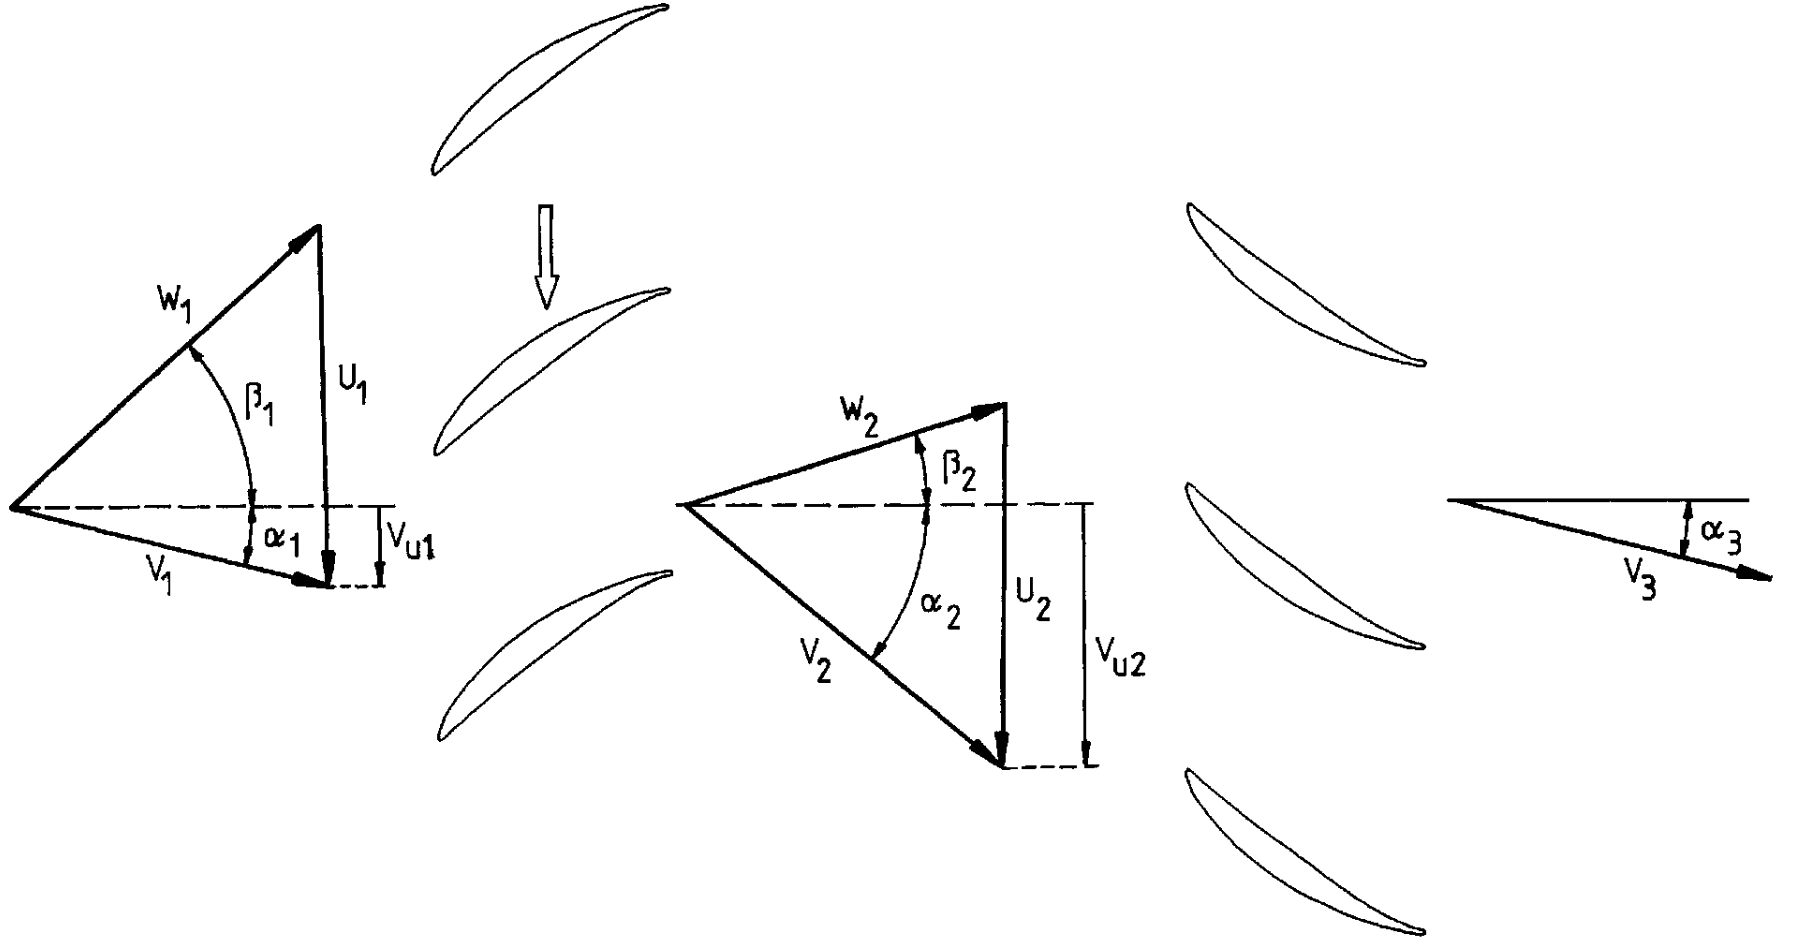
\includegraphics[width=0.5\textwidth]{Comp_stage.png}
    \caption{Axial compressor stage \cite{Hillewaert2019}.}
    \label{fig:C4_compstage}
\end{figure}

The entities between each velocity triangles are the blades of the rotor (emphasized by an arrow) or of the stator. It can be observed that the rotor blades increase the value of the flow velocity \(v\). As explained earlier this augmentation of kinetic energy is then recovered by the stator blades.

\subsubsection{Mollier diagram}
\quad\ The transformation induced by the compressor can be represented into a h-s diagram also named the Mollier diagram. The Mollier diagram for one compressor stage has been drawn in the Figure \ref{fig:C4_Molliercomp}.

\begin{figure}[h]
    \centering
    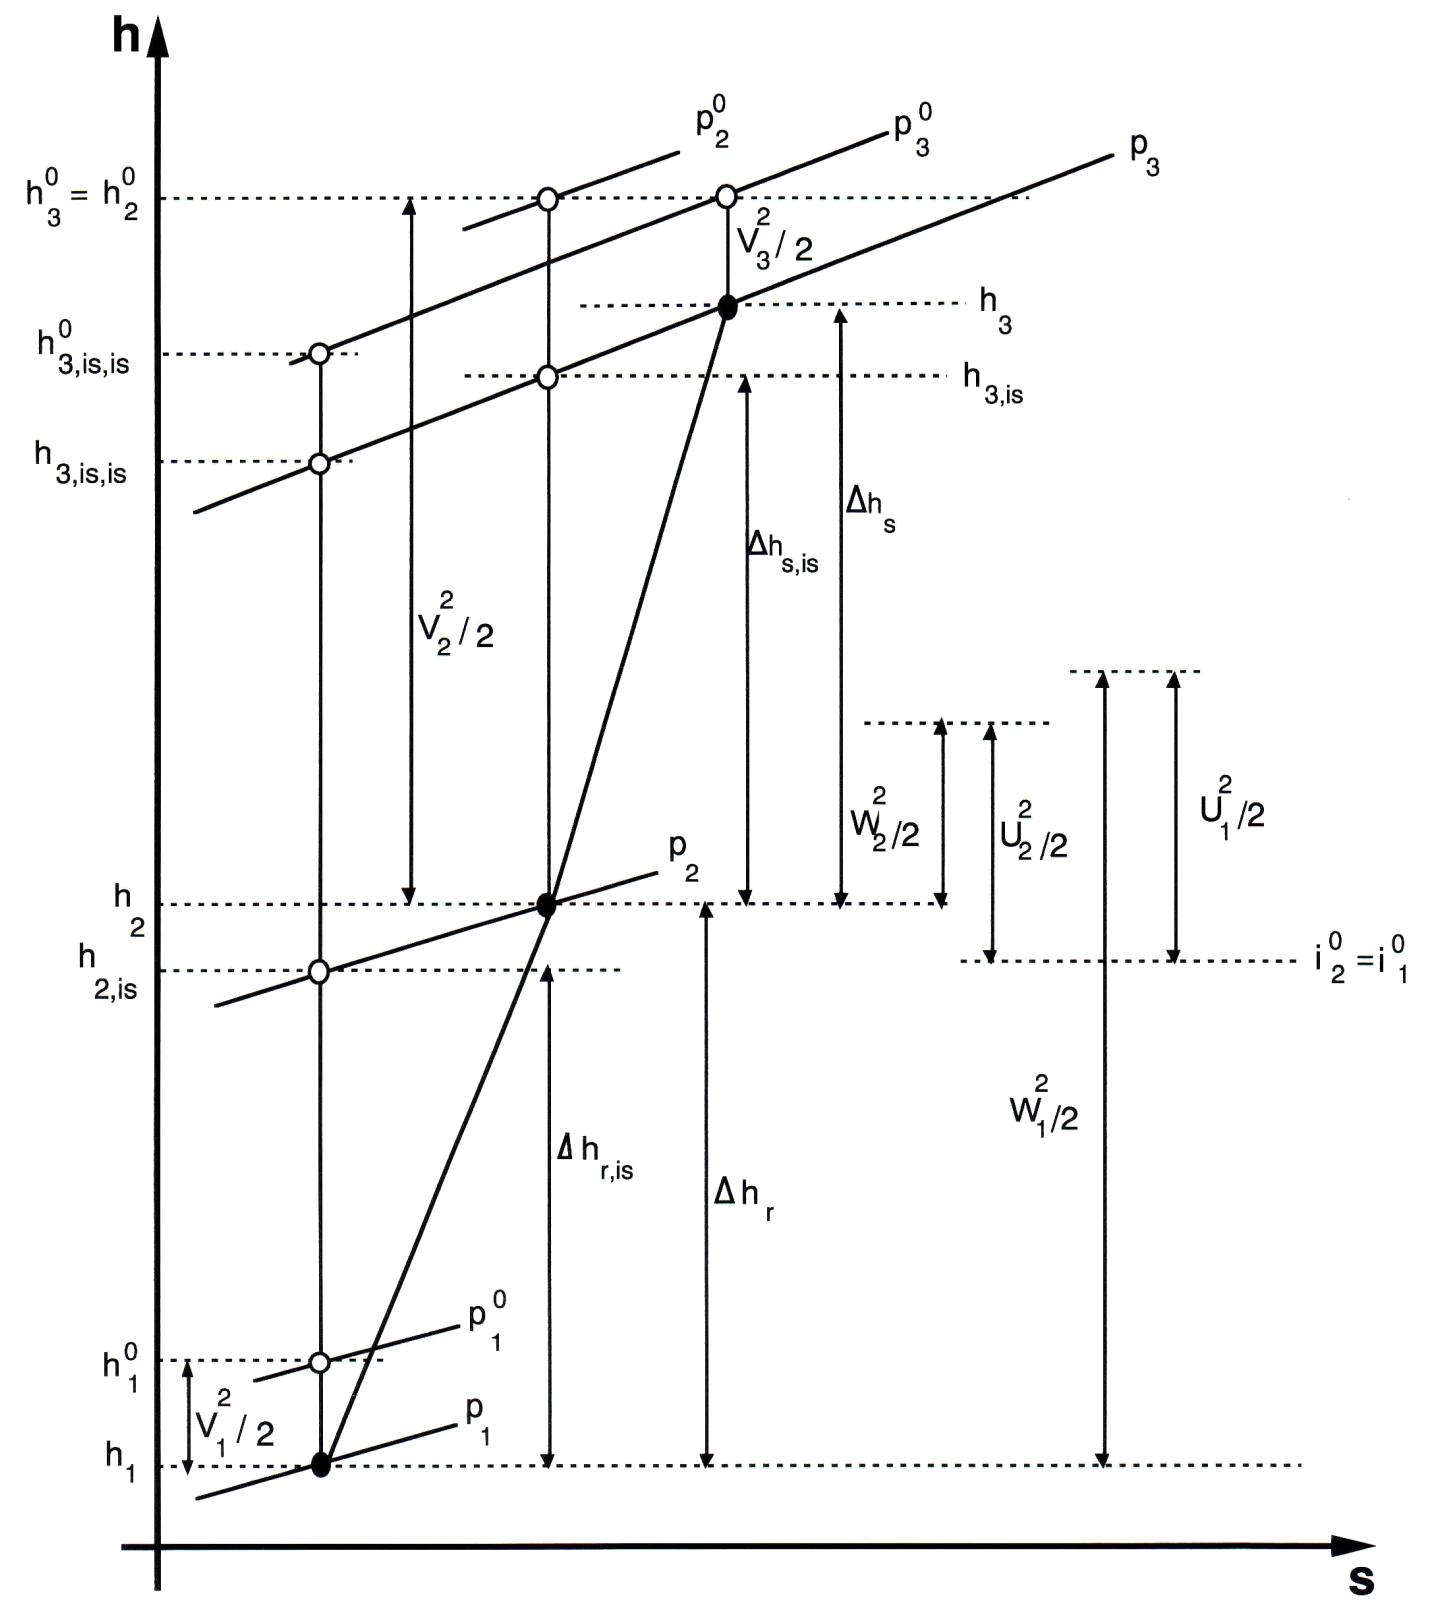
\includegraphics[width=0.5\textwidth]{Comp_mollier.png}
    \caption{Mollier diagram of a compressor stage \cite{Hillewaert2019}.}
    \label{fig:C4_Molliercomp}
\end{figure}

The diagram, for which the velocity triangles are given in the Figure \ref{fig:C4_compstage}, has to be read as follows.
\begin{itemize}
    \setstretch{1}
    \item State \textbf{1}: Starting from the static enthalpy and pressure \(h_1\) and \(p_1\), the relations (\ref{eq:C4_i0}), (\ref{eq:C4_h0}) and (\ref{eq:C4_PP0}) are used to calculate the total enthalpy, rothalpy and pressure.
    \item State \textbf{2}: The transformation \textbf{1}-\textbf{2} takes place within the rotor of the compressor stage. Thus, the total rothalpy is conserved over the transformation ($i_2^0=i_1^0$).

    The knowledge of the total rothalpy allows determining the other quantities. The static enthalpy (and by extension the total enthalpy) can be deduced using the relation (\ref{eq:C4_i0}). Concerning the pressure, there is an increase of the static and total pressure of the fluid ''due to the diffusion in the rotor passage'' ($p_2^{(0)} > p_1^{(0)}$).\cite{Hillewaert2019} 

    \item State \textbf{3}: The transformation \textbf{2}-\textbf{3} takes place within the stator of the compressor stage. Thus, the total enthalpy is conserved over the transformation ($h_3^0 = h_2^0$).

    Then, the static enthalpy can be computed using the relation (\ref{eq:C4_h0}). The conversion of the kinetic energy into pressure leads to an increase of the static and total pressure ($p_3^{(0)} > p_2^{(0)}$).
\end{itemize}
As a reminder, the enthalpy at the end of the process is higher than the one considering an isentropic transformation.
\subsubsection{Performance maps}
\quad\ As for any turbomachines, the compressor can be characterized by its performance map. The map is composed of the performance plot often completed with the efficiency hill. The performance plot provides the total to total pressure ratio \(\Pi_{tt,c}\) as a function of the corrected rotational speed \(N\) and mass flow rate \(\dot{m}_c\).

An illustration of a compressor performance map is given in the Figure \ref{fig:C4_compmap}.
\begin{figure}[h]
    \centering
    \includegraphics[width=0.6\textwidth]{Comp_Map.png}
    \caption{Illustration of a compressor performance map \cite{Dixon2013}.}
    \label{fig:C4_compmap}
\end{figure}

Three types of curve are emphasized on the graph. The solid lines are each associated with one set of operating point characterized by the same corrected rotational speed $N_{corr,c}$. It can be noticed that each iso-rotational speed curve goes asymptotically to the infinity at a given mass flow rate. This value corresponds to the maximal mass flow rate that can go through the compressor and is associated with the phenomenon called choking. 

This maximal mass flow rate $\dot{m}_{choke,c}$ is strongly dependent on the stagnation conditions of the flow. It can be shown that the value of the mass flow rate is proportional to the stagnation pressure and inversely proportional to the square root of the stagnation temperature.

Increasing the rotational speed of the compressor has the effect to increase these stagnation quantities. Since the total pressure increases faster than the total temperature, the maximal flow rate due to the choking will increase with the rotational speed.

Then, there are the doted lines represent the isentropic efficiency contours. These contours produce together what will be called the efficiency hill.

Finally, the red dashed line is called instability line or surge line. The surge line provides a lower bound for the mass flow rate going through the compressor. 

At this minimal flow rate, the flow starts to stall in the machine. Going beyond this limit would lead to a backward flow in the compressor, causing irreversible damages to the compressor. Thus when operating the machine, a certain margin is taken with respect to the surge line.

In the Figure \ref{fig:C4_compmap},  the iso-rotational speed curves start from 70\% to 102.5\% of the nominal rotational speed. This implies that the map is not defined for the operating points characterized by a low rotational speed. This is generally the case for most of the compressor maps.

However, for the low rotational speeds, the flow can be supposed incompressible. Using this approximation, it is possible to use the rules of similarity described in the section about pumps to extrapolate the map to the lower rotational speeds.

\subsection{Gas turbine}
\quad\ From now, only compressor has been introduced. However, in a gas cycle, the compressor is combined with a turbine that will expand the gas. Except in some special configurations, the turbine is always placed after the combustion chamber in a Brayton cycle. This choice allows providing to the turbine a flow with very high enthalpy.

Typically, an axial gas turbine is composed of a stator followed by a rotor. The stator is designed to create a deflection of the flow in the sense of rotation of the rotor. This will accelerate the flow before entering the rotor.

The schematic of an axial turbine stage is drawn in the Figure \ref{fig:C4_turbstage}.
\begin{figure}[h]
    \centering
    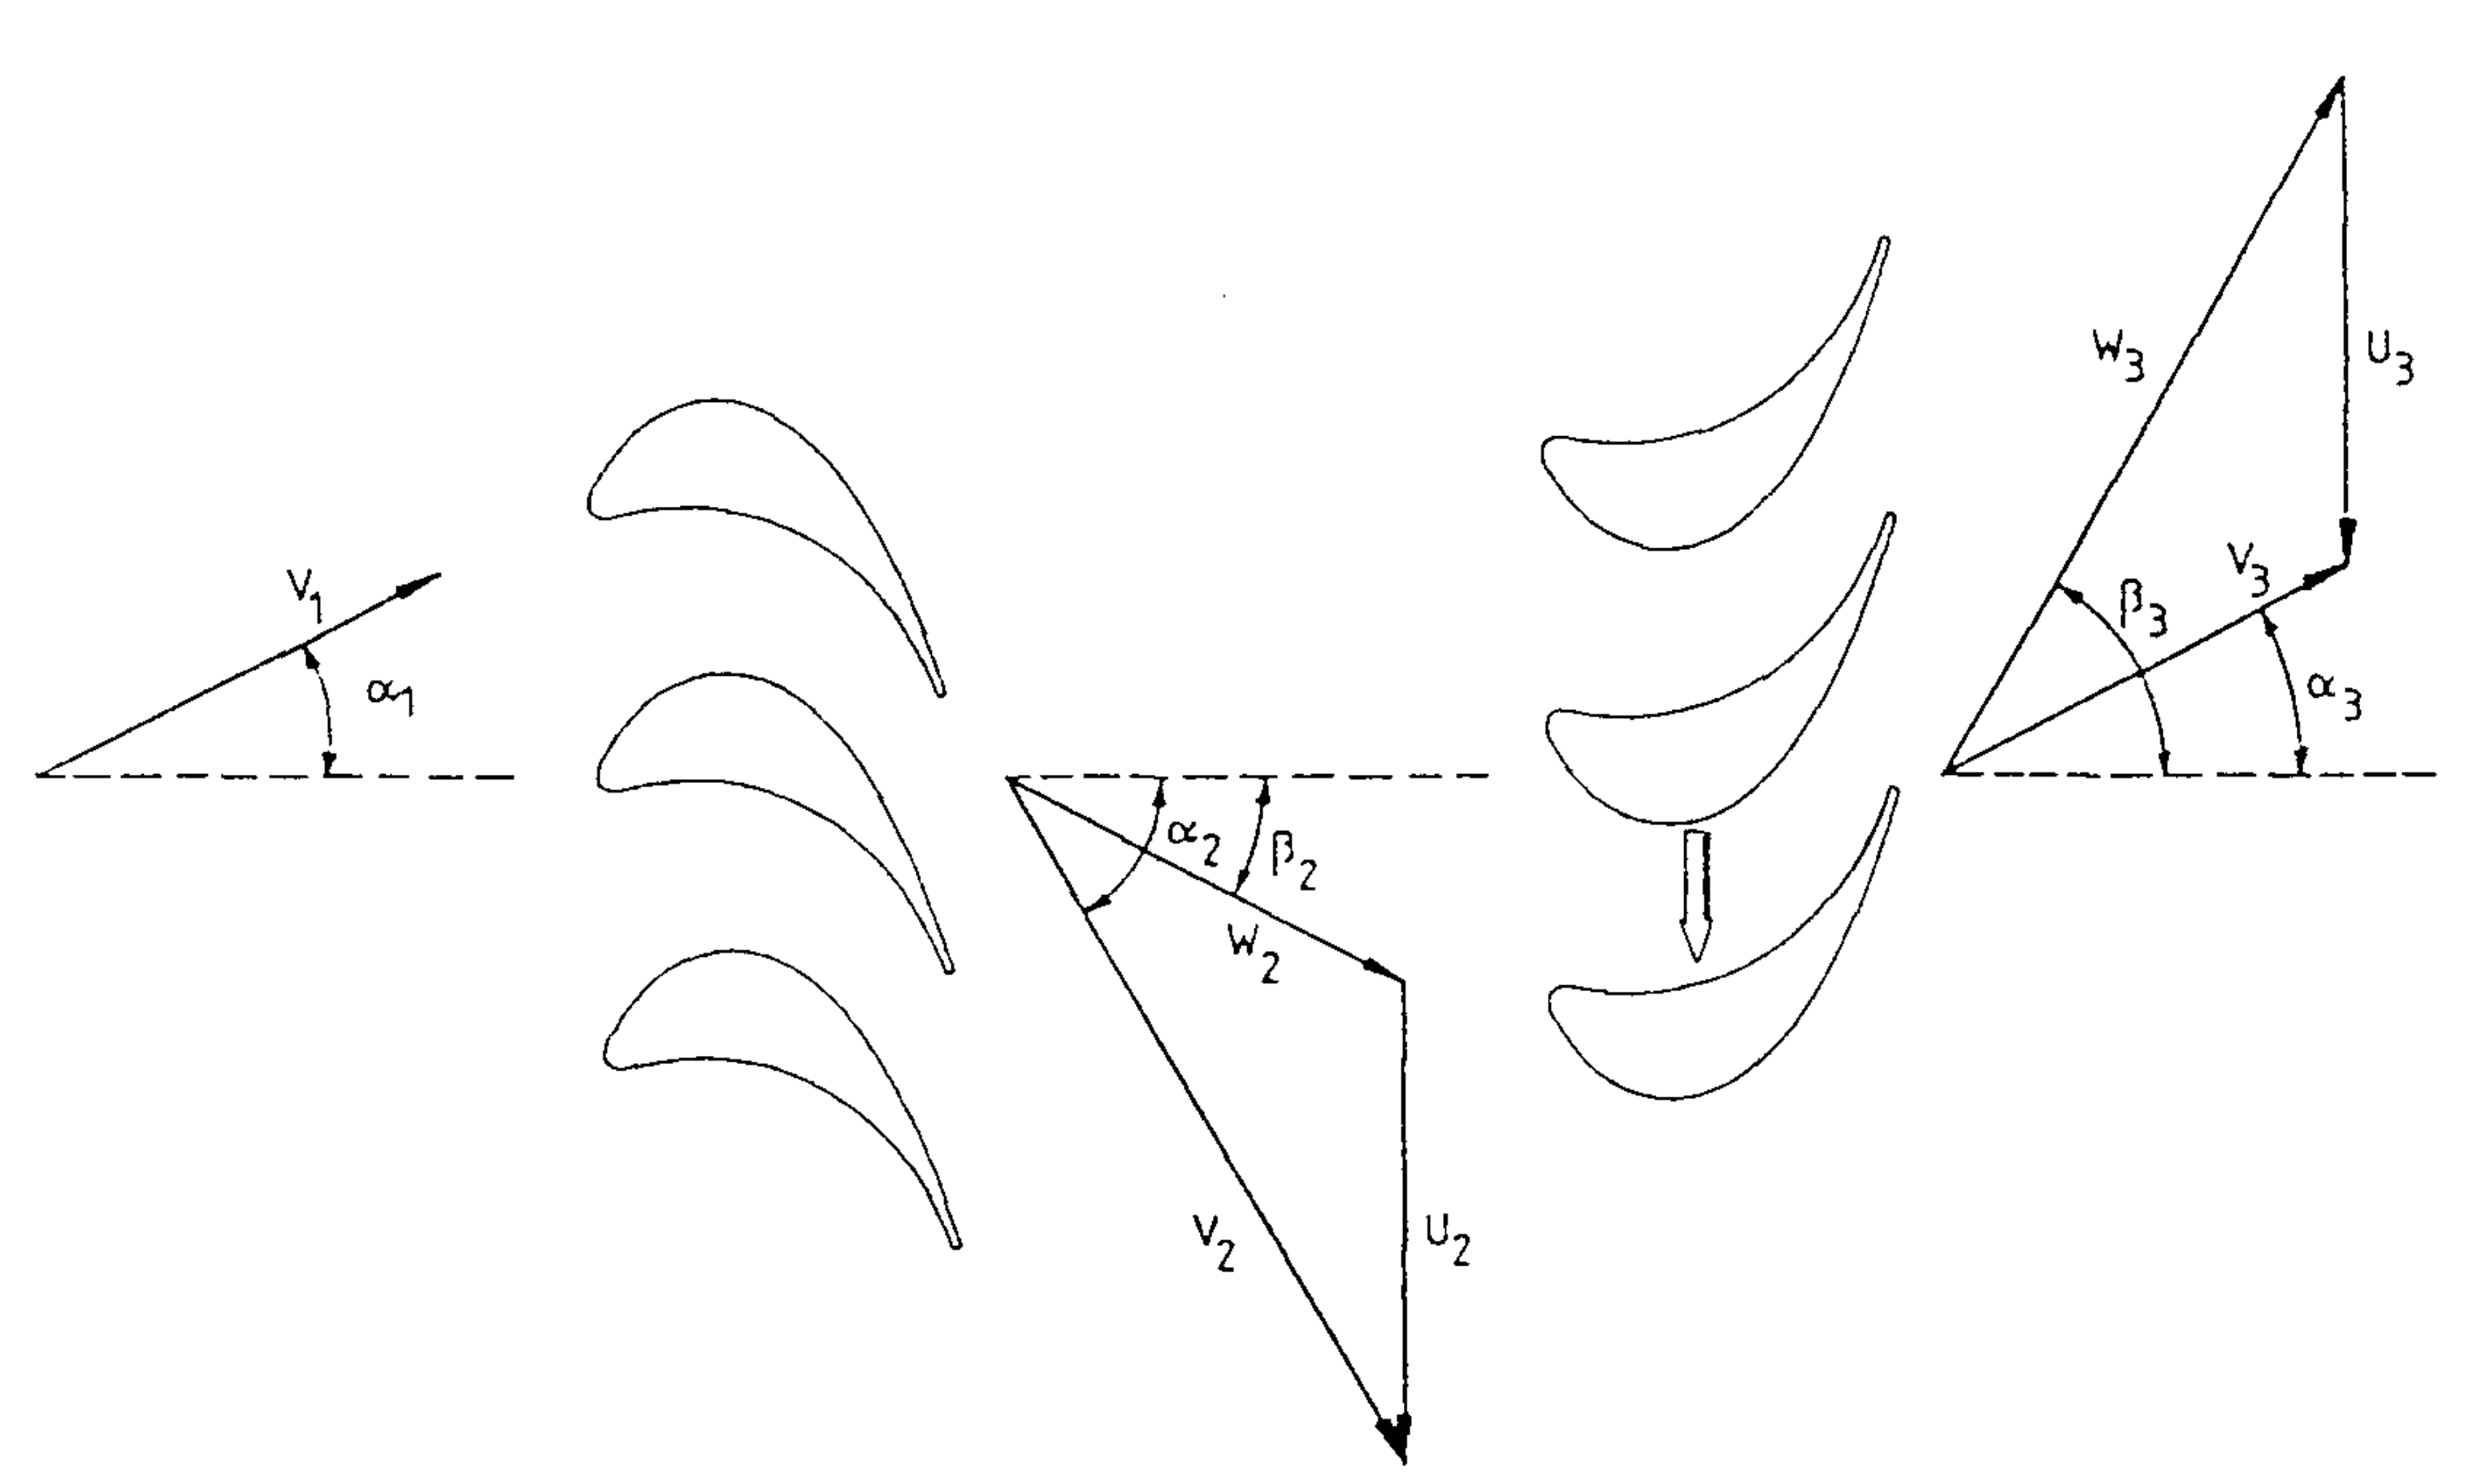
\includegraphics[width=0.5\textwidth]{Turb_stage.png}
    \caption{Axial turbine stage \cite{Hillewaert2019}.}
    \label{fig:C4_turbstage}
\end{figure}\newpage
\subsubsection{Mollier diagram}
As for the compressor, the real expansion induced by the turbine can be represented into a Mollier diagram. The diagram is depicted in the Figure \ref{fig:C4_Mollierturb}. The methodology to read the diagram is the same as before.

\begin{figure}[h]
    \centering
    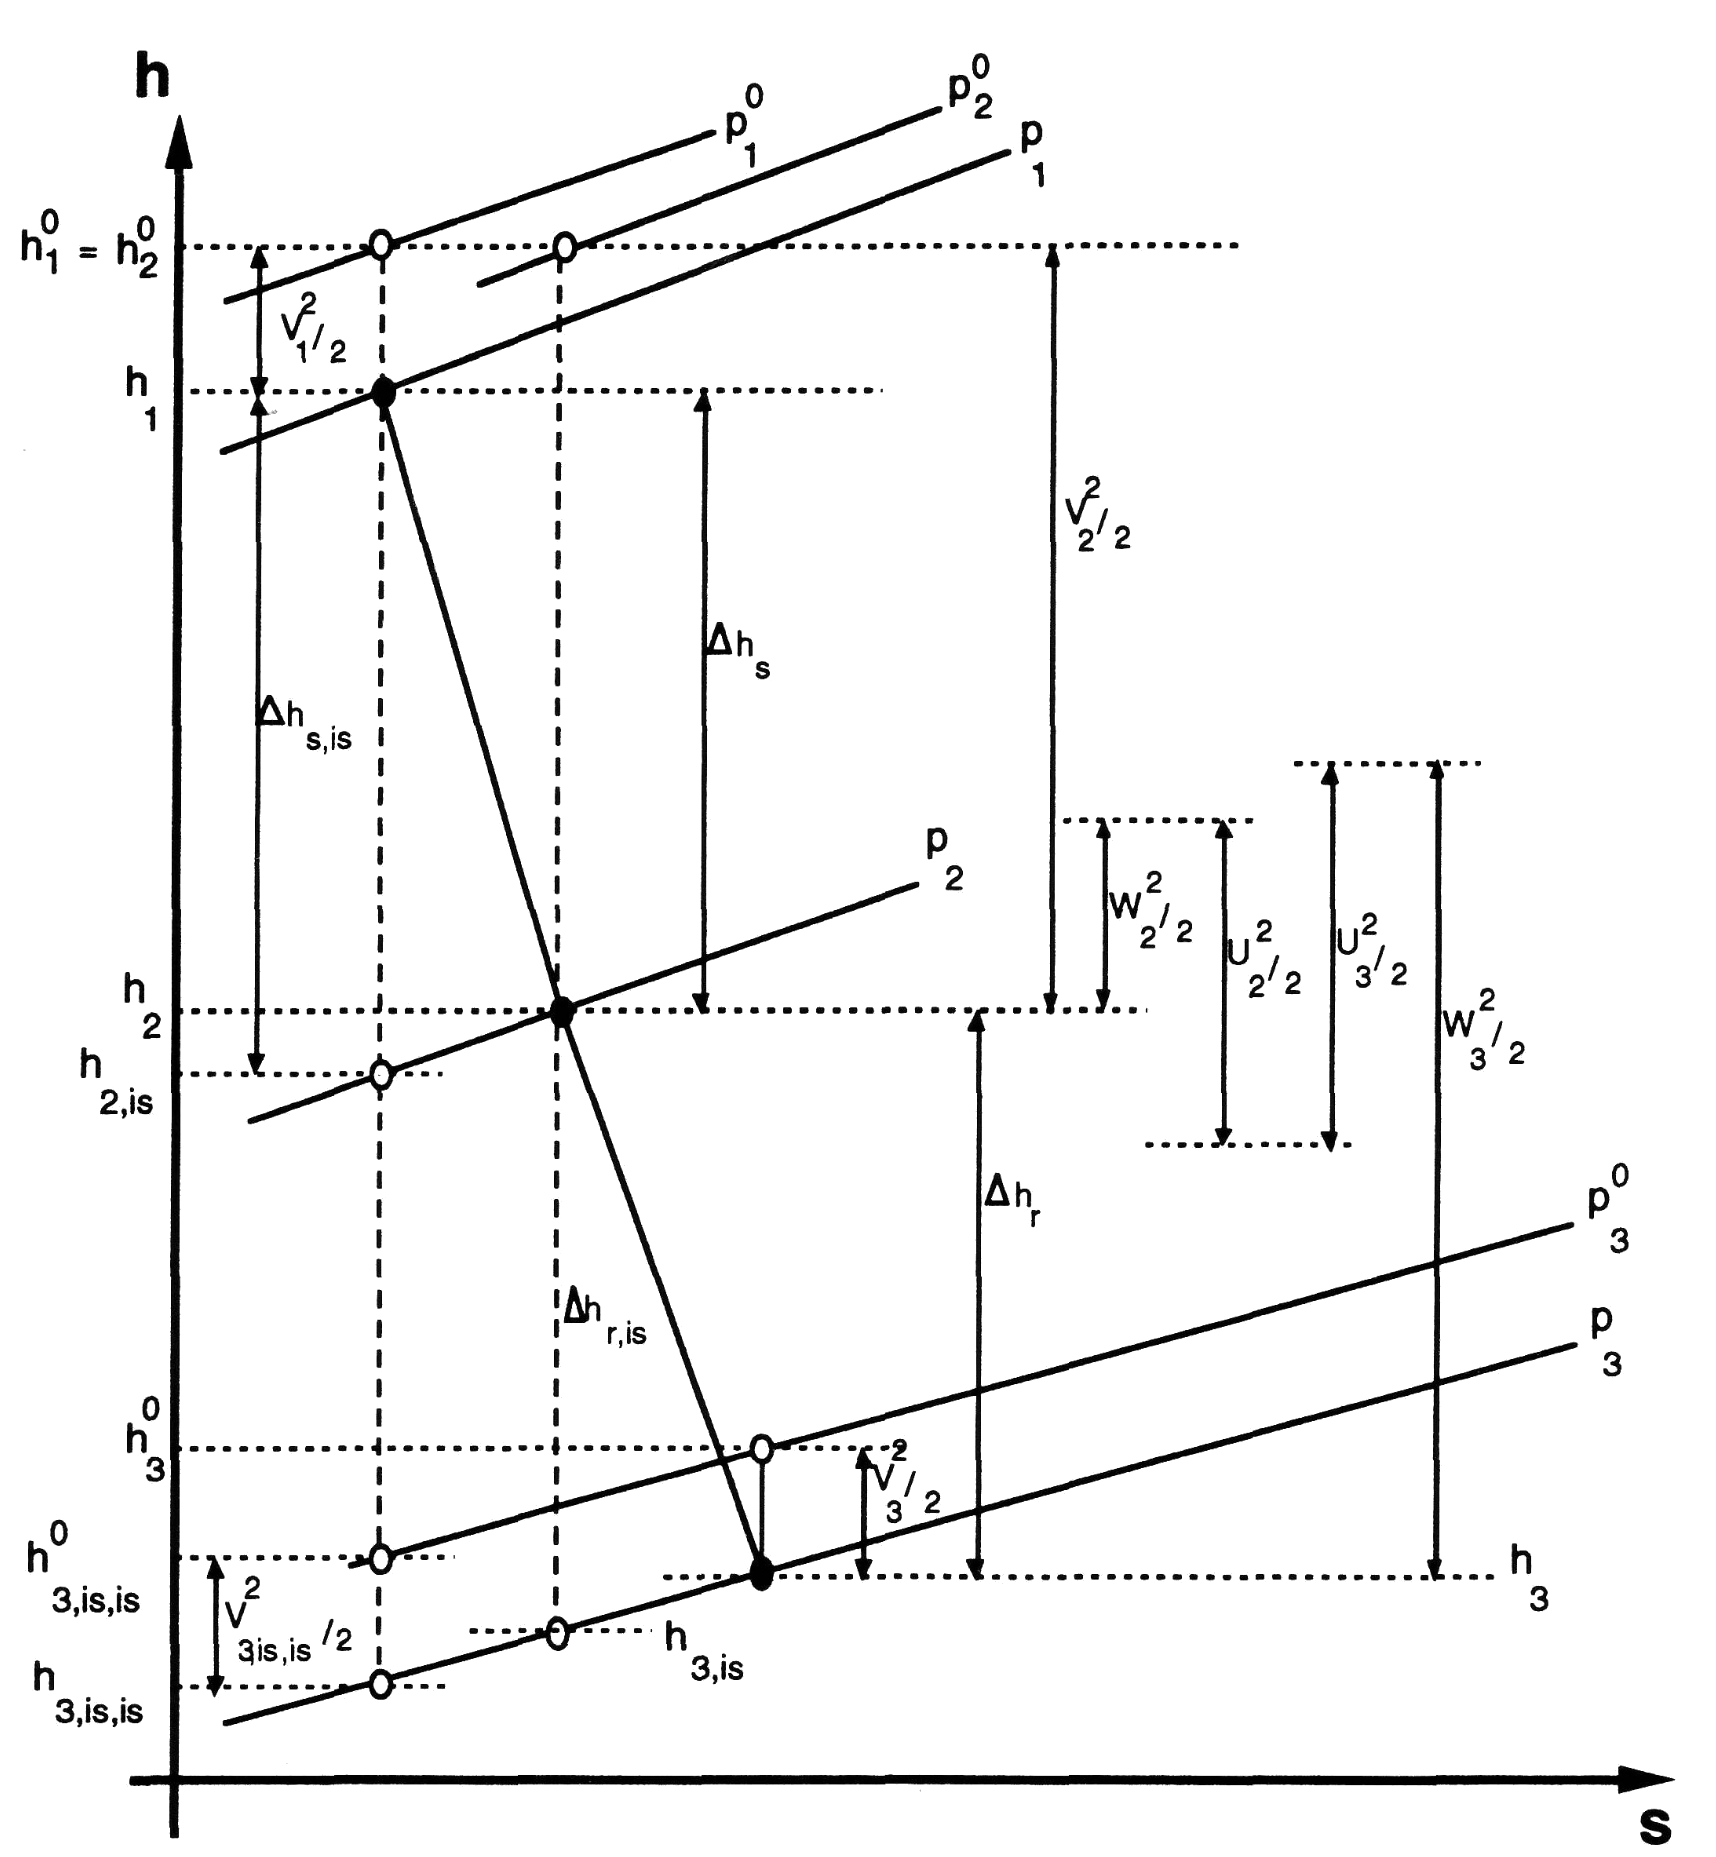
\includegraphics[width=0.5\textwidth]{Turb_mollier.png}
    \caption{Mollier diagram of a turbine stage \cite{Hillewaert2019}.}
    \label{fig:C4_Mollierturb}
\end{figure}

\begin{itemize}
    \setstretch{1}
    \item State \textbf{1}: Starting from the static enthalpy and pressure, the total quantities can be deduced.
    \item State \textbf{2}: The transformation \textbf{1}-\textbf{2} takes place within the stator of the turbine stage. Therefore, the total enthalpy is conserved over the transformation ($h_2^0=h_1^0$).

    Knowing the total enthalpy of the state \textbf{2} allows computing the static enthalpy and by extension the total rothalpy. Plus, since the flow is accelerated by the stator blades, the static and total pressure falls from state \textbf{1} to state \textbf{2} (\(p_2^{(0)}<p_1^{(0)}\)).
    \item State \textbf{3}: The transformation \textbf{2}-\textbf{3} takes place within the rotor of the turbine stage. Therefore, the total rothalpy is conserved over the transformation (\(i_3^0=i_2^0\)).

    Then, the relation (\ref{eq:C4_i0}) allows retrieving the static enthalpy of state \textbf{3}. As shown on the schematic \ref{fig:C4_turbstage} of the turbine stage, the relative speed of the flow is augmented when going through the rotor passage. This generates a second drop of the static and total enthalpy and pressure (\(p_3^{(0)}<p_2^{(0)}\)).

    However, there exists a special stage for which “the relative velocity of the flow to the blade row” of the rotor\cite{Hillewaert2019} remains unchanged, but the flow is inverted. Neglecting the very small variation of the rotor velocity, the static enthalpy and pressure remains unchanged when passing through the rotor.
\end{itemize}




% \subsubsection{Degree of reaction}
% \quad\ The last written paragraph mentioned that some turbines are designed to put all the pressure drop over the stator to limit the axial force generated in the rotor.

% As a general rule, it is possible to classify the turbomachines by creating two categories based on the degree of reaction \(R\). 

% Considering respectively a expansion and compression stage, the degree of reaction is defined as being the ratio between the static enthalpy drop or raise over the rotor and the static enthalpy drop or raise over the turbomachine stage.
% \begin{equation}
%     R = \frac{h_2 - h_3}{h_1 - h_3}\label{eq:C4_R}
% \end{equation}
% From this definition, the two categories can be defined as follows:

% \begin{itemize}
%     \setstretch{1}
%     \item The impulse or action turbomachines: The degree of reaction \(R\simeq 0\). Thus, since the rotor doesn't see any pressure difference, the axial thrust on the shaft is minimized. 
%     \item The reaction turbomachines: The degree of reaction \(R\) is often between 0.5 and 0.7. This means that the pressure drop is distributed between the stator and the rotor.
% \end{itemize}

\subsubsection{Performance maps}
\quad\ The turbines can be also be characterized by a performance map determined from experimental results. The map is often composed of two performance plots as shown in the Figure \ref{fig:C4_turbmap}.

\begin{figure}[h]
    \centering
    \includegraphics[width=0.55\textwidth]{Turb_Map.png}
    \caption{Illustration of a turbine performance map \cite{Dixon2013}.}
    \label{fig:C4_turbmap}
\end{figure}

The two plots in the Figure \ref{fig:C4_turbmap} depict the relations \(\dot{m}_{corr,t}(\Pi_{tt,t},N_{corr,t})\) and \(\eta_{is,t}(\Pi_{tt,t},N_{corr,t})\). 

As it can be noticed in the second diagram, all the curves are all stacked on each other when a certain pressure ratio is reached. Compared to the compressor, the choking phenomenon occurs for the same mass flow rate, regardless the rotational speed considered. 

For a turbine, the expansion is mainly performed within its statoric parts. This massive drop of the total pressure comes with a big increase of the kinetic energy of the flow. 

Therefore, it is within this part of the turbine stage that the choking phenomenon will likely occur. Since the stator is not rotating, the maximal mass flow rate is not really impacted by the rotating speed of the rotor. This is the reason why all the iso-rotational speed curves have the same asymptotic value for the mass flow rate.

To summarize what has been seen in this section about turbomachines, the performance map of the compressor and the turbine
have been introduced thanks to the definition of corrected mass flow rate and rotational speed.

Also, the descriptions of the compression and the expansion have been explained using the h-s Mollier diagrams. Those diagrams, along with the schematic of the compressor and turbine stages, allow describing with a decent accuracy the two previously mentioned transformation.


\section{Combustion chamber}
%%%%%%%%%%%%%%%%%%%%%%%%%%%%%%%%%%%
%%%%%                         %%%%%
%%%%% <<Combustion chamber>>  %%%%%
%%%%%                         %%%%%
%%%%%%%%%%%%%%%%%%%%%%%%%%%%%%%%%%%
\quad\ The previous section introduced the turbomachines. The notion of compressible has been defined, and some important concepts have been emphasized.

In this section, the description of the combustion principle will be considered. Since the study of the fluid mechanic inside the combustion chamber is out of the scope of this work, only combustion equations without dynamic and non-steady effects will be considered.

\subsection{Basis about Chemistry}
\quad\ As it has been mentioned, some combustion reactions will be introduced in this section. Thus, the basic knowledge about chemistry has to be provided.

\subsubsection{Conservation of mass}
During a chemical reaction, the law of conservation of mass (also called the Lavoisier law) has to be satisfied. This implies that the mass of all the reagents combined has to be equal to the mass of the products. An example of chemical reaction is given in (\ref{eq:C4_chem}).

\begin{equation}
    \setstretch{1}
    \underset{\mathrm{16g}}{\ce{1CH4}} \ce{+} \underset{\mathrm{64g}}{\ce{2O2}} \ce{->} \underset{\mathrm{44g}}{\ce{1CO2}} \ce{+} \underset{\mathrm{36g}}{\ce{2H2O}} \ce{+}\text{Heat}\label{eq:C4_chem}
\end{equation}

It will be seen later that this reaction corresponds to the combustion of \textbf{1} mole of methane (\ce{CH4}) using \textbf{2} mole of oxygen (\ce{O2}). The products of the reaction are \textbf{1} mole of \ce{CO2}, \textbf{2} moles of \ce{H2O} and a certain amount of heat transfer to the surroundings. This heat transfer is the desired product of the combustion.

\subsubsection{Conservation of the atomic species}
The second law of conservation states that, during the transformation of the reagent X into the product Y, all the atomic elements from X have to be recovered in Y. For instance, for the equation (\ref{eq:C4_chem}), there is one mole of carbon (\ce{C}) in the reagents. Thus, one mole of \ce{C} has to be present in the products of the reaction.
\newpage
\subsubsection{Proust's law}
The third law to be considered is the Proust law which states that for each chemical reactions, the ratio between the mass of each reagent is a constant. Considering the above example (\ref{eq:C4_chem}), the ratio between the mass of \ce{O2} and \ce{CH4} consumed is given in the equality (\ref{eq:C4_O2CH4mass}).

\begin{equation}
    \setstretch{1}
    \frac{\text{mass of \ce{O2} consumed}}{\text{mass of \ce{CH4} consumed}} = 4 \label{eq:C4_O2CH4mass}
\end{equation}

Let's remark that the law is also valid considering the consumed quantities in mole. In molar quantities, the relation (\ref{eq:C4_O2CH4mass}) becomes (\ref{eq:C4_molratio}).

\begin{equation}
    \setstretch{1}
    \frac{\text{mole of \ce{O2} consumed}}{\text{mole of \ce{CH4} consumed}} = 2  \label{eq:C4_molratio}
\end{equation}

This ratio depends on the type of fuel used. For instance, if the fuel was propane (\ce{C4H8}), the ratio would be equal to 5.

\subsection{Combustion equation}
\quad\ The equation \ref{eq:C4_chem} was illustrating the combustion of the methane \ce{CH4}. The reaction, as written there, supposed that amount of oxygen provided for the reaction is just enough to consume all the methane injected.

This situation, which is the reference, is characterized by an air factor \(\lambda = 1\) (or an excess of air \(e=\lambda-1=0\)). It is said that such combustion is at the stoichiometry.

\subsubsection{Air factor}
The air factor is then defined as being the ratio between

\begin{equation}
    \setstretch{1}
    \lambda = \frac{\varkappa}{\varkappa_{\left.\right|stoichiometry}} \label{eq:C4_lbd}
\end{equation}
Where $\varkappa \doteq \frac{\text{mole of \ce{O2} consumed}}{\text{mole of fuel consumed}}$
Let's note that every other combustive can replaced the oxygen in the relation. However, \ce{O2} is the most common one. Thus, the following development will not consider this possibility.
For the following, the notation \(w_{\ce{\text{<molecules>}}}\) will be used in replacement for ''mole of <molecules> consumed''.

\begin{equation}
    \setstretch{1}
    \lambda = \frac{w_{\ce{O2}}}{2\cdot w_{\ce{CH4}}}\label{eq:C4_lbdCH4}
\end{equation}

For the case of the \ce{CH4} being the fuel, it has been shown in the previous section that the value of the denominator of relation (\ref{eq:C4_lbd}) is equal to 2. Therefore, for this particular combustion, the relation (\ref{eq:C4_lbdCH4}) defines the air factor.



\subsubsection{Generalized combustion equation}
\quad\ As explained, the chemical reaction (\ref{eq:C4_chem}) represents the ideal case with an air factor of 1. Also, it is considered that the combustive is pure \ce{O2}. In reality, the used reagent for the combustion is ambient air which is composed of 21\% of \ce{O2} and 79\% of nitrogen (\ce{N2}).

Thus, the generalized combustion equation (for the \ce{CH4}) is defined as in the reaction (\ref{eq:C4_chemgeng0}).

\begin{equation}
    \setstretch{1}
    \ce{CH4 +}2\lambda \left(\ce{O2}+\frac{79}{21}\ce{N2}\right) \ce{-> CO2 + 2(\lambda-1)O2 + 2H2O + 2\lambda\frac{79}{21}N2 + \text{Heat}}\label{eq:C4_chemgeng0}
\end{equation}

This equation, while being correct for any values of \(\lambda\) greater or equal than 1, has to be modified to take into account the event for which the excess of air \(e\) is lower than zero (with \(e=\lambda -1\)). For such values, the combustion equation then becomes as stated in (\ref{eq:C4_chemgeng1}).

\begin{equation}
    \setstretch{1}
    \ce{CH4 +}2\lambda \left(\ce{O2}+\frac{79}{21}\ce{N2}\right) \ce{-> aCO2 + bCO + 2H2O + 2\lambda\frac{79}{21}N2 + \text{Heat}}\label{eq:C4_chemgeng1}
\end{equation}

Where coefficients ''a'' and ''b'' satisfies the system (\ref{eq:C4_sysab}).

\begin{equation}
    \setstretch{1}
    \begin{cases}
        \text{a} + \text{b} = 1 \\
        2\text{a} + \text{b} = 4\lambda - 2
    \end{cases}\label{eq:C4_sysab}
\end{equation}

Both equations have been obtained based on the conservation of the atomic species. It can be calculated that there exists a lower bound for the air factor below which the combustion will be impossible. The condition is that the coefficient ''a'' cannot be smaller than zero. For this case, the minimal air factor \(\lambda_{min} =-\frac{3}{4}\).

To provide some definitions, the mixture \ce{O2}-fuel is said poor when \(\lambda>1\), rich when \(\lambda<1\) and at the stoichiometry for an air factor \(\lambda=1\). Typically, for a gas turbine the mixture is very poor with a $\lambda$ often greater than 4-5.

\subsection{Fuel characteristic}
\quad\ From now, the amount of heat provided during the combustion has not been quantified. This quantification is really important because this amount of heat is linked to quality and the nature of the fuel.

\subsubsection{Heating calorific value}
\quad\ First, let's define the heating calorific value \(HCV\) of a fuel (J/kg). By definition, it is ''the amount of thermal energy released during the total combustion of one physical unit of fuel” \cite{Leonard2018}.

\begin{equation}
    \setstretch{1}
    HCV = -\Delta H^o_{combustion} \label{eq:C4_HCV1}
\end{equation}

With \(-\Delta H^o_{combustion}\) being the heat released during the reaction.

The \(HCV\) is determined at a given reference temperature \(T_0\). Considering this reference temperature, the \(HCV\) can be evaluated by computing the enthalpy difference between the reagents and the products.

\begin{equation}
    \setstretch{1}
    HCV = h_{reagent\left.\right|T=T_0} - h_{product\left.\right|T=T_0}\label{eq:C4_HCV2}
\end{equation}

Distinction between the lower and higher heating calorific value (respectively $HCV_l$ and $HCV_h$) have to be made. Basically, when considering the combustion of a given fuel, the amount of energy released corresponds to the lower heating calorific value if the water remains gaseous within the exhaust gas. 

However, when the water contained in the exhaust gas have been condensed into liquid water, the energy released from the phenomenon is added to the lower $HCV$. For this case, the higher heating calorific value is then used instead of the lower one. In this work, only lower heating calorific value will be considered since the condensation of the water will be taken into account.

The \(HCV\) value depends on the type of fuel that is used. For example, the lower heating calorific value of the \ce{CH4} is around 50 MJ/kg.


\subsubsection{Adiabatic flame temperature}
\quad\ The second notion that can be defined is the adiabatic flame temperature \(T_f\). If the combustion chamber is supposed to be adiabatic (no heat transfer to the outside), the heat generated will be fully retained within the exhaust gas of the combustor. Thus, the temperature reached by the gas is considered to maximal and is called the adiabatic flame temperature.

The evaluation of the temperature \(T_f\) is quite similar to the one of the \(HCV\). Here, starting from the reference temperature, the temperature \(T_f\) is calculated such that the enthalpy of the products is equal to the enthalpy of the reagents.

\begin{equation}
    \setstretch{1}
    h_{reagent\left.\right|T=T_0} = h_{product\left.\right|T=T_f}\label{eq:C4_T_f}
\end{equation}

\subsubsection{Combustion efficiency}
\quad\ The combustion efficiency is defined as being the ratio between the heat injected into the combustion chamber the heat that can be \textit{used} for the combustion. This is expressed in the relation (\ref{eq:C4_etaCC}).

\begin{equation}
    \setstretch{1}
    \eta_{cc} = \frac{\dot{Q}}{\dot{m}_{Fuel}\cdot HCV_{Fuel}}\label{eq:C4_etaCC}
\end{equation}
\subsection{Fumes composition}
\quad\ Previously has been presented in the equations (\ref{eq:C4_chemgeng0}) and (\ref{eq:C4_chemgeng1}) the generalized chemical reaction for the combustion of the methane.
In a more general case, the fuel is essentially composed of carbon \ce{C}, hydrogen \ce{H}, oxygen \ce{O} and nitrogen \ce{N} in some proportion. Therefore, the reactions (\ref{eq:C4_chemgeng0}) and (\ref{eq:C4_chemgeng1}) can be reformulated taking into account a general composition for the fuel.

\begin{subequations}
    \setstretch{1}
 \begin{align}
     \ce{C_{\text{m}}H_{\text{n}}O_{\text{x}}N_{\text{y}} +}\kappa\lambda \left(\ce{O2}+\frac{79}{21}\ce{N2}\right) &\ce{-> mCO2 +} \kappa(\lambda-1)\ce{O2 + \frac{n}{2}H2O +} (\kappa\lambda\frac{79}{21} + \frac{\text{y}}{2})\ce{N2}\\
     \text{ for \(\lambda\geq 1\)}\nonumber\\
     \ce{C_{\text{m}}H_{\text{n}}O_{\text{x}}N_{\text{y}} +}\kappa\lambda \left(\ce{O2}+\frac{79}{21}\ce{N2}\right) &\ce{-> aCO2 + bCO + \frac{n}{2}H2O} + (\kappa\lambda\frac{79}{21} + \frac{\text{y}}{2})\ce{N2}\\
     \text{ for \(\lambda< 1\)}\nonumber
 \end{align}
        \label{eq:C4_chemgeng01}
\end{subequations}

where coefficients ''a'' and ''b'' satisfies the system (\ref{eq:C4_sysab2})

\begin{equation}
    \setstretch{1}
    \begin{cases}
        \text{a} + \text{b} = \text{m} \\
        2\text{a} + \text{b} = 2\kappa\lambda + \frac{\text{x}}{2} - \frac{\text{n}}{2}
    \end{cases}\label{eq:C4_sysab2}
\end{equation}

With the factor \(\kappa = (\text{m}+\frac{\text{n}}{4}-\frac{\text{x}}{2})\). The coefficients ''m'' and ''n'' correspond to the number of moles of atoms of carbon and hydrogen within one mole of fuel.

From theses equations, it is possible to obtain the molar fraction \(x_i\) of each fume components. By definition, the molar fraction of the component \(i\) is the ratio between the number of moles \(n_i\) of the component \(i\) and the total number of moles \(n_{tot}\), all species taken together.

\begin{equation*}
    \setstretch{1}
    x_i = \frac{n_i}{n_{tot}}
\end{equation*}

From the molar fraction, the mass fraction can be obtained using the formula (\ref{eq:C4_x2y})

\begin{equation}
    \setstretch{1}
    y_i = x_i\frac{MM_{tot}}{MM_i} \label{eq:C4_x2y}
\end{equation}

Where \(MM_i\) is the molar mass (in g/mol) of the component \(i\) and \(MM_{tot}\) is the total molar mass of the fumes. The total molar mass of the fumes is obtained as stated in the relation (\ref{eq:C4_MMtot}).

\begin{equation}
    \setstretch{1}
    MM_{tot} = \sum_i x_i\cdot MM_i \label{eq:C4_MMtot}
\end{equation}

This method will be called the ''weight factor'' method.

\section{Heat-exchangers}
%%%%%%%%%%%%%%%%%%%%%%%%%%%%%%%%%%%
%%%%%                         %%%%%
%%%%%   <<Heat-exchanger>>    %%%%%
%%%%%                         %%%%%
%%%%%%%%%%%%%%%%%%%%%%%%%%%%%%%%%%%
\quad\ The last important component that has to be defined and characterized is the heat exchanger (HX). As the name says, the purpose of this element is to transfer the heat from a \textbf{hot} fluid to a \textbf{cold} fluid. The heat-exchangers can be classified into several categories\cite{Ngendakumana2018}.

\begin{itemize}
    \setstretch{1}
    \item The recuperators: Their purpose is to recover the heat from a hot fluid to heat up a cold fluid for direct usage. For instance, the exhaust gas from a boiler will go through a recuperator to exchange its energy with water. For this application and for many others, the two streams within the HX are separated by physical walls.

    Alternatively, the heat exchange can be performed by direct contact between the two fluids. In this case, nothing prevents the hot flow from mixing with the cold flow (and vice versa).
    \item The regenerators: For a given cycle , the purpose of the regenerators is to use a hot flow from the cycle to heat up a cold flow from the same cycle.
\end{itemize}

By definition, the hot stream is the one that \textbf{provides} the heat, and the cold stream is the one \textbf{receiving} the heat.

\begin{figure}[h]
    \centering
    \subfloat[HX with fined plates.\label{fig:C4_HX_fin_plate}]
    {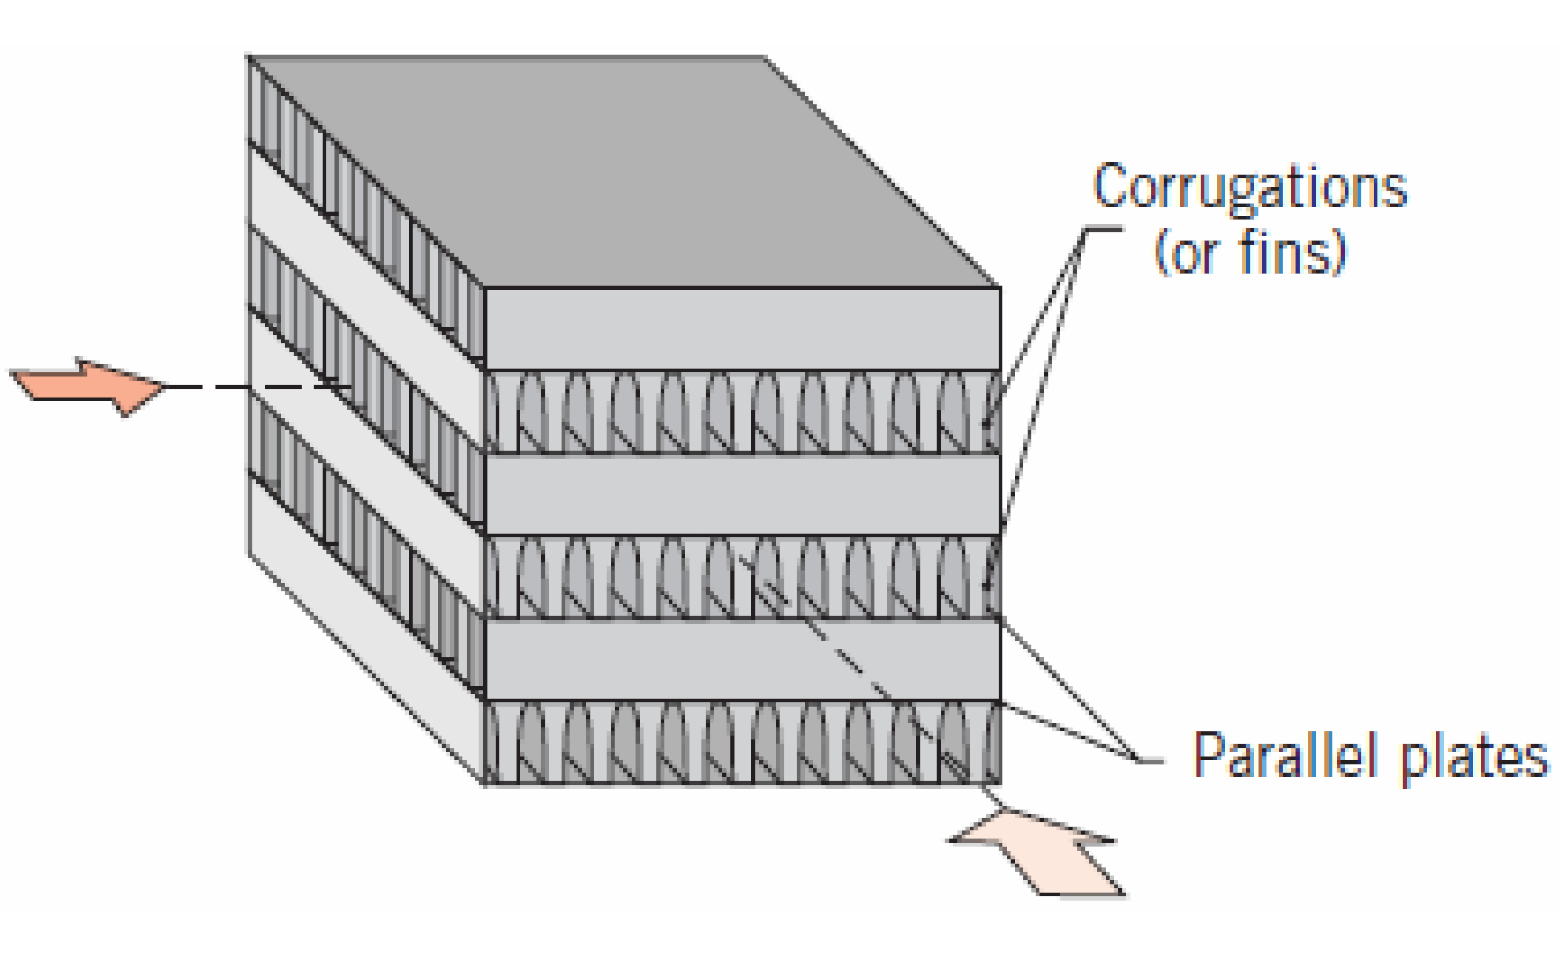
\includegraphics[width=0.3\textwidth]{HX_fin_plate}}\hfill
    \subfloat[HX with fined tubes.\label{fig:C4_HX_fin_tube}]
    {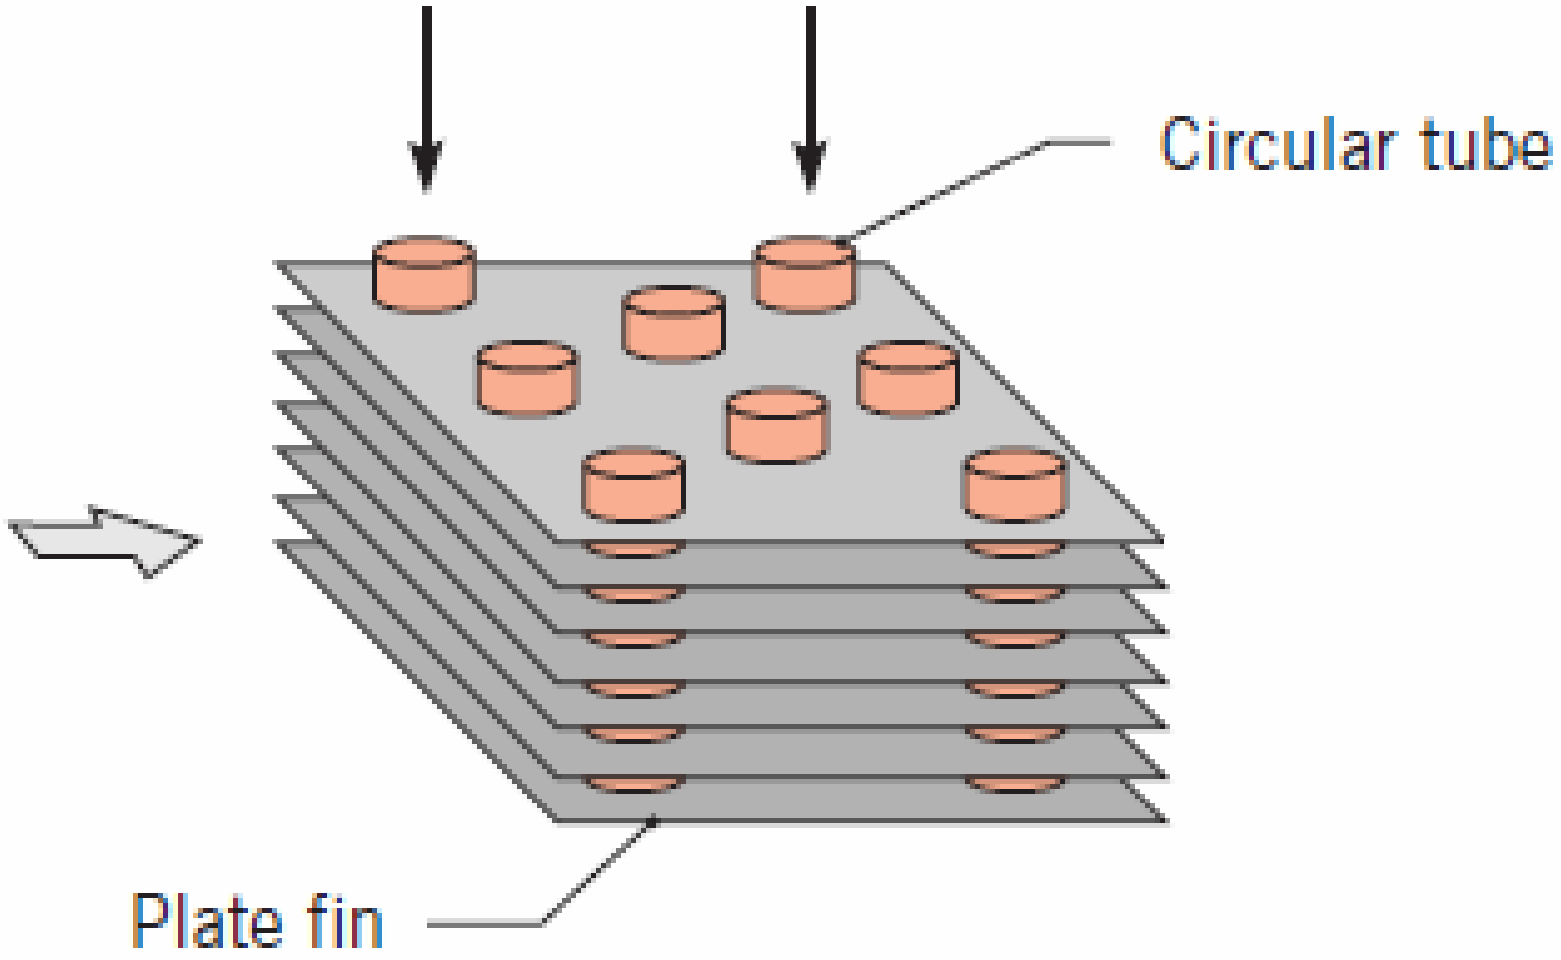
\includegraphics[width=0.3\textwidth]{HX_fin_tube}}\hfill
    \subfloat[Plate heat exchangers.\label{fig:C4_PHE}]
    {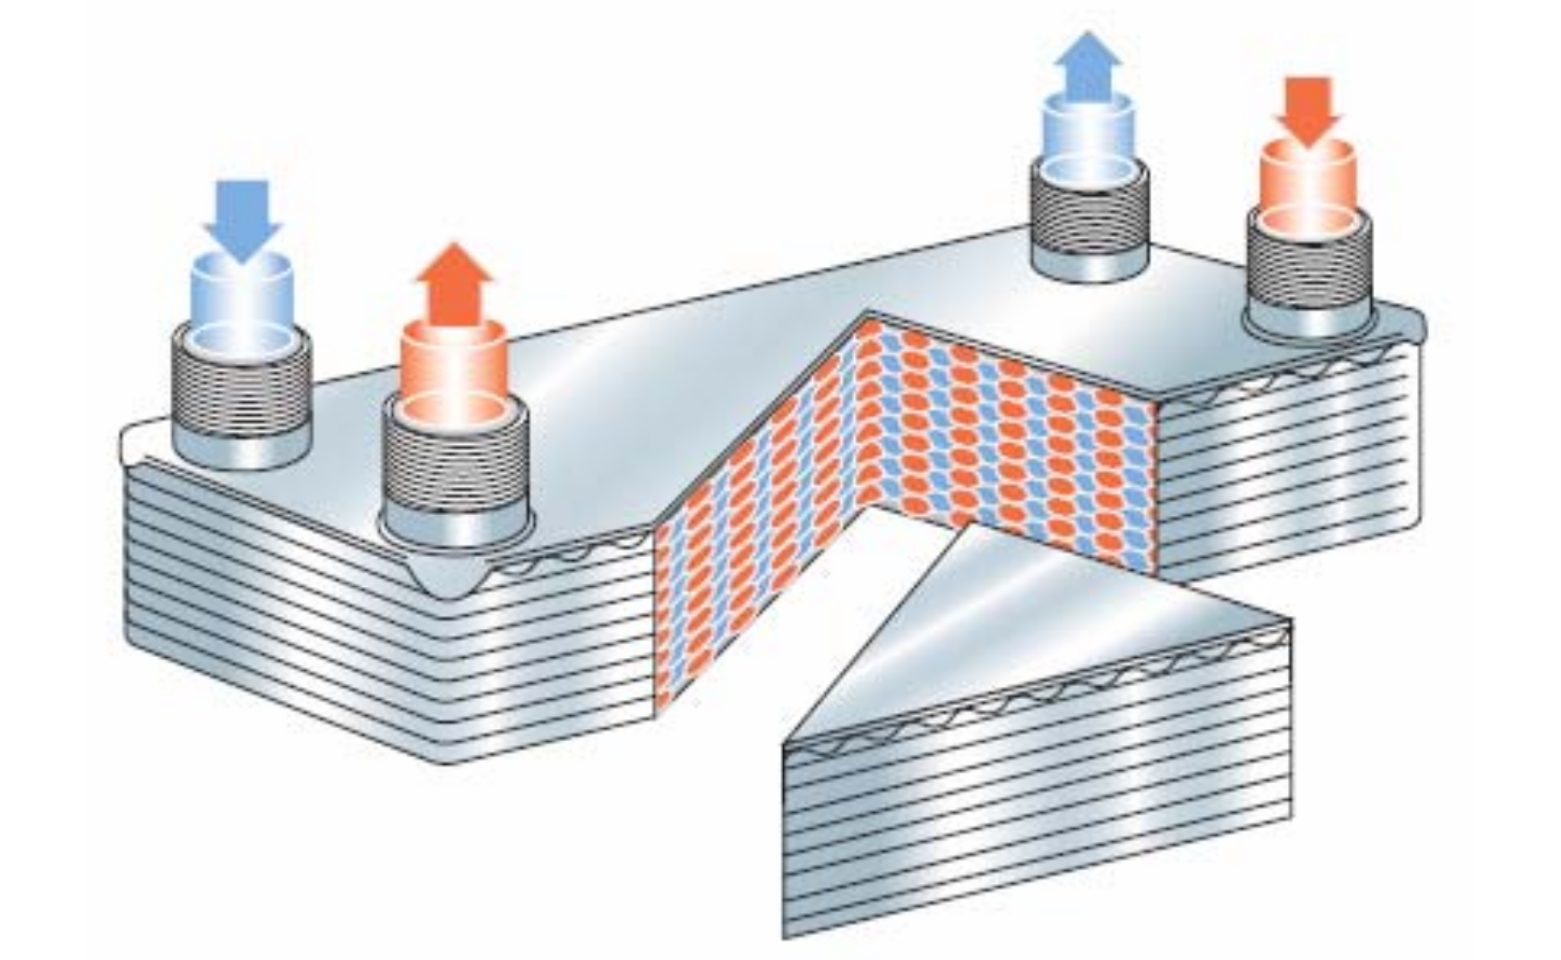
\includegraphics[width=0.3\textwidth]{HX_brased_plate}}
    \caption{HX illustrations \cite{Ngendakumana2018}.} \label{fig:C4_HX}
\end{figure}

In the Figure \ref{fig:C4_HX} are depicted some illustrations of heat exchanger owning at different families.
The selected family will highly depends on the type of application that is targeted. Plate heat exchangers are one of the most compact types of heat exchangers. This compactness is highly appreciated for any system where the foot print and volume have to be as minimal as possible. However, this is at the cost of more complicated maintenance due to the brazing of the plates.

This section will not cover the specificity of these different families. Instead, the main notions which are necessary to characterize the heat transfer between two fluids will be given.

\subsection{Stream configurations}
\quad\ There isn't a unique configuration regarding about the interaction between the hot and cold streams. Indeed, here are the main categories based on flow configurations.

\begin{itemize}
    \setstretch{1}
    \item Parallel flow HX: The two streams go through the heat exchanger in the same direction (Figure \ref{fig:C4_para_flow}).

    \item Counter flow HX: The two streams go through the heat exchanger in the opposite direction. This configuration is more frequent than the parallel flow HX due to higher efficiency. However, sometimes the network of piping doesn't permit installing such configuration (Figure \ref{fig:C4_counter_flow}).

    \item Cross flow HX, both fluids unmixed: The flow in the tube does not see the property of cross flow varying along with the distance traveled. Both flows are unmixed (Figure \ref{fig:C4_cross_flow_unmixed}).
  
    \item Cross flow HX, one fluid mixed: The flow in the tube does not see the property of cross flow varying along with the distance traveled. The cross flow does not travel inside isolated channels (Figure \ref{fig:C4_cross_flow_1mixed}).
\end{itemize}
\begin{figure}[h]
        \centering
    \subfloat[Parallel flow heat exchanger.\label{fig:C4_para_flow}]
    {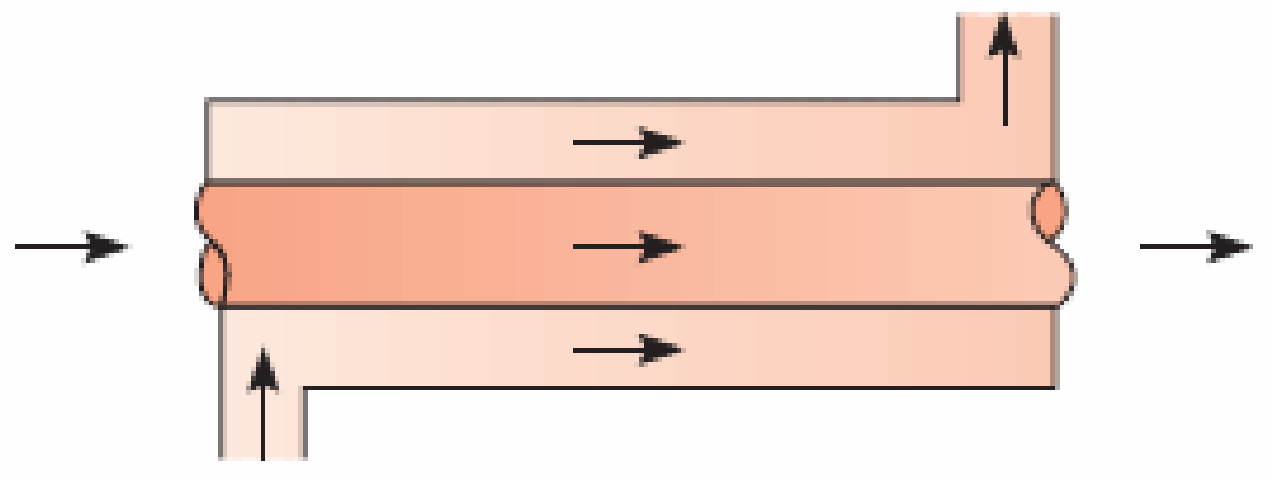
\includegraphics[width=0.3\textwidth]{parallele_flow}}\hfill
    \subfloat[Counter flow heat exchanger.\label{fig:C4_counter_flow}]
    {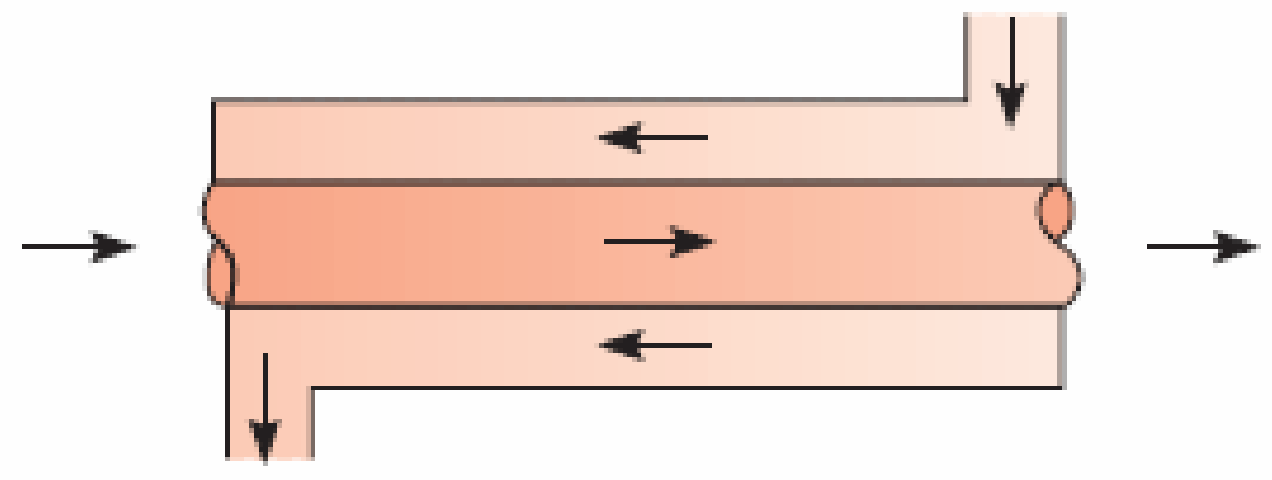
\includegraphics[width=0.3\textwidth]{opposite_flow}}\hfill
    \subfloat[Cross flow heat exchanger, both fluids unmixed.\label{fig:C4_cross_flow_unmixed}]
    {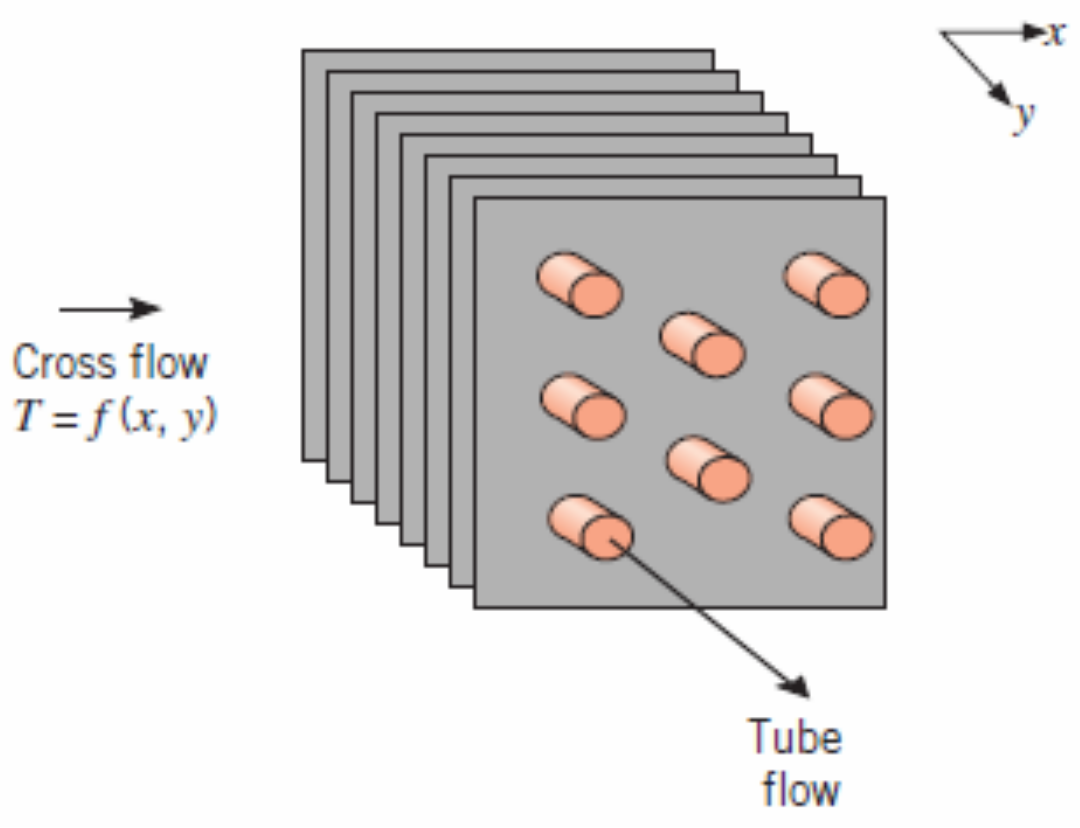
\includegraphics[width=0.3\textwidth]{crossed_flow_non_mixed}}\hfill
    \subfloat[Cross flow heat exchanger, one fluid mixed.\label{fig:C4_cross_flow_1mixed}]
    {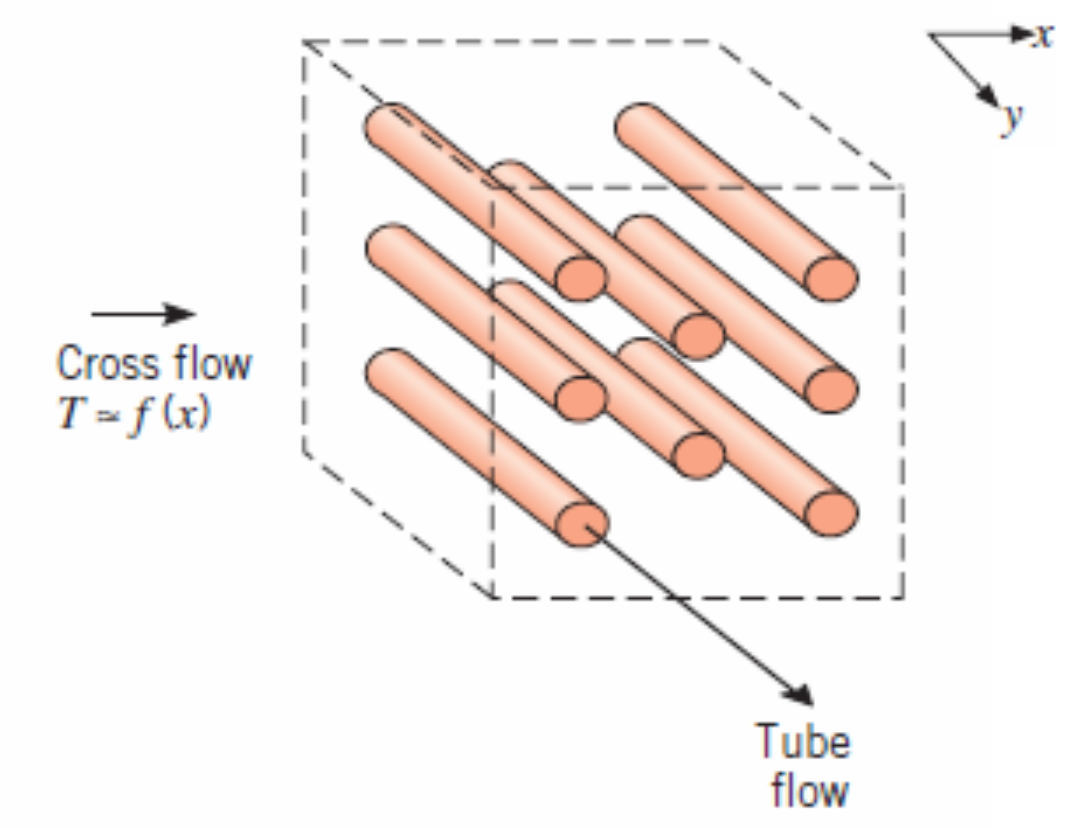
\includegraphics[width=0.3\textwidth]{crossed_flow_one_mixed}}
    \caption{Configurations of heat exchangers\cite{Ngendakumana2018}.} \label{fig:C4_config}
\end{figure}
Considering the parallel and counter flow heat exchanger, two temperature differences can be defined based on the temperature profiles (Figure \ref{fig:C4_Tprof}) of both fluids inside the heat exchanger.

\begin{figure}[h]
    \centering
    \begin{subfigure}[b]{0.45\textwidth}
        \centering
        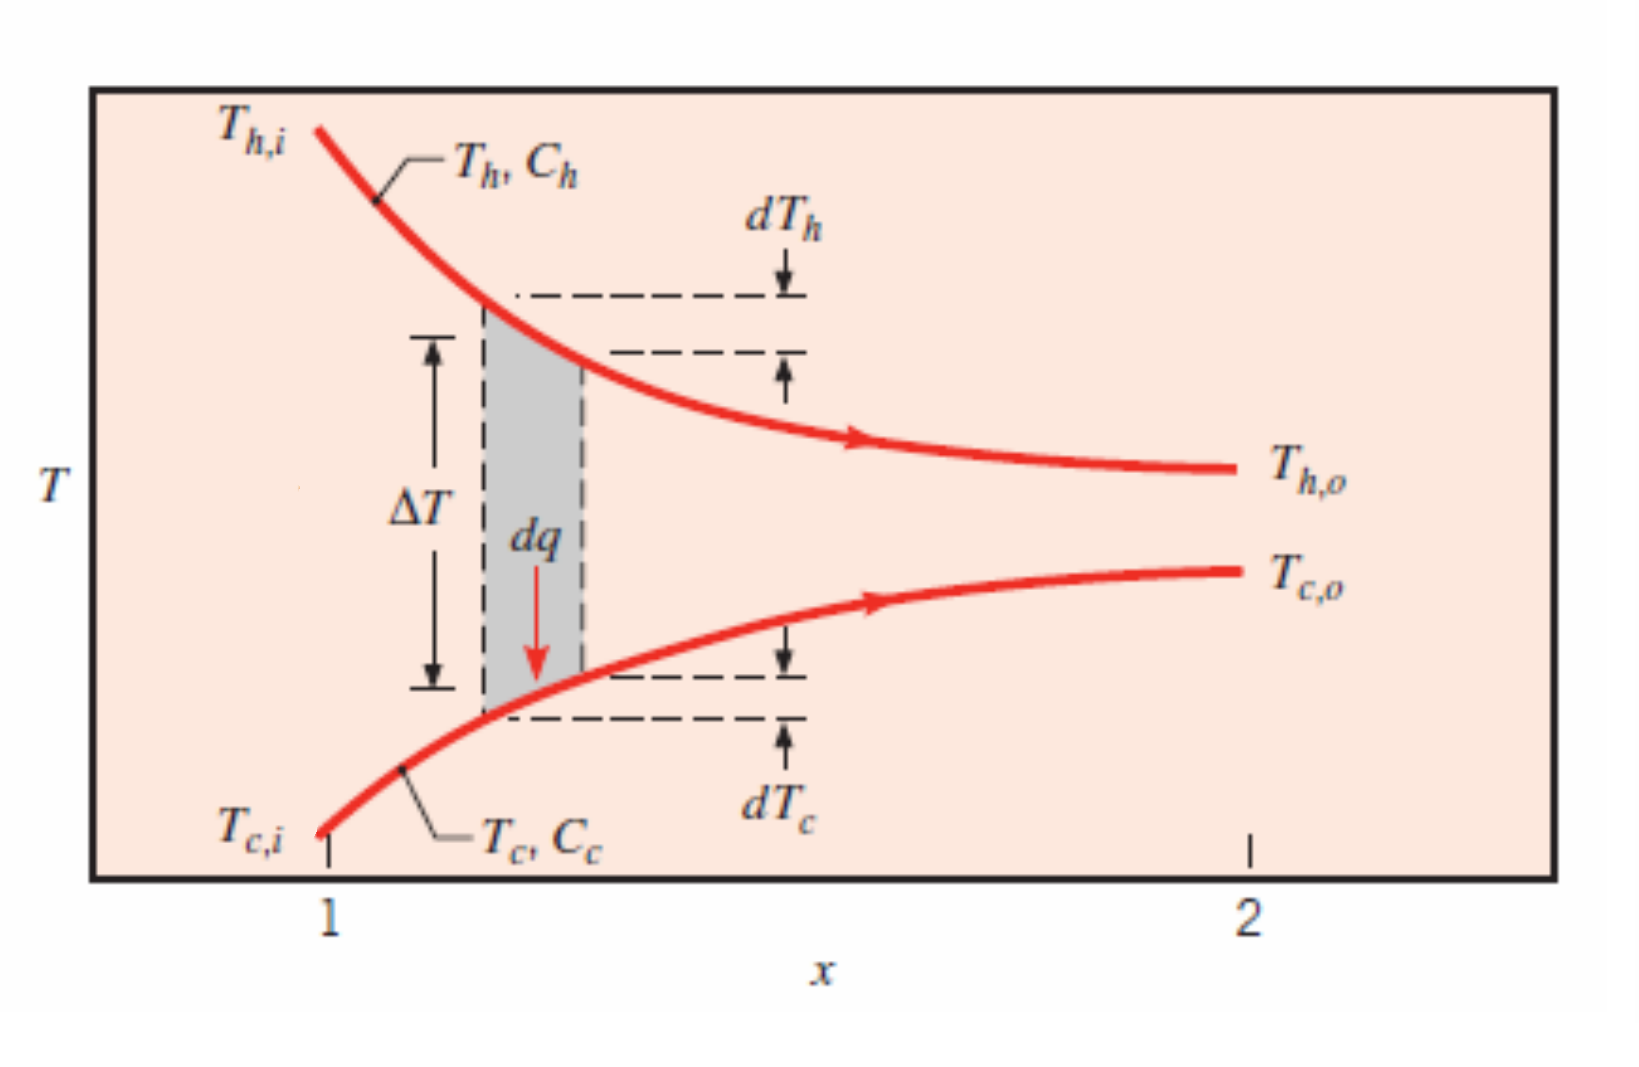
\includegraphics[width=\textwidth]{parallele_flow_T}
        \caption{Temperature profile for parallel flow HX \cite{Ngendakumana2018}.}
        \label{fig:C4_HX_par_flow_T}
    \end{subfigure}
    \begin{subfigure}[b]{0.45\textwidth}
        \centering
        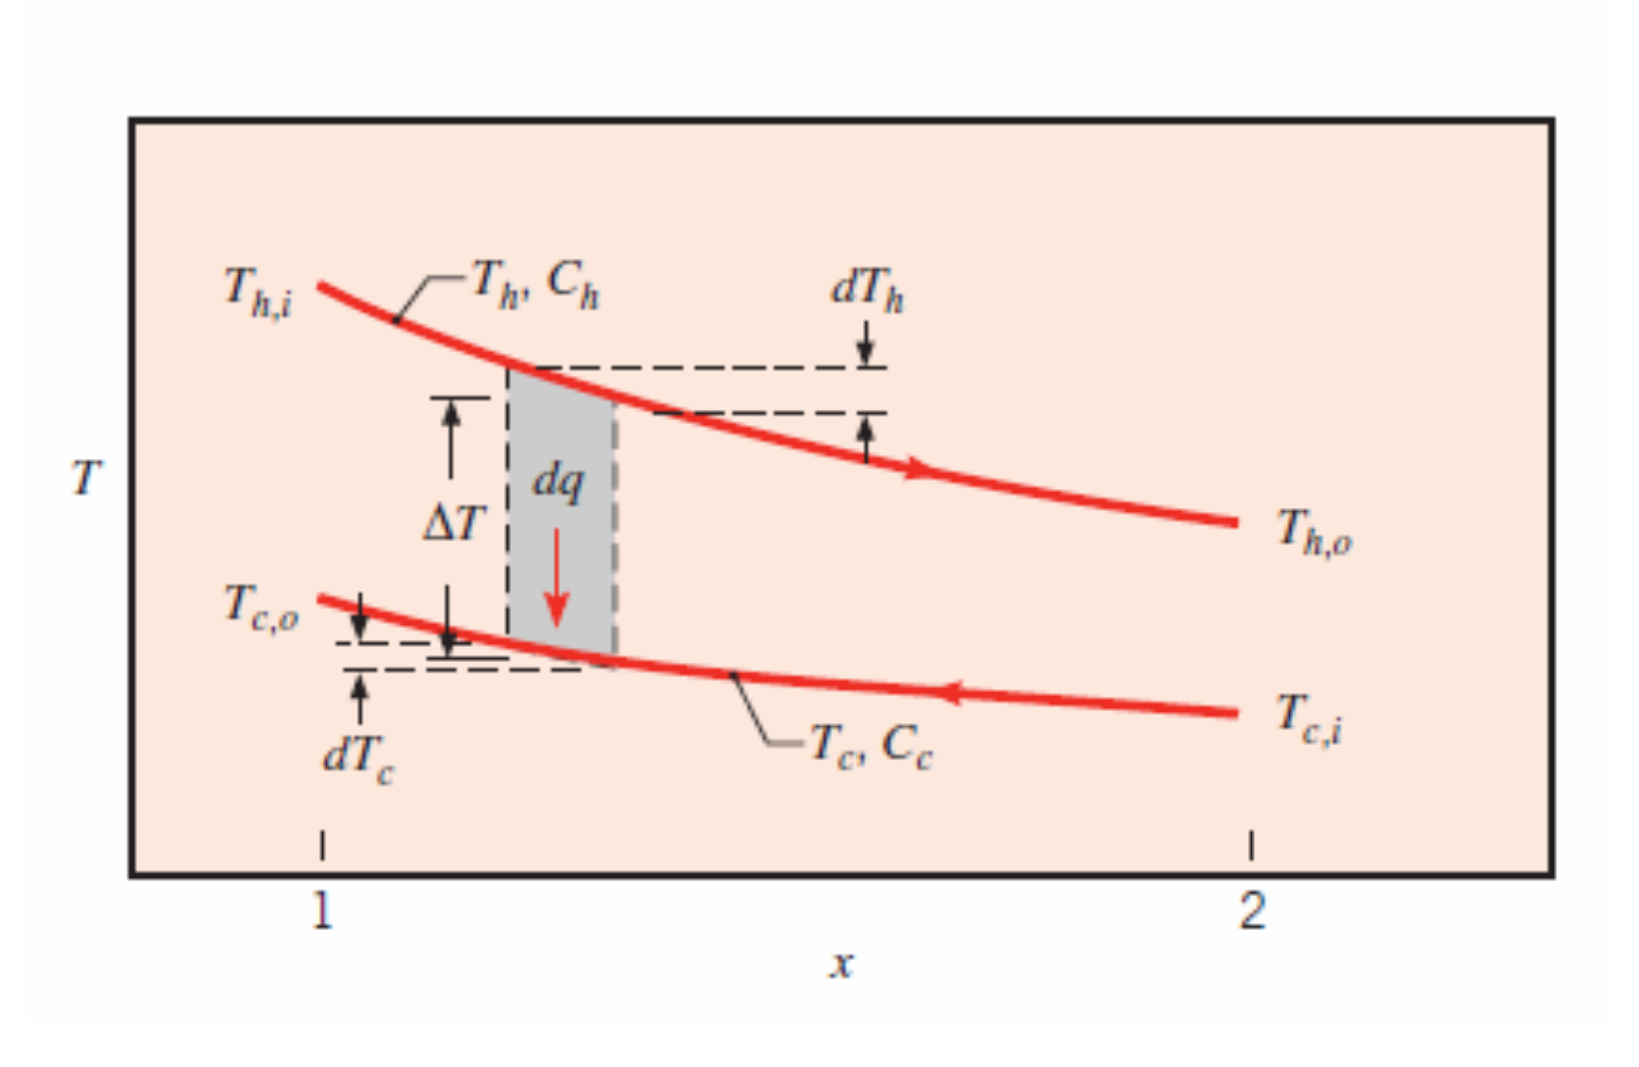
\includegraphics[width=\textwidth]{opposite_flow_T}
        \caption{Temperature profile for counter flow HX \cite{Ngendakumana2018}.}
        \label{fig:C4_HX_opo_flow_T}
    \end{subfigure}
    \caption{Temperature profiles for different stream configurations.}
    \label{fig:C4_Tprof}
\end{figure}

The subscripts $H$ and $C$ indicate which flow is considered (respectively the hot and the cold flow). The subscripts $i$ and $o$ refer to the inlet and the outlet of the heat exchanger.

The first temperature difference \(\Delta T_0\) is defined as being the largest temperature difference between the two flows, regardless of the position inside the HX. Thus, depending on the flow configuration, the \(\Delta T_0\) is given by (\ref{eq:C4_DT0}).

\begin{equation}
    \setstretch{1}
    \Delta T_0 =
    \begin{cases}
        T_{H,i} - T_{C,i} \text{ For the parallel flow} \\
        T_{H,i} - T_{C,o} \text{ For the counter flow}  \\
    \end{cases}\label{eq:C4_DT0}
\end{equation}

The second temperature difference \(\Delta T_L\) corresponds to the smallest temperature difference between the two flows. Similarly to \(\Delta T_0\), \(\Delta T_L\) is defined by the relation (\ref{eq:C4_DTL}).

\begin{equation}
    \setstretch{1}
    \Delta T_L =
    \begin{cases}
        T_{H,o} - T_{C,o} \text{ For the parallel flow} \\
        T_{H,o} - T_{C,i} \text{ For the counter flow}  \\
    \end{cases}\label{eq:C4_DTL}
\end{equation}

\subsection{Heat transfer within a heat exchanger}
\quad\ The heat transfer rate of a heat exchanger is directly dependent on the nature of the fluids and the heat exchanger itself. Let's consider the following relation (\ref{eq:C4_Qdot1})
\begin{equation}
    \dot{Q} = \frac{\Delta T_{LM}}{\mathrm{R}}= \mathrm{A}\cdot \mathrm{U}\cdot \Delta T_{LM}\label{eq:C4_Qdot1}
\end{equation}
Where \(\mathrm{A}\) is the global heat transfer area of the HX, and \(\mathrm{R}\) and \(\mathrm{U}\) are the global thermal resistance and heat transfer coefficient respectively. The difference of temperature \(\Delta T_{LM}\) is called the logarithmic mean temperature difference. Its definition is (\ref{eq:C4_lmtd}).


\begin{equation}
    \setstretch{1}
    \Delta T_{LM} = \frac{\Delta T_0-\Delta T_L}{ln\left(\frac{\Delta T_0}{\Delta T_L}\right)}\label{eq:C4_lmtd}
\end{equation}
With \(ln\) being the neperian logarithm.
\subsubsection{Transfer coefficient}
\quad\ The general definition of the product \(\mathrm{A}\cdot \mathrm{U}\) is written in the equation (\ref{eq:C4_AU}).
 
\begin{equation}
    \setstretch{1}
    \frac{1}{\mathrm{A}\cdot \mathrm{U}}  = \frac{1}{\eta_{0,C}\cdot h_{conv,C} \cdot A_C} + \frac{F_C}{\eta_{0,C}\cdot A_C} + R_w + \frac{F_H}{\eta_{0,H}\cdot A_H} + \frac{1}{\eta_{0,H}\cdot h_{conv,H} \cdot A_H}\label{eq:C4_AU}
\end{equation}
Where \(h_{conv}\) is the convective heat transfer coefficient (W/m$^2\cdot$K) of the fluid, \(F\) is a degradation factor due to the clogging, \(\eta_0\) is the global efficiency of the surface and \(R_w\) is the wall resistance.

Making the assumption that all the ducts considered in this work are smooth and the flows are turbulent, the convective heat transfer coefficient \(h_{conv}\) is obtained using the formula (\ref{eq:C4_h}).
\begin{equation}
    h_{conv} = Nu \cdot \frac{\lambda_c}{D_t} = 0.023\cdot Re^{0.8}\cdot Pr^{1/3}\frac{\lambda_C}{D_t}\label{eq:C4_h}
\end{equation}
Where \(Nu\), \(Re\) and \(Pr\) are respectively the Nusselt, Reynolds and Prandtl number. \(\lambda_c\) is the thermal conductivity (W/m$\cdot$K) of the fluid and \(D_t\) is the diameter of the duct\cite{Ngendakumana2018}.

By definition, the Reynolds and Prandtl numbers are defined as follows
\begin{align}
    Re & = \frac{\rho\cdot v\cdot D_h}{\mu}\label{eq:C4_Re} \\
    Pr & = \frac{\mu\cdot c_p}{\lambda_c}\label{eq:C4_Pr}
\end{align}
Where \(D_h\) is the hydraulic diameter, \(v\) is the velocity of the flow and \(\mu\) is the dynamic viscosity (Pa$\cdot$s). The hydraulic diameter and the flow velocity are respectively obtained using the two following relations (\ref
{eq:C4_Dh}) and (\ref{eq:C4_v}).

 \begin{align}
    D_h = \frac{4\cdot A_C}{P_C}\label{eq:C4_Dh}                      \\
    v=\frac{\dot{m}}{\rho\cdot\pi\cdot\frac{D_h^2}{4}}\label{eq:C4_v} \\
\end{align}
With \(A_c\) and \(P_c\) the cross area and perimeter of the duct\cite{Ngendakumana2018}.

Making the assumption that both \(D_h\) and \(D_t\) are equal, let's pose \(D=D_h=D_t\). Therefore, the convective heat transfer coefficient \(h_{conv}\) can be expressed as given in the relation (\ref{eq:C4_hconv}).


\begin{equation}
    \setstretch{1}
    h_{conv} = 0.0697\cdot \frac{\dot{m}^{4/5}\cdot c_p^{1/3}}{\pi^{4/5}\cdot D^{9/5}}\cdot \frac{\lambda_c^{2/3}}{\mu^{7/15}} \label{eq:C4_hconv}
\end{equation}

In the present work, the heat exchangers that will be used are plate heat exchangers with microchannel. The usage of ''microchannel systems allows the generation of local turbulence''\cite{Joseph2020}. These local turbulence enhance the heat transfer and thus, the efficiency of the heat exchanger.

Since the channel are really small, the assumption that the exchange surface dimensions \(\mathrm{A}\) for the cold and the hot side are equal will be made. Also, the wall resistance \(R_w\) will be neglected. This last assumption is acceptable when dealing with fluid for which the phase does not change during the heat transfer. For the gas turbine application, the fluid remains gaseous during all the process. 

\(\eta_0\) corresponds to the global efficiency of the heat exchanger fins \cite{GregoryNellis2015}. Since the global fin efficiency depends on the wall temperature, the fluid temperature and the geometry of the heat exchanger, it will be assumed that both sides of the heat exchanger are characterized by the same $\eta_0$. Therefore, the equality $\eta_{0_H}=\eta_{0,C}$ is enforced.

Finally, if the degradation factor $F$ is neglected, the heat transfer coefficient \(\mathrm{U}\) can be approached by the simple formulation (\ref{eq:C4_AU_prop}).


 \begin{equation}
    \setstretch{1}
    \mathrm{U} \simeq \frac{h_{conv,H}\cdot h_{conv,C}}{h_{conv,H} + h_{conv,C}}\label{eq:C4_AU_prop}
\end{equation}
\subsubsection{LMTD method}
\quad\ In the previous lines, a definition of the heat transfer rate based on the global transfer coefficient. This method is called the LMTD method and requires the knowledge of the geometry of the heat exchanger.
When the heat transfer rate \(\dot{Q}\) has been calculated, the temperatures at the outlet of the heat exchanger for the cold and hot stream can be computed using the two equations (\ref{eq:C4_ThQ}) and (\ref{eq:C4_TcQ}).

\begin{subequations}
    \setstretch{1}
    \begin{equation}
        \dot{Q} = \dot{m}_H\cdot c_{p,H}\cdot(T_{H,in} - T_{H,out}) =\dot{C}_H\cdot(T_{H,in} - T_{H,out}) \label{eq:C4_ThQ}
    \end{equation}
    \begin{equation}
        \dot{Q} = \dot{m}_C\cdot c_{p,C}\cdot (T_{C,out} - T_{C,in}) =\dot{C}_C\cdot (T_{C,out} - T_{C,in}) \label{eq:C4_TcQ}
    \end{equation}
\end{subequations}
Where $\dot{C}$ corresponds to the heat capacity rate (W/K).
This method requires the knowledge of the inlet and outlet temperatures of both fluids before initiating the computation of the heat transfer rate \(\dot{Q}\) using the relation (\ref{eq:C4_Qdot1}). Therefore, this method needs iterations in the event where these temperatures are not known a priori.

\subsubsection{$\varepsilon$-NTU method}
\quad\ There exists a second method for the evaluation of the heat transfer rate which does not need the outlet temperature of the fluids. First, the maximum heat transfer rate \(\dot{Q}_{max}\) is computed base the formula (\ref{eq:C4_Qmax}).


\begin{align}
    \setstretch{1}
    \dot{Q}_{max} = \dot{C}_{min}\cdot (T_{h,in} - T_{c,in})\label{eq:C4_Qmax}\\
    \text{with }\dot{C}_{min}=min(\dot{C}_H,\dot{C}_C)\nonumber
\end{align}


Then, the actual heat transfer rate $\dot{Q}$ is obtained by multiplying the maximum heat transfer rate by the efficiency of the heat exchanger.


\begin{equation}
    \setstretch{1}
    \dot{Q} = \varepsilon\cdot\dot{Q}_{max} \label{eq:C4_Qdot}
\end{equation}
Where \(\varepsilon\) is the efficiency of the heat exchanger. This efficiency is a function of the ratio \(C_r = \frac{\dot{C}_{min}}{\dot{C}_{max}}\), the flow arrangement, and the number of transfer unit NTU defined as stated in the relation (\ref{eq:C4_NTU})


\begin{equation}
    \setstretch{1}
    \text{NTU} = \frac{\mathrm{A}\cdot \mathrm{U}}{\dot{C}_{min}}\label{eq:C4_NTU}
\end{equation}

It can be noticed that the definition of the NTU involves the global exchange area $\mathrm{A}$ and the global heat transfer coefficient $\mathrm{U}$. This implies that both the NTU and the efficiency $\varepsilon$ depend on the flow configuration and geometry of the heat exchanger .  

Here, the type of heat exchanger used for the modeled Brayton cycle is plate heat exchanger with microchannel. Since the flow configuration for this type of heat exchanger is counter flow, the associated relation linking the efficiency \(\varepsilon\) to the number of transfer units  NTU is
\begin{equation*}
    \varepsilon = \frac{1 - e^{-NTU\cdot \left(1 - C_r\right)}}{1 - C_r\cdot e{-NTU\cdot \left(1 - C_r\right)}}\cite{GregoryNellis2015}
\end{equation*}
%%%%%%%%%%%%%%%
%ECRIRE ANNEXE%
%%%%%%%%%%%%%%%

Once the coefficient \(\varepsilon\) computed, the outlet temperatures of the fluids can be obtained using the relations (\ref{eq:C4_ThQ}) and (\ref{eq:C4_TcQ}).


\section{Piping and pressure drop}
%%%%%%%%%%%%%%%%%%%%%%%%%%%%%%%%%%%
%%%%%                         %%%%%
%%%%%       <<Piping>>        %%%%%
%%%%%                         %%%%%
%%%%%%%%%%%%%%%%%%%%%%%%%%%%%%%%%%%
\quad\ From now, the loss of pressure inside the different elements has not been considered. However, for a system like a gas turbine, the pressure drops have to be as minimal as possible to guarantee that the expanded gas in the turbine is at a pressure as high as possible.

In this work, simple formula will be applied for the pressure drops computation. The pressure drops are computed based on a pressure drop factor \(Dp\) varying from 0 to 1. Then the pressure at the outlet of the component is given by the relation (\ref{eq:C4_Pdrop}).

\begin{equation}
    \setstretch{1}
    p_{o} = p_{i}\cdot (1 - Dp)\label{eq:C4_Pdrop}
\end{equation}
Where the factor \(Dp\) is different for each component of the system. Indeed, the probability that the pressure drop through a combustion chamber and a heat exchanger are equal are really small.

It can be demonstrated that the pressure difference \(\Delta p = p_{i} - p_{o}\) is a quadratic function of the mass flow rate \(\dot{m}\). The simplest way to define the pressure drop is to measure difference for a nominal point of operation. Then, using the relation (\ref{eq:C4_DP}) allows computing the pressure drop for any non-nominal conditions.

\begin{equation}
    \setstretch{1}
    \Delta p \simeq \Delta p_{nom}\cdot \frac{\dot{m}^2}{\dot{m}^2_{nom}}\label{eq:C4_DP}
\end{equation}

\newpage
%%%%%%%%%%%%%%%%%%%%%%%%%%%%%%%%%
%% Chapitre 5:                 %%
%% Brayton_cycle               %%
%%%%%%%%%%%%%%%%%%%%%%%%%%%%%%%%%
\graphicspath{{Chapitre_5/Images/}}
\chapter{Brayton cycle}\label{C5}
%%%%%%%%%%%%%%%%%%%%%%%%%%%%%%%%%%%
%%%%%                         %%%%%
%%%%% Brayton cycle chapitre 5 %%%%%
%%%%%                         %%%%%
%%%%%%%%%%%%%%%%%%%%%%%%%%%%%%%%%%%
\quad\, In the introduction, the simplest configuration for the Brayton gas cycle has been defined as being a cycle successively composed of a compressor, a combustion chamber and a turbine. This simple configuration is called Gas Turbine or GT. 

The previous chapter \ref{C4} described individually these components by providing the required theoretical notions to be able to analyze their performances. Now, the components will be considered together as a thermodynamic cycle to assess the performances of the Gas Turbine and of its existing variants.

\section{Gas Turbine}
%%%%%%%%%%%%%%%%%%%%%%%%%%%%%%%%%%%
%%%%%                         %%%%%
%%%%%     <<Gas Turbine>>     %%%%%
%%%%%                         %%%%%
%%%%%%%%%%%%%%%%%%%%%%%%%%%%%%%%%%%
\quad\, The Gas Turbine (GT) is the most basic configuration of the Brayton cycle. As it is illustrated in the Figure \ref{fig:C5_BraytonGT}, the three main components are the compressor (COMP), the combustion chamber (CC) and the turbine (TURB).

\begin{figure}[h]
\centering
\includegraphics[scale=0.15] {GT}
\caption{Gas Turbine (GT)}
\label{fig:C5_BraytonGT}
\end{figure}

The compressor and the turbine are both installed on the same shaft. Since there aren't any gearbox, the rotational speed of both turbomachines is the same. The generator (G) is also attached to the shaft to convert the generated mechanical power into electricity. 
When the machine starts, the generator becomes a motor to provide the required energy to help the turbine. Indeed, at low rotational speed the power consumed by the compressor is usually greater than the power produced by the turbine alone. 



As it is illustrated in the Figure \ref{fig:C5_BraytonGT}, the cycle can be decomposed into eight thermodynamic states. For each connection between two elements, there are piping that will induce some pressure drops. For each of these states, the temperature and pressure are measured in order to fully characterized the state. The Table \ref{tab:C5_thermo_state_GT} includes the different states emphasized on Figure \ref{fig:C5_BraytonGT}.
\begin{longtable}[c]{@{}lcc@{}}
\caption{Thermodynamic states - gas cycle (GT)}
\label{tab:C5_thermo_state_GT}\\
\toprule
\textbf{State n\degree} & $\mathbf{T}$      & $\mathbf{p}$      \\* \midrule
\endfirsthead
%
\endhead
%
\bottomrule
\endfoot
%
\endlastfoot
%
\textbf{0}              & $T_0$ = $T_{ref}$ & $p_0$ = $p_{ref}$ \\
\textbf{1}              & $T_1$ = $T_{amb}$ & $p_1$ = $p_{amb}$ \\
\textbf{2}              & $T^0_2=T_1$       & $p^0_2\leq p_1$   \\
\textbf{3}              & $T^0_3>T^0_2$     & $p^0_3>p^0_2$     \\
\textbf{4}              & $T_4=T^0_3$       & $p_4\leq p^0_3$   \\
\textbf{5}              & $T_5>>T_4$        & $p_5\leq p_4$     \\
\textbf{6}              & $T^0_6=T_5$       & $p^0_6\leq p_5$   \\
\textbf{7}              & $T^0_7<T^0_6$     & $p^0_7<p^0_6$     \\
\textbf{8}              & $T_8=T^0_7$       & $p_8=p_1<p^0_7$   \\* \bottomrule
\end{longtable} 
Where the state \textbf{0} corresponds to the reference conditions. It is worth noting that for the compressor and the turbine, the stagnation quantities are used. The reason is that in this work, method to compute the Mach number hasn't been considered. This is the reason why the pressure ratios and the isentropic efficiency that will be considered for the compressor and the turbine are based on total quantities.

For each of the mentioned states, five thermodynamic properties are evaluated. Namely the temperature, pressure, enthalpy, entropy and density. For the last variable, the ideal gas equation (\ref{eq:C2_GP}) from the chapter \ref{C2} is used. 

A graphical representation of these states can be performed by drawing some thermodynamic diagrams. Here, the p-v and T-s diagrams have been drawn in the Figures \ref{fig:C5_pv_GT} and \ref{fig:C5_Ts_GT} respectively. 

The choice of the T-s diagram instead of the h-s diagram is motivated by the fact that temperatures are quantities that have an easier interpretation. Since only ideal gases are considered, the enthalpy variation is equivalent to the temperature variation multiplied by the heat capacity at constant pressure.

The diagrams have been obtained using the computer code that will be described in the next chapters. For now, let's just assume that the program is just a black box.


\begin{figure}[H]
     \centering
     \begin{subfigure}[b]{0.4\textwidth}
         \centering
         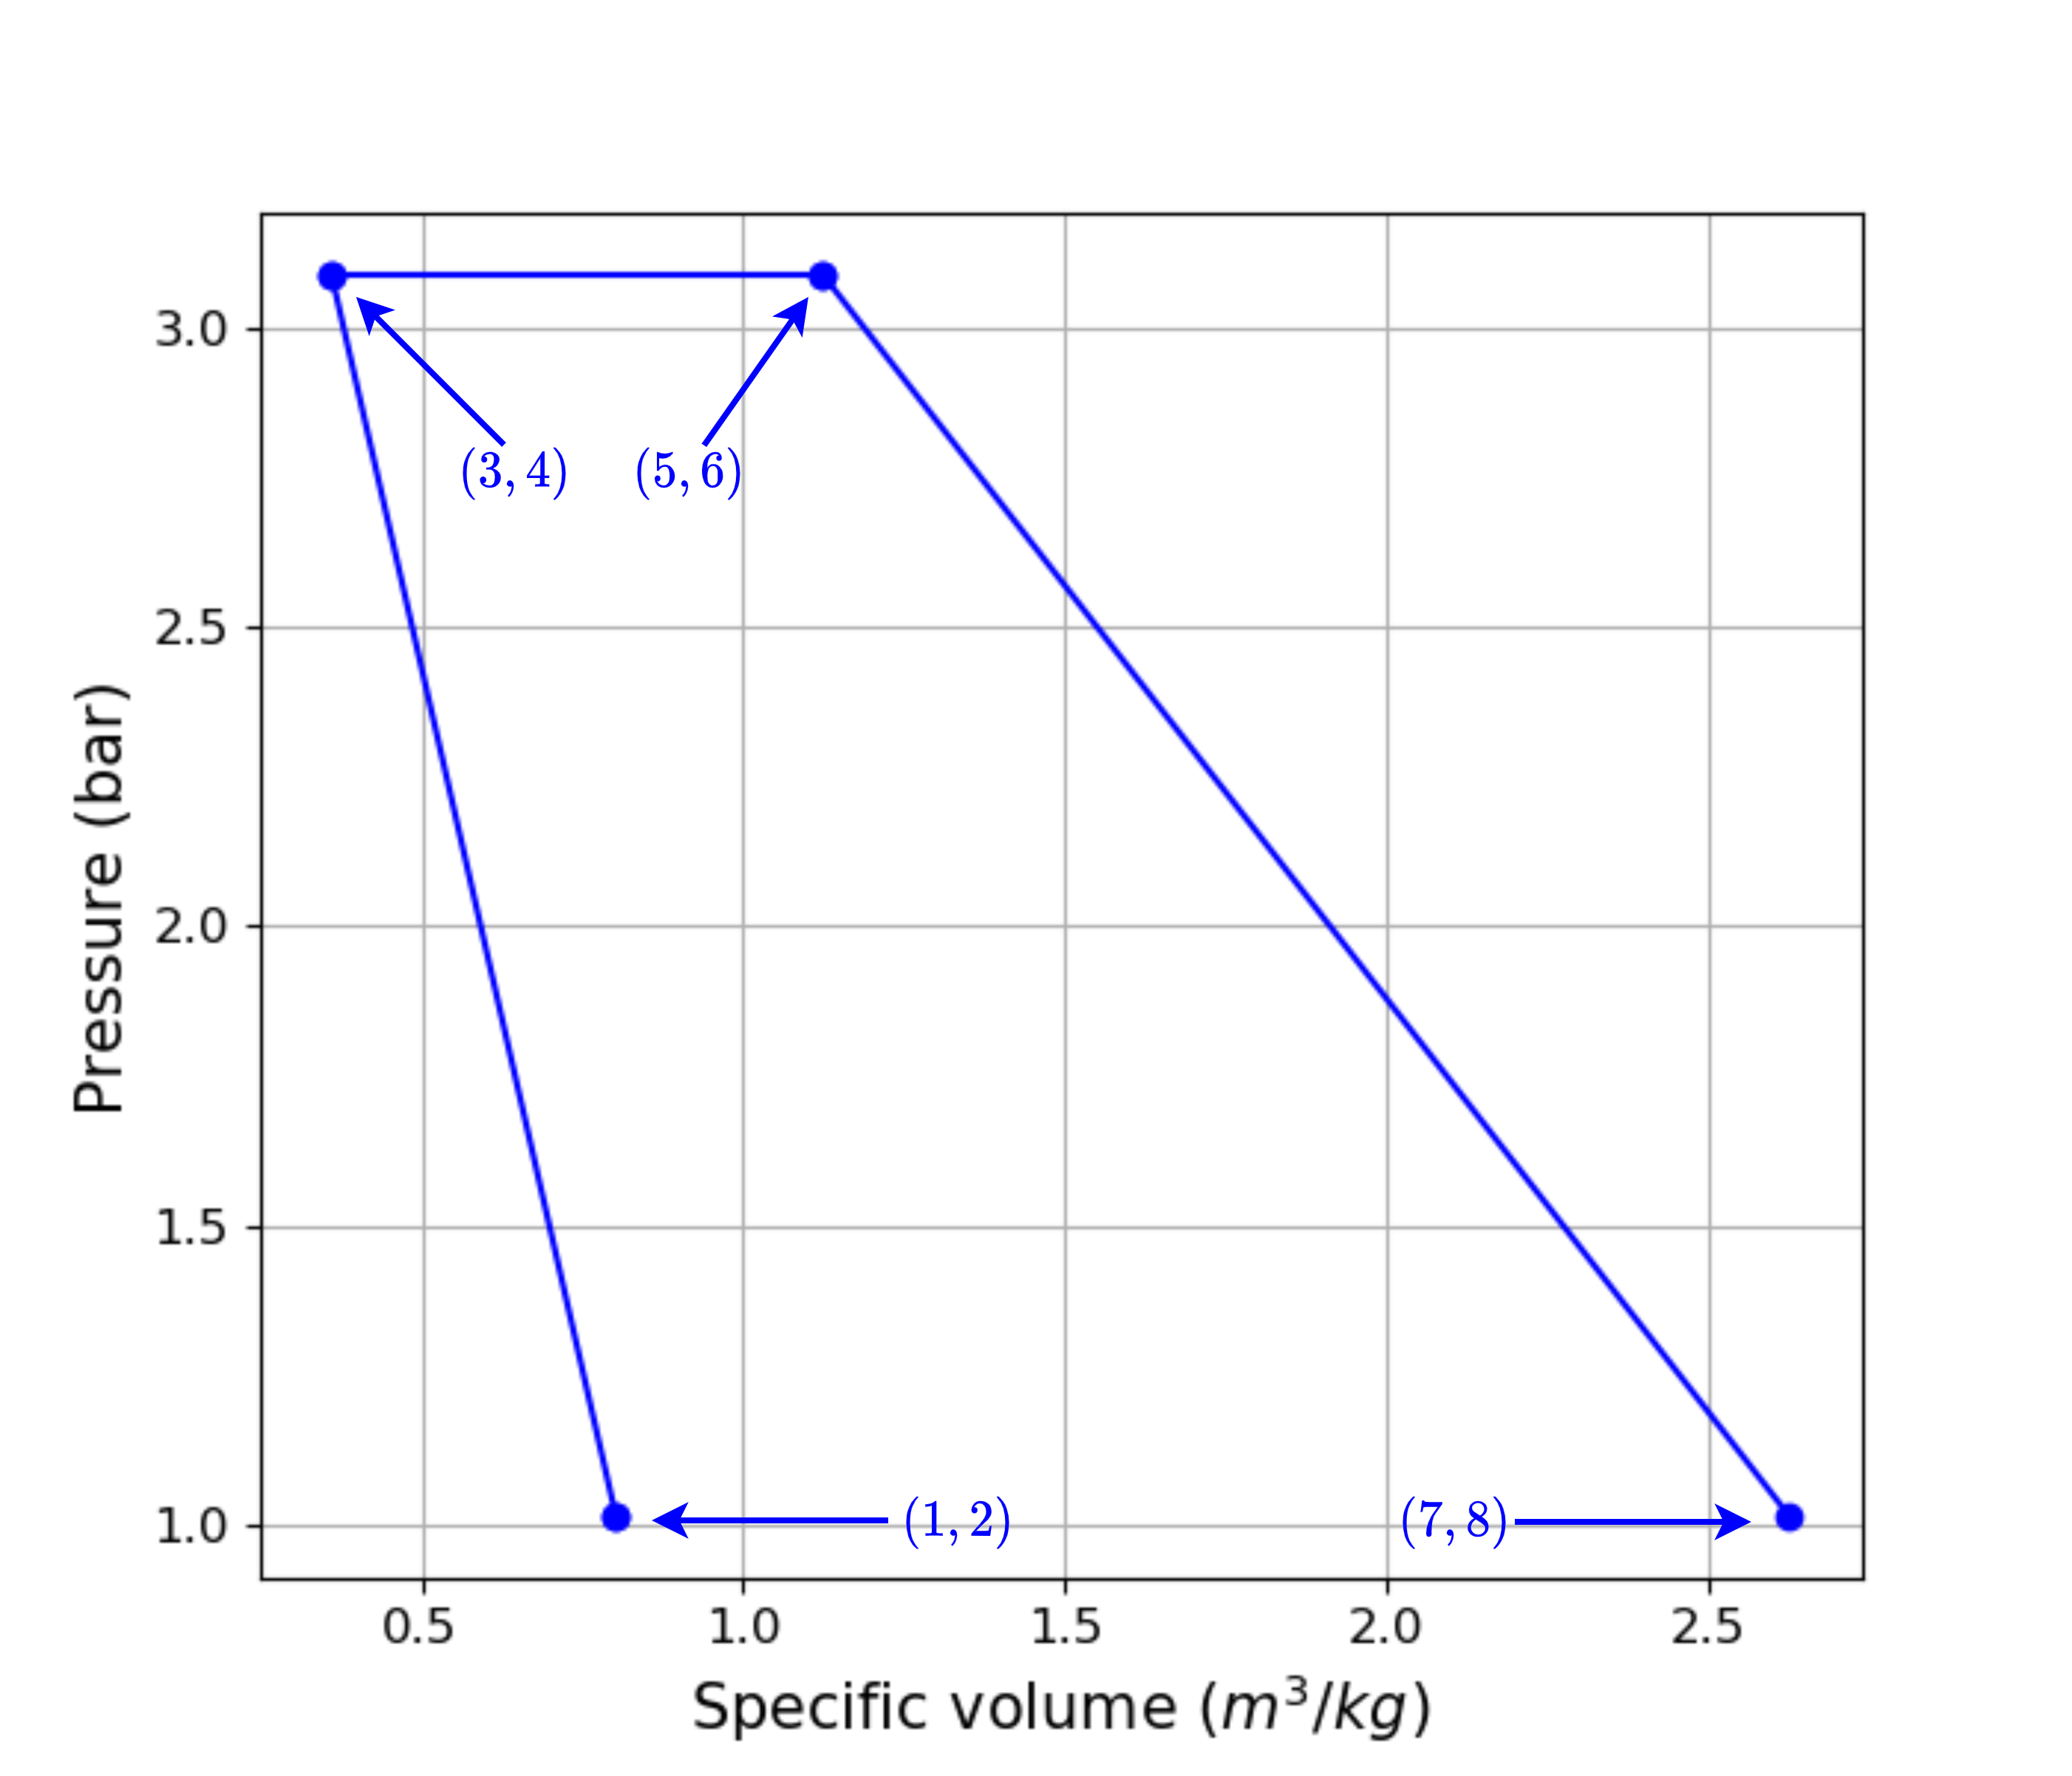
\includegraphics[width=\textwidth]{pv_GT}
         \caption{p-v diagram}
         \label{fig:C5_pv_GT}
     \end{subfigure}
     \begin{subfigure}[b]{0.4\textwidth}
         \centering
         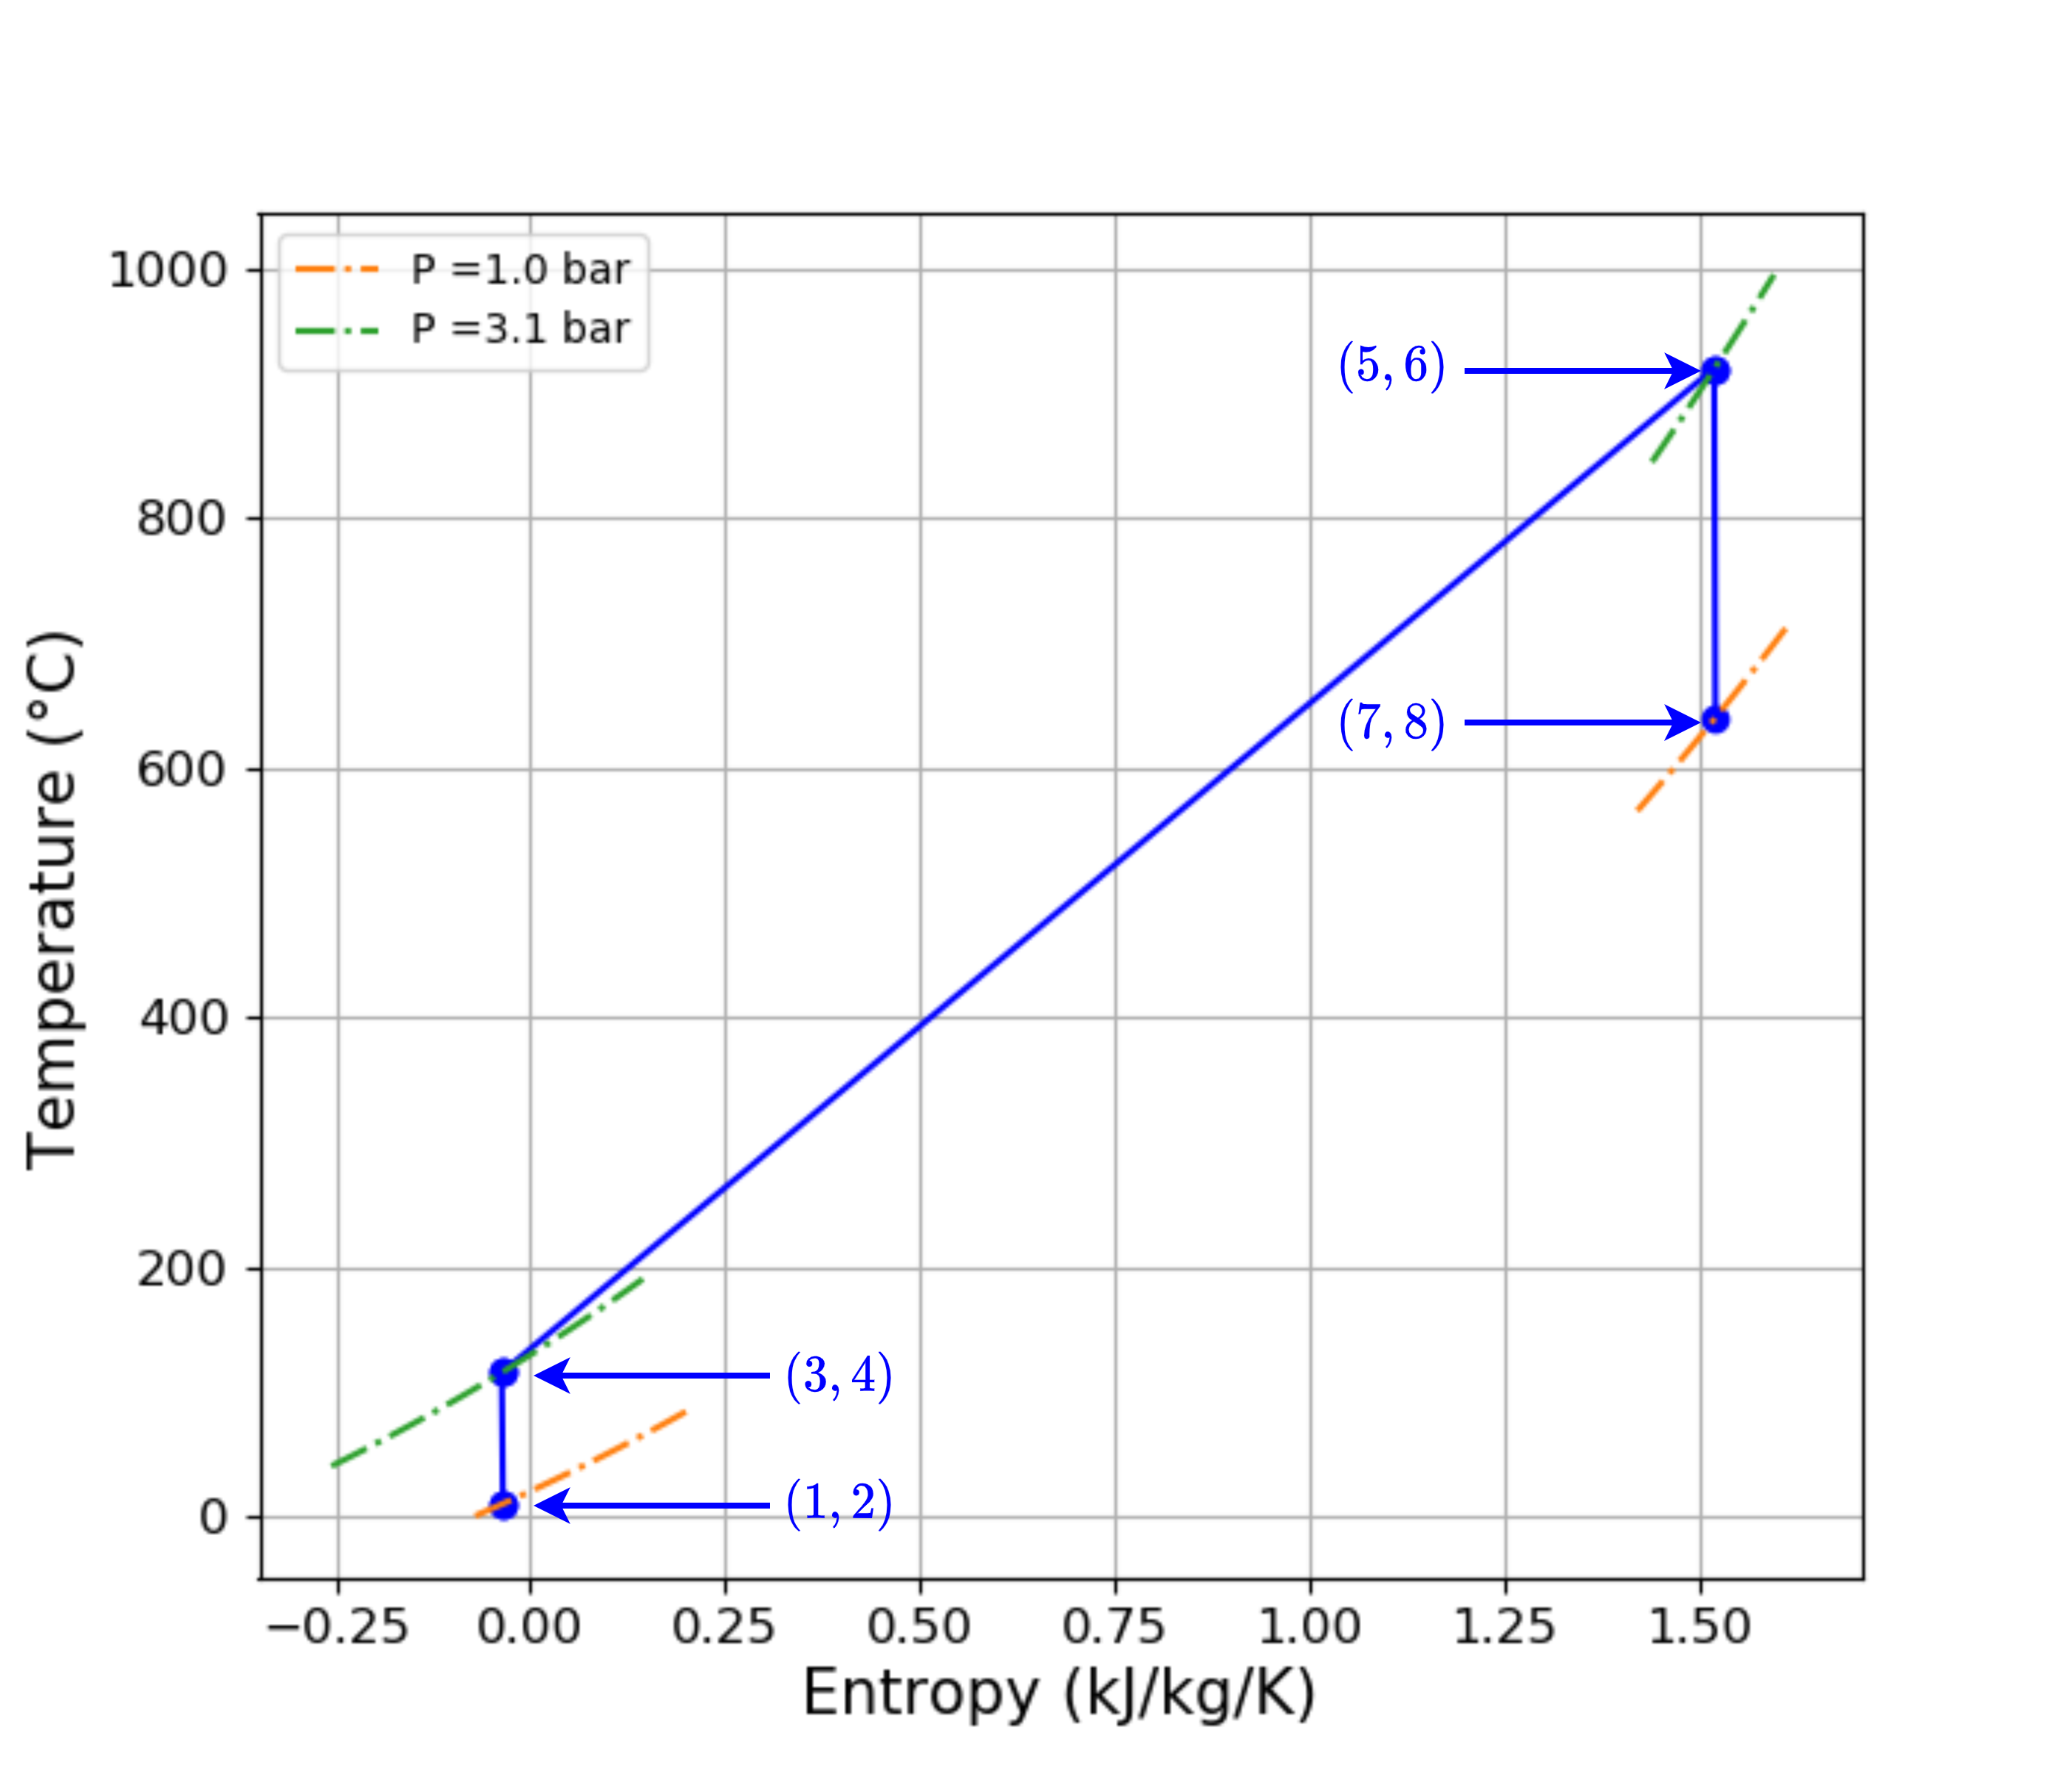
\includegraphics[width=\textwidth]{Ts_GT}
         \caption{T-s diagram}
         \label{fig:C5_Ts_GT}
     \end{subfigure}
        \caption{Thermodynamic diagrams - Gas Turbine}
        \label{fig:C5_thermo_diagram_GT}
\end{figure}

These two diagrams have been obtained considering ideal components. An ideal component is characterized by the efficiency of 100\%. This means that there aren't any pressure drops, the isentropic efficiency $\eta_{is}$ of the compressor and the turbine is equal to 100\%, and the combustion chamber efficiency $\eta_{cc}$ is also equal to 100\%.

As it can be noticed, the graphs are open. Indeed, the exhaust gas from the outlet of the turbine is returned to the environment with all its energy. The transformation from the state \textbf{8} to the state \textbf{1} would correspond to the return at the ambient conditions of the exhaust gas. 

The net work provided by the Brayton cycle corresponds to the area inscribed in the loop \textbf{1}$\rightarrow$\textbf{8}$\rightarrow$\textbf{1}. Mathematically, it is obtained by computing one of the two integrals (\ref{eq:C5_W}) and (\ref{eq:C5_Ws}). These two integrals are respectively associated to the p-v and T-s diagrams.

\begin{subequations}  
\setstretch{1}
\begin{align}
    W_{net} = \oint_{cycle}pdv\label{eq:C5_W}\\
    W_{net} = \oint_{cycle}Tds\label{eq:C5_Ws}
\end{align}
\end{subequations}

Now considering the T-s diagram, it shows the effect of the isentropic efficiency regarding to the evolution of the entropy during the compression and the expansion. Here, since the isentropic efficiency have been set to 100\%, the entropy at the beginning and the end of these transformations are equal. If real components were considered, the entropy would increase during the compression and the expansion.

In the T-s diagram are also represented the iso-pressure lines. Both the compressor and the turbine operate between 1 bar and 3.1 bars. It can be  proved that the thermal efficiency of the ideal GT cycle is proportional to the pressure ratio across the compressor. 

The thermal efficiency of any Brayton cycle is defined as being the ratio (\ref{eq:C5_etath}) between the net power output $\dot{W}_{net}$ and the heat transfer rate from coming from the injected fuel.

\begin{equation}
    \setstretch{1}
    \eta_{th} = \frac{\dot{W}_{net}}{\dot{m}_{fuel}\cdot HCV_{fuel}} \label{eq:C5_etath}
\end{equation}
Where $HCV_{fuel}$ is the low heat calorific value (J/kg) of the fuel.

Considering the presented ideal GT cycle, the thermal efficiency $\eta_{th,GT} =24$\%, and the net power output of the cycle is equal to 42.05 kW. The net power output is defined as being the power $\dot{W}_t$ produced by the turbine minus the power $\dot{W}_c$ consumed by the compressor.

To compute these two powers, it is required to calculate the work involved during the expansion and the compression. Both can be obtained by computing the variation of the total enthalpy between the inlet and the outlet of the two turbomachines (relations (\ref{eq:C5_Wt}) and (\ref{eq:C5_Wc})) (respectively).

\begin{subequations}
\setstretch{1}
\begin{align}
    W_t = h^0_6 - h^0_7 = c_p\cdot(T^0_6 - T^0_7)\label{eq:C5_Wt}\\
    W_c = h^0_2 - h^0_3 = c_p\cdot(T^0_2 - T^0_3)\label{eq:C5_Wc}
\end{align}
\end{subequations}
Then, the powers $\dot{W}_t$ and $\dot{W}_c$ are obtained by multiplying the works by the mass flow rate going through each turbomachine. Due to the injection of fuel $\dot{m}_{fuel}$ between the compressor and the turbine, the mass flow rate of gas $\dot{m}_{gas}=\dot{m}_{air}+\dot{m}_{fuel}$ in the turbine is higher than the mass flow rate of air $\dot{m}_{air}$ .


It can be noticed that at the exhaust of the cycle, the thermal energy available within the gas is still non-negligible. This energy at high temperature has a great potential and could be utilized to improve the cycle and its thermal efficiency. A possible way of improvement will be given in the following section.\newpage

\section{Regenerative Gas Turbine}
%%%%%%%%%%%%%%%%%%%%%%%%%%%%%%%%%%%
%%%%%                         %%%%%
%%%%%    <<regenerative>>     %%%%% 
%%%%%     <<Gas Turbine>>     %%%%%
%%%%%                         %%%%%
%%%%%%%%%%%%%%%%%%%%%%%%%%%%%%%%%%%
\quad\, As seen in the previous section, the gas cycle does not have a really high efficiency. This is due to the huge amount of energy available in the exhaust gas that is wasted. However, this high-level energy could be used to preheat the air before entering the combustion chamber. 

This is done by using a heat exchanger called regenerator. By adding a regenerator, the amount of energy to be provided to the combustion chamber to reach the same target temperature will be smaller since the inlet temperature of the air will be higher.

This variant of the Gas Turbine cycle is called Regenerative Gas Turbine (RGT) cycle. A schematic of this cycle is given in the Figure \ref{fig:C5_RGT}.

\begin{figure}[h]
\centering
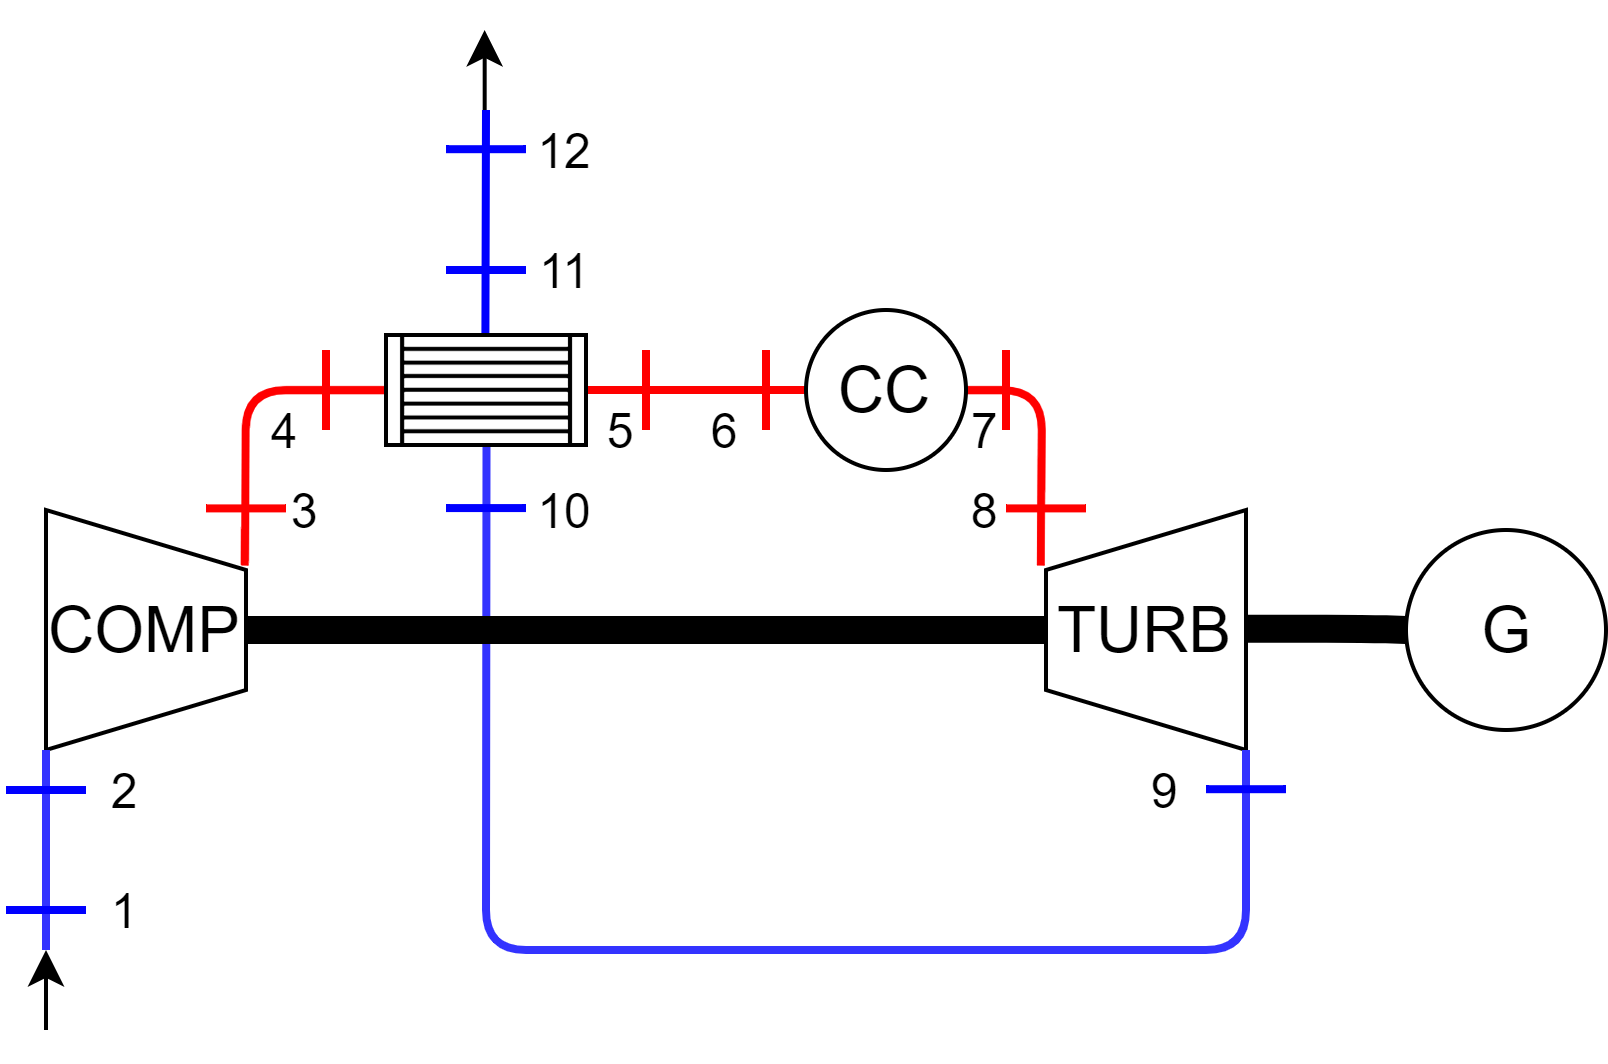
\includegraphics[scale=0.15]{RGT}
\caption{Regenerative GT (RGT)}
\label{fig:C5_RGT}
\end{figure}

Similarly to the GT cycle, to maximum thermal efficiency $\eta_{is,RGT}$ of the cycle is achieved by considering all the components as ideal. In addition to the turbomachines and the combustion chamber, the efficiency of the heat exchanger will be set at 100\%. 

The states from \textbf{1} to \textbf{12} can be represented by the p-v and T-s  diagrams. The two diagrams are included in the set of Figures \ref{fig:C5_thermo_diagram_RGT}.

\begin{figure}[h]
     \centering
     \begin{subfigure}[b]{0.4\textwidth}
         \centering
         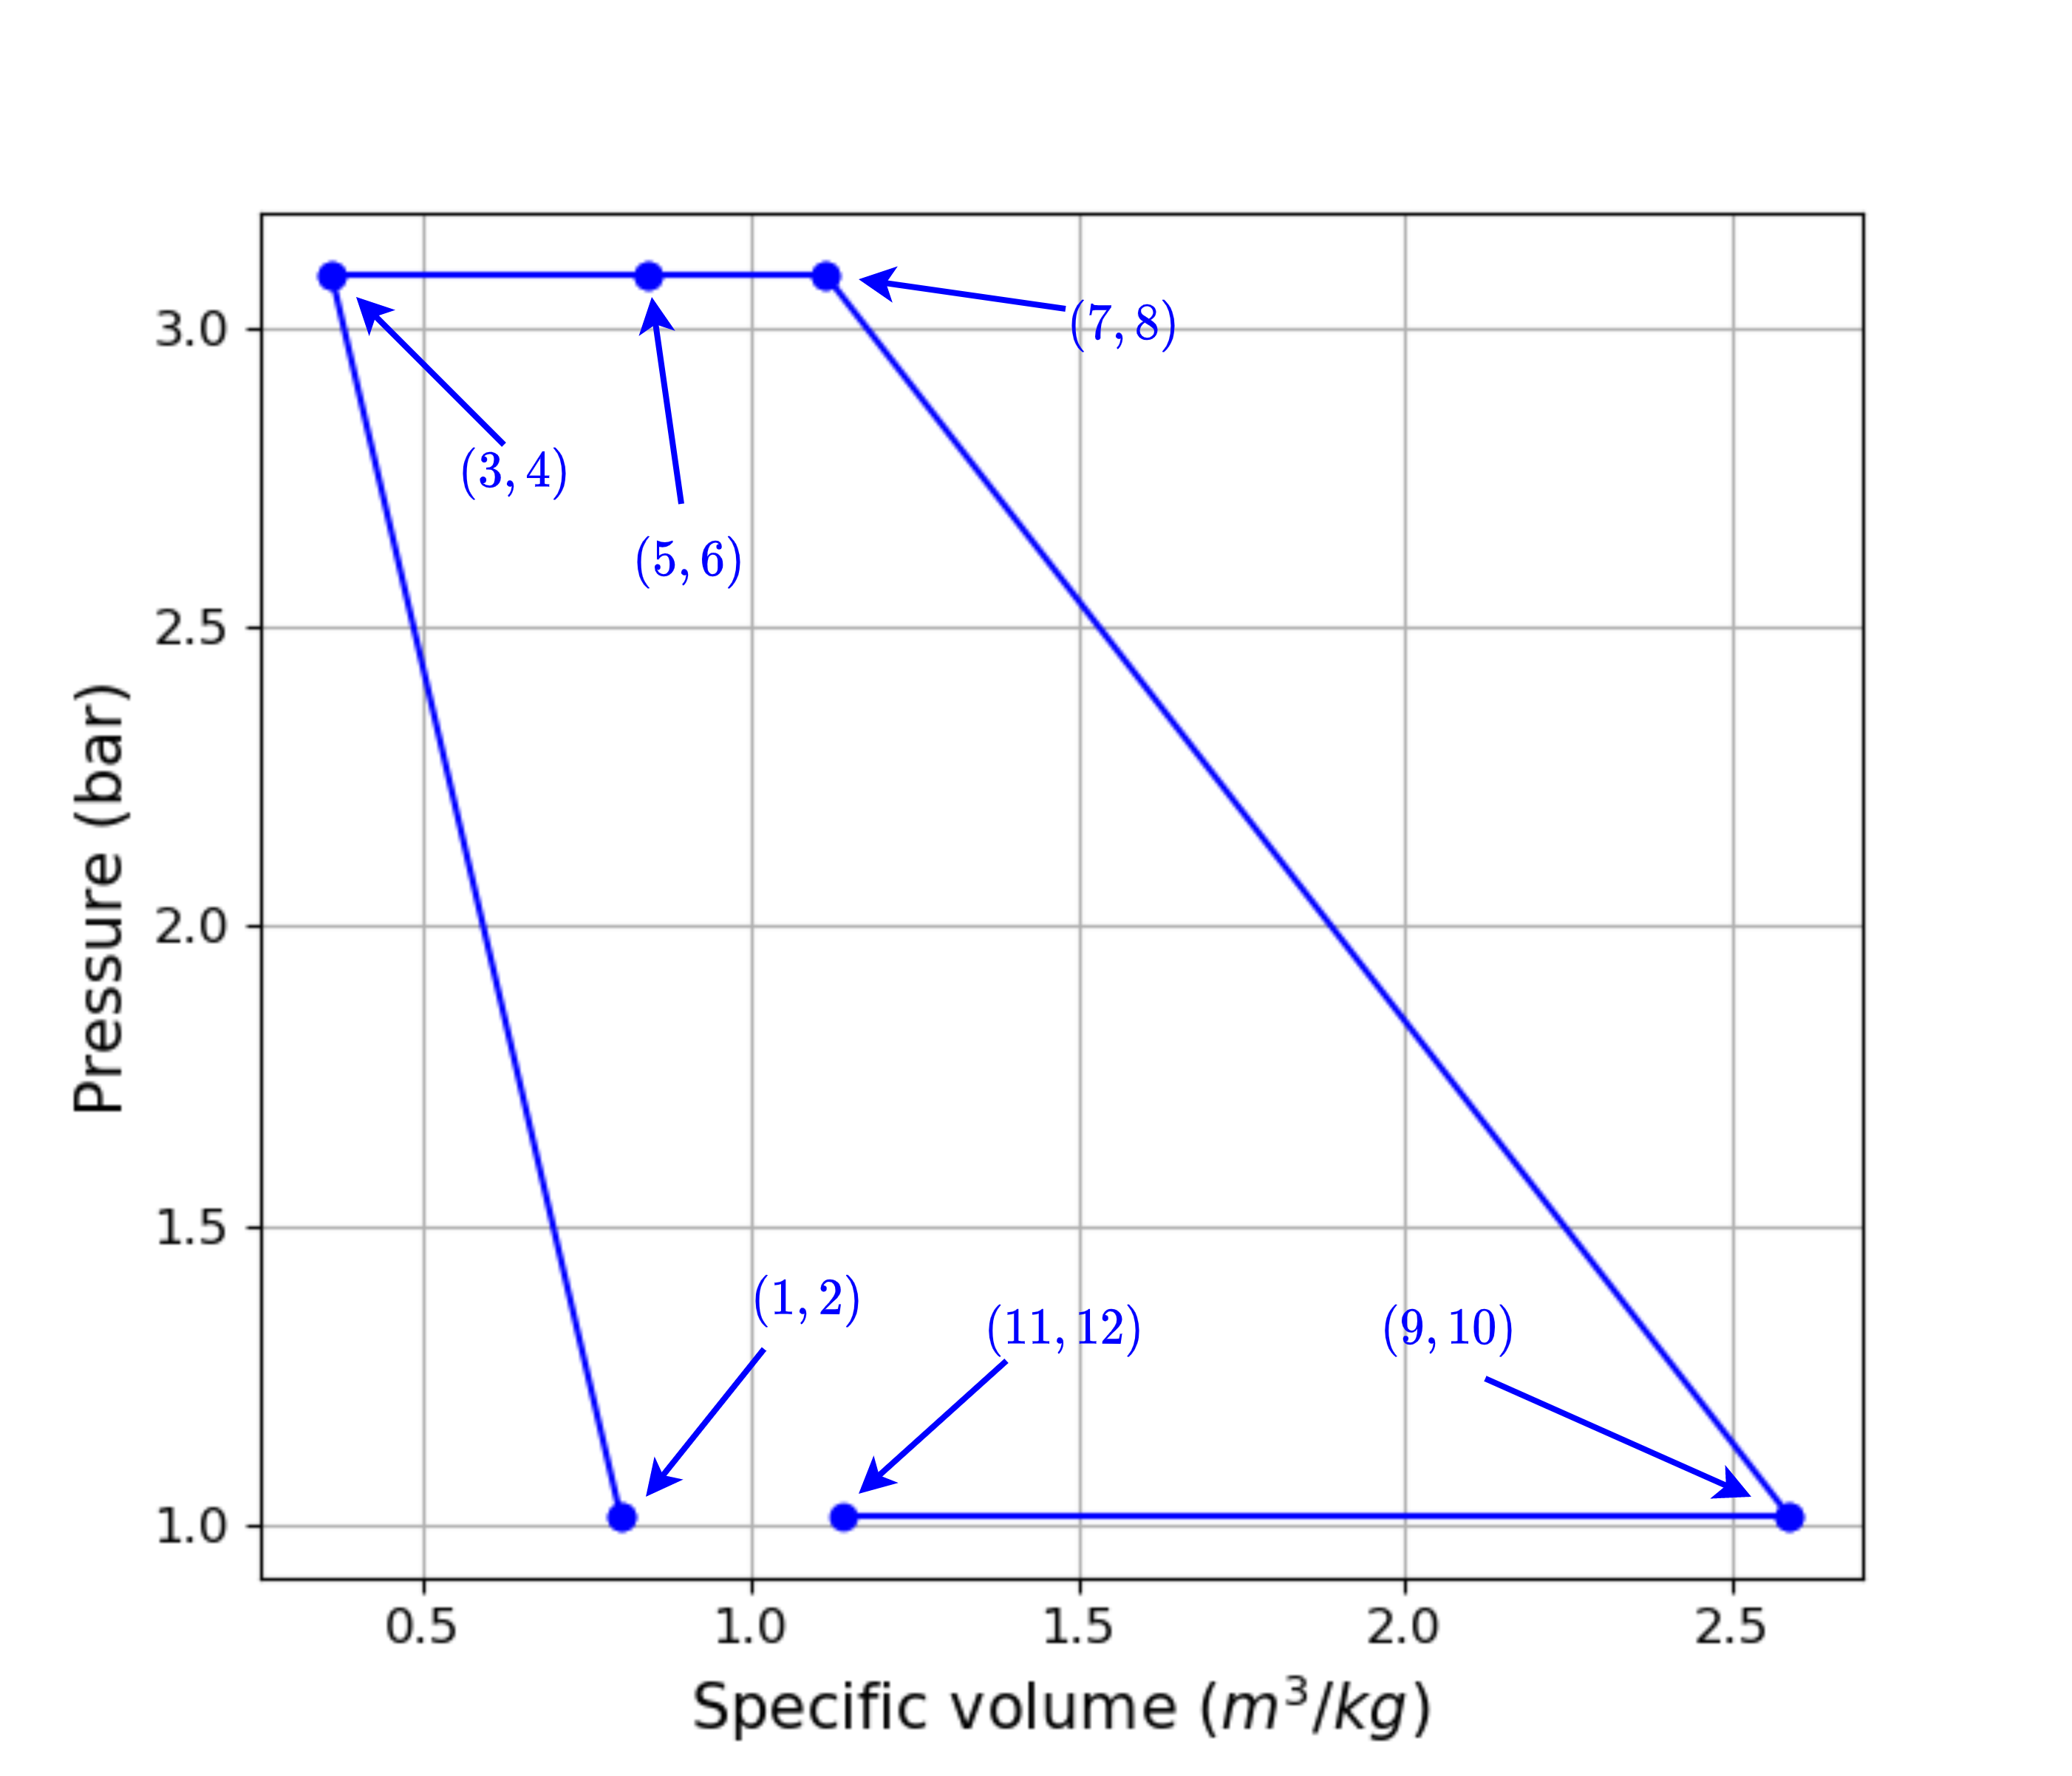
\includegraphics[width=\textwidth]{pv_RGT}
         \caption{p-v diagram}
         \label{fig:C5_pv_RGT}
     \end{subfigure}
     \begin{subfigure}[b]{0.4\textwidth}
         \centering
         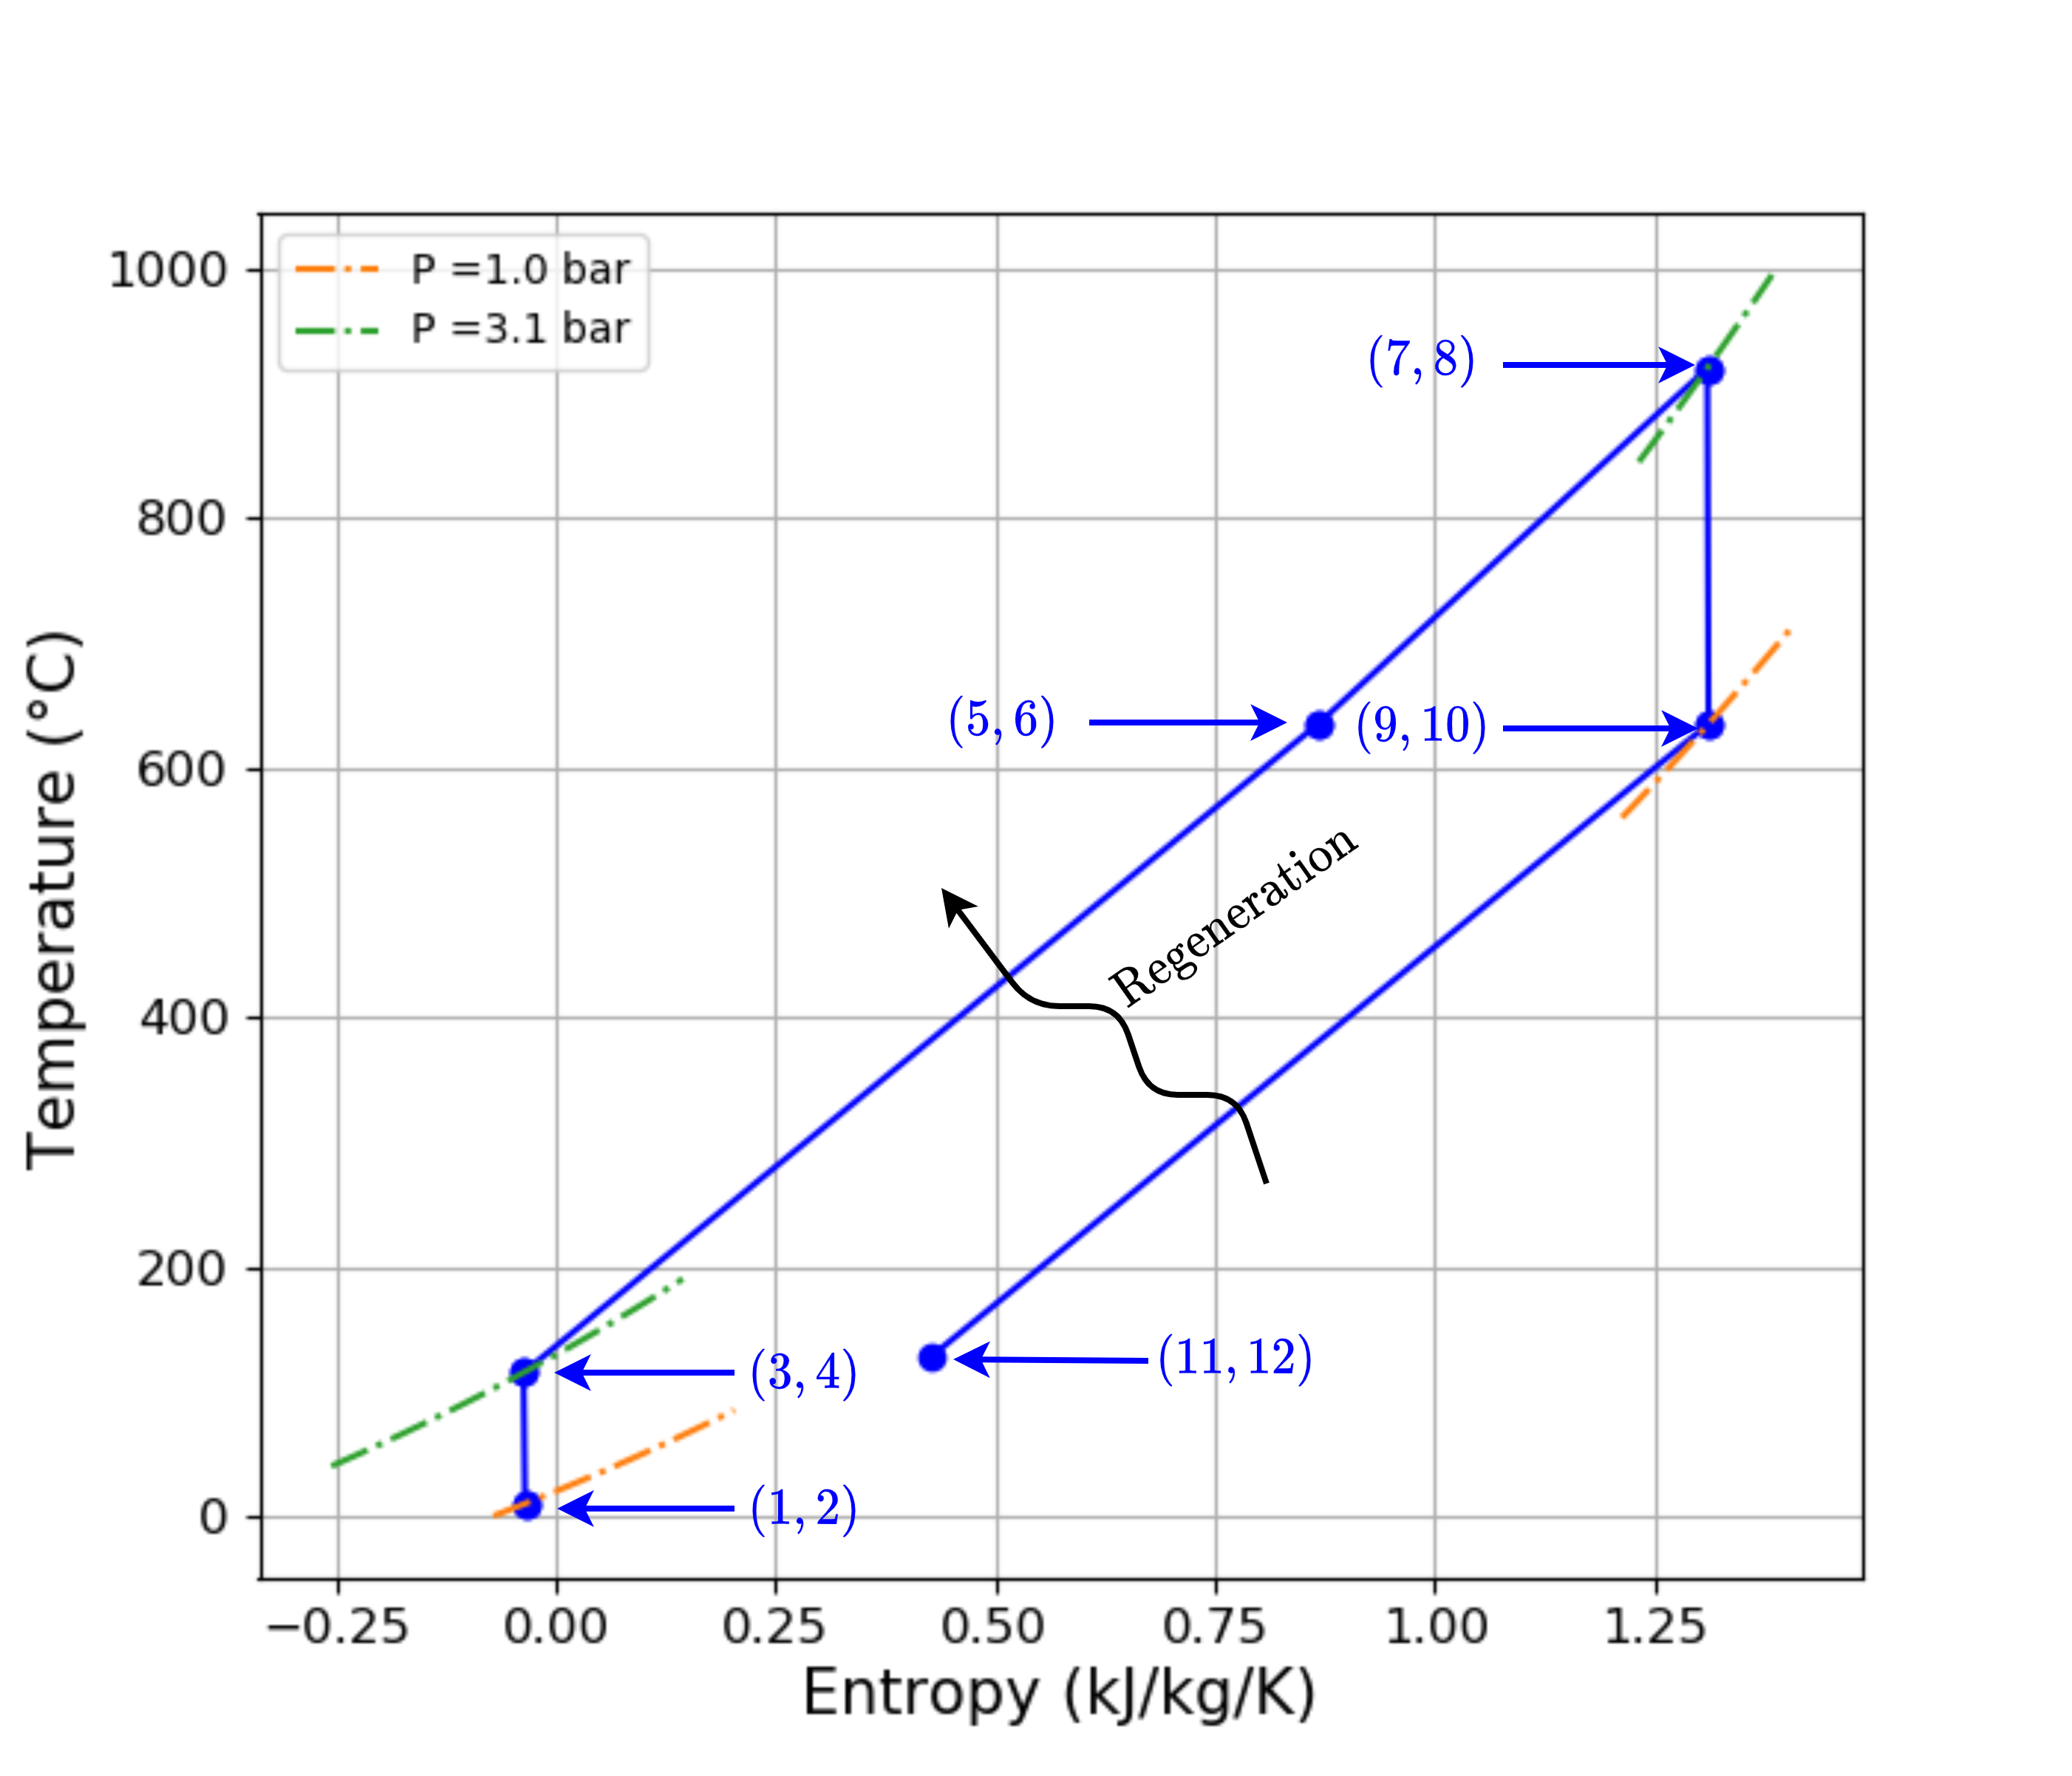
\includegraphics[width=\textwidth]{Ts_RGT}
         \caption{T-s diagram}
         \label{fig:C5_Ts_RGT}
     \end{subfigure}
        \caption{Thermodynamic diagrams - Regenerative Gas Turbine}
        \label{fig:C5_thermo_diagram_RGT}
\end{figure}

As shown in the T-s diagram, there is as expected a heat transfer from the hot gas to the cold air. This heat transfer allows using the available energy from the hot gas to heat-up the air from the compressor. Thanks to this heat transfer, the combustion chamber only needs to raise the temperature of the air from 630\degree C to 920\degree C. 

The reduction of the difference of temperatures between the inlet and the outlet of the combustion chamber results in a significant reduction of the consumption of fuel. For the same mass flow rate of air, the excess of air increased from 2 to 7. Thus, the mass flow rate of fuel $\dot{m}_{fuel}$ injected is decreased compared to the cycle without a regenerator.  

Thanks to the regenerator, the thermal efficiency of the cycle is really improved. Indeed, from 24\% for the ideal GT cycle, the efficiency of the Regenerative Gas Turbine cycle is now 65\%. The net power output is here equal to 41.35 kW. 

It can be noticed that the net power produced by the RGT is slightly lower than for the Gas Turbine, while the work respectively absorbed and produced by the compressor and the turbine remains identical. The reason is that the gas mass flow rate in the turbine is smaller due to the reduction of the amount of fuel injected in the combustion chamber. Therefore, the power produced during the expansion is a little bit smaller than previously.

\begin{figure}[h]
    \centering
    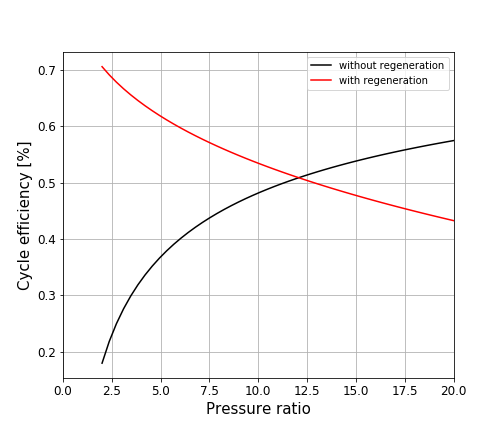
\includegraphics[width=0.5\textwidth]{Chapitre_5/Images/Efficiency_ideal_Brayton_regen.png}
    \caption{Thermal efficiency of GT vs. RGT}
    \label{fig:C5_eff_RGT-GT}
\end{figure}

The addition of the regenerator is only interesting when the pressure ratio involved is relatively small. Indeed, it can be demonstrated that the thermal efficiency of the RGT cycle varies as the inverse of the pressure ratio. On the other hand, the efficiency of the Gas Turbine cycle without regenerator increases with the pressure ratio. 

The Figure \ref{fig:C5_eff_RGT-GT} shows that, for a pressure ratio beyond 12.5, the cycle with regenerator has a thermal efficiency lower than the cycle without regenerator. 

\section{Intercooler-Regenerative-Reheat GT}
\quad\ The two cycles described previously are characterized by the usage of one compressor and one turbine. However, it happens that for some applications, the pressure ratio between the high and the ambient pressures is too large to be handled by one stage of turbomachines.

A type of Gas Turbine that is often considered to response to this problem is the Intercooler-Regenerative-Reheat Gas Turbine (IRHGT). For the IRHGT, the compression and the expansion are split between a low pressure (LP) and high pressure (HP) compressor and turbine (respectively). The low-pressure and high-pressure compressors and turbines are usually on the two different shafts due to the difference of rotational speed. The IRHGT cycle is depicted in the Figure \ref{fig:C5_IRHGT}.


\begin{figure}[h]
\centering
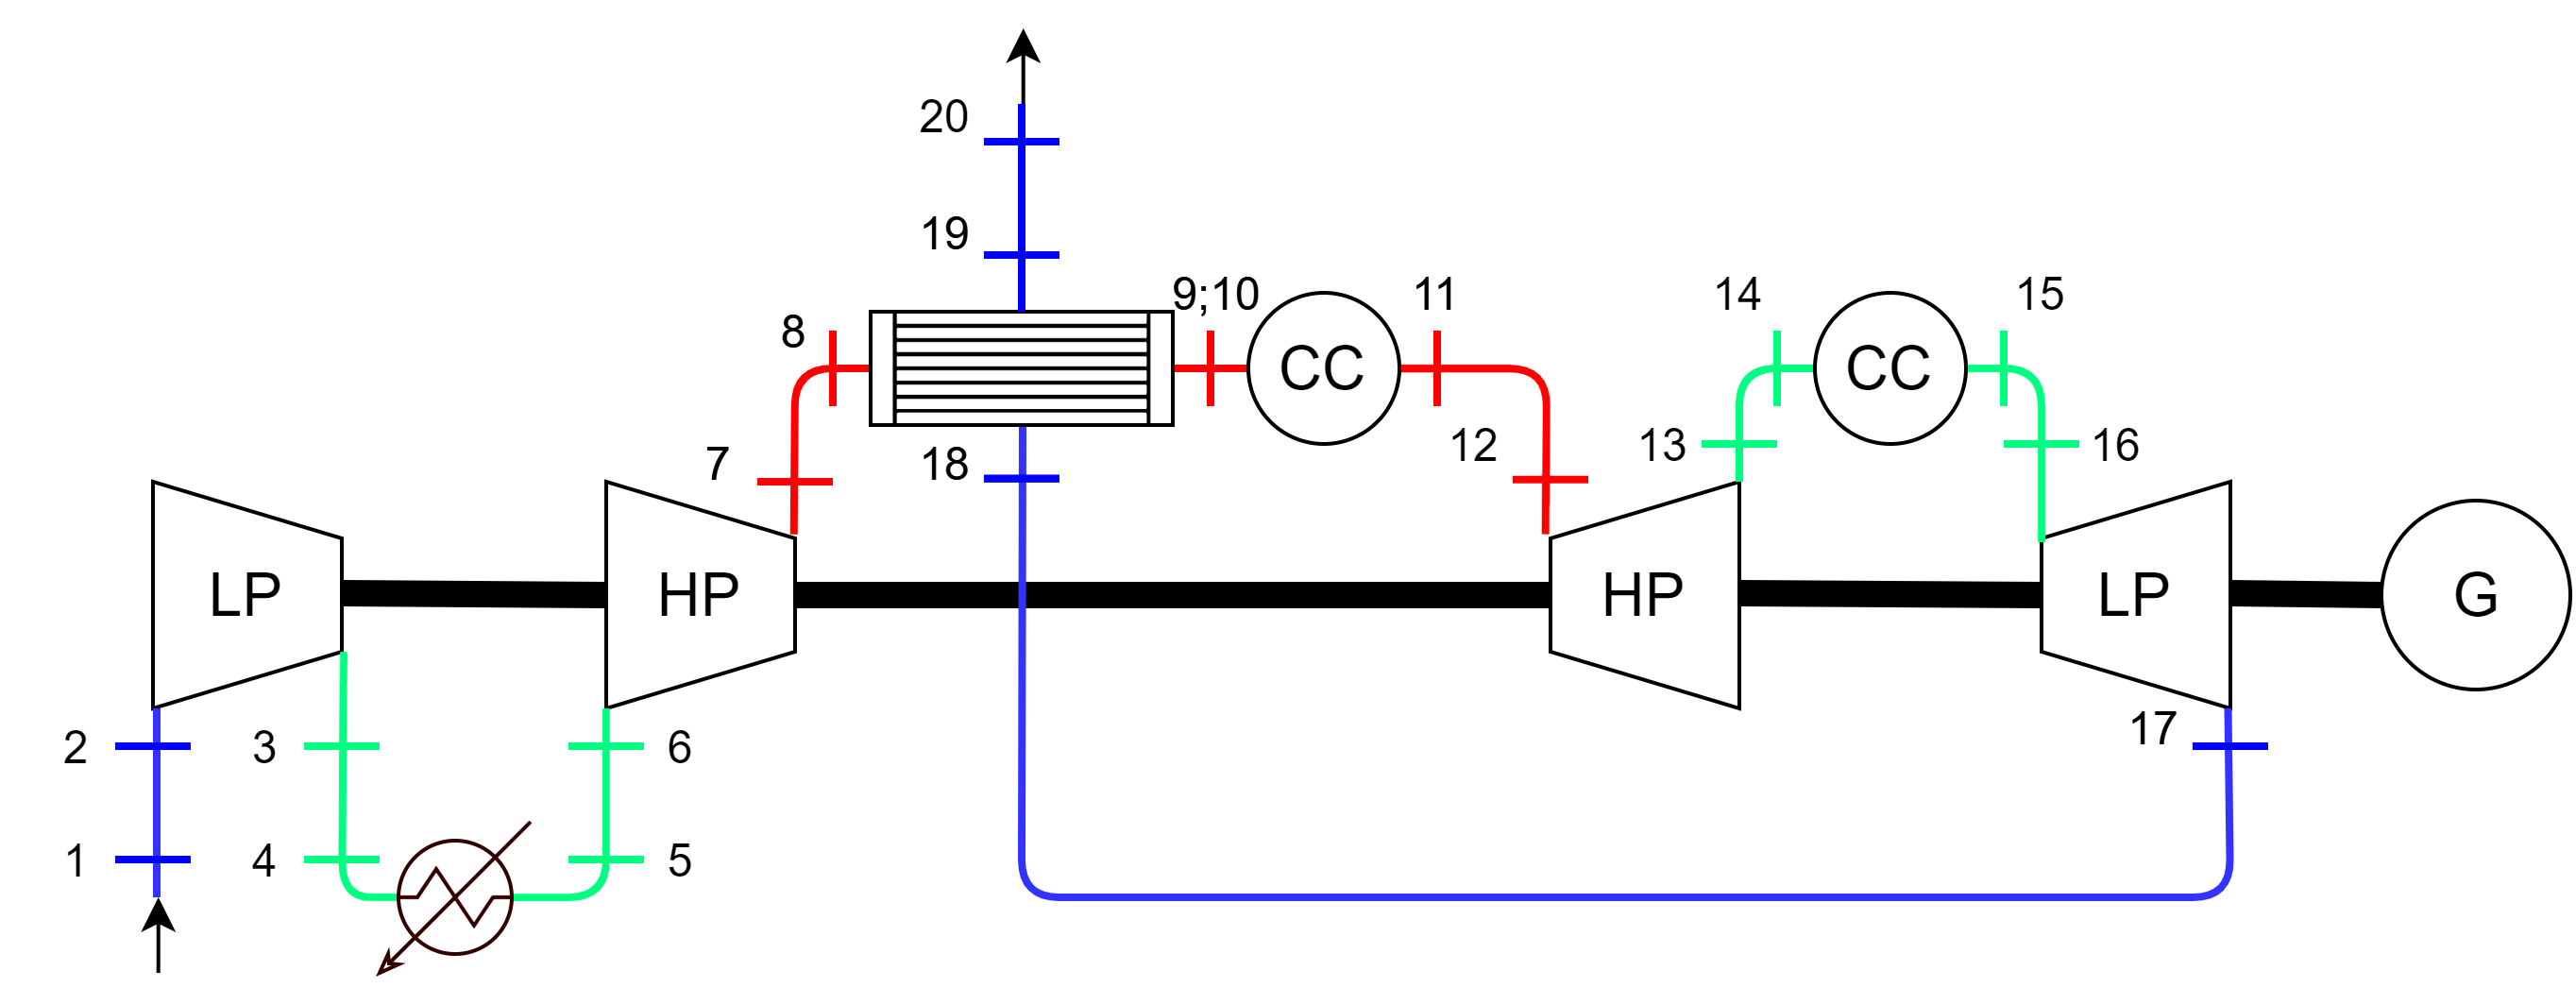
\includegraphics[scale=0.15]{IRHGT}
\caption{Intercooler-Regenerative-Reheat GT (IRHGT)}
\label{fig:C5_IRHGT}
\end{figure}

Between the two compression stages, a water heat exchanger called intercooler is installed to cool down the compressed air from the LP compressor before going into the HP compressor. The addition of an intercooler will allow to increase the \textbf{density} of the compressed thanks to the cooling. Indeed, when the air is compressed, its temperature is increased. However, at the same pressure, a hot gas will have a smaller density than cold gas. 

The opposite reasoning stands for the two stages of expansion. After the first stage, the expanded gas enters a second combustion chamber to be reheated. The reheat is performed to increase the \textbf{specific volume} of the gas before entering the low-pressure turbine. 


The p-v and T-s diagrams have been drawn for the case of an ideal IRHGT cycle. The two diagrams are in the Figures \ref{fig:C5_pv_IRHGT} and \ref{fig:C5_Ts_IRHGT}.

\begin{figure}[h]
     \centering
     \begin{subfigure}[b]{0.4\textwidth}
         \centering
         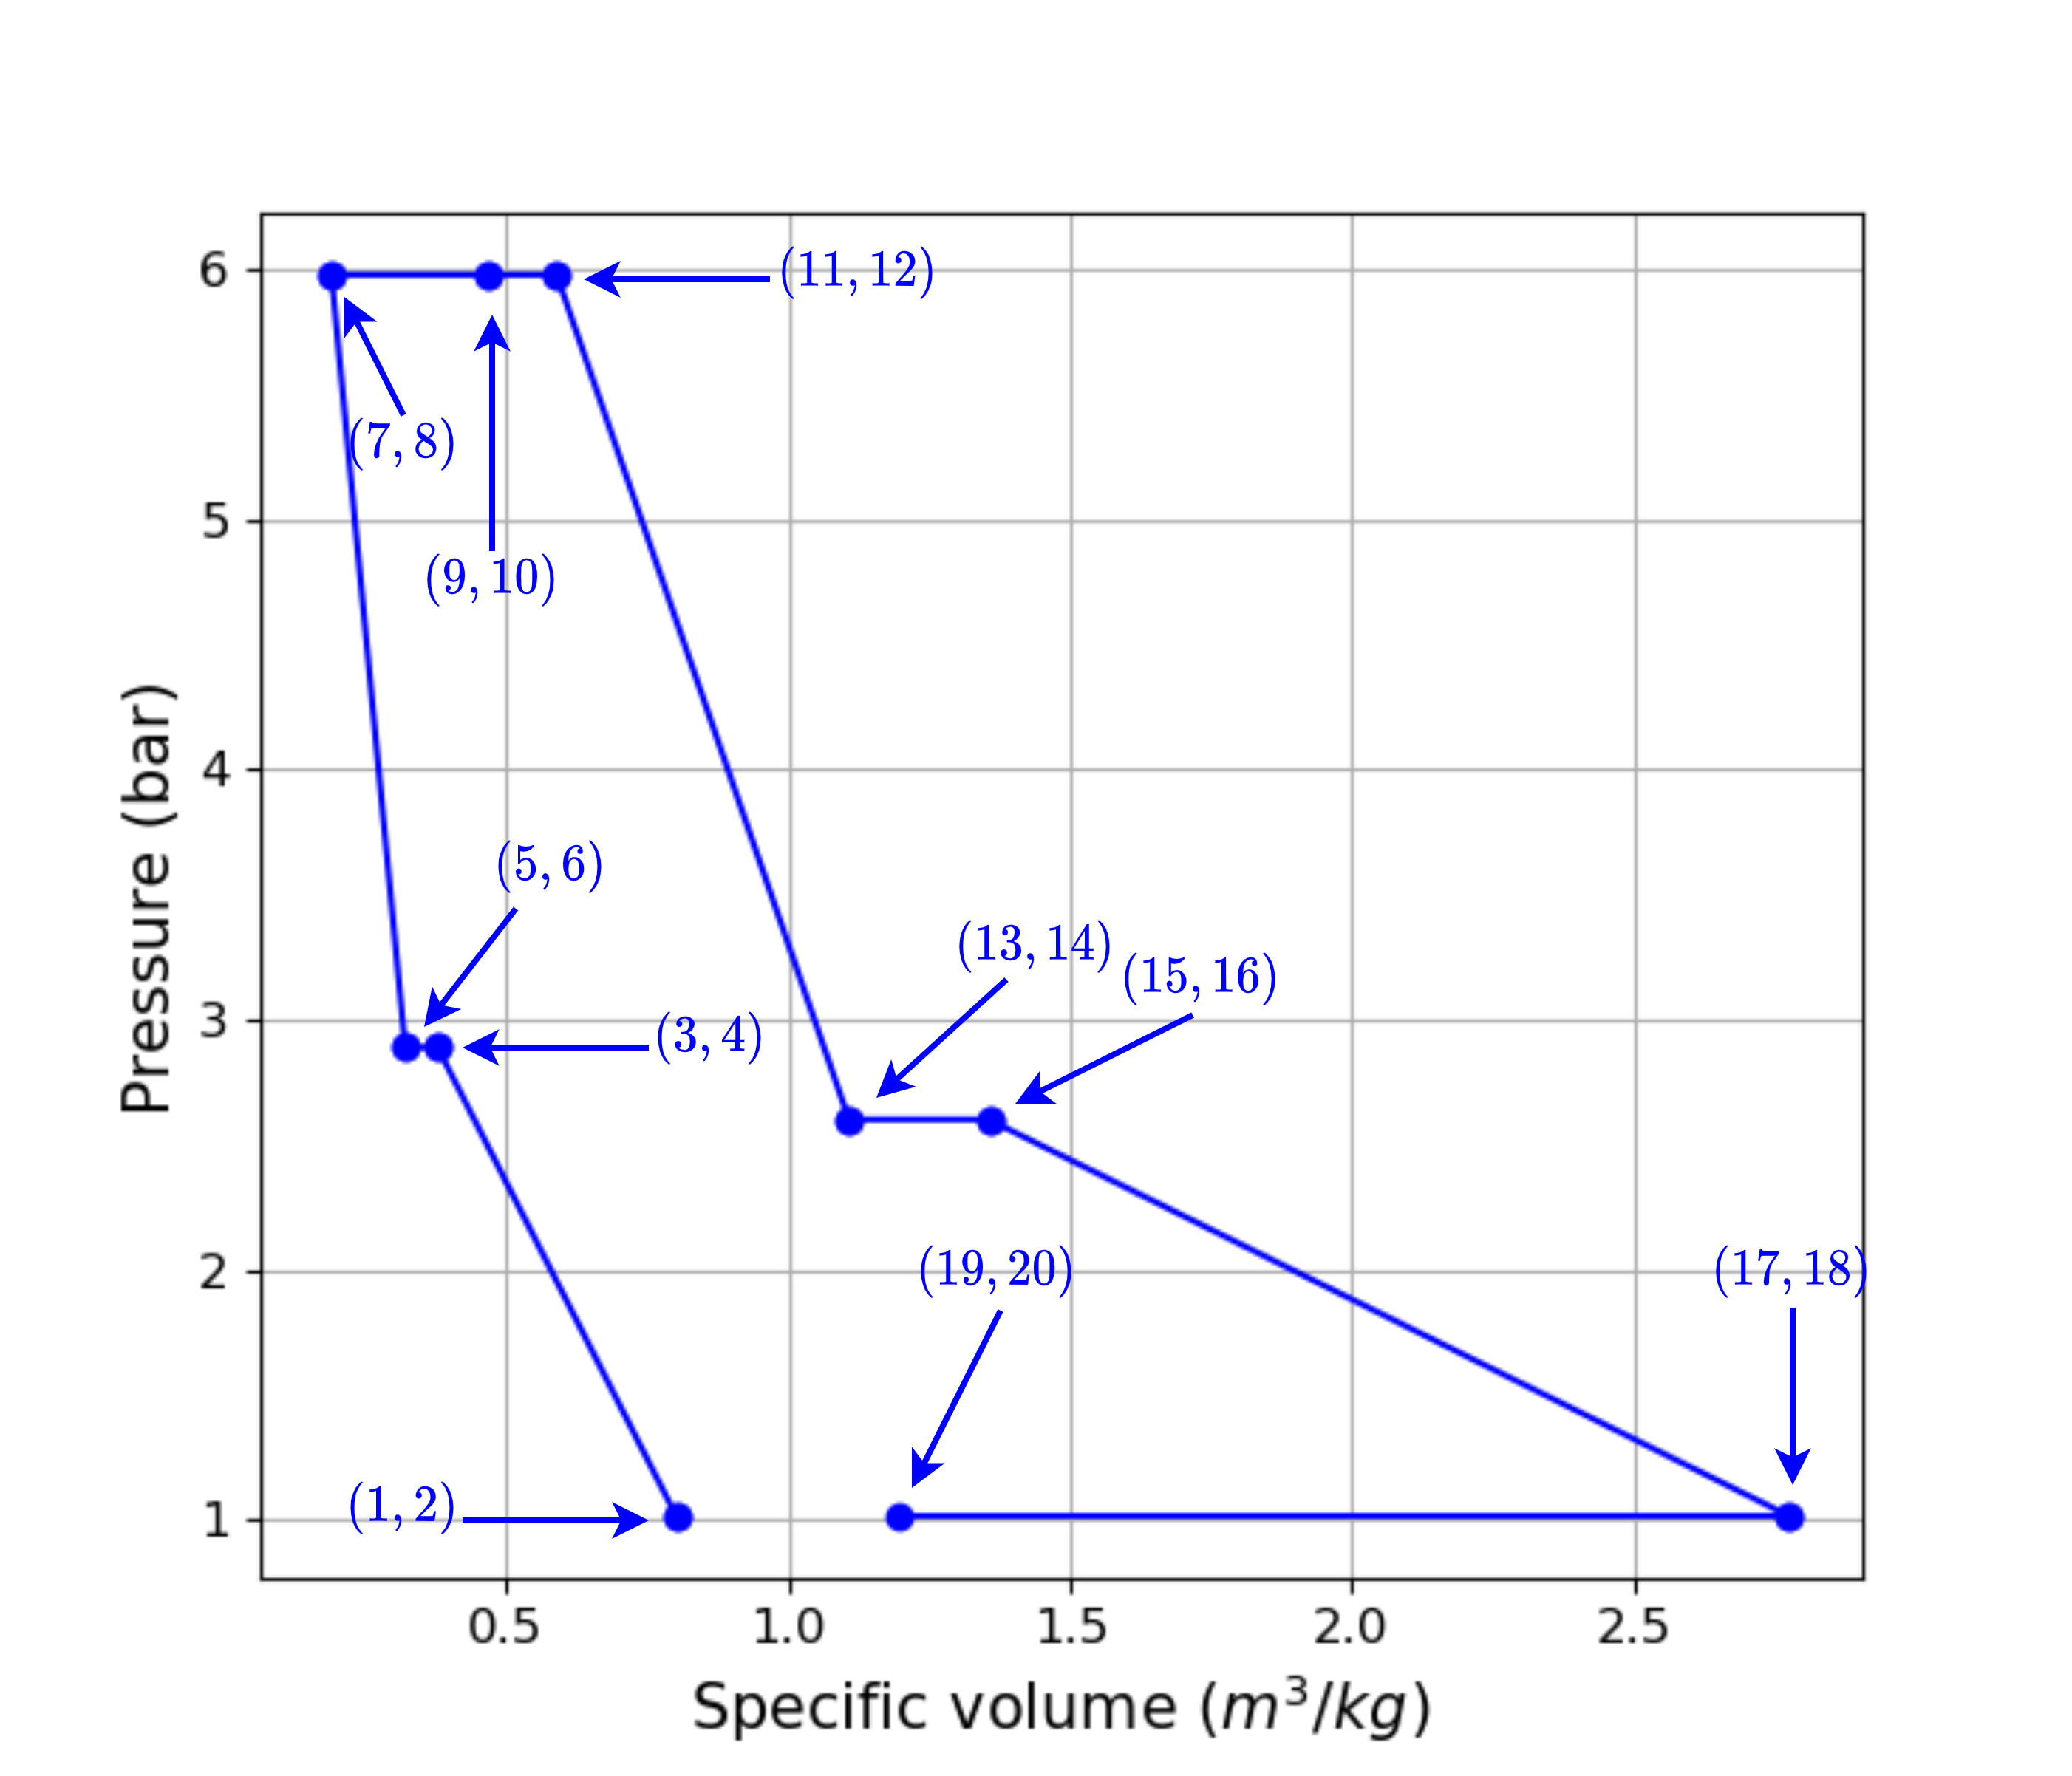
\includegraphics[width=\textwidth]{pv_IRHGT}
         \caption{p-v diagram}
         \label{fig:C5_pv_IRHGT}
     \end{subfigure}
     \begin{subfigure}[b]{0.4\textwidth}
         \centering
         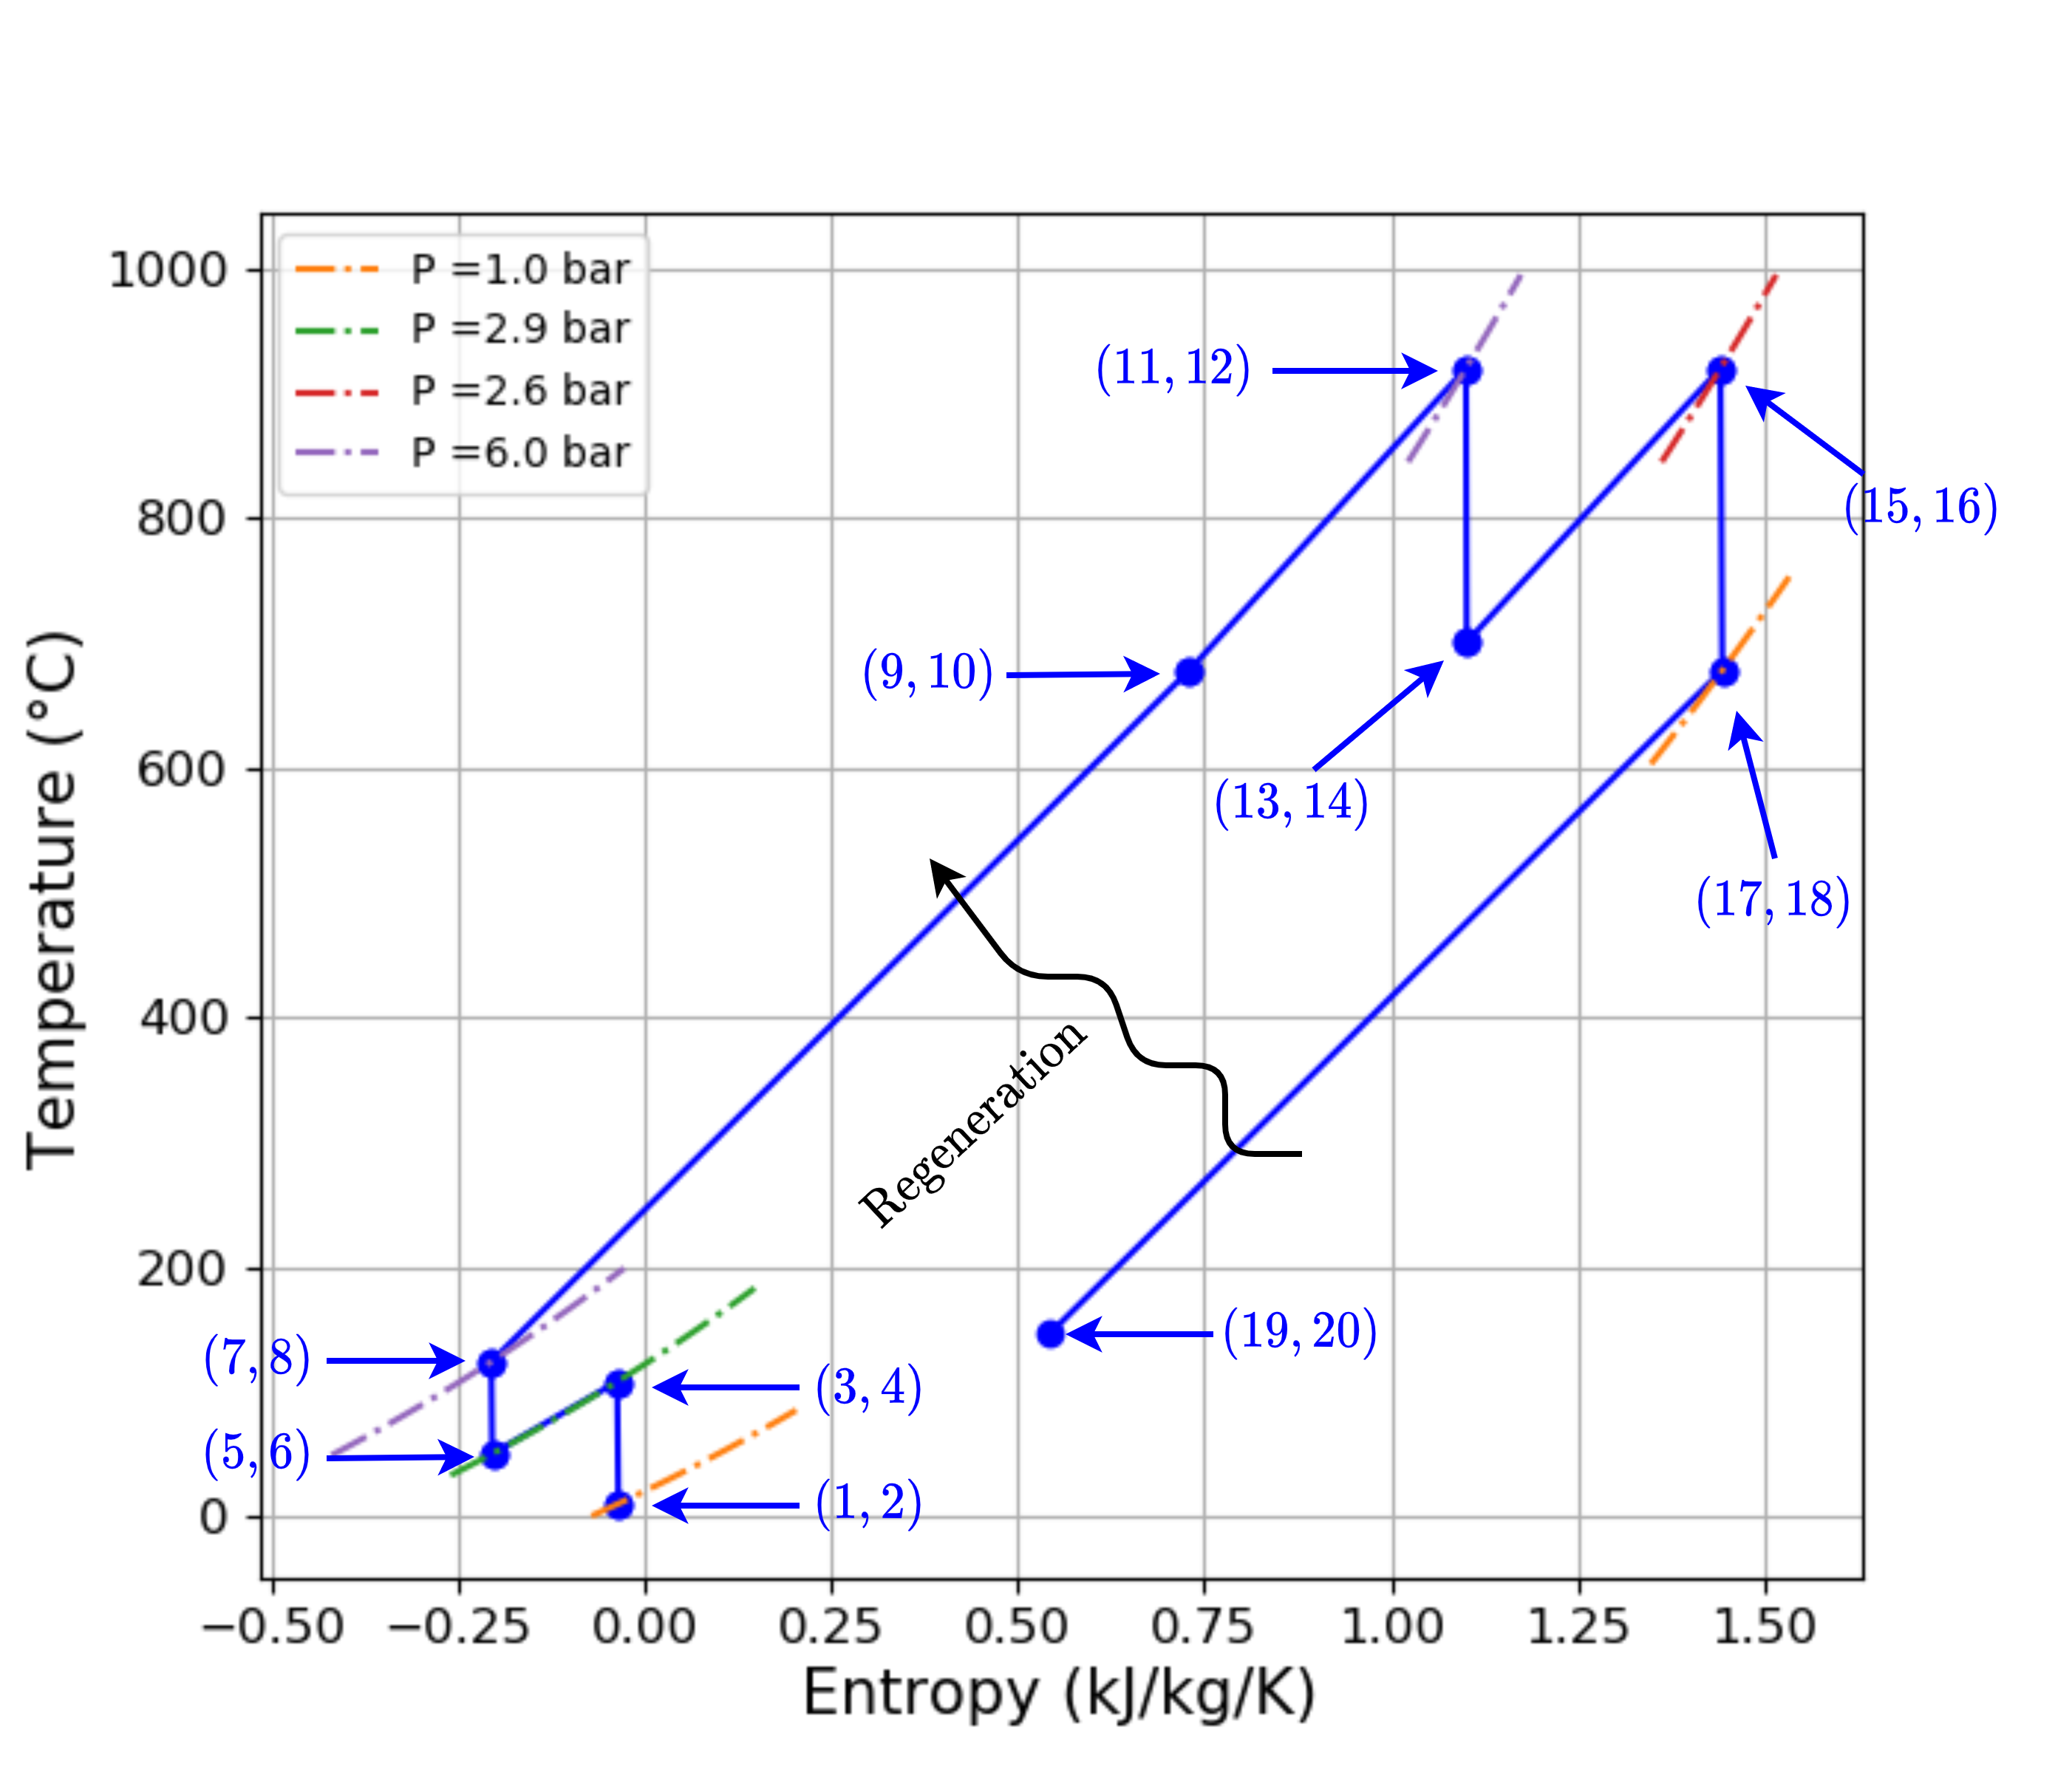
\includegraphics[width=\textwidth]{Ts_IRHGT}
         \caption{T-s diagram}
         \label{fig:C5_Ts_IRHGT}
     \end{subfigure}
        \caption{Thermodynamic diagrams - Intercooler-Regenerative-Reheat Gas Turbine}
        \label{fig:C5_thermo_diagram_IRHGT}
\end{figure}

As depicted in the diagram T-s, four levels of pressure are involved. First, there is the low-pressure (LP) corresponding to the pressure of the environment. From the state \textbf{2} to the state \textbf{3}, the LP compressor will raise the pressure of the air to a medium pressure (MP) level. 

At the end of this first stage of compression, the air that has been heated due to the compression is cooled down to 50\degree C using an intercooler. It results from the cooling a reduction of the entropy of the air. Then, the cooled air is compressed again by a high pressure (HP) compressor to reach the target pressure of 6 bars.

After the two stages of compression, the air is first heat-up in the regenerator by the hot gas from the LP turbine, then by the high-pressure combustion chamber to reach to desired Turbine Inlet Temperature (or TIT) of 920\degree C. 

The expansion from 6 bar to 1 bar is split into two stages. Here, there is a degree of free regarding the choice of the expansion ratio of the HP and LP turbines. One of the can be fixed in order to maximized the efficiency or the power output of the system. 

After the expansion from the high pressure to a medium pressure is done, the expanded gas is reheated to the TIT of 920\degree C using a second combustion chamber. Then, the exhaust gas goes through the low-pressure turbine to decrease its pressure to 1 bar. Finally, the remaining high quality heat in the gas is used to heat-up the air from the high-pressure compressor.

For this particular IRHGT cycle, the thermal efficiency of the ideal IRHGT is equal 65\% and the associated net power output of 68 kW. It can be noticed that the efficiency of the cycle is identical to the one of the RGT cycle. However, the net power produced by this enhanced cycle is 26 kW higher. 

\section{Brayton cycle - variants}
%%%%%%%%%%%%%%%%%%%%%%%%%%%%%%%%%%%
%%%%%                         %%%%%
%%%%%      <<Variants>>       %%%%%
%%%%%                         %%%%%
%%%%%%%%%%%%%%%%%%%%%%%%%%%%%%%%%%%
\quad\ Aside the Gas Turbine, two variants have been described in the previous section. However, there exists many other configurations that can be studied. There exists Brayton gas cycle where only the compression is staged, or cycle where the expansion is performed before the combustion. This variant is called Externally-Fired Gas Turbine (EFGT) and reduces the stress on the turbine induced by the fumes.

Also, once the fumes are at the exit of the cycle, it remains low quality heat (below 200\degree C except for the GT cycle) that can be used to heat-up water for sanitary usage.

The Table \ref{tab:C5_inputconfig} gives a non-exhaustive list of existing variant of the gas cycles. A diagram for each cycle can be found in the appendix\ref{annex:Brayton_variant}.
\begin{longtable}[c]{ll}
\caption{Variant of the Gas Turbine cycle}
\label{tab:C5_inputconfig}\\
\toprule
\textbf{Acronym} & \textbf{Type - Name}                   \\* \midrule
\endfirsthead
%
\endhead
%
\bottomrule
\endfoot
%
\endlastfoot
%
GT                           & Gas Turbine                                 \\
RGT                          & Regenerative Gas Turbine                    \\
IGT                          & Intercooler Gas Turbine                     \\
IHGT                         & Intercooler-Reheat Gas Turbine              \\
IRGT                         & Intercooler-Regenerative Gas Turbine        \\
IRHGT                        & Intercooler-Regenerative-Reheat Gas Turbine \\
EFGT                         & Externally-Fired Gas Turbine                \\* \bottomrule
\end{longtable}


\newpage
%%%%%%%%%%%%%%%%%%%%%%%%%%%%%%%%%
%% Chapitre 6:                 %%
%% Code structure   		   %%
%%%%%%%%%%%%%%%%%%%%%%%%%%%%%%%%%
\graphicspath{{Chapitre_6/Images/}}
\chapter{Model overview}\label{C6}
%%%%%%%%%%%%%%%%%%%%%%%%%%%%%%%%%%%
%%%%%                         %%%%%
%%%%% Introduction chapitre 5 %%%%%
%%%%%                         %%%%%
%%%%%%%%%%%%%%%%%%%%%%%%%%%%%%%%%%%
\quad\, In the chapter \ref{C5}, the Brayton cycle has been introduced by presenting two configurations. Also, it has been mentioned that many other configurations (illustrated in the annex \ref{annex:Brayton_variant}) exists to cover a large panel of applications. 

This chapter will be devoted to the description of the  Brayton cycle model. This model will only consider steady state operations. Thus, transient effects like the acceleration of the turbomachines or the heating up of the heat-exchangers will not be taken into consideration.
 

\section{Python language}
%%%%%%%%%%%%%%%%%%%%%%%%%%%%%%%%%%%
%%%%%                         %%%%%
%%%%%  <<Python language>>    %%%%%
%%%%%                         %%%%%
%%%%%%%%%%%%%%%%%%%%%%%%%%%%%%%%%%%
\quad\, Python is a computing language that was created by Guido van Rossum at the Centrum Wiskunde \& Informatica (CWI - \url{https://www.cwi.nl}) in the early 1990s. Starting 1995, G. van Rossum continued to work on Python at the Corporation for National Research Initiatives (CNRI - \url{https://www.cnri.reston.va.us/}). Since the very first release, the language was open source. This means that the source code was accessible to anyone. 

From this time, Python progressively gained in popularity, and the community participating in the development of the software didn't stop growing. Today, this language is used by many companies and for many types of applications. Indeed, this programming language is used for website creation, machine learning, automation, etc. 

Since Python is an open source language, it lives thanks to its community which creates and shares libraries. Indeed, what has already been implemented in the past can be freely used by the other users. Moreover, new users can easily start developing under Python thanks to huge amount of guide and documentation to starting learning about the Python language.

Also, Python is a programming language that allows the object-oriented programming. This paradigm consists in the definition of blocks of code (called objects) which are able to interact through relations, defined in order to solve a given problem. This allows creating computer code that can evolve through the times. 

\section{Model structure}
%%%%%%%%%%%%%%%%%%%%%%%%%%%%%%%%%%%
%%%%%                         %%%%%
%%%%% <<Structure of the>>    %%%%%
%%%%%      <<model>>          %%%%%
%%%%%                         %%%%%
%%%%%%%%%%%%%%%%%%%%%%%%%%%%%%%%%%%
\quad\, The focus of this section is the description of the structure of the computer code itself. The program is separated into multiple blocks which can interact between each other. Before explaining the role of each of these blocks, the global structure of the program will be given.

\subsection{Input file}
\quad\, To start the program, the user has to provide an input file that will contain all the required information to execute the program. The structure of the inputs follows the YAML scheme which is a language that allows storing data in a structure and readable ways for the human\footnote{YAML stands for \textbf{Y}AML \textbf{A}in't \textbf{M}arkup \textbf{L}anguage.} . The strength of such language is that any data can be expressed under an arbitrary name. 

When the python code read the file, the file will be interpreted as a nested dictionary. A dictionary in Python can be considered as a table that can contain elements of different types. In a nested dictionary, some of these elements are also dictionary.

Here the YAML file that is given to the program is composed of four dictionaries respectively identified by the names "Type", "Selection", "Input" and "Extra". An example of an input files is given in the appendix \ref{annex:yaml}. 

\subsubsection{Type}
\quad\ The dictionary "Type" is composed of only one field that specified which variant of the Brayton cycle is going to be studying. By specifying one of the names listed in the Table \ref{tab:C5_inputconfig}, the program will now the variant to load in the memory.

\subsubsection{Selection}
\quad\ Then, the second dictionary "Selection" is used to specialize the variant and is composed of boolean elements. The reading of this dictionary will say to the program what extra data are expected to be found in the dictionary ''Extra''.
\newpage
The first element "WHX" of this dictionary is about the choice to add a water heat exchanger to recover part of the temperature in the fumes. If the field is set to \textit{true}, the following inputs will be required:
\begin{itemize}
    \setstretch{1}
    \item $\varepsilon_{whx}$: Efficiency of the water heat exchanger (\%)
    \item $T_{whx,water,in}$, $T_{whx,water,out}$: Inlet and outlet temperature of the water (\degree C)
    \item $P_{whx,water, in}$: Inlet pressure of the water (\degree C)
    \item $Dp_{whx,water}$, $Dp_{whx,gas}$: Water and gas nominal pressure drops (\%)
\end{itemize}

Then, the field "MAP" gives the choice to use performance maps (provided by the user) for the compressor and the turbine. If set to \textit{true}, the absolute path to the performance maps and the rotational speed of the turbomachines have to be specified. The performance maps are given as Excel sheets where each row corresponds to an operating point characterized by \(\dot{m}_{corr}\), \(\Pi_{tt}\), \(N_{corr}\) and \(\eta_{is}\).

By default, the maps are not used. Instead, the following inputs are asked to be able to characterize the compressor and the turbine:

\begin{itemize}
\setstretch{1}
    \item $\eta_{is,c}$ and $\eta_{is,t}$: Isentropic efficiency of the compressor and the turbine (\%)
    \item $\Pi_{tt,c}$: Total to total compression ratio (-)
    \item $TIT$: Turbine Inlet Temperature (\degree C)
\end{itemize}

The parameter "VAR\_DP" included in the dictionary "Selection" is used to take into account the variation of the pressure drops with the mass flow rate. If this feature is desired, the nominal mass flow rate associated to the nominal pressure drop has to be specified.  

Similarly, the last parameter "Var\_EFF" in the dictionary allows taking into account the heat exchanger efficiency dependency to the temperature and mass flow rate of both flows. If this option is chosen, the nominal mass flow rate and the nominal inlet/outlet temperatures for which the heat exchanger has the specified efficiency are required.

\subsubsection{Input}
\quad\ This third dictionary contains all the default parameters that are required to assess the performance of the selected variant of the Brayton gas cycle. As an example, the Table \ref{tab:C6_inputRGT} includes the inputs that has to be specified.

\begin{longtable}[c]{@{}llc@{}}

\caption{Input - Regenerative Gas Turbine (RGT)}
\label{tab:C6_inputRGT}\\
\toprule
\textbf{Input}                        & \textbf{Abbreviation} & \textbf{Unit} \\* \midrule
\endfirsthead
%
\endhead
%
\bottomrule
\endfoot
%
\endlastfoot
%
Reference temperature                 & $T_{ref}$                                 & \degree C     \\
Reference pressure                    & $P_{ref}$                                 & Pa            \\
Ambient temperature                & $T_{amb}$                                 & \degree C     \\
Ambient pressure                      & $P_{amb}$                                 & Pa            \\
Fuel temperature                      & $T_{fuel}$                                & \degree C     \\
Mass flow rate of air                 & $\dot{m}_{air}$                           & kg/s          \\
Air factor                            & $\lambda$                                 & -             \\
\rowcolor[HTML]{FFFFC7} 
Compression ratio                     & $\Pi_{tt,c}$                              & -             \\
\rowcolor[HTML]{FFFFC7} 
Turbine Inlet Temperature             & $TIT$                                     & \degree C     \\
\rowcolor[HTML]{FFFFC7} 
Compressor isentropic efficiency      & $\eta_{is,c}$                             & \%            \\
\rowcolor[HTML]{FFFFC7} 
Turbine isentropic efficiency         & $\eta_{is,t}$                             & \%            \\
Combustion efficiency                 & $\eta_{cc}$                               & \%            \\
Shaft mechanical efficiency           & $\eta_{shaft}$                            & \%            \\
Generator efficiency                  & $\eta_{gen}$                              & \%            \\
Regenerator efficiency                & $\varepsilon_{re}$                        & \%            \\
Combustion chamber pressure drop      & $Dp_{cc}$                                 & \%            \\
Regenerator pressure drop (hot side)  & $Dp_{re,H}$                               & \%            \\
Regenerator pressure drop (cold side) & $Dp_{re,C}$                               & \%            \\
Duct pressure drop                    & $Dp_{duct}$                               & \%            \\
Chimney pressure losses               & $\Delta p_{chimney}$                      & Pa            \\
Fuel composition                      & $Fuel_{comp}$                             & -             \\
Air composition                       & $Air_{comp}$                              & -             \\* \bottomrule
\end{longtable}

The inputs emphasized in yellow in the Table \ref{tab:C6_inputRGT} are ones that are not used if the map of the compressor and the turbine are used. The air factor $\lambda$ is used to initiate the iterative search of the mass flow rate of fuel in the program. Any value greater than one is acceptable. Further explanations are given in the following section.


\subsubsection{Extra}
\quad\ The last part of the YAML file is dedicated to the extra inputs that have to be provided based on the choices made in the "Selection" part. 

\subsection{Flow chart of the model}
\quad\,  The previous section detailed the structure of the input file to be provided at the start of the program.  
\begin{figure}[h]
\centering
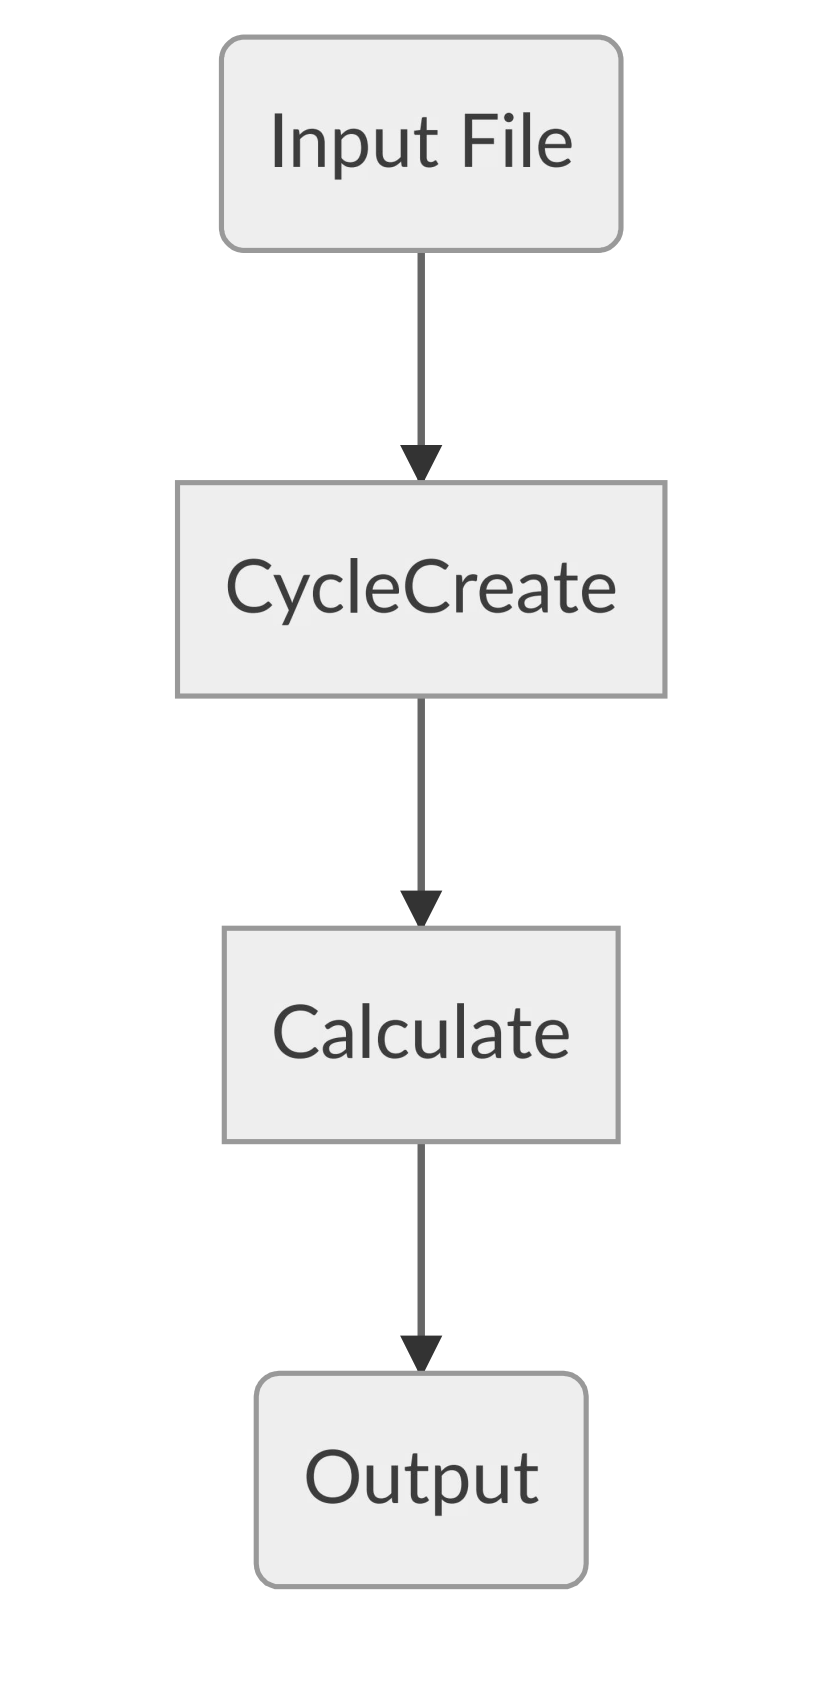
\includegraphics[width=0.2\textwidth]{Chapitre_6/Images/GeneralFlowChart.png}
\caption{General flow chart of the program}
\label{fig:C6_flowchart}
\end{figure}

Once provided, the program will first read the "Type" field to select the desired configuration. This is done by the function \textit{CycleCreate} that will create the model associated to the configuration selected. This function, for which the scheme is given in the Figure \ref{fig:C6_cyclecreate}, first parses the inputs file to extract the four dictionaries "Type", "Selection", "Input" and "Extra". 

\begin{figure}[h]
    \centering
    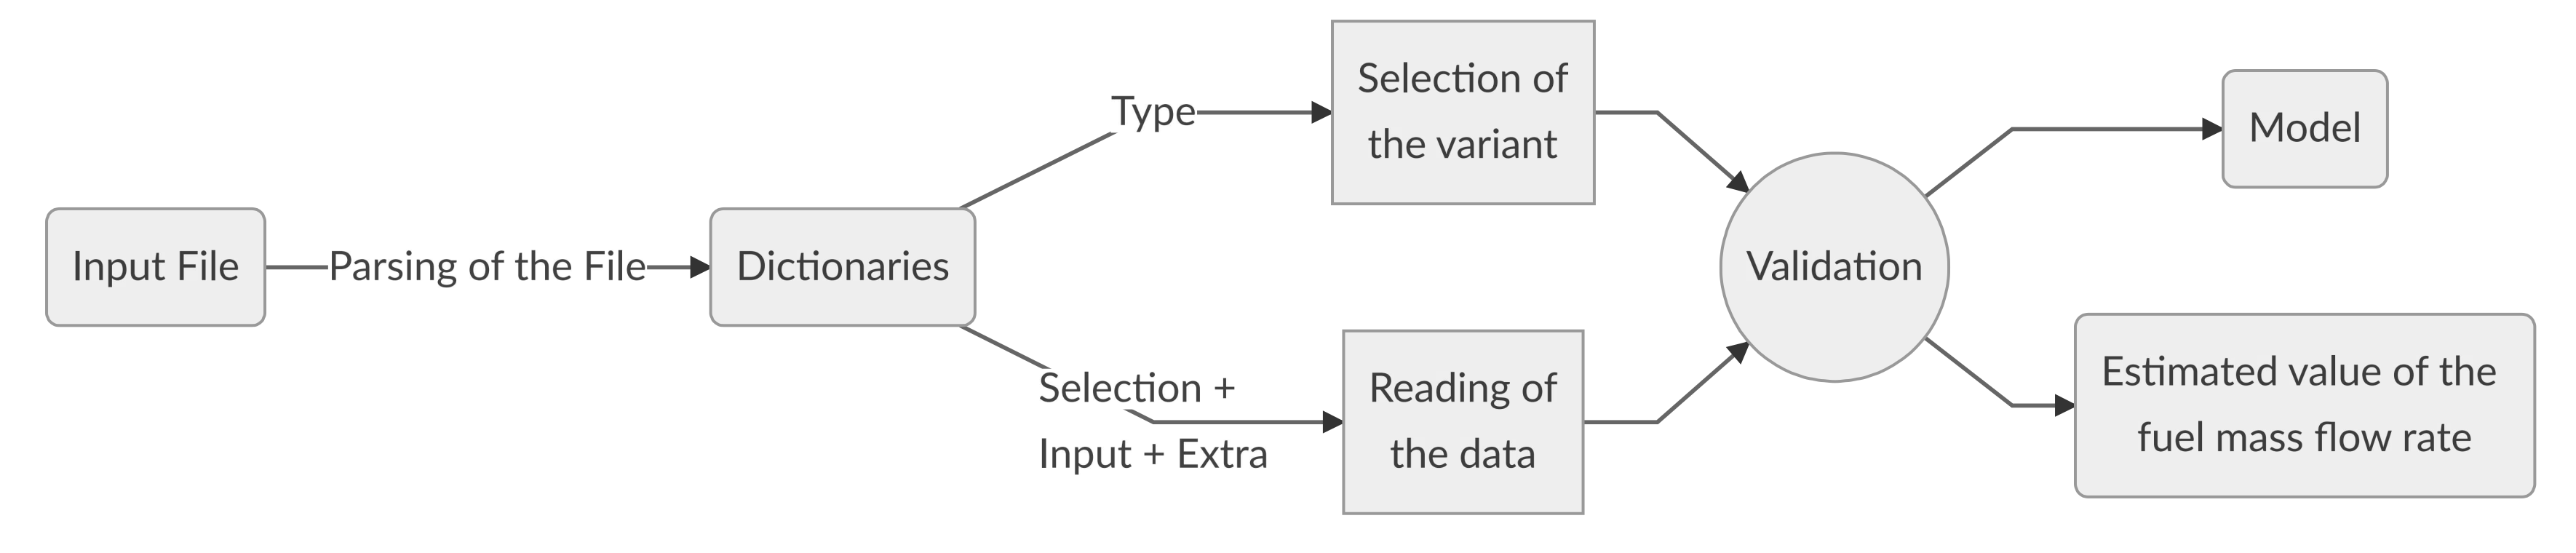
\includegraphics[width=0.9\textwidth]{Chapitre_6/Images/CycleCreate.png}
    \caption{Scheme of the function \textit{CycleCreate}}
    \label{fig:C6_cyclecreate}
\end{figure}
Then, all the data are read and stored. Based on the choice made in the "Selection" section, the function will search information in the dictionary named "Extra". 
Finally, the function validates the inputs read to ensure that the program will run without leading to an error induced by missing or wrong data. After this step of verification, the model for the selected configuration is created.

Once the model created, it is provided to the \textit{Calculate} function. The scheme of this function is provided in the Figure \ref{fig:C6_calculate}.

\begin{figure}[h]
    \centering
    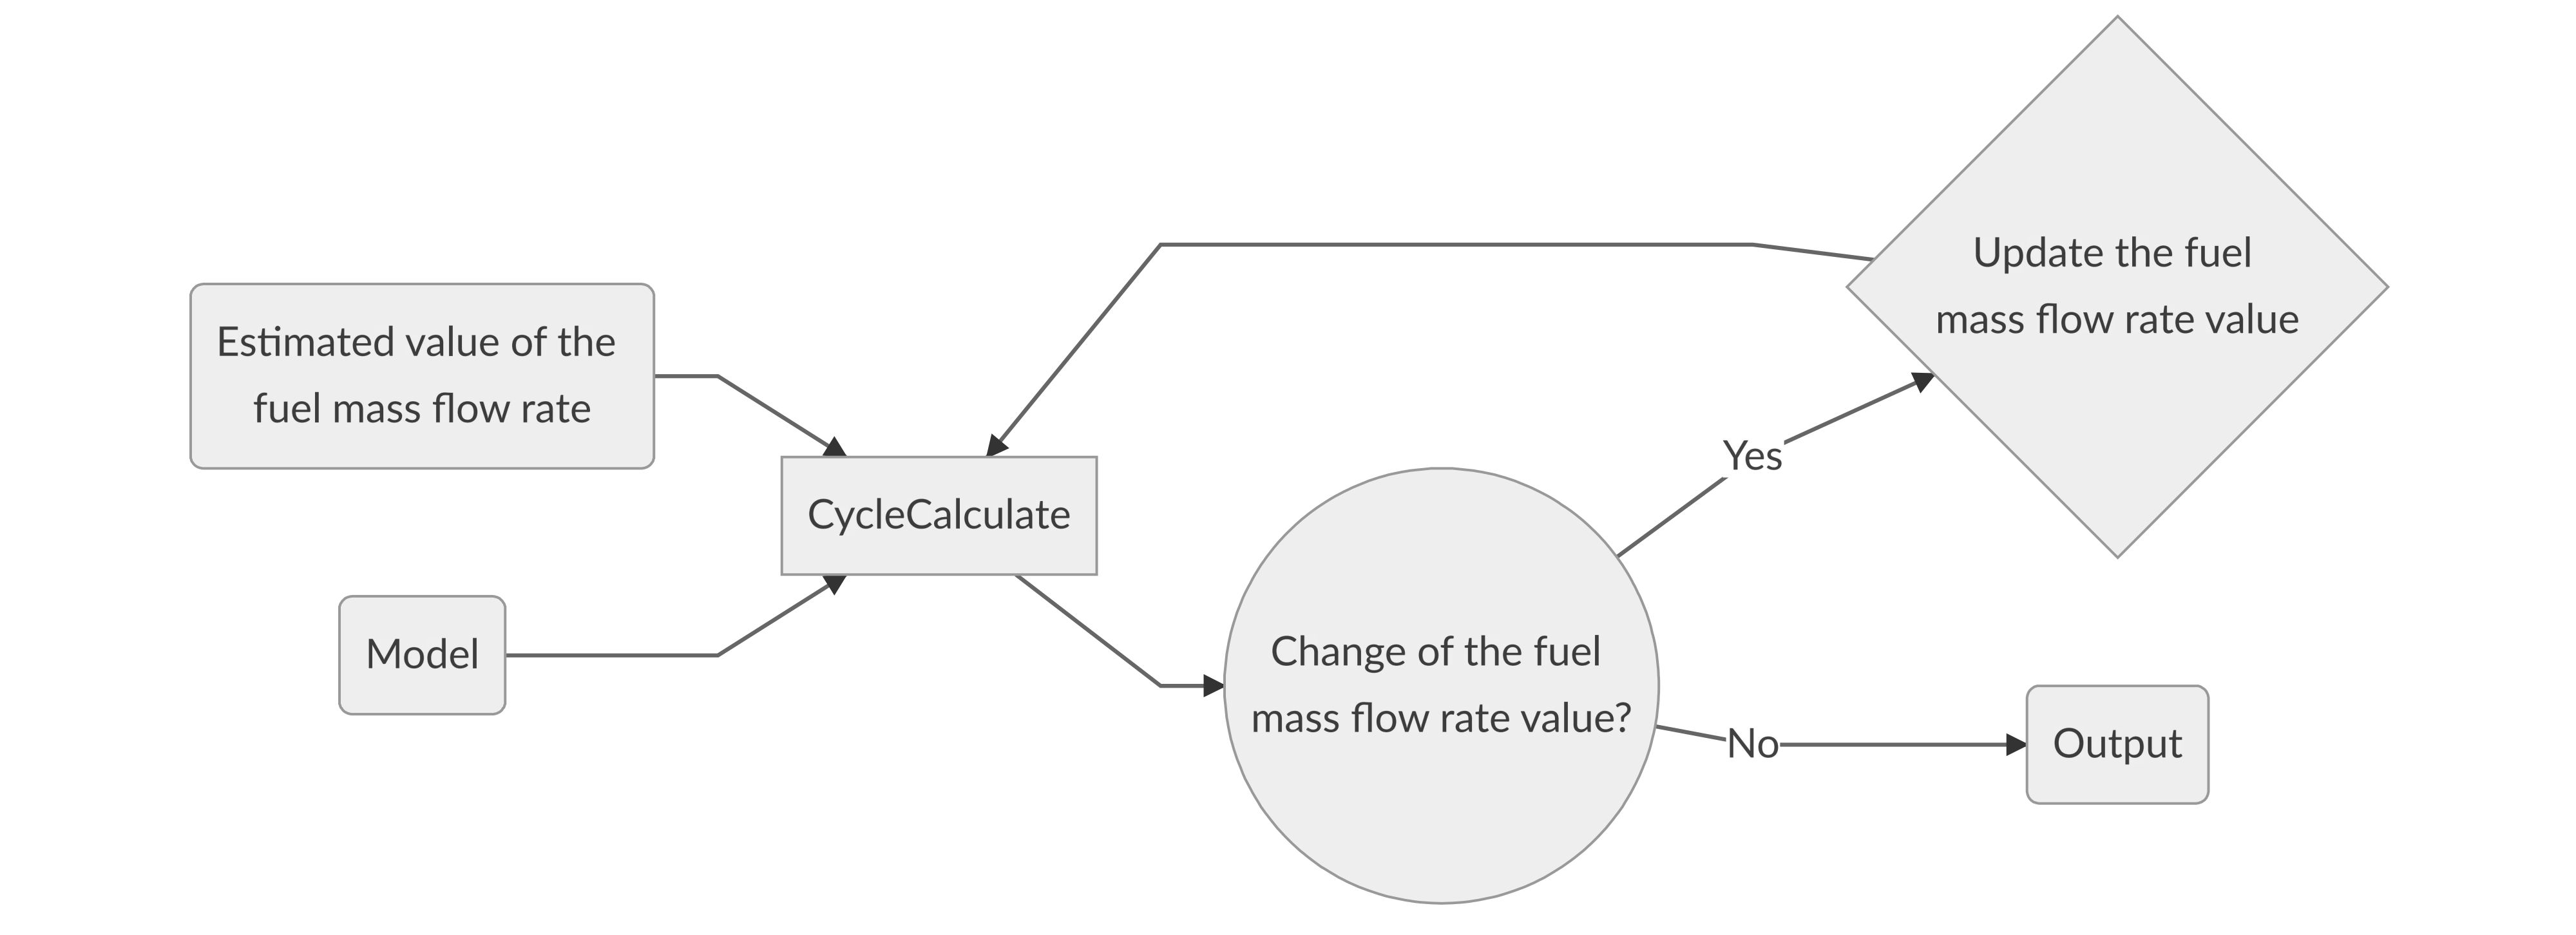
\includegraphics[width=0.9\textwidth]{Chapitre_6/Images/Calculate.png}
    \caption{Scheme of the function \textit{Calculate}}
    \label{fig:C6_calculate}
\end{figure}

Here, an initial guess for the mass flow rate of fuel injected into the combustion chamber is required. This guess value is obtained using the mass flow rate of air and the air factor $\lambda$. 

Then, the function \textit{CycleCalculate} is called. The structure of this function varies from one configuration to the other. Nevertheless, \textit{CycleCalculate} is a function that follows the path taken by the actual flow in the cycle. This function is composed of blocks (or objects) representing the elements constituting the cycle. Based the variant chosen, the order of these blocks will be different.  

Once the Brayton cycle completed, the value of the mass flow rate of fuel has been updated. If its value is different from the initial guess, the latter is updated and the function \textit{CycleCalculate} is called again. If the two values are really closed from one to the other, the program exits the loop and provides some outputs.

The outputs of the program are:

\begin{itemize}
\setstretch{1}
    \item The temperature, pressure, enthalpy, entropy and density for the defined states.
    \item The mass flow rate of fuel and the air factor.
    \item The power produced or consumed by the different elements.
    \item The efficiency of the different elements.
    \item The efficiency of the cycle.
    \item The corrected and reduced quantities associated to the turbomachines.
\end{itemize}

The interest of these outputs is to be able to quantify the performance of the cycle and to adapt some of the input in order to reach the desired results. For instance, for a gas turbine the target value for air factor is often in the neighboring of 8-10. Also, the TIT is in practice limited by the material constituting the turbine blades. Indeed, a large temperature would destroy the turbine by reaching the melting temperature of the material.

Next chapter will present the implementation method of each element constituting the cycle. For each of those, the functions involved will be defined and explained. Also, some links with the theoretical notions seen in chapters \ref{C2}, \ref{C3} and \ref{C4} will be created.






 
\newpage
%%%%%%%%%%%%%%%%%%%%%%%%%%%%%%%%%
%% Chapitre 7:                 %%
%% Brayton cycle modeling      %%
%%%%%%%%%%%%%%%%%%%%%%%%%%%%%%%%%
\graphicspath{{Chapitre_7/Images/}}
\chapter{Brayton cycle modeling}\label{C7}
\quad\, This chapter is about the description of the different part constituting the Brayton cycle model. The previous chapter described the main structure of the program. 

When the objects have been built, two categories started to be drawn. The first category represents the object called \textbf{core objects} are ones for which the ''position'' within the program does not change once the type of Brayton cycle configuration have been chosen. Those are, for instance, the compressor, the turbine, the combustion chamber,etc.

Then, there is a second category which corresponds to the \textbf{flow objects}. Those are essentially the different fluids that will move through the cycle. These fluids will be submitted to various transformations induced by the core objects. The flow objects are mainly composed of the composition of the represented fluids. Also, depending on the fluids, some specific procedures are embedded in these objects.

This chapter dedicated to the modeling of the Brayton cycle will describe the structure of these different objects. The methods of the implementation of the theoretical notions through numerical tools will be explained as well.

\section{Flow objects}
\quad\ The first category to be considered in this chapter is the one represented the flow objects. Those, as it has been said, contain the information regarding the different fluids used within the cycle.

\subsection{Composition of the fluids}
Within a Brayton cycle, the working fluids are in the majority of the cases are air, gaseous fuel, and exhaust gas. These two fluids can be decomposed, without losing in accuracy, into ideal gases. Those gases are ones that follow the ideal equation seen in chapter \ref{C2}. 

From common knowledge, it is known that the atmospheric air is mainly composed of 79\% of $\ce{N2}$ and 21\% of $\ce{O2}$, two gases that with a behavior closed from the behavior of an ideal gas.

Considering now the fuel, its composition really varies depending on the location. Indeed, if the fuel used in the system is natural gas, the principal component is $\ce{CH4}$, but there are also $\ce{C}_\text{m}\ce{H}_\text{n}$, $\ce{CO2}$, $\ce{N2}$,etc.

The Table \ref{tab:C7_compgas} gives some data about the natural gas composition for some sites.

\begin{longtable}[c]{cccccc}
\caption{Composition and lower heating calorific value of the natural gas \cite{Leonard2018}.}
\label{tab:C7_compgas}\\
\hline
\textbf{\textbf{}}       & \multicolumn{4}{c}{\textbf{Molar fraction (in \%)}}                    &                 \\ \hline
\endfirsthead
%
\endhead
%
\hline
\endfoot
%
\endlastfoot
%
Location                 & $\ce{CH4}$ & $\ce{C}_\text{m}\ce{H}_\text{n}$ & $\ce{CO2}$ & $\ce{N2}$ & $HCV_l$ (kJ/kg) \\
Slochteren (Netherlands) & 81.4       & 3.5                              & 0.9        & 14.2      & 38100           \\
North sea                & 88.6       & 6.1                              & 1.4        & 3.9       & 44690           \\
CIS                      & 92.3       & 4.3                              & 0.4        & 3.0       & 46540           \\
Algeria                  & 87.0       & 12.6                             & -          & 0.4       & 49150           \\ \hline
\end{longtable}
With CIS being the ''Commonwealth of Independent States'' \cite{EncyclopaediaBritannica2018}.

As it can be noticed, the source of the fuel has a strong influence on the gas composition. Therefore, to assure the consumer that the sold gas always has the same heating calorific value, a mixture is made at the factory. 

The different components of the fuel can all be considered as ideal gases. 

Finally, there is the exhaust gas for which the composition depends on the one of the two previously mentioned gases. Indeed, the theoretical part in chapter \ref{C4} about the combustion shows that the exhaust gas composition can be obtained through one of the reactions (\ref{eq:C7_chemgeng01}).

\begin{subequations}
    \setstretch{1}
 \begin{align}
     \ce{C_{\text{m}}H_{\text{n}}O_{\text{x}}N_{\text{y}} +}\kappa\lambda \left(\ce{O2}+\frac{79}{21}\ce{N2}\right) &\ce{-> mCO2 +} \kappa(\lambda-1)\ce{O2 + \frac{n}{2}H2O +} (\kappa\lambda\frac{79}{21} + \frac{\text{y}}{2})\ce{N2}\\
     \text{ for \(\lambda\geq 1\)}\nonumber\\
     \ce{C_{\text{m}}H_{\text{n}}O_{\text{x}}N_{\text{y}} +}\kappa\lambda \left(\ce{O2}+\frac{79}{21}\ce{N2}\right) &\ce{-> aCO2 + bCO + \frac{n}{2}H2O} + (\kappa\lambda\frac{79}{21} + \frac{\text{y}}{2})\ce{N2}\\
     \text{ for \(\lambda< 1\)}\nonumber
 \end{align}
        \label{eq:C7_chemgeng01}
\end{subequations}
Where the coefficients ''m'', ''n'', ''x'', and ''y'' have to be determined. As a reminder $\kappa=\frac{\text{n}}{4}-\frac{\text{x}}{2}$. 

\subsubsection{Computation of the fuel coefficients}
\quad\ In the equations, the used fictitious fuel is $\ce{C_{\text{m}}H_{\text{n}}O_{\text{x}}N_{\text{y}}}$. The coefficients ''m'', ''n'', ''x'' and ''y'' are obtained by analyzing the composition of the real fuel.

To determine these coefficients, the knowledge of the molar fraction $x_i$\footnote{with $i$ being a given species} of the different species is required. If the fuel composition is given as the mass fraction, the conversion is made using the formula (\ref{eq:C7_y2x}).

\begin{equation}
\setstretch{1}
    x_i = y_i\cdot \frac{MM}{MM_i}\label{eq:C7_y2x}
\end{equation}
With $MM_i$ and $MM$ being respectively the molar mass of the specie $i$ and the molar mass of the fuel itself.
Then, a filter is applied to eliminate the species that will not react during the combustion. Among these components considered as stable, there are the water \ce{H2O}, the nitrogen \ce{N2} and the carbon dioxide \ce{CO2}. Other elements, like the noble gases, could be considered as well but those are rarely present within a fossil fuel.

Once the filter is done, the global mass fraction of the remaining part of the fuel, called fictitious fuel, is computed. The expression of the real fuel composition is then  ($y_{\ce{C_{\text{m}}H_{\text{n}}O_{\text{x}}N_{\text{y}}}}$, $y_{\ce{H2O}}$, $y_{\ce{N2}}$, $y_{\ce{CO2}}$).

Considering now only the fictitious fuel $\ce{C_{\text{m}}H_{\text{n}}O_{\text{x}}N_{\text{y}}}$, the fuel coefficients can be obtained. This is done by iterating over the different species contained within the fictitious fuel. Initially, the coefficients ''m'' to ''y'' are set to 0. The following operation are then performed for each species constituting the fictitious fuel:
\begin{itemize}
    \item First, the program analyze the atomic composition of the component. It counts, for one mole, the number of moles of carbon \ce{C}, hydrogen \ce{H}, oxygen \ce{O}, and nitrogen \ce{N} that composed the component. For instance, the returning result for \ce{CH4} will be ($x_{\ce{C}}$, $x_{\ce{H}}$, $x_{\ce{O}}$, $x_{\ce{N}}$) = (1, 4, 0, 0).
    \item Then, the contribution of the component to the fuel coefficients is taken into account. By considering the molar fraction $x_{\left.i\right|_f}$ of the component in the fictitious fuel, the four coefficients are updated according to the rules (\ref{eq:C7_updatecoef}).
    
    \begin{equation}
    \setstretch{1}
        \begin{cases}
        \text{m}=\text{m}+x_{\left.i\right|_f}\cdot x_{\ce{C}}\\
        \text{n}=\text{n}+x_{\left.i\right|_f}\cdot x_{\ce{H}}\\
        \text{x}=\text{x}+x_{\left.i\right|_f}\cdot x_{\ce{O}}\\
        \text{y}=\text{y}+x_{\left.i\right|_f}\cdot x_{\ce{N}}
        \end{cases}\label{eq:C7_updatecoef}
    \end{equation}
\end{itemize}

After having performed this iterative process, the computed coefficients are stored in memory to be used during the fumes composition computations.
\subsubsection{Exhaust gas compositions}
\quad\ The preliminary computations described in the previous lines were required to compute the coefficients ''m'', ''n'', ''x'', and ''y'' of the fictitious fuel $\ce{C_{\text{m}}H_{\text{n}}O_{\text{x}}N_{\text{y}}}$. From this point, the composition of the fumes can easily be obtained. 

Indeed, by performing a quick analysis of the first reaction of (\ref{eq:C7_chemgeng01}), the relations (\ref{eq:C7_O2}) to (\ref{eq:C7_CO2y}) can be obtained.

\begin{subequations}
\setstretch{1}
\begin{align}
    w_{\ce{O2}\left.\right|{fumes}} &= w_{\left.\ce{O2}\right|{air}} - \kappa\cdot w_{\left.\ce{C_{\text{m}}H_{\text{n}}O_{\text{x}}N_{\text{y}}}\right|{fuel}}\label{eq:C7_O2}\\
    \rightarrow & y_{\ce{O2}\left.\right|{fumes}} =  w_{\ce{O2}\left.\right|{fumes}}\cdot \frac{MM_{\ce{O2}}}{\dot{m}_{gas}}\label{eq:C7_O2y}\\
    w_{\ce{N2}\left.\right|{fumes}} &= w_{\left.\ce{N2}\right|{air}} + w_{\left.\ce{N2}\right|{fuel}} + \frac{\text{y}}{2}\cdot w_{\left.\ce{C_{\text{m}}H_{\text{n}}O_{\text{x}}N_{\text{y}}}\right|{fuel}}\label{eq:C7_N2}\\
    \rightarrow & y_{\ce{N2}\left.\right|{fumes}} =  w_{\ce{N2}\left.\right|{fumes}}\cdot \frac{MM_{\ce{N2}}}{\dot{m}_{gas}}\label{eq:C7_N2y}\\
    w_{\ce{H2O}_{\left.\right|{fumes}}} &= w_{\left.\ce{H2O}\right|{air}} + w_{\left.\ce{H2O}\right|{fuel}} + \frac{\text{n}}{2}\cdot w_{\left.\ce{C_{\text{m}}H_{\text{n}}O_{\text{x}}N_{\text{y}}}\right|{fuel}}\label{eq:C7_H2O}\\
    \rightarrow & y_{\ce{H2O}\left.\right|{fumes}} =  w_{\ce{H2O}\left.\right|{fumes}}\cdot \frac{MM_{\ce{H2O}}}{\dot{m}_{gas}}\label{eq:C7_H2Oy}\\
    w_{\left.\ce{CO2}\right|{fumes}} &= w_{\left.\ce{CO2}\right|{air}} + w_{\left.\ce{CO2}\right|{fuel}} + \text{m}\cdot w_{\left.\ce{C_{\text{m}}H_{\text{n}}O_{\text{x}}N_{\text{y}}}\right|{fuel}}\label{eq:C7_CO2}\\
    \rightarrow & y_{\ce{CO2}\left.\right|{fumes}} =  w_{ce{CO2}\left.\right|{fumes}}\cdot \frac{MM_{\ce{CO2}}}{\dot{m}_{gas}}\label{eq:C7_CO2y}
\end{align}\label{eq:C7_compfumes}
\end{subequations}
Where $w_{\left.i\right|fluid}$ corresponds to the molar flow rate of the element $i$ within the $fluid$. The mass flow rate $\dot{m}_{gas}$ is obtained as being the sum $\dot{m}_{air}+\dot{m}_{fuel}$.

\subsubsection{Liquid composition}
\quad\ Aside the gases, water will also be used when considering the water heat exchanger. For this particular case, it will be supposed that pure water is used.

\subsection{Thermodynamic state assessment}\label{C7: thermo_state}
\quad\ A method to compute the composition of the exhaust gas based on the air and fuel composition has been established in the previous section. Now that the required tools to determine the fluid compositions have been developed, it is possible to evaluate the state of the fluids. 

To minimize the computation time, only the state at the beginning and ending of each core object will be evaluated. The reason behind this choice is that it is sufficient to know the state at the inlet and outlet of each component to assess the power production/consumption, the heat transfer between two fluids,etc.

Assuming that the temperature and pressure at a given point are known, there exist several possibilities regarding to the evaluation of the flow state at this point. 

\subsubsection{CoolProp}
\quad\ The first option consists in using CoolProp \cite{Bell2014}, an open-source thermodynamic library. This tool, as it has been mentioned in the chapter \ref{C3}, uses the Helmholtz and Gibbs functions to evaluate the desired state variables. When using CoolProp, the state is accurately assessing since the library is solving the exact partial derivative equations. 

\subsubsection{Thermodynamic table}
\quad\ Now, when considering an ideal, there exists an alternative to CoolProp for the calculation of the enthalpy and the heat capacity. In the chapter \ref{C3}, it has been shown that those quantities can only be computed using the temperature. This valuable property could be used to build a polynomial of the type f(T) to estimate the value of the enthalpy and heat capacity for a given temperature T. 

Since the middle of the last century, scientists started to conduct experiments to assess the state of various gases to a large range of temperature. For each temperature tested, records have been made to build a table. This table, called thermodynamic table, is composed of rows corresponding each to one temperature value for which states have been recorded. 
An example of thermodynamic table is given in Table \ref{tab:C7_thermotab}.

\begin{longtable}[c]{@{}ccc|ccc@{}}
\caption{Thermodynamic table for the oxygen \cite{NASA}}
\label{tab:C7_thermotab}\\
\toprule
\textbf{$\mathbf{T^0}$  (\degree C)} & \textbf{$\mathbf{h_{\text{NASA}}}$ (J/mole)} & \textbf{$\mathbf{c_p}$ (J/mole*K)} & \textbf{$\mathbf{T^0}$ (\degree C)} &  \textbf{$\mathbf{h_{\text{NASA}}}$ (J/mole)} & \textbf{$\mathbf{c_p}$ (J/mole*K)} \\* \midrule
\endfirsthead
%
\endhead
%
\bottomrule
\endfoot
%
\endlastfoot
%
\textbf{50}                                       & 736.1307584         & 29.51758442            & \textbf{800}                                    & 25271.74169         & 35.22329571            \\
\textbf{100}                                      & 2220.71026          & 29.88256682            & \textbf{850}                                    & 27037.99708         & 35.42325648            \\
\textbf{150}                                      & 3725.741336         & 30.32894942            & \textbf{900}                                    & 28813.74896         & 35.60406122            \\
\textbf{200}                                      & 5254.343966         & 30.81994073            & \textbf{950}                                    & 30598.16324         & 35.77042889            \\
\textbf{250}                                      & 6807.995013         & 31.32676593            & \textbf{1000}                                   & 32390.61057         & 35.92589085            \\
\textbf{300}                                      & 8386.929026         & 31.8283096             & \textbf{1050}                                   & 34190.61512         & 36.07309892            \\
\textbf{350}                                      & 9990.488785         & 32.30979059            & \textbf{1100}                                   & 35997.81643         & 36.2140486             \\
\textbf{400}                                      & 11617.40997         & 32.76152093            & \textbf{1150}                                   & 37811.94092         & 36.35024231            \\
\textbf{450}                                      & 13266.05041         & 33.17793622            & \textbf{1200}                                   & 39632.78038         & 36.48280991            \\
\textbf{500}                                      & 14934.57743         & 33.55687776            & \textbf{1250}                                   & 41460.17571         & 36.61259847            \\
\textbf{550}                                      & 16621.1243          & 33.89906903            & \textbf{1300}                                   & 43294.00453         & 36.74023957            \\
\textbf{600}                                      & 18323.92434         & 34.20773405            & \textbf{1350}                                   & 45134.17173         & 36.86620016            \\
\textbf{650}                                      & 20041.42857         & 34.48831749            & \textbf{1400}                                   & 46980.60227         & 36.99082115            \\
\textbf{700}                                      & 21772.41133         & 34.7482775             & \textbf{1450}                                   & 48833.23563         & 37.11434696            \\
\textbf{750}                                      & 23516.09118         & 34.99784191            & \textbf{1500}                                   & 50692.02159         & 37.23694811            \\* \bottomrule
\end{longtable}
The data from this table belong to the NASA Glenn Research Center. This research center ''has been compiling and disseminating thermodynamic data for use in its chemical equilibrium programs. These data, widely used by the thermodynamic community, have grown from 42 species to the current 2000''\cite{NASA}. 

The enthalpy from these thermodynamic tables is based on a reference state. The NASA Glenn Research Center chose the temperature of 25\degree C (or 298\degree K) for the reference state. 
However, in this work the reference temperature is 20\degree C. Therefore, the change of reference is performed using the formula (\ref{eq:C7_reference}).

\begin{equation}
\setstretch{1}
h(T) = h_\text{NASA}(T) - h_\text{NASA}(298)\label{eq:C7_reference}
\end{equation}
Then, from these data polynomials obtained by performing a least square regression. This method will be explained later in this work.

The expressions of these polynomials are stated in (\ref{eq:C7_NASACP}) and (\ref{eq:C7_NASAH}).

\begin{align}
\setstretch{1}
   \frac{c_p(T)}{R} &=  a_1\cdot T^{-2} + a_2\cdot T^{-1} + a_3 + a_4\cdot T
 + a_5\cdot T^2 + a_6\cdot T^3 + a_7\cdot T^4\label{eq:C7_NASACP}\\
    \frac{h_\text{NASA}}{R} &= \int_{298}^T\frac{c_p(T)}{R}dT\nonumber\\
    \rightarrow \frac{h_\text{NASA}}{R\cdot T} &=-a_1\cdot T^{-2} + a_2\cdot \frac{\ln{(T)}}{T} + a_3 + a_4\cdot \frac{T}{2}\label{eq:C7_NASAH}\\
    &+ a_5\cdot \frac{T^2}{3}
         + a_6\cdot \frac{T^3}{4} + a_7\cdot {T^4}{5} + \frac{b_1}{T}\nonumber
\end{align}
Where $R$=8.314 J/mole$\cdot$K is the universal gas constant. 

As mentioned previously, the least square regression is performed to fit the polynomials to the data from the thermodynamic table. The algorithm used allows computing the coefficients $a_1$ to $a_7$ and $b_1$. 

\subsubsection{Comparison of the results}
\quad\ The two methods presented in the previous lines both have some advantages and disadvantages regarding to their usages. Indeed, considering first CoolProp, the library provides a function named "PropsSI" which allows to compute a large number of properties of predefined pure fluids, mixtures, humid air, incompressible fluids, etc. \footnote{see \url{http://www.coolprop.org/fluid_properties/index.html} for more detailed about the available fluids.}. 


This method computes the properties directly by solving the partial derivatives of the Helmholtz energy. Therefore, the obtained results can be considered as \textit{exact}.

However, using CoolProp can become heavy for the computer if the call of the library is made a large amount.  Indeed, this method involves the solving of partial derivatives which require some computing resources.

Now, considering the use of the thermodynamic tables, the only polynomials are solved for a given temperature. Compared to the solving of the partial derivatives, the time consumed by this second method is much smaller. 

To compare the processing time of the two methods, a test has been conducted where the enthalpy of the oxygen at 25\degree C has been evaluated 100,000 times using both methods. Then, the time taken by the two methods to finish the tests has been recorded:

\begin{itemize}
\setstretch{1}
    \item CoolProp: 26.27s
    \item NASA tables: 0.45s
\end{itemize}

As the results show, the method n\degree 2 is significantly faster than the method n\degree 1. Therefore, unless the accuracy of the thermodynamic tables is not sufficient to be reliable, the second method will be used when considering the calculation of the enthalpy and heat capacity at constant pressure for ideal gas.

Now, to estimate the accuracy of this method, the enthalpy for the temperature given in the thermodynamic table \ref{tab:C7_thermotab} has been evaluated using both CoolProp and the NASA table. The selected reference temperature and pressure are respectively 20\degree C and 1atm (or 101325Pa). Since the solving of the partial derivatives of the Helmholtz energy requires two state variables, the pressure is specified as well when using CoolProp. 

The Table \ref{tab:C7_acc_table} contains the minimum, maximum, and mean errors considering a pressure of 1 bar, 2 bars, 3 bars, and 4 bars.
\begin{longtable}[c]{@{}clll@{}}
\caption{Accuracy of the NASA table }
\label{tab:C7_acc_table}\\
\toprule
\multicolumn{1}{l}{\textbf{Pressure (bar)}} & \multicolumn{1}{c}{\textbf{Min error (in \%)}} & \multicolumn{1}{c}{\textbf{Max error (in \%)}} & \textbf{Mean error (in \%)} \\* \midrule
\endfirsthead
%
\endhead
%
\bottomrule
\endfoot
%
\endlastfoot
%
\multicolumn{1}{c}{\textbf{1}}                                  & 0.009365                                       & 0.160054                                       & 0.04083                     \\
\multicolumn{1}{c}{\textbf{2}}                                  & 0.000308                                       & 0.60843                                        & 0.050755                    \\
\multicolumn{1}{c}{\textbf{3}}                                  & 0.017788                                       & 1.388374                                       & 0.087446                    \\
\multicolumn{1}{c}{\textbf{4}}                                  & 0.0111                                         & 2.180027                                       & 0.127399                    \\* \bottomrule
\end{longtable}
As it is illustrated in the results from the Table \ref{tab:C7_acc_table}, increasing the pressure tends to increase the error of the method using the thermodynamic tables. However, a finer analysis can show that it is at low temperature that the error is maximal. At 100\degree C, the error for a pressure of 4 bars is just of 0.5\%, which is reasonable. 

\subsection{Properties of mixture}
\quad\ When considering a mixture, its composition has to be taken into account when evaluation its thermodynamic state. This involves the usage of the molar and mass fraction to take into account the contribution of the different components within the mixture. In this work, liquids will be considered as pure. Also, depending on the selected state variable, the method to compute it will differ.

\subsubsection{Enthalpy, heat capacity, and entropy}
\quad\ First will be considered the assessment of the enthalpy, heat capacity, and entropy of a given gas mixture. The method is relatively simple since it only involves the usage of the formulas (\ref{eq:C7_mixture1}).

\begin{subequations}
\setstretch{1}
\begin{equation}
    h = \frac{\sum_i x_i\cdot h_i}{MM}
\end{equation}
\begin{equation}
    c_p = \frac{\sum_i x_i\cdot c_{p,i}}{MM}
\end{equation}
\begin{equation}
    c_v = \frac{\sum_i x_i\cdot c_{v,i}}{MM}
\end{equation}
\begin{equation}
    s = \frac{\sum_i x_i\cdot s_{i}}{MM}
\end{equation}\label{eq:C7_mixture1}
\end{subequations}
Where $MM$ is the molar mass of the mixture. The division by the molar mass $MM$ allows going from quantities per unit of mole to quantities per unit of mass.

\subsubsection{Conductivity and dynamic viscosity}
\quad\ Now considering the conductivity $\lambda_c$ and the dynamic viscosity $\mu$, the relation linking the state variable of the individual component and the mixture is more complex. Here, the Wilke's method and Mason\& Saxena method\cite{reid1977properties} are used for respectively the viscosity and the conductivity. These methods are respectively expressed in the relations (\ref{eq:C7_mixtureWilke}) and (\ref{eq:C7_mixtureMason}).

\begin{subequations}
\setstretch{1}
\begin{equation}
    \lambda_c = \sum_i y_i\cdot \frac{\lambda_{c,i}}{\sum_j y_j\cdot \phi_{i,j}}\label{eq:C7_mixtureMason}
\end{equation}
\begin{equation}
    \mu = \sum_i y_i\cdot \frac{\mu_i}{\sum_j y_j\cdot \phi_{i,j}}\label{eq:C7_mixtureWilke}
\end{equation}
\end{subequations}
Where the $\phi_{i,j}$ are coefficients, and the subscripts $i$ and $j$ refers to one component of the mixture. 

The relation (\ref{eq:C7_phi}) is used to compute these coefficients.
\begin{equation}
    \phi_{i,j} = \frac{\left(1+\sqrt{\frac{\mu_i}{\mu_j}}\cdot \left(\frac{MM_j}{MM_i}\right) ^{0.25}\right)^2}{\sqrt{8\cdot\left(1+\frac{MM_i}{MM_j}\right)}}\label{eq:C7_phi}
\end{equation}

These methods are used for the evaluation of the heat transfer coefficient $\mathrm{U}$ defined in chapter \ref{C5}.
\section{Turbomachines}
The previous section described the modeling of the flow objects and the method to evaluate the thermodynamic state of the different fluids used in the Brayton cycle.

Now, the remaining of the chapter will describe the modeling of the different core objects present in the cycle, starting with the turbomachines. This section will cover the implementation of the expansion/compression transformation, and the integration of the performance maps into the program will be described as well.

\subsection{Expansion and compression}
\quad\ In the chapter \ref{C3}, the entropy variation has been defined as given in equation (\ref{eq:C7_entropyvar}).


\begin{equation}
\setstretch{1}
s_2 - s_1  = \int_1^2\frac{c_p}{T}dT - r\cdot ln\frac{p_2}{p_1}\label{eq:C7_entropyvar}
\end{equation}
where $r$ is the specific gas constant (J/kg$\cdot$K). 
If the transformation considered is isentropic, the relation (\ref{eq:C7_istrans}) can be deduced.

\begin{equation}
\setstretch{1}
\int_1^{2_{is}}\frac{c_p}{T}dT = r\cdot ln\frac{p_2}{p_1}\label{eq:C7_istrans}
\end{equation}
This relation can be used to obtain the state $\mathbf{2_{is}}$ and the end of an expansion or compression. Indeed, by considering the total temperature $T_1^0$ at the inlet, and the total to total pressure ratio $\Pi_{tt} = \frac{p_{HP}^0}{p_{LP}^0}$, the integral (\ref{eq:C7_entropyvar}) allows to compute the total temperature $T_{2,is}^0$ at the end of the isentropic transformation.

The integral $\int_1^{2_{is}}$ is performed using the function ''integrate'' include within the package \textit{integrate} from the library scipy\cite{2020SciPy-NMeth}. The temperature $T_{2,is}^0$ has to be such that the equality in (\ref{eq:C7_entropyvar}) is satisfied. To solve this problem, the function ''fsolve'' provided with the library scipy. The algorithm used by the solver is the MINPACK's HYBRD algorithm \cite{More:minpack}. 

Once the total temperature at the end of the isentropic transformation is known, the total temperature $T_2^0$ at the end of the real transformation can be obtained based on the knowledge of the total to total isentropic efficiency $\eta_{is}$ of the turbomachine. From the equation (\ref{eq:C7_compeff}) or (\ref{eq:C7_turbeff}), the temperature $T_2^0$ at the end of the compression or expansion (respectively) can be computed.

\begin{subequations}
\setstretch{1}
\begin{equation} 
    h_2^0 = h_1^0 + \frac{h_{2,is}^0-h_1^0}{\eta_{is}}\label{eq:C7_compeff}
\end{equation}
\begin{equation}
    h_2^0 = h_1^0 + \left(h_{2,is}^0-h_1^0\right)\cdot\eta_{is}\label{eq:C7_turbeff}
\end{equation}
\end{subequations}

\subsection{Integration of the performance maps}
\quad\ During the previous calculations, it was implicitly assumed that the total to total pressure ratio $\Pi_{tt}$ and isentropic efficiency $\eta_{is}$ were known. The first possibility is to set, by hand, the value of these parameters. However, in practice their values vary with the operating point of the compressor and turbine within the cycle. 

One of the main parts of this work was about the integration of turbomachine performance maps to the Brayton cycle model. The integration of these maps, for both the compressor and the turbine, will allow determining the pressure ratio and isentropic efficiency of the two machines only based on the knowledge of the rotational speed and the mass flow rate of air.

The method of the implementation of the performance maps is quite similar to the usage of thermodynamic tables. From operating points obtained through experimental campaigns or CFD computation, a fitting function is built to fit those points. As explained in the chapter \ref{C4}, an operating point is fully determined by two of the four parameters characterizing it. Here, the four operating parameters are the corrected mass flow rate $m_{corr}$, the corrected rotational speed $N_{corr}$, the total to total pressure ratio $\Pi_{tt}$, and the total to total isentropic efficiency $\eta_{is}$. 

Since four parameters are involved, at least two functions of the type $f(x,y)$, where $x$ and $y$ are the known parameters, have to be built. The variable $y$ will systematically be the rotational speed. Then, after having decided what quantity to compute, the choice of the variable $x$ depends on the available known parameters.

\subsubsection{Least Square regression algorithm}
\quad\ To create the interpolation through the different operating point, the least square regression (LS-R) algorithm is used. Let's consider the simple polynomial function $z$ of degree 1

\begin{equation*}
    \setstretch{1}
    z = f(x,y) = a_{0,0} + a_{1,0}\cdot x + a_{0,1}\cdot y
\end{equation*}
Where the coefficients $a_{i,j}$ are the unknowns. Those coefficients are computed following the scheme ($\ref{eq:C7_leastsquare}$). 

\begin{equation}
\setstretch{1}
\begin{aligned}
& \underset{a\in\mathbb{R}}{\text{minimize}}
& &  \textbf{F} = \frac{1}{2}\cdot\sum_{k\in\textsc{P}}\left[z_k - f(x_k, y_k) \right]^2 \\
& \text{with}
& & f(x, y) = a_{0,0} + a_{1,0}\cdot x + a_{0,1}\cdot y
\end{aligned}\label{eq:C7_leastsquare}
\end{equation}
\textsc{P} is the subset of the given points. Minimizing the objective function $\textbf{F}$ is equivalent to enforce all the partial derivatives with respect to the $a_{i,j}$ coefficient to be equal to zeros. Therefore (\ref{eq:C7_lqcond}) becomes the new condition.

\begin{subequations}
\setstretch{1}
\begin{align}
    \frac{\partial \textbf{F}}{\partial a_{0,0}} &=\sum_{k\in\textsc{P}}\left[z_k - f(x_k, y_k)\right] = 0\\
    \frac{\partial \textbf{F}}{\partial a_{1,0}} &=\sum_{k\in\textsc{P}}\left[z_k - f(x_k, y_k)\right]\cdot x = 0\\
    \frac{\partial \textbf{F}}{\partial a_{0,1}} &=\sum_{k\in\textsc{P}}\left[z_k - f(x_k, y_k)\right]\cdot y = 0
\end{align}\label{eq:C7_lqcond}
\end{subequations}
Satisfying those relations will ensure that the value of the function \textbf{F} corresponds to a stationary point.

Then, the quality of the curve fitting can be assessed by computing the square of the residual function $\chi^2$. The definition of this function is given in the expression (\ref{eq:C7_R2}).
\begin{equation}
\setstretch{1}
\begin{aligned}
& & &  \chi^2 = 1 - \frac{SS_{res}}{SS_{tot}} \\
&\text{with}
& & SS_{res} = \sum_{k\in\textsc{P}}\left(z_k - f(x_k,y_k)\right)^2\\
& & & SS_{tot} = \sum_{k\in\textsc{P}}\left(z_k - \bar{z}\right)^2
\end{aligned}\label{eq:C7_R2}
\end{equation}
Where $\bar{z}$ is the mean value of the $z_k$. If the value of the function $\chi^2$ is equal to the unity, the fitting curve exactly goes through the set of points. 

In practice, the algorithm can be applied to any functions. A good practice when providing the set of points is to normalize them around the respective maximal value of each component. The normalizing operation allows reducing the magnitude of the different coefficients $a_{i,j}$. This is necessary to avoid getting an ill-conditioned problem.

\subsubsection{Application to the performance maps}
\quad\ When considering turbomachine performance maps, each operating points are characterized by four parameters. Two of them are independent while the two others can be computed using some relationships. An example of performance map is given in the Table \ref{tab:C7_compmap} where each parameter has been normalized around their respective maximal value.


\begin{longtable}[c]{@{}cccc|cccc@{}}
\caption{Normalized compressor map}
\label{tab:C7_compmap}\\
\toprule
$\mathbf{\dot{m}_{corr,c}}$ & $\mathbf{\Pi_{tt,c}}$ & $\mathbf{N_{corr,c}}$ & $\mathbf{\eta_{is,c}}$ & $\mathbf{\dot{m}_{corr,c}}$ & $\mathbf{\Pi_{tt,c}}$ & $\mathbf{N_{corr,c}}$ & $\mathbf{\eta_{is,c}}$ \\* \midrule
\endfirsthead
%
\endhead
%
\bottomrule
\endfoot
%
\endlastfoot
%
0.411                            & 0.594                      & 0.733                 & 0.883                       & 0.918                            & 0.573                      & 0.833                 & 0.858                       \\
0.493                            & 0.610                      & 0.733                 & 0.955                       & 0.931                            & 0.516                      & 0.833                 & 0.756                       \\
0.575                            & 0.610                      & 0.733                 & 0.997                       & 0.939                            & 0.401                      & 0.833                 & 0.470                       \\
0.657                            & 0.589                      & 0.733                 & 1.000                       & 0.657                            & 0.856                      & 0.917                 & 0.911                       \\
0.733                            & 0.561                      & 0.733                 & 0.979                       & 0.739                            & 0.862                      & 0.917                 & 0.950                       \\
0.739                            & 0.557                      & 0.733                 & 0.975                       & 0.822                            & 0.847                      & 0.917                 & 0.970                       \\
0.822                            & 0.513                      & 0.733                 & 0.910                       & 0.904                            & 0.792                      & 0.917                 & 0.951                       \\
0.847                            & 0.493                      & 0.733                 & 0.871                       & 0.930                            & 0.754                      & 0.917                 & 0.930                       \\
0.892                            & 0.419                      & 0.733                 & 0.659                       & 0.964                            & 0.592                      & 0.917                 & 0.762                       \\
0.904                            & 0.338                      & 0.733                 & 0.471                       & 0.966                            & 0.476                      & 0.917                 & 0.574                       \\
0.575                            & 0.733                      & 0.833                 & 0.927                       & 0.822                            & 1.000                      & 1.000                 & 0.920                       \\
0.657                            & 0.736                      & 0.833                 & 0.967                       & 0.904                            & 0.979                      & 1.000                 & 0.947                       \\
0.739                            & 0.722                      & 0.833                 & 0.988                       & 0.964                            & 0.897                      & 1.000                 & 0.915                       \\
0.822                            & 0.684                      & 0.833                 & 0.975                       & 0.995                            & 0.748                      & 1.000                 & 0.817                       \\
0.904                            & 0.614                      & 0.833                 & 0.909                       & 1.000                            & 0.581                      & 1.000                 & 0.652                       \\* \bottomrule
\end{longtable}
These relations are obtained by building fitting functions involving three of the four parameters. The LS-R algorithm is applied to a generic function to determine the value of the weight coefficients $a_{i,j}$. 

If the rotational speed $N_c$ of the compressor and the mass flow of air $\dot{m}_{air}$ are assumed to be inputs of the problem, the state of the compressor in the Brayton cycle is fully determined by the ambient conditions. Indeed, the corrected mass flow through the compressor can be obtained using the relation \ref{eq:C7_mc}
seen in the chapter \ref{C4}.

\begin{equation}
    \setstretch{1}
    \dot{m}_{corr,c} = \dot{m}_{air}\cdot \sqrt{\frac{T_1^0}{T_{ref}}}\cdot\left(\frac{p_{ref}}{p_1^0}\right)\label{eq:C7_mc}
\end{equation}
Where $T_1^0$ and $p_1^0$ are respectively the stagnation (or total) temperature and pressure and the inlet of the compressor. $T_{ref}$ and $p_{ref}$ correspond to the reference temperature and pressure. It can be noted that the reference conditions are such that static and stagnation quantities are equivalent.

Then, the two relations (\ref{eq:C7_cpPI}) and (\ref{eq:C7_cpETA}) are defined to fully characterized the operating point of the compressor.

\begin{subequations}
\setstretch{1}
\begin{equation}
    \Pi_{tt,c} = \Pi_{tt,c}(\dot{m}_{corr,c},N_{corr,c})\label{eq:C7_cpPI}
\end{equation}
\begin{equation}
    \eta_{is,c} = \eta_{is,c}(\Pi_{tt,c},N_{corr,c})\label{eq:C7_cpETA}
\end{equation}
\end{subequations}

Assuming that the turbine and the compressor share the same shaft, the rotational speed $N_t$ of the turbine is known as well. Then, the pressure drop $\Pi_{tt,t}$ across the turbine can be obtained by computing the upstream and downstream pressure of the turbine. Thus, from the knowledge of these two parameters, the corrected mass flow rate $\dot{m}_{corr,t}$ through the turbine and its isentropic efficiency $\eta_{is,t}$ can be computed. The two relations (\ref{eq:C7_turbMC}) and (\ref{eq:C7_turbETA}).

\begin{subequations}
\setstretch{1}
\begin{equation}
    \dot{m}_{corr,t} = \dot{m}_{corr,t}(\Pi_{tt,t},N_{corr,t})\label{eq:C7_turbMC}
\end{equation}
\begin{equation}
    \eta_{is,t} = \eta_{is,t}(\Pi_{tt,t},N_{corr,t})\label{eq:C7_turbETA}
\end{equation}
\end{subequations}
The total inlet temperature of the turbine (TIT) is not known a priory. However, this unknown can be computed from the corrected mass flow rate $\dot{m}_{corr,t}$ through the turbine. By rearranging the terms of the relation (\ref{eq:C7_mc}), the following formulation can be  obtained.

\begin{equation}
    \setstretch{1}
    TIT = \left(\frac{\dot{m}_{corr,t}}{\dot{m}_{gas}}\cdot\frac{p_1^0}{p_{ref}}\right)^2\cdot T_{ref}\label{eq:C7_TIT}
\end{equation}
Where $\dot{m}_{gas} = \dot{m}_{air} + \dot{m}_{fuel}$, with $\dot{m}_{fuel}$ is the mass flow rate of fuel injected into the combustion chamber. Its calculation will be described in the section about the combustion chamber modeling.

\subsubsection{Choice of the basis function}
\quad\ The last lines described the different relations that are required to fully characterized the two turbomachines. These relations can be obtained by applying the least-squares regression on a given basis function. 

In this work, The type of basis function that has been considered are polynomials. The generic formulation is given in (\ref{eq:C7_poly}).

\begin{equation}
    \setstretch{1}
    f(x,y) = \sum_{i=1}^d\sum_{j=1}^{d-i}a_{i,j}\cdot x^i\cdot y^j \label{eq:C7_poly}
\end{equation}
Where the parameter $d$ corresponds to the degree of the polynomial. The degree is defined such that the sum of the power factor applied on $x$ and $y$ does not exceed $d$ for each monomial constituting the function f(x,y).

\begin{figure}[h]
    \setstretch{1}
    \centering
    \begin{subfigure}[b]{0.3\textwidth}
        \centering
        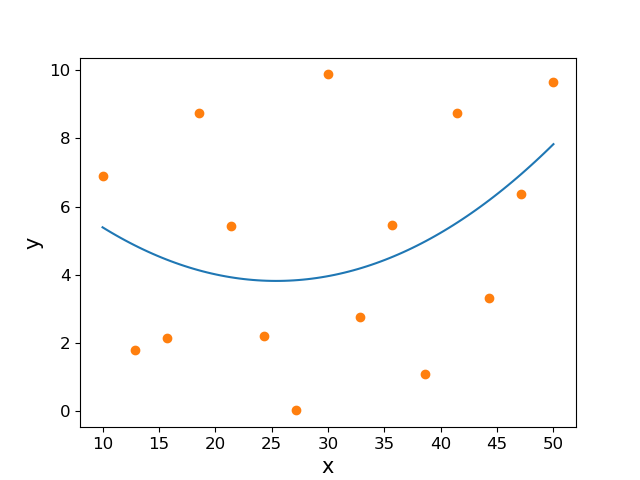
\includegraphics[width=\textwidth]{/Polynome/poly_deg2.png}
        \caption{Degree 2.}
        \label{fig:degree 2}
    \end{subfigure}
    \begin{subfigure}[b]{0.3\textwidth}
        \centering
        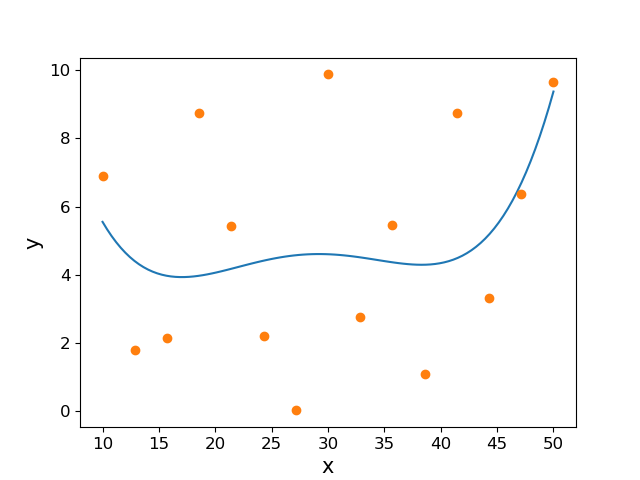
\includegraphics[width=\textwidth]{/Polynome/poly_deg4.png}
        \caption{Degree 4.}
        \label{fig:degree 4}
    \end{subfigure}
    \begin{subfigure}[b]{0.3\textwidth}
        \centering
        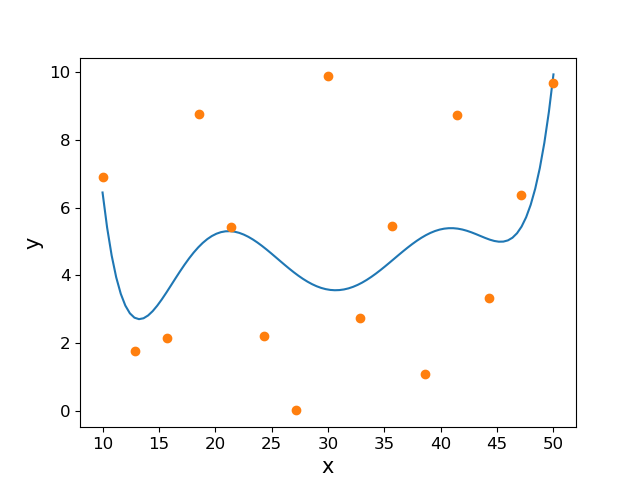
\includegraphics[width=\textwidth]{/Polynome/poly_deg6.png}
        \caption{Degree 6.}
        \label{fig:degree 6}
    \end{subfigure}
    \begin{subfigure}[b]{0.3\textwidth}
        \centering
        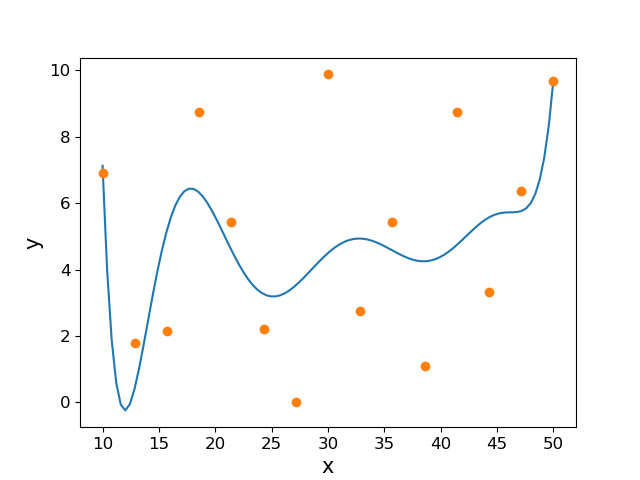
\includegraphics[width=\textwidth]{/Polynome/poly_deg8.png}
        \caption{Degree 8.}
        \label{fig:degree 8}
    \end{subfigure}
    \begin{subfigure}[b]{0.3\textwidth}
        \centering
        \includegraphics[width=\textwidth]{/Polynome/poly_deg10.png}
        \caption{Degree 10.}
        \label{fig:degree 10}
    \end{subfigure}
    \begin{subfigure}[b]{0.3\textwidth}
        \centering
        \includegraphics[width=\textwidth]{/Polynome/poly_deg12.png}
        \caption{Degree 12.}
        \label{fig:degree 12}
    \end{subfigure}
    \begin{subfigure}[b]{0.3\textwidth}
        \centering
        \includegraphics[width=\textwidth]{/Polynome/poly_deg14.png}
        \caption{Degree 14.}
        \label{fig:degree 14}
    \end{subfigure}
    \caption{Polynomial fitting of 15 points.} \label{fig:C7_poly}
\end{figure}

According to the theory, a polynomial of degree N can exactly fit N+1 points. However, polynomial of high order tends to fluctuate outside the domain defined by the set of points. On the set of Figures \ref{fig:C7_poly} are represented the fitting of a polynomial over 15 points for different degrees $d$.



As illustrated in the series of graphs, when the highest degree of the polynomial increases, the amplitude of the variations increases as well. More precisely, the magnitude at the extremity of the domain defined by the set of points is relatively large compared to the remaining of the function. Also, the increase of the magnitude can be observed on the ordinate. Indeed, the maximum value depicted on the axis goes from 10 for a degree $d=2$ too 700 for a degree $d=14$. Here, this increase of the scale occurs for a degree $d$ greater than 8.

Thus, it is required to minimize the degree of the polynomial to avoid these large fluctuations. This will be performed by  using the LS-R algorithm. The algorithm allows restricting the maximal degree of the polynomial while keeping a good accuracy at the given points. For the remaining of the report, the abbreviation LS-RP will refer to the least square regression algorithm using polynomials as basis functions.

\subsection{Splitting of the performance maps}
\quad\ When considering the performance maps of the compressor and the turbine, the range of value for the rotational speed can become quite large. However, if the domain to be extrapolated by the polynomial is too wide, an evident loss of accuracy will occur. 

To avoid this loss of accuracy, it would be interesting to split the maps before applying the least-squares regression algorithm. Therefore, the polynomial will be defined by parts. However, there isn't any guarantee that the value of the polynomial at the junction of two parts will be the same. To solve this issue, each part is partly superimposed on each other. Then, a linear blending is performed to remove the discontinuity between the different parts. 

Considering two functions $f_1(x,N)$ and $f_2(x,N)$ superimposed for value of $N\in [N_{start},N_{end}]$, the blended function $f_{1,2}(x,N)$ is defined as follows:
\begin{equation}
 f_{1,2}(x,N) = \begin{cases}
f_1(x,N) &\text{ if }N<N_{start}\\
f_1(x,N) + f_2(x,N) - f_1(x,N))\cdot \alpha &\text{ if } N\in [N_{start},N_{end}]\\
f_2(x,N) &\text{ if }N>N_{end}
\end{cases}   
\end{equation}
Where $\alpha$ is a coefficient for which its value is 0 for $N = N_{start}$ and 1 for $N = N_{end}$.  
\subsection{Compressor maps}
\quad\ The algorithm will first be applied on the compressor map. In the Brayton cycle code, the inlet condition of the compressor is specified. Thus, since the mass flow going through and the compressor rotational speed are known, the produced pressure ratio and the isentropic efficiency associated to the compression can be computed.

\subsubsection{Extrapolation of the map to low RPM}
\quad\, Before studying the polynomial fitting of the relations defining those operating variables, the extrapolation of the compressor performance map to the low rotational speed has to be described. Indeed, those operating points are not always calculated when the building of the map is performed. However, at these low rotational speeds, the flow starts to behave as an incompressible flow. Therefore, the method of extrapolation of the performance maps seen for the pumps in chapter \ref{C4} can be applied on the map.

As expressed in the chapter \ref{C4}, two similar operating points $A$ and $B$ are linked by the relations (\ref{eq:C7_mdot}) to (\ref{eq:C7_eta}). 

\begin{subequations}
\setstretch{1}
\begin{align}
    \dot{Q}_{c,B} &= \dot{Q}_{c,A} \cdot \frac{N_{corr,c,B}}{N_{corr,c,A}}\nonumber\\
    \dot{m}_{corr,c,B} &= \dot{m}_{corr,c,A} \cdot \frac{N_{corr,c,B}}{N_{corr,c,A}}\label{eq:C7_mdot}\\
    \Delta h_{B}^0 &= \Delta h_{A}^0 \cdot \left(\frac{N_{corr,c,B}}{N_{corr,c,A}}\right)^2 \label{eq:C7_Dh}\\
    \eta_{is,c,B} &= \eta_{is,c,A} \label{eq:C7_eta}
\end{align}
\end{subequations}
With $\Delta h^0 = h_{2}^0 - h_{1}^0$, where the inlet and outlet states of the compressor are denoted \textbf{1} and \textbf{2}.

The extrapolation assumes that the gas used is air with constant
$c_p=1005$ J/kg$\cdot$K and $r = 287$ J/kg$\cdot$K. 

To initialize the method, the following reference conditions need to be defined:

\begin{itemize}
    \setstretch{1}
    \item $T_{0}^0 = 293.15$K
    \item $h_{0}^0 = 0$
    \item $r = 287$ J/kg$\cdot$ K
    \item $k = \frac{c_p - r}{c_p} = 1.4$
\end{itemize}
Then, considering the known operating point $A$, the variation of the enthalpy $\delta_{A}^0$ is obtained  using the relations seen in the section \ref{C3:Isen_eff} is used. The mathematical development is expressed in (\ref{eq:C7_DhA}), where the inlet condition $1$ of the compressor corresponds to the reference conditions specified above.

\begin{align}
\setstretch{1}
    T_{A,1}^0 = T_{0}^0 &\text{ and } h_{A,1}^0 = h_{0}^0\nonumber\\
    \frac{T_{A,2,is}^0}{T_{A,1}^0} &= \left(\Pi_{tt,c,A}\right)^{\frac{k-1}{k}}\nonumber\\
    T_{A,2}^0 &= T_{A,1}^0 + \frac{T_{A,2,is}^0 - T_{A,1}^0}{\eta_{is,c,A}}\label{eq:C7_DhA}\\
    h_{A,2}^0 &= h_{0}^0 + c_p\cdot (T_{A,2}^0 - T_{0}^0)\nonumber\\
    \Rightarrow \Delta h_A^0 &= h_{A,2}^0  - h_{A,1}^0\nonumber
\end{align}

Once the enthalpy variation $\Delta h_A^0$ is computed, the one for the similar operating point $B$ can be obtained from the relation (\ref{eq:C7_Dh}).

Then, the total to total pressure ratio produced by the compressor at the operating point $B$ by applying backward the relations of (\ref{eq:C7_DhA}). Therefore, the following development (\ref{eq:C7_DhB}) can be derived.

\begin{align}
\setstretch{1}
    T_{B,2}^0 = T_{0}^0 &\text{ and } h_{B,2}^0 = h_{0}^0\nonumber\\
    h_{B,2}^0 &= \Delta h_B^0 + h_{B,1}^0\nonumber\\
    T_{B,2}^0 &= \frac{h_{B,2}^0 - h_{0}^0}{c_p} + T_0^0\label{eq:C7_DhB}\\
    T_{B,2,is}^0 &= \left(T_{B,2}^0 - T_{B,1}^0\right)\cdot \eta_{is,c,B} + T_{B,1}^0\nonumber\\
    \Pi_{tt,c,B} &= \left(\frac{T_{B,2,is}^0}{T_{B,1}^0}\right)^{\frac{k}{k-1}}\nonumber
\end{align}

A part of the map extrapolated to the low rotational speed is included in the Table \ref{tab:C7_compmap_LRPM}. 
\begin{longtable}[c]{@{}cccc|cccc@{}}
\caption{Normalized compressor map (Low RPM)}
\label{tab:C7_compmap_LRPM}\\
\toprule
$\mathbf{\dot{m}_{corr,c}}$ & $\mathbf{\Pi_{tt,c}}$ & $\mathbf{N_{corr,c}}$ & $\mathbf{\eta_{is,c}}$ & $\mathbf{\dot{m}_{corr,c}}$ & $\mathbf{\Pi_{tt,c}}$ & $\mathbf{N_{corr,c}}$ & $\mathbf{\eta_{is,c}}$ \\* \midrule
\endfirsthead
%
\endhead
%
\bottomrule
\endfoot
%
\endlastfoot
%
0.074                            & 0.933                      & 0.200                 & 0.948                       & 0.298                            & 0.987                      & 0.800                 & 0.948                       \\
0.108                            & 0.933                      & 0.200                 & 0.972                       & 0.434                            & 0.979                      & 0.800                 & 0.972                       \\
0.140                            & 0.933                      & 0.200                 & 0.835                       & 0.558                            & 0.972                      & 0.800                 & 0.835                       \\
0.167                            & 0.932                      & 0.200                 & 0.557                       & 0.667                            & 0.967                      & 0.800                 & 0.557                       \\
0.061                            & 0.934                      & 0.200                 & 0.896                       & 0.242                            & 0.991                      & 0.800                 & 0.896                       \\
0.091                            & 0.933                      & 0.200                 & 1.000                       & 0.364                            & 0.984                      & 0.800                 & 1.000                       \\
0.117                            & 0.933                      & 0.200                 & 0.975                       & 0.468                            & 0.978                      & 0.800                 & 0.975                       \\
0.140                            & 0.933                      & 0.200                 & 0.877                       & 0.558                            & 0.973                      & 0.800                 & 0.877                       \\
0.149                            & 0.941                      & 0.400                 & 0.948                       & 0.447                            & 0.999                      & 1.000                 & 0.948                       \\
0.217                            & 0.940                      & 0.400                 & 0.972                       & 0.651                            & 0.991                      & 1.000                 & 0.972                       \\
0.279                            & 0.938                      & 0.400                 & 0.835                       & 0.837                            & 0.975                      & 1.000                 & 0.835                       \\
0.333                            & 0.935                      & 0.400                 & 0.557                       & 1.000                            & 0.957                      & 1.000                 & 0.557                       \\
0.121                            & 0.942                      & 0.400                 & 0.896                       & 0.363                            & 1.000                      & 1.000                 & 0.896                       \\
0.182                            & 0.941                      & 0.400                 & 1.000                       & 0.545                            & 0.999                      & 1.000                 & 1.000                       \\
0.234                            & 0.940                      & 0.400                 & 0.975                       & 0.702                            & 0.990                      & 1.000                 & 0.975                       \\
0.279                            & 0.938                      & 0.400                 & 0.877                       & 0.838                            & 0.979                      & 1.000                 & 0.877                       \\* \bottomrule
\end{longtable}
\subsubsection{Compression ratio $\Pi_{tt,c}$}
\quad\ Now that the compressor map is defined for the whole range of rotational speed, the study can be conducted. First, the relation defining the compression ratio is (\ref{eq:C7_Pratio}).

\begin{equation}
    \setstretch{1}
    \Pi_{tt,c}(\dot{m}_{corr,c},N_{corr,c}) \label{eq:C7_Pratio}
\end{equation}

Based on the set of operating points characterizing the performance map of the machine, the relation can be defined by a polynomial using the least square regression algorithm.

First, the minimal degree of the polynomial representing the relation has to be established. For each polynomial built using the LS-RP, the values of the objective function $\textbf{F}$ and of the $\chi^2$ functions are computed. 

These values have to respectively be minimal and maximal in order to minimize the error regarding to the set of points. The table \ref{tab:C7_regcomp} includes the results from the analysis of the data from the Tables \ref{tab:C7_compmap} and \ref{tab:C7_compmap_LRPM}. 

It has to be known that the coefficients $a_{i,j}$ characterizing the polynomial are different for the two sets of operating points. This is the consequence of the splitting of the performance map. 


\begin{longtable}[c]{@{}ccc|cc@{}}
\caption{$\Pi_{tt,c}(\dot{m}_{corr,c},N_{corr,c})$ - regression results }
\label{tab:C7_regcomp}\\
\toprule
\textit{\textbf{Polynomial}} & \multicolumn{2}{c|}{High RPM}  & \multicolumn{2}{c}{Low RPM}    \\* \midrule
\endfirsthead
%
\endhead
%
\bottomrule
\endfoot
%
\endlastfoot
%
\multicolumn{1}{c}{\textbf{Degree}}              & \multicolumn{1}{c}{$\mathbf{F}$} & \multicolumn{1}{c|}{$\mathbf{\chi^2}$} & \multicolumn{1}{c}{$\mathbf{F}$} & \multicolumn{1}{c}{$\mathbf{\chi^2}$} \\
\multicolumn{1}{c}{\textbf{1}}                   & 0.094      & 0.772             & 3.20E-04   & 0.966             \\
\multicolumn{1}{c}{\textbf{2}}                   & 0.046      & 0.889             & 1.62E-04   & 0.983             \\
\multicolumn{1}{c}{\textbf{3}}                   & 0.024      & 0.942             & 1.60E-05   & 0.998             \\
\multicolumn{1}{c}{\textbf{4}}                   & 0.013      & 0.970             & 6.81E-06   & 0.999             \\
\multicolumn{1}{c}{\textbf{5}}                   & 0.008      & 0.981             & 6.24E-06   & 0.999             \\
\multicolumn{1}{c}{\textbf{6}}                   & 0.008      & 0.982             & 5.54E-06   & 0.999             \\* \bottomrule
\end{longtable}


These results show that for a degree $d=4$, the error with respect to the given points start to be acceptable.  Considering the low RPM operating points, the polynomial built perfectly fit the data starting from a degree $d=4$. The graphic representation of the two polynomials is given in the Figures \ref{fig:C7_polycomp_P_HRPM} and \ref{fig:C7_polycomp_P_LRPM}.

\begin{figure}[H]
    \setstretch{1}
    \centering
    \begin{subfigure}[b]{0.4\textwidth}
        \centering
        \includegraphics[width=\textwidth]{/Comp_map/HRPM/calc_0_2_1_map.png}
        \caption{High rotational speed}
        \label{fig:C7_polycomp_P_HRPM}
    \end{subfigure}
    \begin{subfigure}[b]{0.4\textwidth}
        \centering
        \includegraphics[width=\textwidth]{/Comp_map/LRPM/calc_0_2_1_map.png}
        \caption{Low rotational speed}
        \label{fig:C7_polycomp_P_LRPM}
    \end{subfigure}
    \caption{Polynomial regression ($d=4$) - $\Pi_{tt,c}(\dot{m}_{corr,c},N_{corr,c})$} \label{fig:C7_polycomp_P}
\end{figure}

The Figure \ref{fig:C7_polycomp_P_LRPM} shows that the iso-rotational speed curves are relatively closed from one to the others. The quality of the overall extrapolation would be improved if the gap between these curves is wider. 

By applying a multiplication factor on the pressure ratio, it is possible to create an artificial increase of this gap. Here, the factor selected is the corrected rotational speed $N_{corr,c}$. Therefore, the new relation is $[\Pi_{tt,c}\cdot N_{corr,c}](\dot{m}_{corr,c},N_{corr,c})$. 

After having applied this multiplication factor, the parametric study has been performed again. The outputs have been written in the Table \ref{tab:C7_regcomp2}.

\begin{longtable}[c]{@{}ccc|cc@{}}
\caption{$[\Pi_{tt,c}\cdot N_{corr,c}](\dot{m}_{corr,c},N_{corr,c})$ - regression results }
\label{tab:C7_regcomp2}\\
\toprule
\textit{\textbf{Polynomial}} & \multicolumn{2}{c|}{High RPM}  & \multicolumn{2}{c}{Low RPM}    \\* \midrule
\endfirsthead
%
\endhead
%
\bottomrule
\endfoot
%
\endlastfoot
%
\multicolumn{1}{c}{\textbf{Degree}}              & \multicolumn{1}{c}{$\mathbf{F}$} & \multicolumn{1}{c|}{$\mathbf{\chi^2}$} & \multicolumn{1}{c}{$\mathbf{F}$} & \multicolumn{1}{c}{$\mathbf{\chi^2}$} \\
\multicolumn{1}{c}{\textbf{1}}                   & 0.089      & 0.843             & 5.70E-04   & 1.000             \\
\multicolumn{1}{c}{\textbf{2}}                   & 0.042      & 0.925             & 5.01E-05   & 1.000             \\
\multicolumn{1}{c}{\textbf{3}}                   & 0.021      & 0.962             & 1.22E-05   & 1.000             \\
\multicolumn{1}{c}{\textbf{4}}                   & 0.011      & 0.980             & 6.31E-06   & 1.000             \\
\multicolumn{1}{c}{\textbf{5}}                   & 0.007      & 0.987             & 5.91E-06   & 1.000             \\
\multicolumn{1}{c}{\textbf{6}}                   & 0.007      & 0.988             & 5.24E-06   & 1.000             \\* \bottomrule
\end{longtable}

Comparing the two Tables \ref{tab:C7_regcomp} and \ref{tab:C7_regcomp2} shows that, for a even degree, the residual function $\chi^2$ has a higher value. This implies that the accuracy of the polynomial is improved over the set of points. 

The degree $d=4$ remains the best choice based on the results of the study. Respectively, the Figures \ref{fig:C7_polycomp_PN_HRPM} and \ref{fig:C7_polycomp_PN_LRPM} depict the polynomial for the high and low rotational speed operating points.

\begin{figure}[H]
    \setstretch{1}
    \centering
    \begin{subfigure}[b]{0.4\textwidth}
        \centering
        \includegraphics[width=\textwidth]{/Comp_map/HRPM/calc_0_2_12_map.png}
        \caption{High rotational speed}
        \label{fig:C7_polycomp_PN_HRPM}
    \end{subfigure}
    \begin{subfigure}[b]{0.4\textwidth}
        \centering
        \includegraphics[width=\textwidth]{/Comp_map/LRPM/calc_0_2_12_map.png}
        \caption{Low rotational speed}
        \label{fig:C7_polycomp_PN_LRPM}
    \end{subfigure}
    \caption{Polynomial regression ($d=4$) - $[\Pi_{tt,c}\cdot N_{corr,c}](\dot{m}_{corr,c},N_{corr,c})$} \label{fig:C7_polycomp_PN}
\end{figure}

\subsubsection{Isentropic efficiency $\eta_{is,c}$}
\quad\ The second operating variable to be determined is the isentropic efficiency. The first relation to be considered is (\ref{eq:C7_etarel}), where the pressure ratio is already multiplied by the rotational speed.
\begin{equation}
    \setstretch{1}
    \eta_{is,c}(\Pi_{tt,c}\cdot N_{corr,c},N_{corr,c}) \label{eq:C7_etarel}
\end{equation}
Considering this relation, a similar study over the degree of the polynomial has been considered. The obtained results have been included in the Table \ref{tab:C7_regcomp3}.

\begin{longtable}[c]{@{}ccc|cc@{}}
\caption{$\eta_{is,c}(\Pi_{tt,c}\cdot N_{corr,c},N_{corr,c})$ - regression results}
\label{tab:C7_regcomp3}\\
\toprule
\textit{\textbf{Polynomial}} & \multicolumn{2}{c|}{High RPM}                        & \multicolumn{2}{c}{Low RPM}    \\* \midrule
\endfirsthead
%
\endhead
%
\bottomrule
\endfoot
%
\endlastfoot
%
\multicolumn{1}{c}{\textbf{Degree}}              & \multicolumn{1}{c}{$\mathbf{F}$} & \multicolumn{1}{c|}{$\mathbf{\chi^2}$} & \multicolumn{1}{c}{$\mathbf{F}$} & \multicolumn{1}{c}{$\mathbf{\chi^2}$} \\
\multicolumn{1}{c}{\textbf{1}}                   & 0.097      & 0.709             & 0.215      & 0.242             \\
\multicolumn{1}{c}{\textbf{2}}                   & 0.024      & 0.929             & 0.187      & 0.342             \\
\multicolumn{1}{c}{\textbf{3}}                   & 0.005      & 0.986             & 0.086      & 0.698             \\
\multicolumn{1}{c}{\textbf{4}}                   & 0.004      & 0.988            & 0.030      & 0.896             \\
\multicolumn{1}{c}{\textbf{5}}                   & 0.002      & 0.993           & 0.030      & 0.894             \\
\multicolumn{1}{c}{\textbf{6}}                   & 0.002      & 0.994                                  & 0.030      & 0.893             \\* \bottomrule
\end{longtable}

The results expressed in the Table \ref{tab:C7_regcomp3} show that, the fitting function has difficulties to represent the relation for the low rotational speed operating point. 

The reason behind is that the pressure ratio does not vary much on a given iso-rotational speed curve. Therefore, as depicted in the Figure \ref{fig:C7_polycomp_eta1_LRPM}, the polynomial has a really high slope.  

\begin{figure}[H]
    \setstretch{1}
    \centering
    \begin{subfigure}[b]{0.4\textwidth}
        \centering
        \includegraphics[width=\textwidth]{/Comp_map/HRPM/calc_12_2_3_map.png}
        \caption{High rotational speed}
        \label{fig:C7_polycomp_eta1_HRPM}
    \end{subfigure}
    \begin{subfigure}[b]{0.4\textwidth}
        \centering
        \includegraphics[width=\textwidth]{/Comp_map/LRPM/calc_12_2_3_map.png}
        \caption{Low rotational speed}
        \label{fig:C7_polycomp_eta1_LRPM}
    \end{subfigure}
    \caption{Polynomial regression ($d=3$) - $\eta_{is,c}(\Pi_{tt,c}\cdot N_{corr,c},N_{corr,c})$} \label{fig:C7_polycomp_eta1}
\end{figure}

However, for the high rotational speed operating points, the variation of the pressure ratio is large enough to provide a reliable polynomial regression. 

This relation will only be used for the high rotational speeds. Thus for these operating points, a degree $d=3$ will be selected since the accuracy does not improve significantly beyond for $d>3$.

Considering the inverse relation $[\Pi_{tt,c}\cdot N_{corr,c}](\eta_{is,c},N_{corr,c})$ instead will transpose the graph. Using this tweak will make horizontal the iso-rotational speed curves for the low rotational speed operating points. The results from the parametric study for this part of the compressor map are given in Table \ref{tab:C7_regcomp5}. 


\begin{longtable}[c]{@{}ccc@{}}
\caption{$[\Pi_{tt,c}\cdot N_{corr,c}](\eta_{is,c},N_{corr,c})$ - regression results }
\label{tab:C7_regcomp5}\\
\toprule
\textit{\textbf{Polynomial}} & &  \\* \midrule
\endfirsthead
%
\endhead
%
\bottomrule
\endfoot
%
\endlastfoot
%
\multicolumn{1}{c}{\textbf{Degree}}              & \multicolumn{1}{c}{$\mathbf{F}$}            & \multicolumn{1}{c}{$\mathbf{\chi^2}$}                  \\
\multicolumn{1}{c}{\textbf{1}}                   & 9.18E-04   & 0.999             \\
\multicolumn{1}{c}{\textbf{2}}                   & 4.16E-04   & 1.000             \\
\multicolumn{1}{c}{\textbf{3}}                   & 2.32E-04   & 1.000             \\
\multicolumn{1}{c}{\textbf{4}}                   & 1.79E-04   & 1.000             \\
\multicolumn{1}{c}{\textbf{5}}                   & 1.48E-04   & 1.000             \\
\multicolumn{1}{c}{\textbf{6}}                   & 7.87E-05   & 1.000             \\* \bottomrule
\end{longtable}
Here, the regression of the points is nearly perfect considering any value of the polynomial degree $d$. To avoid the generation of a polynomial with potentially high variations, the degree $d=3$ has been selected for this relation.

The Figure \ref{fig:C7_polycomp_eta3_LRPM} depicts the relation for the low rotational speed operating points.

\begin{figure}[H]
    \centering
    \includegraphics[width=0.4\textwidth]{/Comp_map/LRPM/calc_3_2_12_map.png}
    \caption{Polynomial regression ($d=3$) - $[\Pi_{tt,c}\cdot N_{corr,c}](\eta_{is,c},N_{corr,c})$}
    \label{fig:C7_polycomp_eta3_LRPM}
\end{figure}
    
When increasing the natural value (in RPM) of $N_{corr,c}$, the relation $\eta_{is,c}(\Pi_{tt,c}\cdot N_{corr,c},N_{corr,c})$ obtained by polynomial regression becomes accurate enough to be used instead. 

As a summary, the Table \ref{tab:C7_compmaprel} includes the results of the parametric studies for the retained degree of each relation. 

\begin{longtable}[c]{@{}cccc|cc@{}}
\caption{Compressor map - Table of relations}
\label{tab:C7_compmaprel}\\
\toprule
\multicolumn{1}{c}{\multirow{2}{*}{\textbf{Relation}}} & \multicolumn{1}{c}{\multirow{2}{*}{\textbf{Degree}}} & \multicolumn{2}{c|}{High RPM}                  & \multicolumn{2}{c}{Low RPM}                   \\
\multicolumn{1}{c}{}                                            & \multicolumn{1}{c}{}                        & \multicolumn{1}{c}{$\mathbf{F}$}          & \multicolumn{1}{c|}{$\chi^2$}               & \multicolumn{1}{c}{$\mathbf{F}$}          & \multicolumn{1}{c}{$\chi^2$}               \\* \midrule
\endfirsthead
%
\endhead
%
\bottomrule
\endfoot
%
\endlastfoot
%
$[\Pi_{tt,c}\cdot N_{corr,c}](\dot{m}_{corr,c},N_{corr,c})$                   & \multicolumn{1}{c}{\textbf{4}}                                           & 0.011
                 & 0.980
                  & 6.31E-06
      & 1.000                 \\
$\eta_{is,c}(\Pi_{tt,c}\cdot N_{corr,c},N_{corr,c})$                          & \multicolumn{1}{c}{\textbf{3}}                                           & 0.005             & 0.986                  & \multicolumn{1}{c}{-} & \multicolumn{1}{c}{-} \\
$[\Pi_{tt,c}\cdot N_{corr,c}](\eta_{is,c},N_{corr,c})$                        & \multicolumn{1}{c}{\textbf{3}}                                           & \multicolumn{1}{c}{-} & \multicolumn{1}{c|}{-} & 2.32E-04              & 1.000                 \\* \bottomrule
\end{longtable}

\subsubsection{N-1 study}
\quad\ The degree of the polynomial has been selected based on the quality of the regression of the set of operating points. For each relation, the LS-RP has been applied to determine the best degree.

Now that the degree of the polynomials has been set, the N-1 study can be performed. This study consists in comparing the error on a given operating point $i$ when the polynomial is built using the data where this operating point $i$ has been removed. For the nomenclature, the polynomial obtained considering the complete data is noted $f_N(x,y)$, and the one obtained for the data where the operating point $i$ is missing will be noted $f_i(x,y)$.

Considering the relations in the Table \ref{tab:C7_compmaprel}, three different types of error have been computed for each operating point $i$:

\begin{itemize}
    \setstretch{1}
    \item $\Delta z_{i,N}$: Error, in percent, on the polynomial $f_i\left(x(i),y(i)\right)$ value compared with the value of $f_N\left(x(i),y(i)\right)$.
    \item $\Delta z_{N,ref}$: Error, in percent, on the polynomial $f_N\left(x(i),y(i)\right)$ value compared with the actual value of the relation for the operating point $\left(x(i),y(i)\right)$.
    \item $\Delta z_{i,ref}$: Error, in percent, on the polynomial $f_i\left(x(i),y(i)\right)$ value compared with the actual value of the relation for the operating point $\left(x(i),y(i)\right)$.
\end{itemize}

The mean and maximal errors for each relation are included in the Table \ref{tab:C7_Nm1}. The results for each operating point $i$ are given in the annex \ref{ann_Nm1}.

\begin{longtable}[c]{@{}lclcl|clcl@{}}
\caption{N-1 study - error of accuracy}
\label{tab:C7_Nm1}\\
\toprule
\multicolumn{1}{c}{\multirow{3}{*}{Relation}} & \multicolumn{4}{c|}{$\Delta z_{i,N}$ (\%)}                                                                  & \multicolumn{4}{c}{$\Delta z_{N,ref}$ (\%)}                                                                   \\
\multicolumn{1}{c}{}                          & \multicolumn{2}{c}{High RPM}                         & \multicolumn{2}{c|}{Low RPM}                         & \multicolumn{2}{c}{High RPM}                          & \multicolumn{2}{c}{Low RPM}                           \\
\multicolumn{1}{c}{}                          & Mean                       & \multicolumn{1}{c}{Max} & Mean                      & \multicolumn{1}{c|}{Max} & Mean                        & \multicolumn{1}{c}{Max} & Mean                        & \multicolumn{1}{c}{Max} \\* \midrule
\endfirsthead
%
\endhead
%
\bottomrule
\endfoot
%
\endlastfoot
%
$[\Pi N_{tt,c}](\dot{m}_{corr,c},N_{corr,c})$ & \multicolumn{1}{l}{5.850}  & 60.428                  & \multicolumn{1}{l}{0.138} & 2.124                    & \multicolumn{1}{l}{4.161}   & 12.456                  & \multicolumn{1}{l}{0.065}   & 0.191                   \\
$\eta_{is,c}(\Pi N_{tt,c},N_{corr,c})$        & \multicolumn{1}{l}{1.098}  & 5.799                   & \multicolumn{2}{c|}{-}                               & \multicolumn{1}{l}{1.537}   & 7.015                   & \multicolumn{2}{c}{-}                                 \\
$[\Pi N_{tt,c}](\eta_{is,c},N_{corr,c})$      & \multicolumn{2}{c}{-}                                & \multicolumn{1}{l}{0.429} & 5.304                    & \multicolumn{2}{c}{-}                                 & \multicolumn{1}{l}{0.514}   & 1.229                   \\* \midrule
\multicolumn{1}{c}{\multirow{3}{*}{Relation}} & \multicolumn{4}{c|}{$\Delta z_{i,ref}$ (\%)}                                                                & \multicolumn{4}{c}{$\Delta \left(\Delta z_{i,ref}, \Delta z_{N,ref}\right)$ (\%)}                             \\
\multicolumn{1}{c}{}                          & \multicolumn{2}{c}{High RPM}                         & \multicolumn{2}{c|}{Low RPM}                         & \multicolumn{2}{c}{High RPM}                          & \multicolumn{2}{c}{Low RPM}                           \\
\multicolumn{1}{c}{}                          & Mean                       & \multicolumn{1}{c}{Max} & Mean                      & \multicolumn{1}{c|}{Max} & Mean                        & \multicolumn{1}{c}{Max} & Mean                        & \multicolumn{1}{c}{Max} \\* \midrule
$[\Pi N_{tt,c}](\dot{m}_{corr,c},N_{corr,c})$ & \multicolumn{1}{l}{10.081} & 61.323                  & \multicolumn{1}{l}{0.204} & 2.125                    & \multicolumn{1}{l}{142.259} & 392.331                 & \multicolumn{1}{l}{209.371} & 1013.865                \\
$\eta_{is,c}(\Pi N_{tt,c},N_{corr,c})$        & \multicolumn{1}{l}{2.637}  & 9.760                   & \multicolumn{2}{c|}{-}                               & \multicolumn{1}{l}{71.490}  & 39.124                  & \multicolumn{2}{c}{-}                                 \\
$[\Pi N_{tt,c}](\eta_{is,c},N_{corr,c})$      & \multicolumn{2}{c}{-}                                & \multicolumn{1}{l}{0.942} & 5.998                    & \multicolumn{2}{c}{-}                                 & \multicolumn{1}{l}{83.270}  & 388.002                 \\* \bottomrule
\end{longtable}
With $\Pi N_{tt,c} = \Pi_{tt,c}\cdot N_{corr,c}$.

Multiple comments can be made based on these results. First, considering the increase of the errors going from $f_N(x,y)$ to $f_i(x,y)$, it can be noticed that the polynomial is more sensitive to the removal of one operating point when considering the operating points at low rotational speed.

Indeed, for the relation $[\Pi_{tt,c}\cdot N_{corr,c}](\dot{m}_{corr,c},N_{corr,c})$, the maximal increase of the error goes from around 400\% for the high RPM rotational speed to 1000\% for the low rotational speed operating points.

However, in absolute value the error at low rotational speed is much smaller. This is due to the close proximity of the different points on each iso-rotational speed curve. Thus, the polynomial is nearly a straight line for each of these curves. 

The impact on the accuracy of the polynomial when removing a point depends on the location of the point on the associated iso-curve. Indeed, from the results in the annex \ref{ann_Nm1} it can be observed that for the points located at the extremity of the curves, the error $\Delta z_{i,N}$ (\%) isn't very large if one of these points is removed.

However, if one operating point at the extremity is removed, the error $\Delta z_{i,N}$ (\%) becomes non-negligible. When removing an extremity point, the polynomial has to perform an extrapolation of the set of points to compute the value of the relation at this point. 

While the interpolation between is relatively accurate, the extrapolation really depends on the quality of the fitting function. The extrapolation is often valid for the points close to the first or last point defining the curve. This observation justified the motivation to extrapolate to the low rotational speeds before building the polynomial. Without this extrapolation using the similarity equations of used for the pumps, the compressor map would be unusable at low rotational speed. 

\subsection{Delimitation of the compressor map domain}
\quad\ When studying the compressor, for each rotational speed the range of operating points is bounded by a minimal and maximal mass flow rate. The two respectively correspond to the surge and the choke limits described in the chapter \ref{C4}. The purpose of this section is to express several numerical methods to estimate these boundary limits.

\subsubsection{Triangulation without constraints}
\quad\ The first method consisted in creating a triangular mesh not constraint through the couple of points $(\dot{m}_{corr,c},\Pi_{tt,c})$. This method has some advantages with first the rapidity of the method. Indeed, it does not take lots of computer resources to generate the mesh. Also, once the triangles created, the algorithm to check if the operating point is inside or outside the domain is really easy.

However, there are serious flaws that make the method unusable for the targeted application. Indeed, while the method gives easy tools to reject or not an operating point, finding the coordinates $(\dot{m}_{corr,c},\Pi_{tt,c})$ of the boundary for a given rotational speed is more difficult. 

The other weakness of the triangulation method is that it only works well with convex hull. The reason behind is that during the triangulation process, the program building the triangle does not know how the points are linked together. Unfortunately, some sections of the compressor map are not convex but concave. Therefore, when performing the triangulation, the concavity \textit{disappears} and the resulting mesh exceeds the real envelope of the map.


\begin{figure}[h]
    \centering
    \includegraphics[width=0.5\textwidth]{/Comp_map/map_triang.png}
    \caption{Simple triangulation of the compressor map}
    \label{fig:C7_trimap}
\end{figure}

Figure \ref{fig:C7_trimap} depicts the results of the triangulation of the compressor map. In red is represented the compressor map boundary, and in green is represented the mesh.

As it can be seen on the graph, the surge line is misrepresented by the mesh. The limit provided by the triangulation is very optimistic and doesn't correspond with the reality. 

\subsubsection{Triangulation with constraints}
\quad\ As explained in last lines, the basic triangulation method cannot handle concave hull by itself. In order to take into consideration these shapes, some conditions have to be set to reject or not the triangle of the mesh. A selection algorithm  has been developed \cite{Dwyer2014} based on the geometry of the triangle.

To illustrate the algorithm, the triangle with its circumscribed circle on Figure \ref{fig:C7_triangmesh} can be considered.

\begin{figure}[h]
    \centering
    \includegraphics[width=0.4\textwidth]{Comp_map/triang_mesh.png}
    \caption{Triangle with its coordinates within the mesh}
    \label{fig:C7_triangmesh}
\end{figure}

The three nodes $i_a$, $i_b$ and $i_c$ are respectively characterized by the coordinates $(x_a,y_a)$, $(x_b,y_b)$, $(x_c,y_c)$. Using the coordinates, the length of the triangle edges are computed as follows.

\begin{align*}
    \setstretch{1}
    l_a &= \sqrt{(x_a - x_b)^2 + (y_a - y_b)^2}\\
    l_b &= \sqrt{(x_b - x_c)^2 + (y_b - y_c)^2}\\
    l_c &= \sqrt{(x_c - x_a)^2 + (y_c - y_a)^2}
\end{align*}
Then, the intermediary quantity $s$, called semi-perimeter, is computed using the formula (\ref{eq:C7_semiperim}).

\begin{equation}
    \setstretch{1}
    s = \frac{a + b + c}{2}\label{eq:C7_semiperim}
\end{equation}
Using $l_a$, $l_b$, $l_c$, and $s$, the radius $circ_R$ of the circumscribed circle can be calculated using the relation (\ref{eq:C7_circum}). 

\begin{equation}
    \setstretch{1}
   circ_r = \frac{a\cdot b\cdot c}{4\cdot \sqrt{s\cdot (s - l_a)\cdot (s - l_b)\cdot (s - l_c)}}\label{eq:C7_circum}
\end{equation}

Now that the radius of the circumscribed circle of the triangle has been computed, the triangle will be rejected if the condition $circ_r <\frac{1}{\alpha}$ is not satisfied. This condition is justified by noting that for triangles outside the envelope, the radius will likely be bigger since all these external triangles has one obtuse angle. The parameter $\alpha$ needs to be tuned in order to eliminate the triangles outside the concave hull. 

The series of Figures \ref{fig:C7_alpha} illustrates the triangle mesh considering different values for the parameter $\alpha$.

\begin{figure}[h]
    \setstretch{1}
    \centering
    \begin{subfigure}[b]{0.3\textwidth}
        \centering
        \includegraphics[width=\textwidth]{/alpha/map_triang0_0.png}
        \caption{$\alpha=0$.}
        \label{fig:alpha0}
    \end{subfigure}
    \begin{subfigure}[b]{0.3\textwidth}
        \centering
        \includegraphics[width=\textwidth]{/alpha/map_triang1_0.png}
        \caption{$\alpha=1$.}
        \label{fig:alpha1}
    \end{subfigure}
    \begin{subfigure}[b]{0.3\textwidth}
        \centering
        \includegraphics[width=\textwidth]{/alpha/map_triang2_0.png}
        \caption{$\alpha=2$.}
        \label{fig:alpha2}
    \end{subfigure}
    \begin{subfigure}[b]{0.3\textwidth}
        \centering
        \includegraphics[width=\textwidth]{/alpha/map_triang3_0.png}
        \caption{$\alpha=3$.}
        \label{fig:alpha3}
    \end{subfigure}
    \begin{subfigure}[b]{0.3\textwidth}
        \centering
        \includegraphics[width=\textwidth]{/alpha/map_triang4_0.png}
        \caption{$\alpha=4$.}
        \label{fig:alpha4}
    \end{subfigure}
    \begin{subfigure}[b]{0.3\textwidth}
        \centering
        \includegraphics[width=\textwidth]{/alpha/map_triang5_0.png}
        \caption{$\alpha=5$.}
        \label{fig:alpha5}
    \end{subfigure}
    \begin{subfigure}[b]{0.3\textwidth}
        \centering
        \includegraphics[width=\textwidth]{/alpha/map_triang6_0.png}
        \caption{$\alpha=6$.}
        \label{fig:alpha6}
    \end{subfigure}
    \begin{subfigure}[b]{0.3\textwidth}
        \centering
        \includegraphics[width=\textwidth]{/alpha/map_triang7_0.png}
        \caption{$\alpha=7$.}
        \label{fig:alpha7}
    \end{subfigure}
    \begin{subfigure}[b]{0.3\textwidth}
        \centering
        \includegraphics[width=\textwidth]{/alpha/map_triang8_0.png}
        \caption{$\alpha=8$.}
        \label{fig:alpha8}
    \end{subfigure}
    \caption{Triangulation with triangle selection condition.} \label{fig:C7_alpha}
\end{figure}

The picture \ref{fig:alpha3} shows that for $\alpha=3$, most of the triangles outside the map domain are rejected. However, for the low pressure ratio it still remains some non-desired artifacts. Increasing the value of the parameter $\alpha$ would allow rejecting these
triangles as well but, some triangles within the domain also start to be removed. So, the value $\alpha=3$ is a good compromise.

\subsubsection{2D level-set}
\quad\ The triangulation with a condition to select the triangles provides relatively good results. However, this method is not really robust because each time a new map is provided to the program, the value of the parameter $\alpha$ has to be tuned by hand. An automatic method would consist in defining a level-set function that would delimit the performance map domain.

First has been considered a 2 dimensional function defined by the coordinates $(\dot{m}_{corr,c},\Pi_{tt,c})$ of the boundary points of the map. To build this function, a linear interpolation between these points have been used. Linear interpolation is chosen to have an interpolated surge line that is more restrictive than the actual surge line.

On Figure \ref{fig:C7_LS2D} is represented the level set function.

\begin{figure}[h]
    \centering
    \includegraphics[width=0.5\textwidth]{Comp_map/2D_LS.png}
    \caption{2D level-set function.}
    \label{fig:C7_LS2D}
\end{figure}

Compared to the triangulation, the computation of the boundary coordinates for a given rotational speed $N_c$ can easily be found by determining the intersection points between the level-set function $f_{ls,2D}$ and the interpolation function $\Pi_{tt,c}(\dot{m}_{corr,c},N_{corr,c})$. 
However, this 2D level-set function needs to be defined by parts since for some value of mass flow rate $\dot{m}_{corr,c}$, there exist two corresponding values for the pressure ratio $\Pi_{tt,c}$. Also, the data need to be pre-processed to only retained the boundary points of the maps. 

\subsubsection{3D level-set}
\quad\ The two cons of the 2D level-set can be erased by considering a 3D level-set. Here, the principle then to be closed to the performance maps regressions described in the previous parts of this section. However, here what is desired is a function defined inside the cloud of points and equal to the NULL value outside the cloud. 



\begin{figure}[H]
    \centering
    \includegraphics[width=0.5\textwidth]{Comp_map/3D_LS.png}
    \caption{3D level-set function - color bar representing the value of the pressure ratio.}
    \label{fig:C7_LS3D}
\end{figure}
The relation used to build the 3D level-set function $f_{ls,3D}$ is $\dot{m}_{corr,c} = \dot{m}_{corr,c}(\Pi_{tt,c},N_{corr,c})$. On Figure \ref{fig:C7_LS3D} is illustrated this level-set function. 
For each corrected rotational speed $N_{corr,c}c$, the function gives all the admissible couples $(\dot{m}_{corr,c},\Pi_{tt,c})$ based on the compressor map initially provided. 

Considering first the surge line, the limit drawn by the function is relatively close to the expected surge. If some margin is applied, the surge line can be nicely characterized by this 3D level-set function. 

\subsection{Estimation of the choke line}
\quad\ The choke lines can be defined by the 3D level-set function as well but, an alternative solution using the least square regression algorithm can be considered.


In chapter \ref{C4}, it has been explained that the relation $\Pi_{tt,c}(\dot{m}_{corr,c},N_{corr,c})$ is characterized by an infinite slope when the compressor is choking. However, polynomials are not designed to represent infinite slopes in for abscissa different from the infinity.

Considering the inverse relation $\dot{m}_{corr,c}(\Pi_{tt,c},N_{corr,c})$, the choke limit will happen when the derivative of the function is equal to zeros. Instead of considering this relation as it is, the pressure ratio can be multiplied by the rotational speed $N_{corr,c}$. After the parametric study on the polynomial degree $d$, the results obtained have been written in the Table \ref{tab:C7_regcomp4}.

\begin{longtable}[c]{@{}ccc|cc@{}}
\caption{$\dot{m}_{corr,c}(\Pi_{tt,c}\cdot N_{corr,c},N_{corr,c})$ - regression results}
\label{tab:C7_regcomp4}\\
\toprule
\textit{\textbf{Polynomial}} & \multicolumn{2}{c|}{High RPM}  & \multicolumn{2}{c}{Low RPM}    \\* \midrule
\endfirsthead
%
\endhead
%
\bottomrule
\endfoot
%
\endlastfoot
%
\textbf{Degree}              & \multicolumn{1}{c}{$\mathbf{F}$} & \multicolumn{1}{c|}{$\mathbf{\chi^2}$} & \multicolumn{1}{c}{$\mathbf{F}$} & \multicolumn{1}{c}{$\mathbf{\chi^2}$} \\
\textbf{1}                   & 0.103      & 0.618             & 0.130      & 0.865             \\
\textbf{2}                   & 0.037      & 0.863             & 0.033      & 0.966             \\
\textbf{3}                   & 0.016      & 0.940             & 0.011      & 0.989             \\
\textbf{4}                   & 0.012      & 0.955             & 0.008      & 0.992             \\
\textbf{5}                   & 0.011      & 0.961             & 0.008      & 0.992             \\
\textbf{6}                   & 0.010      & 0.962             & 0.008      & 0.992             \\* \bottomrule
\end{longtable}

As for the other relation, the accuracy provided by a polynomial of degree $d=3$ is already very acceptable. The polynomials obtained for the two maps \ref{tab:C7_compmap} and \ref{tab:C7_compmap_LRPM} are depicted in the set of Figure \ref{fig:C7_polycomp_m}.

\begin{figure}[H]
    \setstretch{1}
    \centering
    \begin{subfigure}[b]{0.4\textwidth}
        \centering
        \includegraphics[width=\textwidth]{/Comp_map/HRPM/calc_12_2_0_map.png}
        \caption{High rotational speed}
        \label{fig:C7_polycomp_m_HRPM}
    \end{subfigure}
    \begin{subfigure}[b]{0.4\textwidth}
        \centering
        \includegraphics[width=\textwidth]{/Comp_map/LRPM/calc_12_2_0_map.png}
        \caption{Low rotational speed}
        \label{fig:C7_polycomp_m_LRPM}
    \end{subfigure}
    \caption{Polynomial regression ($d=3$) - $\dot{m}_{corr,c}(\Pi_{tt,c}\cdot N_{corr,c},N_{corr,c})$} \label{fig:C7_polycomp_m}
\end{figure}

Considering first the map related to the high rotational speed operating points, it can be noticed that the derivative of the iso-curves can be at most two-time equal to zeros in the domain of validity of the map. Since the value that is interesting is the maximal mass flow rate, the mass flow rate at the local maximum is the value that will characterize the choke line.


This method works well with the high rotational speed operating points. However, for the low rotational speed operating points, the iso-rotational speed curves are quasi-vertical, making difficult the regression. Also, the local minimum and maximum are really far from the boundary of the compressor map.

Thus, in the event that there is no operating point for which the derivative is equal to zeros, the maximal mass flow rate will be the one such that the compression ratio produced by the compressor is equal to one.


\subsection{Turbine maps}
\quad\ From now, only the compressor maps have been considered. However, the extrapolation of the turbine maps using a fitting function is also required in order to characterize the turbine operating point. In the beginning of the current section, it was said that the two relations that need to be obtained are (\ref{eq:C7_turbMCbis}) and (\ref{eq:C7_turbETAbis}).

\begin{subequations}
\setstretch{1}
\begin{equation}
    \dot{m}_{corr,t}(\Pi_{tt,t},N_{corr,t})\label{eq:C7_turbMCbis}
\end{equation}
\begin{equation}
    \eta_{is,t}(\Pi_{tt,t},N_{corr,t})\label{eq:C7_turbETAbis}
\end{equation}
\end{subequations}

Based on what has been observed when constructing the polynomial for the compressor map, it is preferable to multiply the pressure ratio by the rotational speed within the relation.

Thus, instead of considering the relations (\ref{eq:C7_turbMCbis}) and (\ref{eq:C7_turbETAbis}), the relations (\ref{eq:C7_turbMCbis2}) and (\ref{eq:C7_turbETAbis2}) will be considered for the building of the polynomials.


\begin{subequations}
\setstretch{1}
\begin{equation}
    \dot{m}_{corr,t}(\Pi_{tt,t}\cdot N_{corr,t},N_{corr,t})\label{eq:C7_turbMCbis2}
\end{equation}
\begin{equation}
    \eta_{is,t}(\Pi_{tt,t}\cdot N_{corr,t},N_{corr,t})\label{eq:C7_turbETAbis2}
\end{equation}
\end{subequations}

Using the least square regression algorithm, a parametric study on the degree of the polynomial has conducted. The set of operating points considered is the one included in the Table \ref{tab:C7_turbmap}. 

\begin{longtable}[c]{@{}cccc|cccc@{}}
\caption{Normalized turbine map}
\label{tab:C7_turbmap}\\
\toprule
$\mathbf{\dot{m}_{corr,t}}$ & $\mathbf{\Pi_{tt,t}}$ & $\mathbf{N_{corr,t}}$ & $\mathbf{\eta_{is,t}}$ & $\mathbf{\dot{m}_{corr,t}}$ & $\mathbf{\Pi_{tt,t}}$ & $\mathbf{N_{corr,t}}$ & $\mathbf{\eta_{is,t}}$ \\* \midrule
\endfirsthead
%
\endhead
%
\bottomrule
\endfoot
%
\endlastfoot
%
0.620                            & 0.342                      & 0.692                 & 0.913                       & 0.945                            & 0.618                      & 0.846                 & 0.955                       \\
0.768                            & 0.392                      & 0.692                 & 0.960                       & 0.959                            & 0.660                      & 0.846                 & 0.950                       \\
0.817                            & 0.424                      & 0.692                 & 0.936                       & 0.979                            & 0.746                      & 0.846                 & 0.939                       \\
0.857                            & 0.457                      & 0.692                 & 0.921                       & 0.985                            & 0.792                      & 0.846                 & 0.933                       \\
0.892                            & 0.491                      & 0.692                 & 0.910                       & 0.997                            & 0.933                      & 0.846                 & 0.923                       \\
0.957                            & 0.605                      & 0.692                 & 0.876                       & 0.580                            & 0.364                      & 1.000                 & 0.582                       \\
0.969                            & 0.646                      & 0.692                 & 0.866                       & 0.723                            & 0.416                      & 1.000                 & 0.834                       \\
0.986                            & 0.732                      & 0.692                 & 0.850                       & 0.782                            & 0.445                      & 1.000                 & 0.933                       \\
0.992                            & 0.777                      & 0.692                 & 0.844                       & 0.827                            & 0.478                      & 1.000                 & 0.975                       \\
1.000                            & 0.915                      & 0.692                 & 0.821                       & 0.862                            & 0.513                      & 1.000                 & 0.990                       \\
0.597                            & 0.351                      & 0.846                 & 0.740                       & 0.932                            & 0.631                      & 1.000                 & 1.000                       \\
0.750                            & 0.402                      & 0.846                 & 0.963                       & 0.947                            & 0.673                      & 1.000                 & 0.999                       \\
0.805                            & 0.432                      & 0.846                 & 0.977                       & 0.968                            & 0.762                      & 1.000                 & 0.996                       \\
0.847                            & 0.465                      & 0.846                 & 0.981                       & 0.976                            & 0.807                      & 1.000                 & 0.994                       \\
0.881                            & 0.500                      & 0.846                 & 0.977                       & 0.993                            & 1.000                      & 1.000                 & 0.988                       \\* \bottomrule
\end{longtable}

After applying the LS-RP on the above data for the two relations, the results obtained have been written into the Table \ref{tab:reg_turbmap1}. 
\begin{longtable}[c]{@{}ccc|cc@{}}
\caption{Regression results - Turbine map}
\label{tab:reg_turbmap1}\\
\toprule
\textit{\textbf{Polynomial}} & \multicolumn{2}{c|}{$\dot{m}_{corr,t}(\Pi_{tt,t}\cdot N_{corr,t},N_{corr,t})$} & \multicolumn{2}{c}{$\eta_{is,t}(\Pi_{tt,t}\cdot N_{corr,t},N_{corr,t})$} \\* \midrule
\endfirsthead
%
\endhead
%
\bottomrule
\endfoot
%
\endlastfoot
%
\textbf{Degree}              & \multicolumn{1}{c}{$\mathbf{F}$}                  & \multicolumn{1}{c|}{$\mathbf{\chi^2}$}                 & \multicolumn{1}{c}{$\mathbf{F}$}               & \multicolumn{1}{c}{$\mathbf{\chi^2}$}               \\
\textbf{1}                   & 0.044                       & 0.768                             & 0.103                    & 0.111                           \\
\textbf{2}                   & 0.011                       & 0.941                             & 0.045                    & 0.608                           \\
\textbf{3}                   & 1.97E-03                    & 0.990                             & 0.013                    & 0.887                           \\
\textbf{4}                   & 3.01E-04                    & 0.998                             & 3.94E-03                 & 0.966                           \\
\textbf{5}                   & 6.49E-05                    & 1.000                             & 1.70E-03                 & 0.985                           \\
\textbf{6}                   & 1.66E-05                    & 1.000                             & 6.23E-04                 & 0.995                           \\* \bottomrule
\end{longtable}

\subsubsection{Corrected mass flow rate $\dot{m}_{corr,t}$}
\quad\ For the first relation, the value of the $\chi^2$ and of the objective function $F$ shows that the polynomial fits quasi-perfectly the set of points for a degree $d \geq 3$ of the polynomial. However, an improvement can be by multiplying in the first relation the corrected mass flow rate $\dot{m}_{corr,t}$ by the pressure ratio.

To illustrate the improvement, the Figures \ref{fig:C7_mturb3} and \ref{fig:C7_mturbevo} depicting the relations $\dot{m}_{corr,t}(\Pi_{tt,t}\cdot N_{corr,t},N_{corr,t})$ and $[\dot{m}_{corr,t}\cdot \Pi_{tt,t}](\Pi_{tt,t}\cdot N_{corr,t},N_{corr,t})$ has to be considered. 

\begin{figure}[H]
    \setstretch{1}
    \centering
    \begin{subfigure}[b]{0.4\textwidth}
        \centering
        \includegraphics[width=\textwidth]{/Turb_map/calc_12_2_0_map.png}
        \caption{$\dot{m}_{corr,t}(\Pi_{tt,t}\cdot N_{corr,t},N_{corr,t})$}
        \label{fig:C7_mturb3}
    \end{subfigure}
    \begin{subfigure}[b]{0.4\textwidth}
        \centering
        \includegraphics[width=\textwidth]{/Turb_map/calc_12_2_10_map.png}
        \caption{$[\dot{m}_{corr,t}\cdot \Pi_{tt,t}](\Pi_{tt,t}\cdot N_{corr,t},N_{corr,t})$}
        \label{fig:C7_mturbevo}
    \end{subfigure}
    \caption{Polynomial regression ($d=3$)} \label{fig:C7_polycomp_m_turb}
\end{figure}

Comparing the two figures shows that multiply the mass flow rate by the pressure ratio straighten the different iso-rotational speed curves. This is an extremely valuable result since it will make the polynomial smoother and more \textit{regular}.

The results in the Table \ref{tab:C7_regturb4} of the parametric study on the degree $d$ show that the accuracy of the polynomial really increased. As it can be noticed, for a degree $d\geq 3$ the polynomial regression is perfect with a residual equal to one (minus some round-off). This is a huge improvement compared to the relation $\dot{m}_{corr,t}(\Pi_{tt,t}\cdot N_{corr,t},N_{corr,t})$ where the required degree for a perfect fit was $d=5$.

\begin{longtable}[c]{@{}ccc@{}}
\caption{$[\dot{m}_{corr,t}\cdot \Pi_{tt,t}](\Pi_{tt,t}\cdot N_{corr,t},N_{corr,t})$ - regression results }
\label{tab:C7_regturb4}\\
\toprule
\textit{\textbf{Polynomial}} & \multicolumn{2}{c}{$[\dot{m}_{corr,t}\cdot \Pi_{tt,t}](\Pi_{tt,t}\cdot N_{corr,t},N_{corr,t})$} \\* \midrule
\endfirsthead
%
\endhead
%
\bottomrule
\endfoot
%
\endlastfoot
%
\multicolumn{1}{c}{\textbf{Degree}}              & \multicolumn{1}{c}{\textbf{F}}                          & \multicolumn{1}{c}{$\mathbf{\chi^2}$}                         \\
\multicolumn{1}{c}{\textbf{1}}                   & 0.015                               & 0.979                                      \\
\multicolumn{1}{c}{\textbf{2}}                   & 7.47E-04                            & 0.999                                      \\
\multicolumn{1}{c}{\textbf{3}}                   & 9.61E-05                            & 1.000                                      \\
\multicolumn{1}{c}{\textbf{4}}                   & 2.09E-05                            & 1.000                                      \\
\multicolumn{1}{c}{\textbf{5}}                   & 8.87E-06                            & 1.000                                      \\
\multicolumn{1}{c}{\textbf{6}}                   & 2.51E-06                            & 1.000                                      \\* \bottomrule
\end{longtable}


\subsubsection{Isentropic efficiency $\eta_{is,t}$}
\quad\ Considering now the results of the LS-RP for the second relation $\eta_{is,t}(\Pi_{tt,t}\cdot N_{corr,t},N_{corr,t})$, it can be noticed that a degree of the polynomial at least equal to five is required to reach a good accuracy . However, it is possible to improvement the regression by multiplying the isentropic efficiency by the pressure ratio and the corrected mass flow rate. 

This operation can be performed because these two operating variables are known when the isentropic efficiency is computed. The Figures from \ref{fig:C7_etaturbevo0} to \ref{fig:C7_etaturbevo2} shows the modification of the shape of the polynomial when the relations $\eta_{is,t}(\Pi_{tt,t}\cdot N_{corr,t},N_{corr,t})$, $[\Pi_{tt,t}\cdot\eta_{is,t}](\Pi_{tt,t}\cdot N_{corr,t},N_{corr,t})$, and $[\Pi_{tt,t}\cdot \dot{m}_{corr,t}\cdot\eta_{is,t}](\Pi_{tt,t}\cdot N_{corr,t},N_{corr,t})$ are successively considered.

\begin{figure}[H]
    \setstretch{1}
    \centering
    \begin{subfigure}[b]{0.4\textwidth}
        \centering
        \includegraphics[width=\textwidth]{/Turb_map/calc_12_2_3_map.png}
        \caption{$\eta_{is,t}(\Pi_{tt,t}\cdot N_{corr,t},N_{corr,t})$}
        \label{fig:C7_etaturbevo0}
    \end{subfigure}
    \begin{subfigure}[b]{0.4\textwidth}
        \centering
        \includegraphics[width=\textwidth]{/Turb_map/calc_12_2_13_map.png}
        \caption{$[\Pi_{tt,t}\cdot\eta_{is,t}](\Pi_{tt,t}\cdot N_{corr,t},N_{corr,t})$}
        \label{fig:C7_etaturbevo1}
    \end{subfigure}
    \begin{subfigure}[b]{0.4\textwidth}
        \centering
        \includegraphics[width=\textwidth]{/Turb_map/calc_12_2_103_map.png}
        \caption{$[\Pi_{tt,t}\cdot \dot{m}_{corr,t}\cdot\eta_{is,t}](\Pi_{tt,t}\cdot N_{corr,t},N_{corr,t})$}
        \label{fig:C7_etaturbevo2}
    \end{subfigure}
    \caption{Polynomial regression ($d=3$)} \label{fig:C7_etaturbevo}
\end{figure}
The three graphs show that the polynomial has a better shape with the multiplication factor on the isentropic efficiency. In particular, the relation $[\Pi_{tt,t}\cdot \dot{m}_{corr,t}\cdot\eta_{is,t}](\Pi_{tt,t}\cdot N_{corr,t},N_{corr,t})$ provides the best results.

This was expected since this last relation is really close to the relation $[\Pi_{tt,t}\cdot \dot{m}_{corr,t}](\Pi_{tt,t}\cdot N_{corr,t},N_{corr,t})$. The results from the parametric study for this last relation are given in the table \ref{tab:C7_regturb5}.

\begin{longtable}[c]{ccc}
\caption{$[\Pi_{tt,t}\cdot \dot{m}_{corr,t}\cdot\eta_{is,t}](\Pi_{tt,t}\cdot N_{corr,t},N_{corr,t})$ - regression results }
\label{tab:C7_regturb5}\\
\hline
\multicolumn{1}{l}{\textit{\textbf{Polynomial}}} & \multicolumn{2}{c}{$[\dot{m}_{corr,t}\cdot \Pi_{tt,t}](\Pi_{tt,t}\dot N_{corr,t},N_{corr,t})$} \\ \hline
\endfirsthead
%
\endhead
%
\hline
\endfoot
%
\endlastfoot
%
\textbf{Degree}                                  & \multicolumn{1}{c}{\textbf{F}}      & \multicolumn{1}{c}{$\mathbf{\chi^2}$}      \\
\textbf{1}                                       & 0.016                               & 0.977                                      \\
\textbf{2}                                       & 4.51E-03                            & 0.994                                      \\
\textbf{3}                                       & 1.08E-03                            & 0.998                                      \\
\textbf{4}                                       & 3.79E-04                            & 0.999                                      \\
\textbf{5}                                       & 1.90E-04                            & 1.000                                      \\
\textbf{6}                                       & 7.66E-05                            & 1.000                                      \\ \hline
\end{longtable}

To summarize what has been done, the two relations that will be used to fully characterized the turbine are respectively $[\dot{m}_{corr,t}\cdot \Pi_{tt,t}](\Pi_{tt,t}\cdot N_{corr,t},N_{corr,t})$ for the corrected mass flow rate, and $[\Pi_{tt,t}\cdot \dot{m}_{corr,t}\cdot\eta_{is,t}](\Pi_{tt,t}\cdot N_{corr,t},N_{corr,t})$ for the isentropic efficiency. The selected degree for both polynomials is $d=3$, and the values of the objective function $\mathbf{F}$ and the square of the residual function $\chi^2$ are given in the Table \ref{tab:C7_turbmaprel}.

\begin{longtable}[c]{@{}cccc@{}}
\caption{Turbine map - Table of relations}
\label{tab:C7_turbmaprel}\\
\toprule
\multicolumn{1}{c}{\textbf{Relation}} & \multicolumn{1}{c}{\textbf{Degree}} & \multicolumn{1}{c}{$\mathbf{F}$} & \multicolumn{1}{c}{$\chi^2$} \\* \midrule
\endfirsthead
%
\endhead
%
\bottomrule
\endfoot
%
\endlastfoot
%
$[\dot{m}_{corr,t}\cdot \Pi_{tt,t}](\Pi_{tt,t}\cdot N_{corr,t},N_{corr,t})$           & \textbf{3}   & 9.61E-05                   & 1.000 \\
$[\Pi_{tt,t}\cdot \dot{m}_{corr,t}\cdot\eta_{is,t}](\Pi_{tt,t}\cdot N_{corr,t},N_{corr,t})$           & \textbf{3}   & 3.79E-04                    & 0.999        \\* \bottomrule
\end{longtable}

\section{Combustion chamber}
\quad\ The previous section was dedicated to the integration of the turbomachinery in the program. The main part was focused on the implementation of the relations required to fully characterized the compressor and turbine states.

Now, the focus will be on the combustion chamber. The Python object corresponding to the combustion is mainly characterized by four procedures. These four procedures are utilizing the law of conservation of the enthalpy (or energy balance).

\subsection{Lower heat calorific value}
\quad\ The first function that has been implemented aims to compute the lower heat calorific value ($HCV$) of the fuel at the reference temperature. 

\begin{align}
    \setstretch{1}
    \ce{C_{\text{m}}H_{\text{n}}O_{\text{x}}N_{\text{y}} +}\kappa\lambda \left(\ce{O2}+\frac{79}{21}\ce{N2}\right) &\ce{-> mCO2 +} \kappa(\lambda-1)\ce{O2 + \frac{n}{2}H2O +} (\kappa\lambda\frac{79}{21} + \frac{\text{y}}{2})\ce{N2} \label{eq:C7_comb}\\
    \Longleftrightarrow \textbf{Fuel} + \textbf{Air} &\ce{->} \textbf{Fumes}\nonumber
\end{align}
Considering the combustion equation \ref{eq:C7_comb}, The $HCV$ is defined as being the specific heat released by the combustion where the temperature of each element remains equal to the reference temperature $T_{ref}$. Using the temporal formulation of the energy balance over the reaction, the equality (\ref{eq:C7_HCV}) can be written.

\begin{align}
    \setstretch{1}
    \dot{m}_{Fumes}\cdot HCV &= \dot{m}_{Fuel}\cdot h_{Fuel\left.\right|_{T=T_{ref}}} + \dot{m}_{Air}\cdot h_{Air\left.\right|_{T=T_{ref}}}\nonumber\\
    &- \dot{m}_{Fumes}\cdot h_{Fumes\left.\right|_{T=T_{ref}}}\label{eq:C7_HCV}
\end{align}
Where $\dot{m}_{Fumes} = \dot{m}_{Fuel} + \dot{m}_{Air}$.

The enthalpy of the air, fuel and fumes are computed utilizing the method expressed in the section \ref{C7: thermo_state} for the ideal gases. Since these gases are mixture, the enthalpy calculation has to take into account the contribution of each individual within the gas.

Let's remark that here the higher heat calorific value is not used. Indeed, the condensation of the water is not considered in this work. This implies that the water remains in as a gas in the fumes.

\subsection{Energy balance}
\quad\ Once the (lower) heat calorific value is computed, the energy balance over the control volume delimiting the combustion chamber can be assessed.

\begin{figure}[h]
    \centering
    \includegraphics[width=0.6\textwidth]{Chapitre_7/Images/CC.png}
    \caption{Combustion chamber schematic}
    \label{fig:C7_CC}
\end{figure}

 Considering the schematic \ref{fig:C7_CC} of a combustion chamber, the temporal form of the energy balance is expressed as given in the equality (\ref{eq:C7_EbalanceCC}).
 
\begin{equation}
    \setstretch{1}
    \dot{m}_{Fumes}\cdot h_{Fumes} =  \dot{m}_{Air}\cdot h_{Air} + \dot{m}_{Fuel}\cdot\left(HCV\cdot \eta_{cc} + h_{Fuel}\right)\label{eq:C7_EbalanceCC}
\end{equation}
Where $\eta_{cc}$ is the efficiency of the combustion. 

The combustion efficiency is defined as being the ratio between the heat injected into the combustion chamber the heat that can be \textit{used} for the combustion. This is expressed in the relation (\ref{eq:C7_etaCC}).

\begin{equation}
    \setstretch{1}
    \eta_{cc} = \frac{\dot{Q}}{\dot{m}_{Fuel}\cdot HCV_{Fuel}}\label{eq:C7_etaCC}
\end{equation}

From the relation \ref{eq:C7_EbalanceCC} have been derived three functions that respectively compute the mass flow of air, of fuel and the enthalpy of the fumes knowing all the other variables.
\section{Heat-Exchangers}
\quad\ One of the last components that had to be modeled was the heat exchanger. The purpose of a heat exchanger is to exchange energy from one flow to the other using heat transfer. 

To model the heat exchanger, the relations characterizing the heat transfer from a hot flow (H) to a cold flow (C) needs to be implemented. To recall those relations described in the chapter \ref{C4}, the relations (\ref{eq:C7_Qdot}), (\ref{eq:C7_Qmax}),  (\ref{eq:C7_QdotQmax}) respectively describes the actual heat transfer rate from the hot flow to the cold flow, the theoretical maximal heat transfer rate, and the relation between these two quantities.   

\begin{subequations}
\setstretch{1}
\begin{align}
    \dot{Q} &= \dot{C}_C\cdot (T_{C,out} - T_{C,in}) = \dot{C}_H\cdot(T_{H,in} - T_{H,out})\label{eq:C7_Qdot}\\
    \dot{Q}_{max} &= \dot{C}_{min}\cdot (T_{H,in} - T_{C,in})\label{eq:C7_Qmax}\\
    \dot{Q} &= \varepsilon\cdot\dot{Q}_{max}\label{eq:C7_QdotQmax}
\end{align}
\end{subequations}
Where $\dot{C} = \dot{m}\cdot c_p$ is thermal heat capacity, and the index $in$ and $out$ specifies if the temperature is taken at the entrance or the outlet of the heat exchanger. 

Based on how the heat exchanger to be modeled is defined, the usage of these relations will vary. For instance, for a water heat exchanger the inlet and outlet temperature of the water to be heat-up are usually known before the computation. Indeed, for this application it is important to maintain at least the outlet temperature constant to provide a reliable heating system. 

These variations are going to be described in the following parts of this section.

\subsection{Regenerator}
\quad\ First are considered the regenerator. The purpose of this category of heat exchanger is to preheat a cold flow of a cycle using the hot flow coming from a different stage of the same cycle. This usually increases the thermal efficiency $\eta$ of the system\footnote{see the chapter \ref{C5} for more information}. The thermal efficiency $\eta$ is defined as being the ratio between the net work output of the system and the amount of energy transfer to the fluid in the combustion chamber. 

For the modeling of this first category of heat exchanger, the inlet temperature and the mass flow rate of both flows are known. Therefore, the maximal heat transfer rate  $\dot{Q}_{max}$ can be easily computed by applying the equation \ref{eq:C7_Qmax}. By calculating the minimal thermal heat capacity $\dot{C}_{min}$ defines as being the minimum between $\dot{C}_H$ and $\dot{C}_C$, $\dot{Q}_{max}$ can be obtained.

From there, the actual heat transfer rate $\dot{Q}$ can be computing using the relation (\ref{eq:C7_QdotQmax}). $\varepsilon$ is the thermal efficiency of the heat exchanger. In the event where the efficiency is assumed to be independent of the operating condition of the heat exchanger, a constant value is used. In reality the thermal efficiency of the heat exchanger depends on the temperature and the mass flow rate of the flows. The method to take into account this dependency will be described later in this section.

Then, once the heat transfer rate $\dot{Q}$ is computed, the temperatures $T_{H,out}$ and $T_{C,out}$ at the outlet of the heat exchanger is computed using the formulas in (\ref{eq:C7_Qdot}).

\subsection{Water heat exchanger and intercooler}
\quad\ Now are considered the water heat exchanger (WHX). As it has been mentioned previously, the purpose is to use the energy within the gas to heat-up water. This water is used for sanitary purposes or to feed a heating system (like in a house). 

It is often required for this type of application that the outlet temperature of the water remains constant. Indeed, this outlet temperature corresponds to the starting temperature of the water into the auxiliary loop. Thus, it is preferable to have steady condition in times for the outlet state of the water.

In this model of the Brayton cycle, the inlet temperature of the water is fixed as well. This implies that the only degree of freedom is on the mass flow rate of the water within the water heat exchanger. The Figure \ref{fig:C7_WHX} depicts a drawing of a water heat exchanger.


\begin{figure}[h]
    \centering
    \includegraphics[width=0.6\textwidth]{Chapitre_7/Images/WHX.png}
    \caption{Schematic of a water heat-exchanger}
    \label{fig:C7_WHX}
\end{figure}

Therefore, the known variables are the inlet temperature $T_{g,in}$ and the mass flow rate $\dot{m}_g$ for the gas of the cycle, and the inlet and outlet temperature for the water. Since the mass flow rate of the water is a unknown, an iterative process need to be made. 

Starting from the second relation (\ref{eq:C7_Qmax}), the theoretical heat transfer rate $\dot{Q}_{max}$ can be estimated based on the initial guess for the mass flow rate of water $\dot{m}_w$. Then, the heat transfer rate $\dot{Q}$ is obtained using the third relation (\ref{eq:C7_QdotQmax}). 

Once $\dot{Q}$ is computed, the guess on the mass flow rate $\dot{m}_w$ can be updated considering the first relation (\ref{eq:C7_Qdot}). Indeed, the term of the relation can be reorganized to obtain the relation (\ref{eq:C7_mupd}) that will update the value of the mass flow rate of water.

\begin{equation}
    \setstretch{1}
    \dot{m}_w = \frac{\dot{Q}}{c_{p,w}\cdot \left(T_{w,out} - T_{w,in}\right)} \label{eq:C7_mupd}
\end{equation}

In addition to the water heat exchangers that use the heat from the hot exhaust gas, water heat exchangers are also used when the compression is split into several stages. Between each of these stage, the air is water-cooled in order to reduce its temperature before the next stage of compression. For this specific application, the heat exchanger is called intercooler.

\subsection{Variable efficiency}
\quad\ It has been mentioned before that the thermal efficiency of the heat exchanger varies with the operating conditions. In chapter \ref{C4}, some mathematical derivations have been to obtain the formulation (\ref{eq:C7_hconv}) for the convective heat transfer coefficient $h_{conv}$ of the flow. 

\begin{equation}
    \setstretch{1}
    h_{conv} = 0.0697\cdot \frac{\dot{m}^{4/5}\cdot c_p^{1/3}}{\pi^{4/5}\cdot D^{9/5}}\cdot \frac{\lambda_c^{2/3}}{\mu^{7/15}}\label{eq:C7_hconv}
\end{equation}

This relation involved the calculation of the heat conductivity $\lambda_c$ and the dynamic viscosity $\mu$. The method to compute these state variables has been presented in the first section of the chapter \ref{C7}.

Also, the diameter of the duct is involved in the relation. However, by making the assumption that the geometry of the cold and hot side of the heat exchanger are really closed from one to the other, the knowledge of the diameter $D$ is not required anymore. Similarly, the constant 0.0697 and $\pi^{4/5}$ are not required for the following derivation. Therefore, the reduced relation (\ref{eq:C7_hconvred}) is used instead.


\begin{equation}
    \setstretch{1}
    h_{conv} = \dot{m}^{4/5}\cdot c_p^{1/3}\cdot \frac{\lambda_c^{2/3}}{\mu^{7/15}}\label{eq:C7_hconvred}
\end{equation}

From the nominal condition specified in the data, the nominal convective heat transfer coefficients $h_{conv,H}$ and $h_{conv,C}$ can be obtained using the relation (\ref{eq:C7_hconvred}). From this, the nominal heat transfer coefficient $U_{nom}$ is computed based on the definition (\ref{eq:C7_U}).

\begin{equation}
    \setstretch{1}
    U \simeq \frac{h_{conv,H}\cdot h_{conv,C}}{h_{conv,H} + h_{conv,C}}\label{eq:C7_U}
\end{equation}

From the nominal conditions, it is also know the nominal efficiency $\varepsilon_{nom}$ of the heat exchanger. With the ratio $C_{r,nom}$ of the nominal heat transfer capacity $\dot{C}_{min,nom}$ and $\dot{C}_{min,nom}$, the nominal number of transfer units NTU$_{nom}$ can be computed by applying the formula (\ref{eq:C7_eps}).

\begin{align}
    \setstretch{1}
    \varepsilon = \frac{1 - e^{-\text{NTU}\cdot (1 - C_r)}}{1 - C_r\cdot e^{-\text{NTU}\cdot (1 - C_r)}}\label{eq:C7_eps}
\end{align}

Once the nominal number of transfer unit NTU$_{nom}$ obtained, the global area $A$ of the heat exchanger is obtained based on the definition (\ref{eq:C7_NTU}) of the number of transfer units.

\begin{equation}
    \setstretch{1}
    \text{NTU} = \frac{\mathrm{A}\cdot \mathrm{U}}{\dot{C}_{min}} \label{eq:C7_NTU}
\end{equation}

The efficiency $\varepsilon$ of the heat exchanger can now be obtained for the non-nominal operating conditions. By computing the heat transfer coefficient $U$, the number of transfer unit NTU is easily obtained. Then, the relation \ref{eq:C7_eps} will provide the efficiency of the heat exchanger when the operating conditions are not the nominal ones.

% \section{Results and analysis}
% \quad\ The previous section described the implementation of the different elements constituting the Brayton cycle. This section is dedicated to the analysis of some results obtained from the computer code. 

% The cycle that will be studied is the RGT cycle. For this cycle, the performance map of the compressor and the turbine have been loaded. In addition, the variability of the regenerator efficiency and of the pressure drop have been taken into account. 

% A parametric study have been conducted where the performance of the cycle has been assessed for several rotational speed. For each of the rotational speed $N$, a range of mass flow rate of air $\dot{m}_{air}$ between 100 to 250 g/s has been considered. The purpose of this study is to observe the impact of these two parameters on the six following variables:

% \begin{itemize}
%     \setstretch{1}
%     \item Turbine inlet temperature
%     \item Cycle efficiency
%     \item Cycle net power output
%     \item Air factor
%     \item Compressor and turbine isentropic efficiency
% \end{itemize}


\newpage

%%%%%%%%%%%%%%%%%%%%%%%%%%%%%%%%%
%% Chapitre 8:                 %%
%% Conclusion     %%
%%%%%%%%%%%%%%%%%%%%%%%%%%%%%%%%%
\chapter{Conclusion and perspectives}
\quad\ This chapter is here to summarize the content of the thesis. The purpose of the work was to provide some improvement to the existing Python computer code modeling a Brayton gas cycle. To understand how these improvements have been implemented, some theoretical contents were required to be introduced. 

The theory dispensed has been split into 3 chapters. In the chapters \ref{C2} and \ref{C3}, the basis thermodynamic has been presented. One of the points covered by the third chapter was about the assessment of the thermodynamic state of a fluid based on the knowledge of two independent state variables. The special case of the ideal gas has been emphasized.

Then, the chapter \ref{C4} focused on the theoretical contents about the components constituting the Brayton cycle. In particular, the principle of similarity for the turbomachines was introduced. The performance maps of the compressor and the turbine have been derived based on this principle. 

In the chapter \ref{C5}, a non-exhaustive list of variants of the Brayton gas cycle was proposed. Three of these variants have been analyzed. The purpose was to observe the impact of a regenerator and a bi-staged compression and expansion on the performance of the cycle. 

The last two chapters covered the work done during this master thesis. The object-oriented programming has been explored. This paradigm of programming has been found to be really powerful thanks to the flexibility of the computer code. The chapter \ref{C6} provided an overview of how the program is structured. 

Finally, the implementation of the different model of each component has been initiated. The main focus of the work was about the implementation of the turbomachines performance maps in the program. It has been found that the method to implement the map required some pre-processing of the data in order to provide an efficient polynomial regression. For instance, the multiplication of the pressure ratio by the rotational speed when building the relations shows that it \textit{smooths}
the polynomials generated by the least square regression algorithm.


The interpolation at the lower rotational speeds for the compressor was the most challenging part. This is due to the relative proximity of the operating points characterized by the same rotational speed. 

In particular, the variation of the pressure ratio $\Pi$ with respect to the other operating variables is almost nonexistent. This implies that the relations of the type $x(\Pi,N)$ are characterized by quasi-vertical iso-rotational speed curves. This problem has been solved by considering the inverse relations $\Pi(x,N)$ and performing an iterative search of the value of $x$.


Nevertheless, there are still areas that haven't been covered in this work. The principal one is the consideration of the different transient effects. 

To take into account the transient effects, it would be required to perform a deeper characterization of the different components of the Brayton cycle. For instance, the inertia of the assembly turbine+compressor+generator has been considered. The modeling of the flow within the system also needs to be studied.

Another field that hasn't been covered in this master thesis is the modeling of the generator used to convert the mechanical power generated by the turbine into electricity. Since it is a rotating machine, a characteristic map should be built in order to have relation between the generation of electricity and the rotational speed of the generator shaft.


Initially, one part of the work consisted in comparing the result from the computer code with ones that were obtained by the means of experimental campaigns. However, due to Covid-19 crisis and some issues regarding to the test bench, this part has been canceled due to the lack of data to be post-processed. Thus, the work initiated during this master thesis will be continued to provide new features continuously to the program. 

A graphical interface to interact with the program will be implemented. While this is possible to interact through the command line, the implementation of a graphical interface would allow easing the usage of the program.



\newpage
\begin{appendices}
\pagestyle{empty}
\chapter{Brayton cycle - Schematics}\label{annex:Brayton_variant}
\section{Gas Turbine}
\begin{figure}[H]
    \centering
    \includegraphics[scale=0.15]{Chapitre_5/Images/GT.png}
    \caption{Gas Turbine (GT)}
    \label{fig:ann_GT}
\end{figure}

\section{Regenerative Gas Turbine}
\begin{figure}[H]
    \centering
    \includegraphics[scale=0.15]{Chapitre_5/Images/RGT.png}
    \caption{Regenerative Gas Turbine (RGT)}
    \label{fig:ann_RGT}
\end{figure}

\section{Intercooler Gas Turbine }
\begin{figure}[H]
    \centering
    \includegraphics[scale=0.15]{Chapitre_5/Images/IGT.png}
    \caption{Intercooler Gas Turbine  (IGT)}
    \label{fig:ann_IGT}
\end{figure}

\section{Intercooler-Reheat Gas Turbine}
\begin{figure}[H]
    \centering
    \includegraphics[scale=0.15]{Chapitre_5/Images/IHGT.png}
    \caption{Intercooler-Reheat Gas Turbine (IHGT)}
    \label{fig:ann_IHGT}
\end{figure}

\section{Intercooler-Regenerative Gas Turbine}
\begin{figure}[H]
    \centering
    \includegraphics[scale=0.15]{Chapitre_5/Images/IRGT.png}
    \caption{Intercooler-Regenerative Gas Turbine (IRGT)}
    \label{fig:ann_IRGT}
\end{figure}

\section{Intercooler-Regenerative-Reheat Gas Turbine}
\begin{figure}[H]
    \centering
    \includegraphics[scale=0.15]{Chapitre_5/Images/IRHGT.png}
    \caption{Intercooler-Regenerative-Reheat Gas Turbine (IRHGT)}
    \label{fig:ann_IRHGT}
\end{figure}

\section{Externally-Fired Gas Turbine}
\begin{figure}[H]
    \centering
    \includegraphics[scale=0.15]{Chapitre_5/Images/EFGT.png}
    \caption{Externally-Fired Gas Turbine (EFGT)}
    \label{fig:ann_EFGT}
\end{figure}\newpage
\chapter{YAML file - GT}\label{annex:yaml}
\setstretch{1}
\includegraphics[width=.8\textwidth]{Annex/yaml.png}
\chapter*{ }
\includegraphics[width=.8\textwidth]{Annex/yaml2.png}
\newpage
\chapter{N-1 study - results}\label{ann_Nm1}
This annex includes the full results from the N-1 study performed for the relations defined in the chapter \ref{C7}. 
\section{High rotational speed}
\begin{table}[H]
\centering
\caption{N-1 study - $[\Pi_{tt,c}\cdot N_{corr,c}](\dot{m}_{corr,c}, N_{corr,c})$}
\label{tab:ann_Nm1_0_2_12_HRPM}
\resizebox{\textwidth}{!}{%
\begin{tabular}{@{}clllc|lll@{}}
\toprule
\multicolumn{1}{l}{}      & $\Delta z_{i,N}$ (\%) & $\Delta z_{N,ref}$ (\%) & $\Delta z_{i,ref}$ (\%) & \multicolumn{1}{l|}{}     & $\Delta z_{i,N}$ (\%) & $\Delta z_{N,ref}$ (\%) & $\Delta z_{i,ref}$ (\%) \\ \midrule
\textbf{(0.411,   0.733)} & 82.608                & 1.827                   & 82.926                  & \textbf{(0.918,   0.833)} & 1.592                 & 5.170                   & 6.680                   \\
\textbf{(0.493, 0.733)}   & 8.791                 & 3.820                   & 12.946                  & \textbf{(0.931, 0.833)}   & 2.271                 & 5.268                   & 7.419                   \\
\textbf{(0.575, 0.733)}   & 0.733                 & 0.934                   & 1.660                   & \textbf{(0.939, 0.833)}   & 7.169                 & 12.331                  & 20.384                  \\
\textbf{(0.657, 0.733)}   & 1.990                 & 2.619                   & 4.557                   & \textbf{(0.657, 0.917)}   & 0.917                 & 0.107                   & 1.025                   \\
\textbf{(0.733, 0.733)}   & 0.118                 & 0.274                   & 0.392                   & \textbf{(0.739, 0.917)}   & 3.052                 & 1.853                   & 4.848                   \\
\textbf{(0.739, 0.733)}   & 0.284                 & 0.684                   & 0.970                   & \textbf{(0.822, 0.917)}   & 2.104                 & 3.672                   & 5.853                   \\
\textbf{(0.822, 0.733)}   & 1.412                 & 2.154                   & 3.597                   & \textbf{(0.904, 0.917)}   & 0.284                 & 0.631                   & 0.917                   \\
\textbf{(0.847, 0.733)}   & 0.123                 & 0.208                   & 0.331                   & \textbf{(0.930, 0.917)}   & 1.942                 & 5.041                   & 6.885                   \\
\textbf{(0.892, 0.733)}   & 3.740                 & 5.975                   & 9.492                   & \textbf{(0.964, 0.917)}   & 4.437                 & 7.330                   & 11.443                  \\
\textbf{(0.904, 0.733)}   & 8.334                 & 5.425                   & 14.211                  & \textbf{(0.966, 0.917)}   & 6.972                 & 12.677                  & 20.534                  \\
\textbf{(0.575, 0.833)}   & 12.255                & 2.618                   & 15.194                  & \textbf{(0.822, 1.000)}   & 2.730                 & 0.519                   & 3.235                   \\
\textbf{(0.657, 0.833)}   & 4.111                 & 4.960                   & 8.868                   & \textbf{(0.904, 1.000)}   & 2.958                 & 2.813                   & 5.855                   \\
\textbf{(0.739, 0.833)}   & 0.295                 & 0.410                   & 0.704                   & \textbf{(0.964, 1.000)}   & 2.247                 & 4.402                   & 6.550                   \\
\textbf{(0.822, 0.833)}   & 5.211                 & 6.670                   & 12.228                  & \textbf{(0.995, 1.000)}   & 5.331                 & 7.801                   & 12.716                  \\
\textbf{(0.904, 0.833)}   & 0.954                 & 2.910                   & 3.836                   & \textbf{(1.000, 1.000)}   & 14.038                & 13.002                  & 28.865                  \\ \bottomrule
\end{tabular}%
}
\end{table}
\begin{table}[H]
\centering
\caption{N-1 study - $\eta_{is,c}(\Pi_{tt,c}\cdot N_{corr,c}, N_{corr,c})$}
\label{tab:ann_Nm1_12_2_3_HRPM}
\resizebox{\textwidth}{!}{%
\begin{tabular}{@{}clllc|lll@{}}
\toprule
\multicolumn{1}{l}{}      & $\Delta z_{i,N}$ (\%) & $\Delta z_{N,ref}$ (\%) & $\Delta z_{i,ref}$ (\%) & \multicolumn{1}{l|}{}     & $\Delta z_{i,N}$ (\%) & $\Delta z_{N,ref}$ (\%) & $\Delta z_{i,ref}$ (\%) \\ \midrule
\textbf{(0.435,   0.733)} & 1.726                 & 9.597                   & 11.489                  & \textbf{(0.430,   0.833)} & 0.252                 & 0.740                   & 0.990                   \\
\textbf{(0.447, 0.733)}   & 0.815                 & 2.485                   & 3.280                   & \textbf{(0.334, 0.833)}   & 2.774                 & 1.757                   & 4.482                   \\
\textbf{(0.432, 0.733)}   & 0.280                 & 3.343                   & 3.613                   & \textbf{(0.784, 0.917)}   & 0.814                 & 2.796                   & 3.633                   \\
\textbf{(0.411, 0.733)}   & 0.459                 & 3.064                   & 3.508                   & \textbf{(0.790, 0.917)}   & 0.689                 & 1.954                   & 2.630                   \\
\textbf{(0.409, 0.733)}   & 0.440                 & 2.904                   & 3.330                   & \textbf{(0.776, 0.917)}   & 0.822                 & 3.045                   & 3.842                   \\
\textbf{(0.376, 0.733)}   & 0.365                 & 1.652                   & 2.011                   & \textbf{(0.726, 0.917)}   & 0.000                 & 0.002                   & 0.002                   \\
\textbf{(0.362, 0.733)}   & 0.161                 & 0.633                   & 0.793                   & \textbf{(0.691, 0.917)}   & 0.343                 & 1.172                   & 1.518                   \\
\textbf{(0.307, 0.733)}   & 2.601                 & 7.125                   & 9.912                   & \textbf{(0.542, 0.917)}   & 0.875                 & 0.799                   & 1.681                   \\
\textbf{(0.248, 0.733)}   & 4.628                 & 2.372                   & 6.891                   & \textbf{(0.436, 0.917)}   & 1.779                 & 0.992                   & 2.789                   \\
\textbf{(0.610, 0.833)}   & 1.085                 & 4.423                   & 5.556                   & \textbf{(1.000, 1.000)}   & 1.827                 & 0.707                   & 2.548                   \\
\textbf{(0.613, 0.833)}   & 0.012                 & 0.043                   & 0.055                   & \textbf{(0.979, 1.000)}   & 0.692                 & 1.111                   & 1.796                   \\
\textbf{(0.601, 0.833)}   & 0.403                 & 1.780                   & 2.176                   & \textbf{(0.897, 1.000)}   & 3.061                 & 1.602                   & 4.712                   \\
\textbf{(0.570, 0.833)}   & 0.199                 & 0.956                   & 1.153                   & \textbf{(0.748, 1.000)}   & 2.870                 & 1.240                   & 4.074                   \\
\textbf{(0.512, 0.833)}   & 0.048                 & 0.185                   & 0.233                   & \textbf{(0.581, 1.000)}   & 0.659                 & 0.080                   & 0.738                   \\
\textbf{(0.478, 0.833)}   & 0.079                 & 0.274                   & 0.353                   & \textbf{}                 &                       &                         &                         \\ \bottomrule
\end{tabular}%
}
\end{table}
\section{Low rotational speed}
\begin{table}[H]
\centering
\caption{N-1 study - $[\Pi_{tt,c}\cdot N_{corr,c}](\dot{m}_{corr,c}, N_{corr,c})$}
\label{tab:ann_Nm1_0_2_12_LRPM}
\resizebox{\textwidth}{!}{%
\begin{tabular}{@{}clllc|lll@{}}
\toprule
\multicolumn{1}{l}{}      & $\Delta z_{i,N}$ (\%) & $\Delta z_{N,ref}$ (\%) & $\Delta z_{i,ref}$ (\%) & \multicolumn{1}{l|}{}     & $\Delta z_{i,N}$ (\%) & $\Delta z_{N,ref}$ (\%) & $\Delta z_{i,ref}$ (\%) \\ \midrule
\textbf{(0.074,   0.200)} & 0.013                 & 0.032                   & 0.045                   & \textbf{(0.434,   0.800)} & 0.025                 & 0.061                   & 0.086                   \\
\textbf{(0.108, 0.200)}   & 0.022                 & 0.121                   & 0.143                   & \textbf{(0.558, 0.800)}   & 0.028                 & 0.047                   & 0.076                   \\
\textbf{(0.140, 0.200)}   & 0.010                 & 0.038                   & 0.048                   & \textbf{(0.667, 0.800)}   & 0.094                 & 0.005                   & 0.099                   \\
\textbf{(0.167, 0.200)}   & 0.223                 & 0.195                   & 0.418                   & \textbf{(0.242, 0.800)}   & 0.096                 & 0.016                   & 0.113                   \\
\textbf{(0.061, 0.200)}   & 0.142                 & 0.156                   & 0.298                   & \textbf{(0.364, 0.800)}   & 0.025                 & 0.036                   & 0.061                   \\
\textbf{(0.091, 0.200)}   & 0.014                 & 0.059                   & 0.073                   & \textbf{(0.468, 0.800)}   & 0.015                 & 0.040                   & 0.054                   \\
\textbf{(0.117, 0.200)}   & 0.021                 & 0.112                   & 0.133                   & \textbf{(0.447, 1.000)}   & 0.120                 & 0.063                   & 0.183                   \\
\textbf{(0.149, 0.400)}   & 0.003                 & 0.008                   & 0.011                   & \textbf{(0.651, 1.000)}   & 0.136                 & 0.167                   & 0.303                   \\
\textbf{(0.217, 0.400)}   & 0.002                 & 0.007                   & 0.010                   & \textbf{(0.837, 1.000)}   & 0.162                 & 0.175                   & 0.338                   \\
\textbf{(0.279, 0.400)}   & 0.008                 & 0.024                   & 0.032                   & \textbf{(1.000, 1.000)}   & 2.124                 & 0.001                   & 2.125                   \\
\textbf{(0.333, 0.400)}   & 0.115                 & 0.034                   & 0.148                   & \textbf{(0.363, 1.000)}   & 0.175                 & 0.012                   & 0.187                   \\
\textbf{(0.121, 0.400)}   & 0.105                 & 0.053                   & 0.158                   & \textbf{(0.545, 1.000)}   & 0.104                 & 0.128                   & 0.232                   \\
\textbf{(0.182, 0.400)}   & 0.018                 & 0.054                   & 0.072                   & \textbf{(0.702, 1.000)}   & 0.071                 & 0.093                   & 0.164                   \\
\textbf{(0.234, 0.400)}   & 0.013                 & 0.042                   & 0.055                   & \textbf{(0.838, 1.000)}   & 0.161                 & 0.172                   & 0.333                   \\
\textbf{(0.298, 0.800)}   & 0.018                 & 0.029                   & 0.047                   & \textbf{(0.838, 1.000)}   & 0.16134               & 0.172                & 0.333               \\ \bottomrule
\end{tabular}%
}
\end{table}
\begin{table}[H]
\centering
\caption{N-1 study - $[\Pi_{tt,c}\cdot N_{corr,c}](\eta_{is,c},N_{corr,c})$}
\label{tab:ann_Nm1_3_2_12_LRPM}
\resizebox{\textwidth}{!}{%
\begin{tabular}{@{}clllc|lll@{}}
\toprule
\multicolumn{1}{l}{}      & $\Delta z_{i,N}$ (\%) & $\Delta z_{N,ref}$ (\%) & $\Delta z_{i,ref}$ (\%) & \multicolumn{1}{l|}{}     & $\Delta z_{i,N}$ (\%) & $\Delta z_{N,ref}$ (\%) & $\Delta z_{i,ref}$ (\%) \\ \midrule
\textbf{(0.948,   0.200)} & 0.244                 & 1.002                   & 1.249                   & \textbf{(0.948,   0.800)} & 0.065                 & 0.281                   & 0.346                   \\
\textbf{(0.972, 0.200)}   & 0.125                 & 0.483                   & 0.609                   & \textbf{(0.972, 0.800)}   & 0.116                 & 0.541                   & 0.657                   \\
\textbf{(0.835, 0.200)}   & 0.966                 & 1.273                   & 2.227                   & \textbf{(0.835, 0.800)}   & 0.041                 & 0.083                   & 0.124                   \\
\textbf{(0.557, 0.200)}   & 5.299                 & 0.733                   & 5.993                   & \textbf{(0.557, 0.800)}   & 0.577                 & 0.358                   & 0.933                   \\
\textbf{(0.896, 0.200)}   & 0.202                 & 0.727                   & 0.931                   & \textbf{(0.896, 0.800)}   & 0.241                 & 1.021                   & 1.260                   \\
\textbf{(1.000, 0.200)}   & 0.656                 & 0.892                   & 1.543                   & \textbf{(1.000, 0.800)}   & 0.061                 & 0.123                   & 0.183                   \\
\textbf{(0.975, 0.200)}   & 0.105                 & 0.387                   & 0.493                   & \textbf{(0.975, 0.800)}   & 0.135                 & 0.616                   & 0.752                   \\
\textbf{(0.877, 0.200)}   & 0.091                 & 0.297                   & 0.388                   & \textbf{(0.877, 0.800)}   & 0.127                 & 0.559                   & 0.687                   \\
\textbf{(0.948, 0.400)}   & 0.038                 & 0.162                   & 0.200                   & \textbf{(0.948, 1.000)}   & 0.136                 & 0.551                   & 0.686                   \\
\textbf{(0.972, 0.400)}   & 0.003                 & 0.012                   & 0.015                   & \textbf{(0.972, 1.000)}   & 0.109                 & 0.420                   & 0.529                   \\
\textbf{(0.835, 0.400)}   & 0.206                 & 0.412                   & 0.617                   & \textbf{(0.835, 1.000)}   & 0.284                 & 0.381                   & 0.666                   \\
\textbf{(0.557, 0.400)}   & 1.323                 & 0.832                   & 2.166                   & \textbf{(0.557, 1.000)}   & 0.722                 & 0.101                   & 0.824                   \\
\textbf{(0.896, 0.400)}   & 0.024                 & 0.103                   & 0.127                   & \textbf{(0.896, 1.000)}   & 0.234                 & 1.174                   & 1.406                   \\
\textbf{(1.000, 0.400)}   & 0.423                 & 0.852                   & 1.272                   & \textbf{(1.000, 1.000)}   & 0.270                 & 0.368                   & 0.637                   \\
\textbf{(0.975, 0.400)}   & 0.012                 & 0.052                   & 0.064                   & \textbf{(0.975, 1.000)}   & 0.139                 & 0.515                   & 0.655                   \\
\textbf{(0.877,   0.400)} & 0.054                 & 0.236                   & 0.290                   & \textbf{(0.877, 1.000)}   & 0.219                 & 0.715                   & 0.936                   \\ \bottomrule
\end{tabular}%
}
\end{table}


\end{appendices}

\bibliographystyle{IEEEtran}
\bibliography{IEEEabrv, bibli}
\end{document}